% Sandia National Laboratories is a multimission laboratory managed and
% operated by National Technology & Engineering Solutions of Sandia, LLC, a
% wholly owned subsidiary of Honeywell International Inc., for the U.S.
% Department of Energy’s National Nuclear Security Administration under
% contract DE-NA0003525.

% Copyright 2002-2021 National Technology & Engineering Solutions of Sandia,
% LLC (NTESS).

% When compiling at Sandia, uncomment 'sand' and SANDreport
% Outside of Sandia, uncomment 'report' and scrreprt:
\documentclass[11pt,report]{SANDreport}
\usepackage[sand]{optional}
%\documentclass[11pt,letterpaper]{scrreprt}
%\usepackage[report]{optional}

\usepackage{Xyce}
\usepackage{makeidx,ltxtable, multirow}
\usepackage[hyperindex=true, colorlinks=false]{hyperref}
%\usepackage{pdfdraftcopy}
%\draftstring{DRAFT}

\opt{report}{
     \usepackage{fullpage}
     \DeclareOldFontCommand{\rm}{\normalfont\rmfamily}{\mathrm}
     \DeclareOldFontCommand{\sf}{\normalfont\sffamily}{\mathsf}
     \DeclareOldFontCommand{\tt}{\normalfont\ttfamily}{\mathtt}
     \DeclareOldFontCommand{\bf}{\normalfont\bfseries}{\mathbf}
     \DeclareOldFontCommand{\it}{\normalfont\itshape}{\mathit}
     \DeclareOldFontCommand{\sl}{\normalfont\slshape}{\@nomath\sl}
     \DeclareOldFontCommand{\sc}{\normalfont\scshape}{\@nomath\sc}
}

\newcommand{\ReferenceGuide}{~\cite{Xyce_Reference_Guide_7_3}}

\newenvironment{NetlistFigure}[2]
{\def\mycaption{#1}\def\mylabel{#2}\begin{figure}[H]\begin{centering}\begin{Sbox}\begin{minipage}{0.8\textwidth}\begin{vquote}}
{\end{vquote}\end{minipage}\end{Sbox}\shadowbox{\TheSbox}\caption{\mycaption}\label{\mylabel}\end{centering}\end{figure}}

\includeonly{
     acktrade,
     Xyce_UG_ch01,
     Xyce_UG_ch02,
     Xyce_UG_ch03,
     Xyce_UG_ch04,
     Xyce_UG_ch05,
     Xyce_UG_ABM,
%Xyce_UG_ch06,  %% Now in Xyce_UG_ch05.tex
%Xyce_UG_ch07,  
%Xyce_UG_ch08,  %% Now in Xyce_UG_ch10.tex
     Xyce_UG_ch09,
     Xyce_UG_ch10,
%Xyce_UG_TimeInt,
%Xyce_UG_ch11,  %% Now in Xyce_UG_ch12.tex
     Xyce_UG_ch12,
     Xyce_UG_ch13,
     Xyce_UG_PDE,
     Xyce_UG_TWOLEVEL,
     Xyce_UG_InitialConditions,
     Xyce_UG_Preprocess,
     Xyce_UG_dist
}

%\draft

\makeindex

% Set stuff for the Xyce package:
\XyceVersion{7.3}
\XyceDocName{\XyceTM{} Users' Guide}

% ---------------------------------------------------------------------------- %
%
% Set the title, author, and date
%
%Submitted to R&A TBD Apr 2021, Tracking number TBD, approved TBD Apr 2021
\title{\XyceTitle{} Parallel Electronic Simulator\\Users' Guide, Version \XyceVersionVar}
\author{Eric R. Keiter,
            Thomas V. Russo,
            Richard L. Schiek,\\
            Heidi K. Thornquist,
            Ting Mei,
            Jason C. Verley\\
            Peter E. Sholander,
            Karthik V. Aadithya
}
\date{}

% ---------------------------------------------------------------------------- %
% Set some things we need for SAND reports. These are mandatory
%
\opt{sand}{
\SANDnum{SAND2021-TBD}
\SANDprintDate{April 2021}
\SANDauthor{Eric R. Keiter, Thomas V. Russo, Richard L. Schiek, Heidi K.  Thornquist,\\%
     Ting Mei, Jason C. Verley, Peter E. Sholander, Karthik V. Aadithya}
}

\begin{document}

\maketitle

\opt{report}{
\noindent
Issued by Sandia National Laboratories, operated for the United States
Department of Energy by National Technology \& Engineering Solutions of Sandia,
LLC.\\
\\
NOTICE:  This report was prepared as an account of work sponsored by an agency
of the United States Government. Neither the United States Government, nor any
agency thereof, nor any of their employees, nor any of their contractors,
subcontractors, or their employees, make any warranty, express or implied, or
assume any legal liability or responsibility for the accuracy, completeness, or
usefulness of any information, apparatus, product, or process disclosed, or
represent that its use would not infringe privately owned rights. Reference
herein to any specific commercial product, process, or service by trade name,
trademark, manufacturer, or otherwise, does not necessarily constitute or imply
its endorsement, recommendation, or favoring by the United States Government,
any agency thereof, or any of their contractors or subcontractors. The views
and opinions expressed herein do not necessarily state or reflect those of the
United States Government, any agency thereof, or any of their contractors.
\vfill
\noindent
Sandia National Laboratories is a multimission laboratory managed and operated
by National Technology \& Engineering Solutions of Sandia, LLC, a wholly owned
subsidiary of Honeywell International Inc., for the U.S.  Department of
Energy’s National Nuclear Security Administration under contract DE-NA0003525.
}

\begin{abstract}

This manual describes the use of the \Xyce{} Parallel Electronic
Simulator.  \Xyce{} has been designed as a SPICE-compatible, 
high-performance analog circuit simulator, and has 
been written to support the simulation needs of the Sandia National
Laboratories electrical designers.  This development has 
focused on improving capability over the current
state-of-the-art in the following areas:

\begin{XyceItemize}

\item Capability to solve extremely large circuit problems by supporting
  large-scale parallel computing platforms (up to thousands of processors).
  This includes support for most popular parallel and serial computers.
\item A differential-algebraic-equation (DAE) formulation, which better isolates the 
  device model package from solver algorithms. This allows one to develop new types of
  analysis without requiring the implementation of analysis-specific device models.
\item Device models that are specifically tailored to meet Sandia's needs,
  including some radiation-aware devices (for Sandia users only).
\item Object-oriented code design and implementation using modern
  coding practices.

\end{XyceItemize}

\Xyce{} is a parallel code in the most general sense of the phrase --- a message
passing parallel implementation --- which allows it to run efficiently a
wide range of computing platforms.  These include serial,
shared-memory and distributed-memory parallel platforms.  
Attention has been paid to the specific nature
of circuit-simulation problems to ensure that optimal parallel efficiency is
achieved as the number of processors grows.

\end{abstract}

\clearpage

% acknowledgments, trademarks, contact information.
% Sandia National Laboratories is a multimission laboratory managed and
% operated by National Technology & Engineering Solutions of Sandia, LLC, a
% wholly owned subsidiary of Honeywell International Inc., for the U.S.
% Department of Energy’s National Nuclear Security Administration under
% contract DE-NA0003525.

% Copyright 2002-2021 National Technology & Engineering Solutions of Sandia,
% LLC (NTESS).

%%-------------------------------------------------------------------------
%% Acknowledgements, Trademarks, and contact information for the Xyce
%% project.

\chapter*{Acknowledgments}

We would like to acknowledge all the code and test suite developers who have
contributed to the Xyce project over the years: 
Aaron Gibson,
Alan Lundin,
Antonio Gonzales,
Ashley Meek,
Bart van Bloemen Waanders,
Brad Bond,
Brian Fett,
Christina Warrender,
David Baur,
David Day,
David Shirley,
Deborah Fixel,
Derek Barnes,
Eric Rankin,
Erik Zeek,
Gary Hennigan,
Herman "Buddy" Watts,
Jim Emery,
Jonathan Woodbridge,
Jonathen Kwok,
Keith Santarelli,
Laura Boucheron,
Lawrence Musson,
Lon Waters,
Mary Meinelt,
Michael Skoufis,
Mingyu \mbox{"Genie"} Hsieh,
Nicholas Johnson,
Philip Campbell,
Rachel Campbell,
Randall Lober,
Rebecca Arnold,
Regina Schells,
Richard Drake,
Robert Hoekstra,
Roger Pawlowski,
Russell Hooper,
Samuel Browne,
Scott Hutchinson,
Simon Zou,
Smitha Sam,
Steven Verzi,
Tamara Kolda,
Timur Takhtaganov, and
Todd Coffey.

\noindent
Also, thanks to Hue Lai for the original typesetting of this document in \LaTeX.

\subsection*{Trademarks}

\Xyce{} Electronic Simulator\textsuperscript{\scriptsize{\texttrademark}} and
\XyceTM{} are trademarks of National Technology \& Engineering Solutions of
Sandia, LLC (NTESS).

\subsection*{Contact Information} \label{Contact Information}

\begin{flushright}
Address \hfill Electrical Models \& Simulation Dept.\\
     Sandia National Laboratories\\
     P.O. Box 5800, MS 1177\\
     Albuquerque, NM 87185-1177 \\
\end{flushright}

\noindent
\textbf{Outside Sandia}\\
World Wide Web \hfill 
  \texttt{\color{XyceDeepRed}http://xyce.sandia.gov}
\\
Email \hfill
  \texttt{\color{XyceDeepRed}xyce@sandia.gov}
\\

\noindent
\textbf{Inside Sandia}\\
World Wide Web \hfill 
  \texttt{\color{XyceDeepRed}https://infod-ng.sandia.gov/xyce/}
\\
Email \hfill
  \texttt{\color{XyceDeepRed}xyce-sandia@sandia.gov}

\vfill
\noindent
\parbox{\textwidth}{
     \parbox{4.1in}{\small This document is copyright \textcopyright{}
     2002-2021 National Technology \&\\Engineering Solutions of Sandia, LLC.}
     \hfill
     
\includegraphics[height=0.75in]{xyce_flat_white}
}



\cleardoublepage
\pdfbookmark[1]{Table of Contents}{TOC}
\tableofcontents

\cleardoublepage
\pdfbookmark[1]{List of Figures}{LOF}
\listoffigures

\cleardoublepage
\pdfbookmark[1]{List of Tables}{LOT}
\listoftables

\cleardoublepage
% Set page numbering back to Arabic
%\pagenumbering{arabic}

\opt{sand}{
\SANDmain
}

% Sandia National Laboratories is a multimission laboratory managed and
% operated by National Technology & Engineering Solutions of Sandia, LLC, a
% wholly owned subsidiary of Honeywell International Inc., for the U.S.
% Department of Energy’s National Nuclear Security Administration under
% contract DE-NA0003525.

% Copyright 2002-2020 National Technology & Engineering Solutions of Sandia,
% LLC (NTESS).

%%-------------------------------------------------------------------------
%% Purpose        : Main LaTeX Xyce Users' Guide
%% Special Notes  : Graphic files (pdf format) work with pdflatex.  To use
%%                  LaTeX, we need to use postcript versions.  Not sure why.
%% Creator        : Scott A. Hutchinson, Computational Sciences, SNL
%% Creation Date  : {05/23/2002}
%%
%%-------------------------------------------------------------------------

%\SANDmain           % Start the main part of the report

\chapter{Introduction}
\label{Introduction}

\chapteroverview{Welcome to \XyceTitle{}}
{
The \XyceTM{} Parallel Electronic Simulator is a
SPICE-compatible~\cite{NagelRohrer}~\cite{Spice3f5-user-guide}
circuit simulator that has been written to support
the unique simulation needs of electrical designers at Sandia National
Laboratories\index{Sandia National Laboratories}.  It is specifically targeted 
to run on large-scale parallel computing
\index{parallel!computing} platforms, but is also available on a variety
of architectures including single processor workstations.  It aims to
support a variety of devices and models specific to Sandia needs, as well
as standard capabilities available from current commercial simulators.
}
\section{Xyce Overview}
\label{Xyce_Overview}

The \Xyce{} Parallel Electronic Simulator project was started in 1999
to support the simulation needs of electrical designers at Sandia
National Laboratories and has evolved into a mature platform for large-scale
circuit simulation.

\Xyce{} includes several unique features.  An important driver 
has been the need to simulate very large-scale
circuits (100,000 devices or more) on the transistor level.  To this end,
scalable algorithms for simulating large circuits in parallel have been
developed.  In addition \Xyce{} includes novel 
approaches to numerical kernels including model-order reduction, continuation algorithms, 
time-integration, nonlinear and linear solvers.  Also, unlike most SPICE-based codes, 
\Xyce{} uses a differential-algebraic-equation (DAE) formulation, which better isolates the 
device model package from solver algorithms. 

\section{Xyce Capabilities}
\label{Xyce_Capabilities}

\subsection{Support for Large-Scale Parallel Computing}
\label{Parallel_Support}
\Xyce{} is a truly parallel simulation code, designed and written from the
ground up to support large-scale\index{parallel!large scale} parallel computing\index{parallel!computing} architectures with up to thousands of processors.
This provides \Xyce{} the capability to solve large circuit problems 
with quick enough runtimes to make these simulations practical.
\Xyce{} uses a message passing
parallel\index{parallel!message passing} implementation, allowing it to run
efficiently on a variety of parallel computing platforms.  These
include serial, shared-memory\index{parallel!shared-memory} and
distributed-memory parallel\index{parallel!distributed-memory}.
Careful attention has been paid to the
specific nature of circuit-simulation problems to ensure optimal parallel
efficiency\index{parallel!efficiency}, even as the number of processors increases.

\subsection{Differential-Algebraic Equation (DAE) formulation}
\Xyce{} has been designed to use a DAE formulation.  Among other advantages, 
this has the benefit of allowing the device models to be nearly independent 
of the type analysis to be performed, and allows a lot of encapsulation between
the models and the solver layers of the source code.  In a SPICE-based code,
new device functions are created for each type of analysis, such as transient 
and AC analysis.  With \Xyce{}'s DAE implementation, this is not necessary.
The same device load functions can be used for all analysis types, resulting in
faster development time for new types of analysis.

\subsection{Device Model Support}
The \Xyce{} development team continually adds new device models to \Xyce{} to meet
the needs of Sandia users.  This includes the full set of models that can be found in 
most SPICE-based codes.  For 
current device availability, consult The \Xyce{} Reference Guide\ReferenceGuide{}.

\section{Reference Guide}
\label{Reference_Guide}
The \Xyce{} User's Guide companion document, the \Xyce{} Reference Guide\ReferenceGuide{},
contains detailed information including a
netlist reference for \Xyce{}-supported input-file commands and elements; a command line reference, which describes the available command line arguments; and quick-references for 
users of other circuit codes, such as Orcad's PSpice~\cite{PSpiceUG:1998}.
\index{Reference Guide}
\index{PSpice}
\index{Users of other circuit codes}

\section{How to Use this Guide}
\label{HowTo_Guide}

This guide is designed to enable one to quickly find the information needed to use \Xyce{}.  It assumes familiarity with basic \index{Unix} Unix-type commands, and how Unix manages applications and files to perform routine tasks (e.g., starting applications, opening files, and saving work).

\subsubsection{Typographical conventions}
Table~\ref{typog} defines the typographical conventions used in this guide.

\begin{table}[htbp]
    \caption{\Xyce{} typographical conventions.}\label{typog}
  \begin{tabularx}{\linewidth}{|Y|Y|Y|}
    \rowcolor{XyceDarkBlue} \color{white}\bf Notation & \color{white}\bf
    Example & \color{white}\bf Description \\ \hline

    \texttt{Typewriter text} & \texttt{mpirun -np 4}
    & Commands entered
    from the keyboard on the command line or text entered in a netlist. \\
    \hline

    \textrmb{Bold Roman Font} & Set nominal temperature using the
    \textrmb{TNOM} option. & SPICE-type parameters used in models, etc. \\
    \hline

    \cellcolor[gray]{0.75} Gray Shaded Text & \cellcolor[gray]{0.75} DEBUGLEVEL
    & Feature that is designed primarily for use by \Xyce{}
    developers. \\ \hline

    \texttt{[text in brackets]} & \texttt{Xyce [options] <netlist>} & Optional parameters. \\ \hline

    \texttt{<text in angle brackets>} & \texttt{Xyce [options] <netlist>} &
    Parameters to be inserted by the user. \\ \hline

    \texttt{<object with asterisk>*} & \texttt{K1 <ind. 1> [<ind. n>*]} &
    Parameter that may be multiply specified. \\ \hline

    \texttt{<TEXT1|TEXT2>}&
    \texttt{.PRINT TRAN}
    \verb-+     DELIMITER=<TAB|COMMA>- & Parameters that may only take specified values. \\ \hline

  \end{tabularx}
\end{table}
% END of Xyce_UG_ch01.tex ************

\cleardoublepage
% Sandia National Laboratories is a multimission laboratory managed and
% operated by National Technology & Engineering Solutions of Sandia, LLC, a
% wholly owned subsidiary of Honeywell International Inc., for the U.S.
% Department of Energy’s National Nuclear Security Administration under
% contract DE-NA0003525.

% Copyright 2002-2021 National Technology & Engineering Solutions of Sandia,
% LLC (NTESS).

%%-------------------------------------------------------------------------
%% Purpose        : Main LaTeX Xyce Users' Guide
%% Special Notes  : Graphic files (pdf format) work with pdflatex.  To use
%%                  LaTeX, we need to use postcript versions.  Not sure why.
%% Creator        : Scott A. Hutchinson, Computational Sciences, SNL
%% Creation Date  : {05/23/2002}
%%
%%-------------------------------------------------------------------------

% -------------------------------------------------------------------------
% Installing and Running Xyce Chapter -------------------------------------
% -------------------------------------------------------------------------

\chapter{Installing and Running Xyce}
\label{Running_Installing_Xyce}
\chapteroverview{Chapter Overview}
{
This chapter describes the basic mechanics of installing and running
\Xyce{}.  It includes the following sections:
\begin{XyceItemize}
\item Section~\ref{Xyce_Installation}, {\em \Xyce{} Installation}
\item Section~\ref{Running_Xyce}, {\em Running \Xyce{}}
\end{XyceItemize}
}

\section{Xyce Installation}
\label{Xyce_Installation}

\Xyce{} is distributed in two ways: source code and binary installers.
Instructions for both methods of installation are available on the \Xyce\ web
site {\color{XyceDeepRed}\url{http://xyce.sandia.gov}}.

\subsection{Postinstallation steps: PATH setting}
In order to run \Xyce{}, either type the path to its binary every time, or
add the installed location of \Xyce{} to the PATH variable.  Do so by editing
the shell start-up file (\texttt{.bashrc} if your shell is bash,
\texttt{.profile} if the shell is sh, or \texttt{.cshrc} if the shell is the
c-shell).  Exact syntax depends on the shell used, but for bash and sh the
syntax is:

\begin{quote}
  \verb+export PATH=$PATH:/usr/local/Xyce-Release-6.9.0/bin+
\end{quote}

The exact path will depend on the installed version of \Xyce{}.  Look in
\texttt{/usr/local} with the following command:
\begin{quote}
  \verb+ls -l /usr/local+
\end{quote}
to identify the actual install directory used by the installed version of
\Xyce{}.  Once entered into the start-up file, the path will be set this way at
the next log in.  The same command can be issued directly in the command line
and it will take effect immediately.

Binary installations on Windows create a ``Command Prompt'' shortcut
for Xyce that sets this path for you.  When the command prompt is
opened with this shortcut, Xyce may simply be invoked by typing its
name.

\section{Running Xyce}
\label{Running_Xyce}
\index{running \Xyce{}}\index{\Xyce{}!running}

While it is possible to connect \Xyce{} to graphical interfaces, such as
gEDA~\cite{geda} or Qucs-s~\cite{qucs-s}, \Xyce{} is not provided with any graphical user interface. It
is primarily used as a command-line-only program across all supported
platforms, including traditionally ``GUI-centered'' platforms such as Mac OS X
and Microsoft Windows.

This section describes how \Xyce{} is run from the command line, for serial and
MPI\index{MPI} parallel simulations.

\subsection{Command Line Simulation}
\index{command line}
\label{command_line_simulation}

The syntax for running \Xyce{} from the command line differs depending
it is the serial or parallel version.

\paragraph{Running \Xyce{}}

Assuming the \texttt{Xyce} executable in in the user's path, then the
commands for running \Xyce\ are:
\begin{XyceItemize}
\item Running serial \Xyce:
\begin{vquote}
  Xyce [options] <netlist filename>
\end{vquote}
\item Running \Xyce\ in parallel:
\begin{vquote}
  mpirun -np <# procs> Xyce [options] <netlist filename>
\end{vquote}
\end{XyceItemize}
Note that \texttt{mpiexec} is sometimes provided as an alternative to
\texttt{mpirun}. With Open MPI, the two commands are identical, but
that is not the case for all MPI implementations.

\paragraph{General comments}
The \texttt{[options]} are the command line arguments for \Xyce{}.  For example,
to log output to a file named \texttt{sample.log} \index{output!log file}type:
\begin{vquote}
  Xyce -l sample.log <netlist filename>
\end{vquote}

The next example runs parallel \Xyce{} on four processors and places
the results into a set of files with the ``basename'' of \texttt{results}
\index{output!specifying file name}.  So, for example, the output from any
\texttt{.PRINT TRAN} and/or \texttt{.MEASURE TRAN} lines in the netlist
would be placed into the files \texttt{results.prn} and \texttt{results.mt0},
respectively (assuming a source code install):
\begin{vquote}
  mpirun -np 4 Xyce -o results <netlist filename>
\end{vquote}

While \Xyce{} is running, simulation progress is output to the
command line\index{command line!output} window along with any error
messages.  

\Xyce\ assumes that \texttt{<netlist filename>} is either in
the current working directory, or includes the path (full or relative)
to the netlist file.  Enclose the filename in quotation
marks~(\texttt{"}) if the path contains spaces.  Help is accessible with
the \texttt{-h} option.

Consult the documentation installed with MPI on the user's platform for more
details concerning MPI options.  The \texttt{-np <\# procs>} denotes the number
of processors\index{parallel!number of processors} to use for the
simulation.\newline \emph{NOTE: It is critical that the number of processors
used must be smaller than the number of devices and voltage nodes in the
netlist.}

\subsubsection{Guidance for Running Xyce in Parallel}
\index{parallelGuidance}

The basic mechanics of running \Xyce{} in parallel have been discussed above.
For general guidance regarding solver options, partitioning options, and
other parallel issues, refer to chapter~\ref{Parallel}.
Distributed memory circuit simulation still contains a number of research
issues, so obtaining an optimal simulation in parallel is a bit of an art. 

\emph{NOTE:  If you are running on Linux, please see chapter~\ref{Parallel}, especially section~\ref{paffinity}, for critical guidance on OpenMPI options that can seriously impact the performance of parallel jobs on a multiuser system.}

\subsection{Command Line Options}
\label{cmd_line_args}
\index{command line!options}

\Xyce{} supports a handful of command line options that must be given
{\em before} the netlist filename. Table~\ref{cmd_line_arg_list} lists \Xyce{} core options.

\LTXtable{\textwidth}{commandlinetbl}

While these options are intended for general use, others may exist for new
features that are disabled by default, and older, deprecated features.  The
\Xyce{} Reference Guide\ReferenceGuide{} provides a comprehensive list, including trial and
deprecated options.


%%% Local Variables:
%%% mode: latex
%%% End:

% END of Xyce_UG_ch02.tex ************

\cleardoublepage
% Sandia National Laboratories is a multimission laboratory managed and
% operated by National Technology & Engineering Solutions of Sandia, LLC, a
% wholly owned subsidiary of Honeywell International Inc., for the U.S.
% Department of Energy’s National Nuclear Security Administration under
% contract DE-NA0003525.

% Copyright 2002-2020 National Technology & Engineering Solutions of Sandia,
% LLC (NTESS).

%%-------------------------------------------------------------------------
%% Purpose        : Main LaTeX Xyce Users' Guide
%% Special Notes  : Graphic files (pdf format) work with pdflatex.  To use
%%                  LaTeX, we need to use postscript versions.  Not sure why.
%% Creator        : Scott A. Hutchinson, Computational Sciences, SNL
%% Creation Date  : {05/23/2002}
%%
%%-------------------------------------------------------------------------

\chapter{Simulation Examples with Xyce}
\label{Sim_Examples}

\chapteroverview{Chapter Overview}
{
This chapter provides several simple examples of \Xyce{} usage.
An example circuit is provided for each available analysis type.
\begin{XyceItemize}
\item Section~\ref{Example_Construction}, \emph{Example Circuit Construction}
\item Section~\ref{DC_Sweep}, \emph{DC Sweep Analysis}
\item Section~\ref{Transient_Analysis_Sec}, \emph{Transient Analysis}
\end{XyceItemize}
}

\section{Example Circuit Construction}
\label{Example_Construction}
\index{Example!circuit construction}

This section describes how to use \Xyce{} to create the simple 
diode clipper circuit shown in figure~\ref{Clipper_Schematic}.

\Xyce{} only supports circuit creation via \index{netlist} netlist
editing.  \Xyce{} supports most of the standard netlist entries common
to Berkeley SPICE 3F5\index{SPICE} and Orcad\index{PSpice} PSpice.
For users familiar with PSpice netlists, the \Xyce{} Reference
Guide\ReferenceGuide{} lists the differences between PSpice and \Xyce{}
netlists.  

\subsubsection{Example: diode clipper circuit}

\begin{figure}[H]
\begin{centering}
\shadowbox{
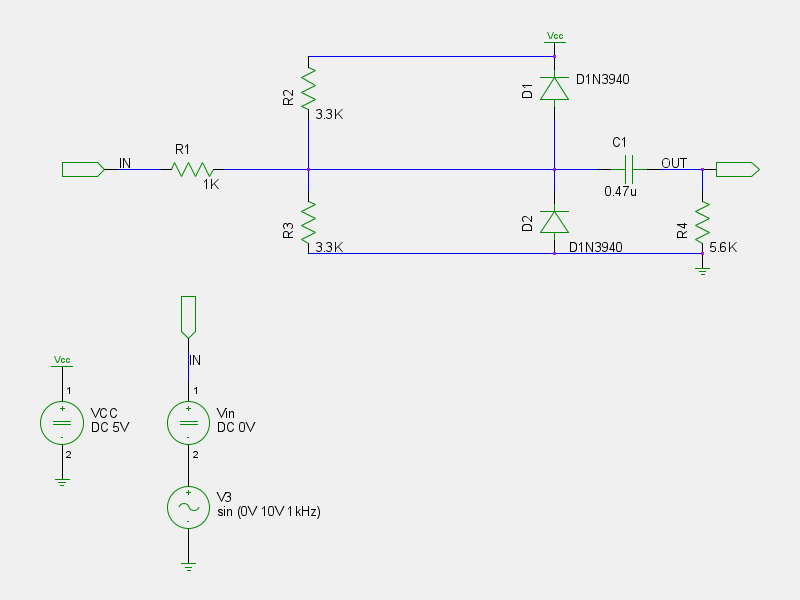
\includegraphics[width=4.5in]{diodeclipper}
}
\caption{Schematic of diode clipper circuit with DC and transient voltage sources.\label{Clipper_Schematic}}
\end{centering}
\end{figure}

Using a plain text editor (e.g., vi, Emacs, Notepad), but not a word processor (e.g., OpenOffice or Microsoft Word), 
create a file containing the netlist of figure ~\ref{Clipper_Netlist_1}. 
For this example, the file is named \texttt{clipper.cir}

The netlist in figure~\ref{Clipper_Netlist_1} illustrates some of the 
syntax of a netlist input file.  Netlists always begin with a 
title line\index{netlist!title} (\emph{e.g.\/} ``\texttt{Diode Clipper Circuit}''), and may 
contain comments\index{netlist!comments} (lines beginning with 
the ``\texttt{*}'' character), devices, and model definitions. Netlists must always end with the ``\texttt{.END}'' statement\index{netlist!\texttt{.END} statement}.

The diode clipper circuit contains two-terminal devices
(diodes, resistors, and capacitors), each of which specifies two
connecting nodes and either a model (for the diode) or a value
(resistance or capacitance).  The netlist of figure~\ref{Clipper_Netlist_1} describes the circuit shown in the schematic of figure~\ref{Clipper_Schematic}

This netlist file is not yet complete and will not run properly using \Xyce{}
(see section~\ref{Running_Xyce} for instructions on running \Xyce{}) as 
it lacks an analysis statement.  This chapter later decribes how to add the appropriate analysis statement and run the diode clipper circuit.

\begin{NetlistFigure}{Diode clipper circuit netlist}{Clipper_Netlist_1}
Diode Clipper Circuit
*
* Voltage Sources
VCC 1 0 5V
VIN 3 0 0V
* Diodes
D1 2 1 D1N3940
D2 0 2 D1N3940
* Resistors
R1 2 3 1K
R2 1 2 3.3K
R3 2 0 3.3K
R4 4 0 5.6K
* Capacitor
C1 2 4 0.47u
*
* GENERIC FUNCTIONAL EQUIVALENT = 1N3940
* TYPE:  DIODE
* SUBTYPE:  RECTIFIER
.MODEL D1N3940 D(
+         IS = 4E-10
+         RS = .105
+          N = 1.48
+         TT = 8E-7
+        CJO = 1.95E-11
+         VJ = .4
+          M = .38
+         EG = 1.36
+        XTI = -8
+         KF = 0
+         AF = 1
+         FC = .9
+         BV = 600
+        IBV = 1E-4)
*
.END
\end{NetlistFigure}

\section{DC Sweep Analysis}
\label{DC_Sweep}
This section includes an example of DC sweep
\index{analysis!DC sweep}\index{DC sweep} analysis using \Xyce{}.  
The DC response of the clipper circuit is obtained by sweeping the DC voltage 
source (\texttt{Vin}) from -10 to 15 volts in one-volt steps.
Chapter~\ref{DC_Analysis} provides more details about DC analysis,  
as does the \Xyce{} Reference 
Guide\ReferenceGuide{}.

\subsubsection{Example: DC sweep analysis}
\index{Example!DC sweep}
To set up and run a DC sweep analysis using the diode clipper circuit:
\begin{enumerate}
\item Open the diode clipper circuit netlist file (\texttt{clipper.cir}) 
using a standard text editor (\emph{e.g.\/} vi, Emacs, Notepad, \emph{etc.\/}).
\index{\texttt{.DC}}
\index{\texttt{.PRINT}!\texttt{DC}}
\item Enter the analysis control statement (as shown in the netlist in figure~\ref{Clipper_Netlist_2}):
\begin{vquote}
.DC VIN -10 15 1
\end{vquote}
\item Enter the output control statement:
\begin{vquote}
.PRINT DC V(3) V(2) V(4)
\end{vquote}
\item Save the netlist file and run \Xyce{} on the circuit. For example, to run
  serial \Xyce{}:
\begin{vquote}
 Xyce clipper.cir
\end{vquote}
\item Open the results file (\texttt{clipper.cir.prn}) and examine (or plot) the 
  output voltages that were calculated for nodes 3 (Vin), 2 and 4 (Out).
  Figure~\ref{Clipper_DCSweep} shows the output plotted as a function of the
  swept variable Vin.
\end{enumerate}

\begin{figure}[H]
\begin{centering}
\shadowbox{
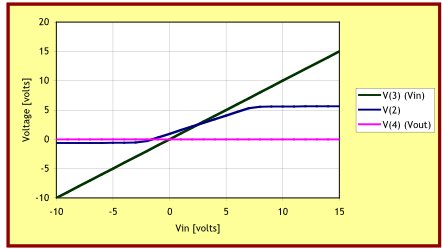
\includegraphics[width=4.5in]{clipper-dcsweep}
}
\caption{DC sweep voltages at Vin, node 2, and Vout\label{Clipper_DCSweep}}
\end{centering}
\end{figure}

\begin{NetlistFigure}{Diode clipper circuit netlist for DC sweep analysis}{Clipper_Netlist_2}
Diode Clipper Circuit with DC sweep analysis statement
*
* Voltage Sources
VCC 1 0 5V
VIN 3 0 0V
* Analysis Command
\color{XyceRed}.DC VIN -10 15 1\color{black}
* Output
\color{XyceRed}.PRINT DC V(3) V(2) V(4)\color{black}
* Diodes
D1 2 1 D1N3940
D2 0 2 D1N3940
* Resistors
R1 2 3 1K
R2 1 2 3.3K
R3 2 0 3.3K
R4 4 0 5.6K
* Capacitor
C1 2 4 0.47u
*
* GENERIC FUNCTIONAL EQUIVALENT = 1N3940
* TYPE:  DIODE
* SUBTYPE:  RECTIFIER
.MODEL D1N3940 D(
+         IS = 4E-10
+         RS = .105
+          N = 1.48
+         TT = 8E-7
+        CJO = 1.95E-11
+         VJ = .4
+          M = .38
+         EG = 1.36
+        XTI = -8
+         KF = 0
+         AF = 1
+         FC = .9
+         BV = 600
+        IBV = 1E-4)
*
.END
\end{NetlistFigure}

\section{Transient Analysis}
\label{Transient_Analysis_Sec}

This section contains an example of transient analysis\index{analysis!transient}
\index{transient analysis} in \Xyce{}.  In this example, the
DC analysis of the diode clipper circuit of the previous section has
been modified so that the input voltage source (\texttt{Vin}) is a
time-dependent sinusoidal input source.  The frequency of \texttt{Vin} is
1 kHz, and has an amplitude of 10 volts.  For more details about transient
analysis see chapter~\ref{Transient_Analysis}, or the \Xyce{} Reference 
Guide\ReferenceGuide{}.

\subsubsection{Example: transient analysis}
\index{Example!transient analysis}

To set up and run a transient analysis using the diode clipper circuit:
\begin{enumerate}
\item Open the diode clipper circuit netlist file file (\texttt{clipper.cir}) 
using a standard text editor (\emph{e.g.\/} VI, Emacs, Notepad, \emph{etc.\/}).
\item Remove DC analysis and output statements if added in the previous example (figure~\ref{Clipper_Netlist_2}).  \index{\texttt{.TRAN}}\index{\texttt{.PRINT}!\texttt{TRAN}}
\item Enter the analysis control (as shown in the netlist in figure~\ref{Clipper_Netlist_3}):
\begin{vquote}
.TRAN 2ns 2ms
\end{vquote}
\item Enter the output control statement:
\begin{vquote}
.PRINT TRAN V(3) V(2) V(4)
\end{vquote}
\item Modify the input voltage source (\texttt{Vin}) to generate the 
sinusoidal input signal:
\begin{vquote}
VIN 3 0 SIN(0V 10V 1kHz)
\end{vquote}
\item 
At this point, the netlist should look similar to the netlist in figure~\ref{Clipper_Netlist_3}.  Save the netlist file and run \Xyce{} on the circuit.  For example, to run serial \Xyce{}:
\begin{vquote}
 Xyce clipper.cir
\end{vquote}
\item Open the results file and examine (or plot) the output voltages for 
nodes 3 (\texttt{Vin}), 2, and 4 (\texttt{Out}).  The plot in
  figure~\ref{Clipper_Trans} shows the output plotted as a function of time.
\end{enumerate}
Figure~\ref{Clipper_Netlist_3} shows the modified netlist and figure~\ref{Clipper_Trans} shows the
corresponding results.

\begin{NetlistFigure}{Diode clipper circuit netlist for transient analysis}{Clipper_Netlist_3}
Diode clipper circuit with transient analysis statement
*
* Voltage Sources
VCC 1 0 5V
\color{XyceRed}VIN 3 0 SIN(0V 10V 1kHz)\color{black}
* Analysis Command
\color{XyceRed}.TRAN 2ns 2ms\color{black}
* Output
\color{XyceRed}.PRINT TRAN V(3) V(2) V(4)\color{black}
* Diodes
D1 2 1 D1N3940
D2 0 2 D1N3940
* Resistors
R1 2 3 1K
R2 1 2 3.3K
R3 2 0 3.3K
R4 4 0 5.6K
* Capacitor
C1 2 4 0.47u
*
* GENERIC FUNCTIONAL EQUIVALENT = 1N3940
* TYPE:  DIODE
* SUBTYPE:  RECTIFIER
.MODEL D1N3940 D(
+         IS = 4E-10
+         RS = .105
+          N = 1.48
+         TT = 8E-7
+        CJO = 1.95E-11
+         VJ = .4
+          M = .38
+         EG = 1.36
+        XTI = -8
+         KF = 0
+         AF = 1
+         FC = .9
+         BV = 600
+        IBV = 1E-4)
*
.END

\end{NetlistFigure}

\begin{figure}[H]
  \begin{centering}
    \shadowbox{
      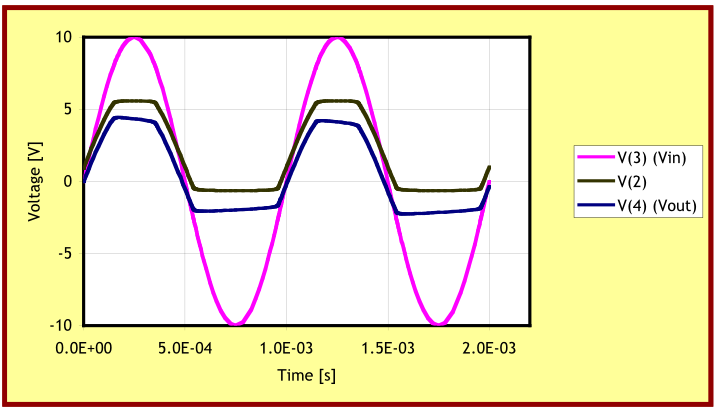
\includegraphics[width=4.5in]{clipper-trans}
    }
    \caption{Sinusoidal input signal and clipped outputs\label{Clipper_Trans}}
  \end{centering}
\end{figure}

%%% Local Variables:
%%% mode: latex
%%% End:
% END of Xyce_UG_ch03.tex ************

\cleardoublepage
% Sandia National Laboratories is a multimission laboratory managed and
% operated by National Technology & Engineering Solutions of Sandia, LLC, a
% wholly owned subsidiary of Honeywell International Inc., for the U.S.
% Department of Energy’s National Nuclear Security Administration under
% contract DE-NA0003525.

% Copyright 2002-2019 National Technology & Engineering Solutions of Sandia,
% LLC (NTESS).

%%-------------------------------------------------------------------------
%% Purpose        : Main LaTeX Xyce Users' Guide
%% Special Notes  : Graphic files (pdf format) work with pdflatex.  To use
%%                  LaTeX, we need to use postscript versions.  Not sure why.
%% Creator        : Scott A. Hutchinson, Computational Sciences, SNL
%% Creation Date  : {05/23/2002}
%%
%%-------------------------------------------------------------------------

\chapter{Netlist Basics}
\label{Netlist_Basics}

\chapteroverview{Chapter Overview}
{
This chapter contains introductory material on netlist syntax and usage.
Sections include:
\begin{XyceItemize}
\item Section~\ref{General_Overview} \emph{General Overview}
\item Section~\ref{Available_Devices} \emph{Devices Available for Simulation}
\item Section~\ref{Parameters_Expressions} \emph{Parameters and Expressions}
\end{XyceItemize}
}

\section{General Overview}
\label{General_Overview}

\subsection{Introduction}

Using a netlist\index{netlist} to describe a circuit for \Xyce{} is the primary method for running a circuit
simulation\index{circuit!simulation}.  Netlist support within \Xyce{}
largely conforms to that used by Berkeley SPICE 3F5\index{SPICE} with
several new options for controlling functionality unique to \Xyce{}.

In a netlist, the circuit is described by a set of \emph{element
lines\/} defining circuit elements\index{circuit!elements} and their associated parameters, the circuit topology\index{circuit!topology} (i.e., the connection of the circuit elements), and a variety of control options for the simulation. 
The first line in the netlist
file must be a title\index{netlist!title line} and the last line must
be ``\texttt{.END}''\index{netlist!\texttt{.END}}.  Between these two
constraints, the order of the statements is irrelevant.

\subsection{Nodes}
\index{nodes}
\index{nodes!global}
\index{global nodes}
\index{netlist!nodes}

Nodes and elements form the foundation for the circuit topology. Each node represents a point in the circuit that is connected to the leads of multiple elements (devices). Each lead of every element is connected to a node, and each node is connected to multiple element leads.

A node is simply a named point in the circuit. The naming of normal nodes is only known within the level of circuit hierarchy where they appear; normal nodes defined in the main circuit are not visible to subcircuits, nor are nodes defined in a subcircuit visible to the top-level circuit. Nodes can be passed into subcircuits through an argument list, and in this case subcircuits are given limited access to nodes from the upper-level circuit.  

\subsubsection{Global Nodes}
For cases where a particular node is used widely throughout various
subcircuits it can be more convenient to use a global node, which is
referenced by the same name throughout the circuit.  This is often the
case for power rails such as \texttt{VDD} or \texttt{VSS}.

Global nodes start with the prefix \texttt{\$G}.  Examples of global node names would be:
{\texttt \$G\_VDD} or \texttt{\$G1}.  Nodes or global nodes require no declaration, as they are declared implicitly by appearing in \emph{element lines\/}.

For compatibility with HSPICE, the \texttt{.GLOBAL} command can be 
used to define global nodes that do not start with the prefix ``\$G''.
Consult the \Xyce{} Reference Guide\ReferenceGuide{} for more details. 

\subsection{Elements}
\index{elements}
\index{netlist!elements}

An \emph{element line\/} defines each circuit element instance. While each element type determines the specific format, the general format is given by:
\begin{vquote}
<type><name> <node information> <element information...>
\end{vquote}
The \texttt{<type>} must be a letter (A through Z) with the
\texttt{<name>} immediately following.  For example, \texttt{RARESISTOR}
specifies a device of type ``R'' (for ``Resistor'') with a name
\texttt{ARESISTOR}.  Nodes are separated by spaces, and additional
element information required by the device is given after the node
list as described in the Netlist Reference section of the \Xyce{}
Reference Guide\ReferenceGuide{}.
\Xyce{} ignores character case when reading 
a netlist such that \texttt{RARESISTOR} is equivalent to \texttt{raresistor}.  The 
only exception to this case insensitivity occurs when including external files in a netlist  where 
the filename specified in the netlist must have the same case as the actual filename.

A number field may be an integer or a floating-point value.  Either one may be
followed by one of the following \index{netlist!scaling factors} scaling
factors shown in Table~\ref{scalefactors}:

\begin{table}[H]
  \caption{Scaling factors.}\label{scalefactors}
  \center{
    \begin{tabularx}{3in}{|W|W|} \hline
      \rowcolor{XyceDarkBlue} \color{white} \bf Symbol & \color{white}\bf
      Equivalent Value \\ \hline
      \verb+T+ & $10^{12}$ \\ \hline
      \verb+G+ & $10^9$ \\ \hline
      \verb+Meg+ & $10^6$ \\ \hline
      \verb+X+ & $10^6$ \\ \hline
      \verb+K+ & $10^3$ \\ \hline
      \verb+mil+ & $25.4^{-6}$ \\ \hline
      \verb+m+ & $10^{-3}$ \\ \hline
      \verb+u+ ($\mu$) & $10^{-6}$ \\ \hline
      \verb+n+ & $10^{-9}$ \\ \hline
      \verb+p+ & $10^{-12}$ \\ \hline
      \verb+f+ & $10^{-15}$ \\ \hline
    \end{tabularx}
  }
\end{table}

Node information is given in terms of \index{netlist!node names} \index{node
  names} node names, which are character strings.  One key
requirement is that the \index{ground nodes} ground node is named `\texttt{0}'.
(Note: Consult the \Xyce{} Reference Guide\ReferenceGuide{} for more details on 
allowed characters in both node names and device names.)
There is one restriction on the \index{circuit!topology} \index{topology}
circuit topology: there can be no loop of voltage sources and/or inductors.
In addition to this requirement, the following additional topology 
constraints are highly recommended:
\begin{XyceItemize}
\item Every node has a DC path to ground.
\item Every node has at least two connections (with the exception of
  unterminated transmission lines and MOSFET substrate nodes).
\end{XyceItemize}
While \Xyce{} can theoretically handle netlists that violate the above two 
constraints, such topologies are typically the result of human error in 
creating a netlist file, and will often lead to convergence failures.  Chapter~\ref{Preprocess_Chap} provides more information on this topic.


The following line provides an example of an element line that defines a
resistor between nodes \texttt{1} and \texttt{3} with a resistance value 
of $10 \mbox{k}\Omega$.

\Example{\texttt{RARESISTOR 1 3 10K}}

\subsubsection{Title, Comments and End}
\index{netlist!first line special} 

The first line of the netlist is the title line\index{netlist!title
line} of the netlist.  This line is treated as a comment even if it
does not begin with an asterisk.  It is a common mistake to forget the
meaning of this first line and begin the circuit elements on the first
line; doing so will probably result in a parsing error.

\Example{\texttt{Test RLC Circuit}}

The ``\verb+.END+''\index{netlist!end line} line must be the last line in the
netlist.

\Example{\texttt{.END}}
\index{comments in a netlist}
Comments\index{netlist!comments} are supported in netlists and are indicated by
placing an asterisk at the beginning of the comment line.  They may occur
anywhere in the netlist \emph{but} they must be at the beginning of a line.
\Xyce{} also supports \emph{in-line\/} comments\index{netlist!in-line comments}.  An in-line comment is designated by a semicolon and may occur on any line. \Xyce{} ignores everything after a semicolon. \Xyce{} considers lines beginning with leading whitespace as comments
unless the first character after the whitespace is a \verb|+| symbol, in which case it treats the line as a continuation. 

\Example{\texttt{* This is a netlist comment.}}

\Example{\bf{WRONG:}\texttt{.DC .... * This type of in-line comment is \emph{not
      supported}.}}

\Example{\texttt{.DC .... ; This type of in-line comment is supported.}}

\subsubsection{Continuation Lines}
Continuation lines begin with a \verb|+| symbol, and their contents are appended to those of the previous line.  If the previous line or lines were comments, the continuation line is
appended to the first noncomment line preceding it.  Continuation lines can have leading whitespace before the \verb|+| symbol.

\subsubsection{Netlist Commands}
Command elements\index{netlist!command elements} are used to describe the
analysis being defined by the netlist.  Examples include analysis types,
initial conditions, device models, and output control.
The \Xyce{} Reference Guide\ReferenceGuide{} contains a reference for these commands.

\Example{\texttt{.PRINT TRAN V(Vout)}}

\subsubsection{Analog Devices}
\Xyce{}-supported analog\index{netlist!analog devices}\index{device!analog} devices
include most of the standard circuit components normally found in circuit
simulators, such as SPICE 3F5, PSpice, etc., plus several Sandia-specific
devices.

\Example{\texttt{D\_CR303 N\_0065 0 D159700}}

The \Xyce{} Reference Guide\ReferenceGuide{} provides more information concerning its supported devices.

\section{Devices Available for Simulation}
\label{Available_Devices}

The analog devices available in \Xyce{} include all of the standard circuit
components needed for most analog circuits.  User-defined models may be
implemented using the \index{netlist!model definition}\index{\texttt{.MODEL}}
\texttt{.MODEL} (model definition) statement, and macromodels can be created as
subcircuits using the \index{netlist!subcircuit}
\texttt{.SUBCKT}\index{\texttt{.SUBCKT}} (subcircuit) statement.

In addition to the traditional analog devices, which are modeled in \Xyce{} by
sets of coupled differential algebraic equations, \Xyce{} also supports digital
\index{device!digital} \index{behavioral model} \index{device!behavioral model}
behavioral models. The digital devices are behavioral devices in the sense that
they rely on truth tables to determine their outputs. Once one or more of a
digital device's inputs go past user-specified thresholds, its outputs will
change according to its truth table after a user-specified delay time. The
impedance characteristics of the inputs and outputs of the digital devices are
modeled with RC time constants. 

\Xyce{} also include TCAD devices, which solve a coupled set of partial
differential equations (PDEs), discretized on a mesh. The use of these devices
are described in detail in Chapter~\ref{PDE_Devices}.

The device element statements in the netlist always start with the name of the
individual \index{device!instance} device instance. The first letter of the
name determines the device type. The format of the subsequent information
depends on the device type and its parameters.  Table~\ref{Device_Summary}
provides a quick reference to the analog devices and their netlist formats as
supported by \Xyce{}. Except where noted, the devices are based upon those
found in ~\cite{Grove:1967}. The \Xyce{} Reference Guide\ReferenceGuide{}
provides a complete description of the syntax for all the supported devices.

\LTXtable{\textwidth}{analogtbl}


\section{Parameters and Expressions}
\label{Parameters_Expressions}

In addition to explicit values, the user may use parameters and expressions to symbolize numeric values in the circuit design.

\subsection{Parameters}
\index{netlist!parameters}

A parameter is a symbolic name representing a numeric value. Parameters must start with a letter or underscore. The characters after the first can be letter, underscore, or digits. Once a parameter is defined (by having its name declared and having a value assigned to it) at a particular level in the circuit hierarchy, it can be used to represent circuit values at that level or any level directly beneath it in the circuit hierarchy. One way to use parameters is to apply the same value to multiple part instances.


\subsection{How to Declare and Use Parameters}
\index{netlist!parameters}

For using a parameter in a circuit, one must:
\begin{XyceItemize}
\item Define the parameter using a \verb+.PARAM+ statement within a netlist
\item Replace an explicit value with the parameter in the circuit
\end{XyceItemize}
 \Xyce{} reserves the following keywords that may not be used as parameter names:
\begin{XyceItemize}
\item \verb+Time+
\item \verb+Freq+ 
\item \verb+Vt+
\item \verb+Temp+
\item \verb+GMIN+
\end{XyceItemize}

\texttt{Time}, \texttt{TEMP}, \texttt{Vt} and \texttt{GMIN} are
reserved and defined as ``special variables'', and may be used in
B source expressions.  The use of the \texttt{FREQ} special variable
in B source expressions is not supported.

\subsubsection{Example:  Declaring a parameter}
\index{Example!declaring parameters}
\index{parameter!declaring}
\begin{enumerate}
\item Locate the level in the circuit hierarchy at which the \verb+.PARAM+
  statement declaring a parameter will be placed. To declare a parameter capable of being used anywhere in the netlist, place the \verb+.PARAM+ statement at the top-most level of the circuit.
\item Name the parameter and give it a value. The value can be numeric or given
  by an expression:
  \begin{vquote}
.SUBCKT subckt1 n1 n2 n3
.PARAM res = 100
*
* other netlist statements here
*
.ENDS
\end{vquote}
\item NOTE: The parameter \emph{res} can be used anywhere within the subcircuit
  \texttt{subckt1}, including subcircuits defined within it, but cannot be used outside
  of \texttt{subckt1}.
\end{enumerate}

\subsubsection{Example:  Using a parameter in the circuit}
\index{Example!using parameters}
\index{parameter!using in expressions}
\begin{enumerate}
\item Locate the numeric value (a device instance parameter value, model parameter value, etc.) that is to be replaced by a parameter.  
\item Replace the numeric value with the parameter name contained within braces
  (\{\}) as in:
\begin{vquote}
R1 1 2 \{res\}
\end{vquote}
\end{enumerate}

NOTE:	Ensure the value being replaced remains accessible within the current hierarchy level.

\subsubsection{Limitations on parameter definitions}

As chapter~\ref{Behavioral_Modeling} describes, there is considerable flexibility in the use of parameters. They can be set to expressions containing other parameters, and can be passed down the hierarchy into subcircuits. Fundamentally, however, parameters are constants evaluated at the beginning of a run; therefore, all terms in the expression defining the parameter must be constants known at the beginning of the run. It is not legal to use time-dependent or frequency-dependent expressions in parameter declarations (either by including voltage nodes or currents, or by including references to the special variables \texttt{TIME} or \texttt{FREQ}).

Parameters defined within a given scope can be used in any expression within that scope. The only limitation on ordering is for the use of a parameter in an expression that defines the value of another parameter. In that case, all parameters used in the expression must be defined before being used to define another parameter. So, in the following example:

  \begin{vquote}
R1  1  0  \{B+C\} ; OK because the expression is not used to define a param
.PARAM A=3
.PARAM B=\{A+1\}  ; OK because A is defined above
.PARAM D=\{C+2\}  ; Illegal because C is not yet known
.PARAM C=2
\end{vquote}

\subsection{Global Parameters}
\index{netlist!global parameterss}
\index{global parameters}
\index{parameter!global}
 
A normal parameter defined at the main circuit level will have global scope.
Such parameters suffer from limitations, such as: (1) they are constant during the simulation,
and (2) the parameter may redefined within a subcircuit, which would change the value
in the subcircuit and below.  Global parameters address these limitations.

A global parameter differs from a normal parameter in that it can only be defined
at the main circuit level, and it is allowed to change during a simulation.  Global parameters
act as variables rather than constants during the simulation.  Examples of some
global parameter usages are:
  \begin{vquote}
.param dTdt=100
.global_param T=\{27+dTdt*time\}
R1  1  2  RMOD TEMP=\{T\}

or

.global_param T=27
R1  1  2  RMOD TEMP=\{T\}
C1  1  2  CMOD TEMP=\{T\}
.step T 20 50 10
\end{vquote}

In these examples, T is used to represent an environmental variable that changes.

NOTE:	Normal parameters may be used in expressions defining global parameters, but the opposite is not allowed.

\subsection{Expressions}
\index{netlist!expressions}
\index{expressions}

In \Xyce{}, an expression is a mathematical relationship that may be
used any place one would use a number (numeric or boolean).  Except in
the case of expressions used in analog behavioral modeling sources
(see chapter~\ref{Behavioral_Modeling}) \Xyce{} evaluates the
expression to a value when it reads in the circuit netlist, not each
time its value is needed. Therefore, all terms in an expression must be known at the beginning of a run.

To use an expression in a circuit netlist:
\index{netlist!using expressions}
\index{expressions!using}
\begin{enumerate}
\item Locate the value to be replaced (component, model parameter, etc.).
\item Substitute the value with an expression using the \texttt{\{\}}
  syntax:
\begin{quote}
  \texttt{\{{\it expression\/}\}}%
\end{quote}
where \texttt{\it expression\/} can contain any of the
following:\index{expressions!valid constructs}
\begin{XyceItemize}
\item Arithmetic and logical operators.
\item Arithmetic, trigonometric, or SPICE-type functions.
\item User-defined functions.
\item User-defined parameters within scope.
\item Literal operands.
\end{XyceItemize}
The braces (\texttt{\{\}}) instruct \Xyce{} to evaluate the expression and use
the resulting value. Additional time-dependent constructs are available in expressions used in analog behavioral modeling sources (see chapter~\ref{Behavioral_Modeling}).    Complete documentation of supported functions and operators may be found in the \Xyce{} Reference Guide\ReferenceGuide{}.

\index{analog behavioral modeling (ABM)}
\index{behavioral model} 
\index{behavioral model!analog behavioral modeling (ABM)}

\end{enumerate}

\subsubsection{Example:  Using an expression}
\index{Example!using expressions}
\index{expressions!example}
Scaling the DC voltage of a $12V$ independent voltage source, designated
\verb+VF+, by some factor can be accomplished by the following netlist
statements (in this example the factor is $1.5$):
\begin{vquote}
.PARAM FACTORV=1.5
VF 3 4 \{FACTORV*12\}
\end{vquote}
\Xyce{} will evaluate the expression to $12 * 1.5$ or $18\:\mbox{volts}$.


%%% Local Variables:
%%% mode: latex
%%% End: 

% END of Xyce_UG_ch04.tex ************

\cleardoublepage
% Sandia National Laboratories is a multimission laboratory managed and
% operated by National Technology & Engineering Solutions of Sandia, LLC, a
% wholly owned subsidiary of Honeywell International Inc., for the U.S.
% Department of Energy’s National Nuclear Security Administration under
% contract DE-NA0003525.

% Copyright 2002-2020 National Technology & Engineering Solutions of Sandia,
% LLC (NTESS).

%%-------------------------------------------------------------------------
%% Purpose        : Main LaTeX Xyce Users' Guide
%% Special Notes  : Graphic files (pdf format) work with pdflatex.  To use
%%                  LaTeX, we need to use postcript versions.  Not sure why.
%% Creator        : Scott A. Hutchinson, Computational Sciences, SNL
%% Creation Date  : {05/23/2002}
%%
%%-------------------------------------------------------------------------

\chapter{Working with Subcircuits and Models}
\label{Models}

\chapteroverview{Chapter Overview}
{
This chapter provides model examples and summarizes ways to create and
modify models.  Sections include:
\begin{XyceItemize}
\item Section~\ref{Model_Def}, {\em Model Definition}
\item Section~\ref{Subcircuit_Sect}, {\em Subcircuit Creation}
\item Section~\ref{Model_Organization}, {\em Model Organization}
\item Section~\ref{Model_Interpolation}, {\em Model Interpolation}
\end{XyceItemize}
}

\section{Model Definitions}
\label{Model_Def}
\index{model!definition}

A model describes the electrical performance of a {\em part}, such as
a specific vendor's version of a 2N2222 transistor.  To simulate a
part requires specification of {\em simulation properties}.  
These properties define the model of the part.

Depending on the given device type and the requirements of the circuit
design, a model is specified using a model parameter set, a subcircuit
netlist, or both.

In general, {\em model parameter sets} define the parameters used in ideal
models of specific device types, while {\em subcircuit netlists} allow the user
to combine ideal device models to simulate more complex effects.  For example,
one could simulate a bipolar transistor using the \Xyce{} BJT device by specifying
model parameters extracted to fit the simulation behavior to the behavior of
the part used. One could also develop a subcircuit macro-model of a capacitor
that adds effects such as lead inductance and resistance to the basic capacitor
device.

Both methods of defining a model use a netlist format, with precise
syntax rules.  In this section we give an overview of how to define
model parameter sets in \Xyce{}.  A subsequent subsection will provide a
similar overview of how to define subcircuit models.  For full
details, consult the \Xyce{} Reference Guide\ReferenceGuide.

\paragraph{Defining models using model parameters}

Although \Xyce{} has no built-in part models,  models can be defined for a
device by changing some or all of the {\em model parameters} from their
defaults via the \texttt{.MODEL} statement. For example:

\begin{vquote}
 \texttt{M5 3 2 1 0 MLOAD1}
 \texttt{.MODEL MLOAD1 NMOS (LEVEL=3 VTO=0.5 CJ=0.025pF)}
\end{vquote}

This example defines a MOSFET device \texttt{M5} that is an instance of a part
described by the model parameter set \texttt{MLOAD1}.  The \texttt{MLOAD1}
parameter set is defined in the \texttt{.MODEL} statement.

Most device types in \Xyce{} support some form of model parameters.  Consult
the \Xyce{} Reference Guide\ReferenceGuide{} for the model parameters supported
by each device type.

\paragraph{Defining models using subcircuit netlists}

In \Xyce{}, models may also be defined using the
\texttt{.SUBCKT}/\texttt{.ENDS} subcircuit syntax. This syntax allows the
creation of {\em Netlists}, which define the configuration and function of the
part, and the use of {\em Variable input parameters}, which can be used to
create device-specific implementations of the model.  The \texttt{.SUBCKT}
syntax, and an example of how to use \texttt{.SUBCKT} to implement a model, is
given in Section~\ref{Subcircuit_Sect}.

\clearpage
\section{Subcircuit Creation}
\label{Subcircuit_Sect}
\index{\texttt{.SUBCKT}}
\index{subcircuits}

A subcircuit can be created within \Xyce{} using the \texttt{.SUBCKT} keyword.
The \texttt{.ENDS} keyword is used to mark the end of the subcircut. All the
lines between the two keywords are considered to be part of the subcurcuit.  
Figure~\ref{Subcircuit_Example} provides an example of how a subcircuit is
defined and used.

\begin{figure}[H]
\begin{centering}
\shadowbox{
\begin{minipage}{0.8\textwidth}
\begin{vquote}
****other devices
X5 5  6  7  8 l3dsc1 PARAMS: ScaleFac=2.0
X6 9 10 11 12 l3dsc1
****more netlist commands

*** SUBCIRCUIT: l3dsc1
*** Parasitic Model: microstrip
*** Only one segment
.SUBCKT l3dsc1 1 3 2 4 PARAMS: ScaleFac=1.0
C01 1 0 4.540e-12
RG01 1 0 7.816e+03
L1 1 5 3.718e-08
R1 5 2 4.300e-01
C1 2 0 4.540e-12
RG1 2 0 7.816e+03
C02 3 0 4.540e-12
RG02 3 0 7.816e+03
L2 3 6 3.668e-08
R2 6 4 4.184e-01
C2 4 0 4.540e-12
RG2 4 0 7.816e+03
CM012 1 3 5.288e-13
KM12 L1 L2 2.229e-01
CM12 2 4 \{5.288e-13*ScaleFac\}
.ENDS
\end{vquote}
\end{minipage}
}
\caption{Example subcircuit model.\label{Subcircuit_Example}}
\index{Example!subcircuit definition}
\end{centering}
\end{figure}

In this example, a subcircuit model named \texttt{l3dsc1}, which implements one
part of a microstrip transmission line, is defined between the
\texttt{.SUBCKT}/\texttt{.ENDS} lines; and two different instances of the
subcircuit are used in the \texttt{X} lines.  This somewhat artificial example
shows how input parameters are used, where the last capacitor in the subcircuit
is scaled by the input parameter \texttt{ScaleFac}.  If input parameters are
not specified on the \texttt{X} line (as in the case of device \texttt{X6}),
then the default values specified on the \texttt{.SUBCKT} line are used.
Non-default values are specified on the \texttt{X} line using the
\texttt{PARAMS:} keyword.  Consult the \Xyce{} Reference Guide\ReferenceGuide{}
for precise syntax.

In addition to devices, a subcircuit may contain definitions, such as models
via the \texttt{.MODEL} statement, parameters via the \texttt{.PARAM}
statement, and functions via the \texttt{.FUNC} statement.  \Xyce{} also
supports the definition of one or more subcircuits within another subcircuit.
\index{subcircuits!hierarchy} Subcircuits can be nested to an arbitrary extent,
where one subcircuit can contain another subcircuit, which can contain yet
another subcircuit, and so on.

The creation of nested subcircuits requires an understanding of ``scope,''
\index{subcircuits!scope} such that each subcircuit defines the scope for the
definitions it contains.  That is, {\em the definitions contained within a
subcircuit can be used within that subcircuit and within any subcircuit it
contains, but not at any higher level.}  Definitions occurring in the main
circuit have global scope and can be used anywhere in the circuit.  A name,
such as a model, parameter, function, or subcircuit name, occurring in a
definition at one level of a circuit hierarchy can be redefined at any lower
level contained directly by that subcircuit.  In this case, the new definition
applies at the given level and those below.

\subsection{Examples of Scoping for Parameters, Models and Functions}
\index{parameter!scope}\index{model!scope}\index{subcircuit!scope}
The idea of ``scope'' may be best illustrated by examples.  This section gives
example for parameters and models.  However, this discussion also applies to
functions (defined with \texttt{.FUNC} statements). 

In the netlist provided
in Figure~\ref{Subcircuit_Example_2}, the model named \texttt{MOD1} can be used
in subcircuits \texttt{SUB1} and \texttt{SUB2}, but not in the subcircuit
\texttt{SUB3}. The parameter \texttt{P1} has a value of $10$ in subcircuit
\texttt{SUB1} and a value of $20$ in subcircuit \texttt{SUB2}. In subcircuit
\texttt{SUB3}, \texttt{P1} has no meaning.  In addition, \texttt{MOD1}
and \texttt{P1} would have no meaning at the main circuit level.

\begin{figure}[H]
\begin{centering}
\shadowbox{
\begin{minipage}{0.8\textwidth}
\begin{vquote}
.SUBCKT SUB1 1 2 3 4
.MODEL MOD1 NMOS(LEVEL=2)
.PARAM P1=10
*
* subcircuit devices omitted for brevity
*
.SUBCKT SUB2 1 3 2 4
.PARAM P1=20
*
* subcircuit devices omitted for brevity
*
.ENDS
.ENDS

.SUBCKT SUB3 1 2 3 4
*
* subcircuit devices omitted for brevity
*
.ENDS
\end{vquote}
\end{minipage}
}
\caption{Example subcircuit hierarchy, with scoping.\label{Subcircuit_Example_2}}
\index{Example!subcircuit model hierarchy with model and parameter scoping}
\end{centering}
\end{figure}

In the netlist provided in Figure~\ref{Subcircuit_Example_3}, the parameters
\texttt{P2} and \texttt{P3} are defined in the main circuit.  So, \texttt{P2}
is accessible in subcircuit \texttt{SUB4}, and has a value of 5 there. The
parameter \texttt{P3} was redefined in the context of subcircuit \texttt{SUB4}.
So, \texttt{P3} has a value of 10 in the main circuit, and a value of 15
in the context of subcircuit \texttt{SUB4} and any subcircuit subsequently 
defined within subcircuit \texttt{SUB4}.  
\begin{figure}[H]
\begin{centering}
\shadowbox{
\begin{minipage}{0.8\textwidth}
\begin{vquote}
* parameters defined in main circuit
.PARAM P2=5
.PARAM P3=10

.SUBCKT SUB4 1 2 3 4
.PARAM P3=15
*
* subcircuit devices omitted for brevity
*
.ENDS
\end{vquote}
\end{minipage}
}
\caption{Example subcircuit, with parameter definition override.\label{Subcircuit_Example_3}}
\index{Example!subcircuit, with parameter definition override}
\end{centering}
\end{figure}

In the netlist provided in Figure~\ref{Subcircuit_Example_4}, the 
definition of subcircuit \texttt{SUB5} defines the argument \texttt{A1}.
The subcircuit instance \texttt{X1} would use the default value of 5
for \texttt{A1}.  So the resistance value of device \texttt{X1:R1}
would be 5.  The subcircuit instance \texttt{X2} uses the specified
\texttt{A1} value of 10. So the resistance value of device \texttt{X2:R1}
would be 10.  Another key point about ``scope'' is that node, device, and
model names are scoped to the subcircuit in which they are defined. 
So, It is allowable to use names in a subcircuit that has been previously
used in either the main circuit netlist or in other subcircuit definitions.   
When the subcircuits are flattened (expanded to become part of the main 
netlist), all of their names are given prefixes via their subcircuit 
instance names. For example, device \texttt{R1} in subcircuit \texttt{X1} 
becomes the unique device name X1:R1 after expansion. 
\begin{figure}[H]
\begin{centering}
\shadowbox{
\begin{minipage}{0.8\textwidth}
\begin{vquote}
* subcircuit instance lines
X1 a b  SUB5 
X2 e f SUB5 PARAMS: A1=10
R1 1 2 2

* Note use of \{\} around A1 and FSIN parameters in
* the body of the subcircuit definition.
.SUBCKT SUB5 1 2 PARAMS: A1=5 FSIN=1
VSIN 1 g SIN(0 1V \{FSIN\} 0)
R1 g 2 \{A1\}
.ENDS
\end{vquote}
\end{minipage}
}
\caption{Example subcircuit, with PARAMS arguments.\label{Subcircuit_Example_4}}
\index{Example!subcircuit, with PARAMS arguments}
\end{centering}
\end{figure}

\clearpage
\section{Model Organization}
\label{Model_Organization}
\index{model!model organization}

While it is always possible to make a self-contained netlist in which
all models for all parts are included along with the circuit
definition, \Xyce{} provides a simple mechanism to conveniently organize
frequently used models into separate model libraries.  Models are simply
collected into model library files, and then accessed by netlists as needed by
inserting an \texttt{.INCLUDE}\index{\texttt{.INCLUDE}} directive.  This
section describes that process in detail.

\subsection{Model Libraries}

Device model and subcircuit definitions may be organized into model
libraries as text files (similar to netlist files) with one or more model
definitions. Many users choose to name model library files ending with
\texttt{.lib}, but they may be named using any convention.

In general, most users create model libraries files that include similar model
types.  In these files, the {\em header comments} describe the models therein.  

\subsection{Model Library Configuration using \texttt{.INCLUDE}}

\Xyce{} uses model libraries by inserting an \texttt{.INCLUDE}
statement into a netlist.  Once a file is included, its contents become
available to the netlist just as if the entire contents had been
inserted directly into the netlist.

As an example, one might create the following model library file
called \texttt{bjtmodels.lib}, containing \texttt{.MODEL} statements for
common types of bipolar junction transistors:

\begin{vquote}
*bjtmodels.lib
* Bipolar transistor models
.MODEL Q2N2222 NPN (Is=14.34f Xti=3 Eg=1.11 Vaf=74.03 Bf=5 Ne=1.307
+  Ise=14.34f Ikf=.2847 Xtb=1.5 Br=6.092 Nc=2 Isc=0 Ikr=0 Rc=1
+  Cjc=7.306p Mjc=.3416 Vjc=.75 Fc=.5 Cje=22.01p Mje=.377 Vje=.75
+  Tr=46.91n Tf=411.1p Itf=.6 Vtf=1.7 Xtf=3 Rb=10)

.MODEL 2N3700 NPN (IS=17.2E-15 BF=100)

.MODEL 2N2907A PNP (IS=1.E-12 BF=100)
\end{vquote}

The models \texttt{Q2N2222}, \texttt{2N3700} and \texttt{2N2907A} could then be
used in a netlist by including the \texttt{bjtmodels.lib} file.

\begin{vquote}
.INCLUDE "bjtmodels.lib"
Q1 1 2 3 Q2N2222
Q2 5 6 7 2N3700
Q3 8 9 10 2N2907A
*other netlist entries
.END
\end{vquote}

Because the contents of an included file are simply inserted into the netlist
at the point where the \texttt{.INCLUDE} statement appears, the scoping rules
for \texttt{.INCLUDE} statements are the same as for other types of definitions
as outlined in the preceding subsections. 

NOTE:	The path to the library file is assumed to be relative to the execution
directory, but absolute pathnames are permissible.  The entire file name,
including its ``extension'' must be specified.  There is no assumed default
extension.

\subsection{Model Library Configuration using \texttt{.LIB}}

An alternative technique for organizing model libraries employs the
\texttt{.LIB} command.  With \texttt{.LIB}, a library file can contain
multiple versions of a model and specific versions may be selected at
the top level using a keyword on the \texttt{.LIB} line.  

There are two different uses for the \texttt{.LIB} command.  In the
main netlist, \texttt{.LIB} functions in a similar manner to
\texttt{.INCLUDE}: it reads in a file.  Inside that file,
\texttt{.LIB} and \texttt{.ENDL} are used to specify blocks of model
code that may be included independently of other parts of the same
file.

As an example, if you had two different 2N2222 transistor models extracted 
at different \textrmb{TNOM} values, you could define them in a model library
inside \texttt{.LIB}/\texttt{.ENDL} pairs:

\begin{vquote}
* transistors.lib file
.lib roomtemp
.MODEL Q2N2222 NPN (TNOM=27 Is=14.34f Xti=3 Eg=1.11 Vaf=74.03 Bf=5 Ne=1.307
+  Ise=14.34f Ikf=.2847 Xtb=1.5 Br=6.092 Nc=2 Isc=0 Ikr=0 Rc=1
+  Cjc=7.306p Mjc=.3416 Vjc=.75 Fc=.5 Cje=22.01p Mje=.377 Vje=.75
+  Tr=46.91n Tf=411.1p Itf=.6 Vtf=1.7 Xtf=3 Rb=10)
.endl

.lib hightemp
.MODEL Q2N2222 NPN (TNOM=55 [...parameters omitted for brevity...])
.endl
\end{vquote}

Note that both models are given identical names, but are enclosed
within \texttt{.LIB}/\texttt{.ENDL} pairs with different names.  When
this file is used in a netlist, a specific model can be used by
specifying it on the \texttt{.LIB} line in the main netlist.

\begin{vquote}
*This netlist uses only the high temperature model from the library
.lib transistors.lib hightemp
Q1 collector base emitter Q2N2222
[...]
\end{vquote}

The exact format and usage of the \texttt{.LIB} command is documented in the
\Xyce{} Reference Guide\ReferenceGuide{}.

\section{Model Interpolation}
\label{Model_Interpolation}
\index{model!model interpolation}
\index{model!tempmodel}

Traditionally, SPICE simulators handle thermal effects by coding
the temperature dependence of model parameters into each device.  These
expressions modify the nominal device parameters given in the
\texttt{.MODEL} card when the ambient temperature is not equal to
\textrmb{TNOM}, the temperature at which the nominal device parameters
were extracted.

These temperature correction equations may be reasonable at
temperatures close to \textrmb{TNOM}, but Sandia users of \Xyce{} have
found them inadequate when simulations must be performed over a wide
range of temperatures.  To address this inadequacy, \Xyce{} implements
a model interpolation option that allows the user to specify multiple
\texttt{.MODEL} cards, each extracted from real device measurements at
a different \textrmb{TNOM}.  From these model cards, \Xyce{} will
interpolate parameters based on the ambient temperature using either
piecewise linear or quadratic interpolation.

Interpolation of models is accessed through the model parameter
\textrmb{TEMPMODEL} in the models that support this capability.  In the netlist,
a base model is specified, and is followed by multiple models at other
temperatures.  

Interpolation of model cards in this fashion is implemented in the BJT
level 1, JFET, MESFET, and MOSFETS levels 1-6, 10, and 18.

The use of model interpolation is best shown by example:

\begin{vquote}
Jtest 1a 2a 3 SA2108 TEMP= 40
*
.MODEL SA2108 PJF ( TEMPMODEL=QUADRATIC TNOM = 27
+ LEVEL=2 BETA= 0.003130 VTO = -1.9966 PB = 1.046
+ LAMBDA = 0.00401 DELTA = 0.578; THETA = 0;
+ IS = 1.393E-10          RS = 1e-3)
*
.MODEL SA2108 PJF ( TEMPMODEL=QUADRATIC TNOM = -55
+ LEVEL=2 BETA = 0.00365 VTO = -1.9360 PB = 0.304
+ LAMBDA = 0.00286 DELTA = 0.2540 THETA = 0.0
+ IS = 1.393E-10 RD = 0.0 RS = 1e-3)
* 
.MODEL SA2108 PJF ( TEMPMODEL=QUADRATIC TNOM = 90
+ LEVEL=2 BETA = 0.002770 VTO = -2.0350 PB = 1.507
+ LAMBDA = 0.00528 DELTA = 0.630 THETA = 0.0
+ IS = 1.393E-10          RS = 5.66)
\end{vquote}

Note that the model names are all identical for the three \texttt{.MODEL} lines,
and that they all specify \texttt{TEMPMODEL=QUADRATIC}, but with different
\textrmb{TNOM}.  For parameters that appear in all three \texttt{.MODEL} lines,
the value of the parameter will be interpolated using the \texttt{TEMP=} value
in the device line in the first line, which is 40$^\circ$C in this example.
For parameters that are not interpolated, such as \textrmb{RD}, it is not
necessary to include these in the second and third \texttt{.MODEL} lines.

The only valid arguments for \textrmb{TEMPMODEL} are \textrmb{QUADRATIC} and
\textrmb{PWL} (piecewise linear).  The quadratic method includes a limiting
feature that prevents the parameter value from exceeding the range of values
specified in the \texttt{.MODEL} lines.  For example, the \textrmb{RS} value in
the example would take on negative values for most of the interval between -55
and 27, as the value at 90 is very high.  This truncation is necessary as
parameters can easily take on values (such as the negative resistance of
\textrmb{RS} in this example) that will cause a \Xyce{} failure.

With the BJT parameters \textrmb{IS} and \textrmb{ISE}, interpolation is done
not on the parameter itself, but on the the log of the parameter.  This
provides excellent interpolation of these two parameters, that vary over
many orders of magnitude, for quadratic and piecewise linear
temperature dependence.

The interpolation scheme used for model interpolation bases the interpolation
on the difference between the ambient temperature and the \textrmb{TNOM} value
of the first model card in the netlist, which can sometimes lead to poorly
conditioned interpolation.  Thus it is often best that the first model card in
the netlist be the one that has the ``middle'' \textrmb{TNOM}, as in the example
above.  This assures that no matter where in the range of temperature values
the ambient temperature lies, it is a minimal distance from the base point of
the interpolation.

%%% Local Variables:
%%% mode: latex
%%% End:

%%% END of Xyce_UG_ch05.tex ************

\cleardoublepage
% Sandia National Laboratories is a multimission laboratory managed and
% operated by National Technology & Engineering Solutions of Sandia, LLC, a
% wholly owned subsidiary of Honeywell International Inc., for the U.S.
% Department of Energy’s National Nuclear Security Administration under
% contract DE-NA0003525.

% Copyright 2002-2021 National Technology & Engineering Solutions of Sandia,
% LLC (NTESS).

%%-------------------------------------------------------------------------
%% Purpose        : Main LaTeX Xyce Users' Guide
%% Special Notes  : Graphic files (pdf format) work with pdflatex.  To use
%%                  LaTeX, we need to use postcript versions.  Not sure why.
%% Creator        : Scott A. Hutchinson, Computational Sciences, SNL
%% Creation Date  : {05/23/2002}
%%
%%-------------------------------------------------------------------------

\chapter{Analog Behavioral Modeling}
\index{behavioral model!analog behavioral modeling (ABM)}
\index{analog behavioral modeling (ABM)}
\label{Behavioral_Modeling}

\chapteroverview{Chapter Overview}
{
This chapter describes analog behavioral
modeling in \Xyce{}.  Sections include:
\begin{XyceItemize}
\item Section~\ref{Behavioral_Overview},{\em Overview of Analog Behavioral Modeling}
\item Section~\ref{ABM_Devices}, {\em Specifying ABM Devices}
\item Section~\ref{ABM_Guidance}, {\em Guidance for ABM Use}
\end{XyceItemize}
}

\section{Overview of Analog Behavioral Modeling (ABM)}
\label{Behavioral_Overview}

The analog behavioral modeling
\index{behavioral model!analog behavioral modeling (ABM)} 
\index{analog behavioral modeling (ABM)} 
capability of \Xyce{} provides for flexible descriptions of
electronic components or subsystems in terms of a transfer function or lookup table. In other
words, a mathematical relationship is used to model a circuit segment thereby removing
the need for component-by-component design information for those components or subsystems.

The \verb+B+\index{device!\verb+B+ (nonlinear dependent) source}
\index{device!behavioral} device, or nonlinear dependent source, is
the primary device used for analog behavioral modeling in \Xyce{}.  A
\verb+B+ device can serve as either a voltage or current source, and by using
expressions dependent on voltages and currents elsewhere in the
circuit the user can produce a wide range of behaviors.

\section{Specifying ABM Devices}
\label{ABM_Devices}
\index{device!specifying ABM devices}

ABM devices\index{device!\verb+B+ (nonlinear dependent) source} (\verb+B+
devices) are specified in a netlist the same way as other devices.  Customizing
the operational behavior of the device is achieved by defining an ABM
expression describing how inputs are transformed into outputs.

For example, the following pair of lines would provide exactly the same
behavior as a 10K resistor between nodes 1 and 2, and is
written to be a current source with current specified using Ohm's
law and the constant resistance value of 10K $\Omega$.

\begin{vquote}
.PARAM Res1=10K
Blinearres 1 2 I=\{(V(2)-V(1))/Res1\}
\end{vquote}

A nonlinear resistor could be specified similarly:
\begin{vquote}
.PARAM R1=0.15
.PARAM R2=6
.PARAM E2 = \{2*E1\}
.PARAM delr = \{R1-R0\}
.PARAM k1 = \{1/E1**2\}
.PARAM r2 = \{R0+sqrt(2)*delr\}

.FUNC Rreg1(a,b,c,d) \{a +(b-a)*c/d\}
.Func Rreg2(a,b,c,d,f) \{a+sqrt(2-b*(2*c-d)**2)*f\}

Bnlr 4 2 V = \{I(Vmon) * IF(
+ V(101) < E1, Rreg1(R0,R1,V(101),E1),
+ IF(
+ V(101) < E2, Rreg2(R0,k1,E1,V(101),delr), R2
+ )
+ )\}
\end{vquote}

In this example, \verb+Bnlr+ provides a voltage between nodes 4 and 2,
determined using Ohm's law with a resistance that is a function of the
voltage on node 101 and a number of parameters.  These two examples
demonstrate how the \verb+B+ source can be used either as a voltage
source (by specifying \verb+V={expression}+) or as a current source
(with \verb+I={expression}+).

NOTE: Unlike expressions used in parameters or function declarations,
expressions in the nonlinear dependent source may contain voltages and
currents from other parts of the circuit, or even explicit
time-dependent functions.  \Xyce{} evaluates these expressions when the
current or voltage through the ABM source is needed.  In contrast, expressions
used in parameters or function declarations are evaluated only once, prior
to the start of the circuit simulation.

\subsection{Additional constructs for use in ABM expressions}

ABM expressions follow the same rules as other expressions in a
netlist, with the additional ability to specify signals (node voltages
and voltage source currents) and explicitly time-dependent functions
in the expression.  In ABM expressions, refer to signals by
name. \Xyce{} recognizes the following constructs in ABM expressions:
\index{expressions!additional constructs for ABM modeling}
\index{expressions!time-dependent}
\begin{XyceItemize}
\item \texttt{V(<node name>)}
\item \texttt{V(<node name>,<node name>)} (the voltage difference between the first and second nodes)
\item \texttt{I(<voltage source name>)}
\item Reserved simulator variables, such as \texttt{TIME}, \texttt{TEMP}, \texttt{VT}, \texttt{FREQ} and \texttt{GMIN}
\item The constants, \texttt{PI} and \texttt{EXP}, which equal $\pi$ and $e$, respectively.
\item Lookup tables, which may be a function of time and other inputs
\item User-defined functions via \texttt{.func}
\item User-defined \texttt{.param} and \texttt{.global\_param} parameters.
\item Random operators such as \texttt{AGAUSS}.
\end{XyceItemize}

In a hierarchical circuit (a circuit with possibly nested levels of
subcircuits), voltage source names in an ABM expression must be the
name of a voltage source in the same subcircuit as the ABM device, or in a
subcircuit instantiated by that subcircuit.  Similarly, node names in an ABM 
expression must be the node names of one or more devices in the same subcircuit
as the ABM device, or in a subcircuit instantiated by that subcircuit. 

\subsection{Examples of Analog Behavioral Modeling}
\index{behavioral model!lookup table}
\index{behavioral model!examples}
\index{expressions!lookup table}
A variety of examples of legal usage of analog behavioral modeling is
probably the most effective means of demonstrating what is
allowed. The following netlist fragment shows the range of 
simple items allowed in ABM  expressions:

\begin{vquote}
\color{blue}* Current through B1 given as expression of voltage drop between 
* nodes 2 and 3 plus current through voltage source Vr4mon\color{black}
B1  1  0  I=\{V(2,3) + I(Vr4mon)\}
R4  2  0  10K
Vr4mon  2a 2  0V
\color{blue}* Voltage across device Em given as time-dependent expression \color{black}
Em  3  2a  VALUE=\{PAR3+1000*time\}
\color{blue}* Voltage across device B2 set to  current through device Em\color{black}
B2  2a  0  V=\{I(Em)\}
M3  Drain  6  0  NMOD
VdrainM3 DrainPrime Drain 0v
\color{blue}* Voltage across B3 is function of voltage on node two and 
* current through device VdrainM3\color{black}
B3  6  4  V=\{I(VdrainM3)+V(2)\}
\color{blue}* Voltage across device B4 is function of an internal node 
* named "5" of subcircuit instance X1\color{black}
X1 1 3 mysubcircuit
B4 4 5 V=\{V(X1:5)\}
\color{blue}* Current through device B5 taken from current through 
* internal device V4 of subcircuit instance X1\color{black}
B5 4 5 I=\{I(X1:V4)\}
\end{vquote}

The range of items that can be used in the current and voltage
parameters of a B (or E, F, G, or H) source is far greater than what
is allowed for expressions in other contexts. In particular, the use
of solution values (V(*), V(*,*), I(V*)) are prohibited in all other
expressions because they lead to unstable behavior if used
elsewhere beside ABM. Time-dependent expressions are allowed for some device
parameters, but this feature should be used with caution, as the
behavior of a non-ABM device cannot be guaranteed to be correct when its 
device parameters are not constant throughout a simulation run.
Frequency-dependent expressions are not supported for the current and voltage
parameters of a B (or E, F, G, or H) source.

In addition to these simple items, lookup tables provide a means of
specifying a piecewise linear function in an expression.  A table expression is
specified with the keyword \verb+TABLE+ followed by an expression that
is evaluated as the independent variable of the function, followed by a
list of pairs of independent variable/dependent variable values.  For
example:

\Example{B1 1 0 V=\{TABLE \{time\} = (0, 0) (1, 2) (2, 4) (3, 6)\}}

An equivalent example uses the table function, which has a simpler syntax, but
 may be hard to read for long tables:

\Example{B1 1 0 V=\{TABLE(time, 0, 0, 1, 2, 2, 4, 3, 6)\}}

The previous two examples will produce a voltage source (B1) whose voltage
is a simple linear function of time.  At $t=0$ the voltage is $0$ volts and 
at time $t=1s$ the voltage is $2$ volts.  Similarly, the voltage will
be $4$ volts at $t=2s$ and $6$ volts at $t=3s$. Linear interpolation is
used at times in between those tabulated values.

It is also possible to create ABM sources from files of time-value pairs by providing the name of the file containing the pairs between quotation marks \texttt{(")}:

\Example{Bfile 1 0 V=tablefile("myfile")}

The file provided must have one time-voltage pair per line, separated
by spaces.  Comma-separated files are not supported, and will not be
parsed correctly.  If the file ``myfile'' contains the following data:
\begin{verbatim}
0 0
1 2
2 4
3 6
\end{verbatim}
then the ``Bfile'' example above will be identical to either of the
``B1'' examples given above.  The quoted-file sytax is in fact converted
internally to precisely the same TABLE format as the first B1 example,
with an independent variable of TIME and the given time-value pairs
inserted.\footnote{The use of a B source in this manner is similar to using the \texttt{FILE} option to the piecewise linear (\texttt{PWL}) voltage source as documented in the \Xyce{} Reference Guide\ReferenceGuide, but unlike the PWL source, the file-based table function does {\em NOT\/} support reading comma-separated files.}

Finally, the independent variable of the table source does not have to be a
simple expression.  In the example shown below, the independent variable is
a function of voltages and currents throughout the circuit.

\Example{Bcomplicated 1 0 V=\{TABLE \{V(5)-V(3)/4+I(V6)*Res1\} = (0, 0) (1, 2) (2, 4) (3, 6)\}}

\subsection{Alternate behavioral modeling sources}

In addition to the primary nonlinear dependent source, the \verb+B+
source, \Xyce{} also supports the PSpice extensions to the standard
Spice voltage- and current-controlled sources, the \verb+E+, \verb+F+,
\verb+G+, and \verb+H+ sources.  \Xyce{} provides these sources for
PSpice compatibility, and converts them internally into equivalent
\verb+B+ sources.  The \Xyce{} Reference Guide\ReferenceGuide{} netlist
reference chapter provides the syntax of these compatibility devices.

\section{Guidance for ABM Use}
\label{ABM_Guidance}

\subsection{ABM devices add equations to the system of equations used by the solver}

As \Xyce{} solves a complex nonlinear set of equations at each time
step, it is important to remember this system of equations is solved
iteratively to obtain a converged solution. Specifying an ABM device
in a \Xyce{} netlist adds one or more equations to the nonlinear
problem that \Xyce{} must solve.

When the nonlinear solver has converged, the expression given in the
ABM device will be satisfied to within a solver tolerance. However,
during the course of the iterative solve, the unconverged values of
nodal voltages and currents, which are often inputs and outputs of ABM
devices, are not guaranteed to be solutions to the system of
equations.

During this preconverged phase, solution variables are not guaranteed
to have physically reasonable values. They could, for example,
temporarily have the wrong sign. Only at the end of a successful
nonlinear iterative solve are the solution variables consistent, legal
values. This convergence behavior motivates the caveats on ABM usage given 
in the next subsection.   

\subsection{Expressions used in ABM devices must be valid for any possible input}

While ABM devices look temptingly like calculators, it is potentially
dangerous to use them as such. The previous subsection stated that
during the nonlinear solution of each timestep equations, nodal
voltages and currents are usually not solutions to the full set of
equations, and often violate Kirchhoff's laws. Only at the end of the
nonlinear solution are all the constraints on voltages and currents
satisfied. This has some important consequences to the user of ABM
devices.

All expressions involving nodal voltages and currents used in ABM
devices should be valid for any possible value they might see --- even
those that appear to be physically meaningless and those that a
knowledgeable user might never expect to see in the real circuit. This
is particularly important when using square roots or exponentiating to
a fractional power. For example, consider the following netlist
fragment:


\begin{vquote}
*...other parts of more complex circuit deleted...
\color{blue}* potentially bad usage of ABM device \color{black}
Vexample 1 0 5V
d1 1 0 diode_model
\color{red}B1 2 0 V=\{sqrt(v(1))\}\color{black}
r1 2 0 10k
*...other parts of more complex circuit deleted...
\end{vquote}

This example demonstrates a potentially dangerous usage. It is
assumed, because node 1 is connected to a 5V DC source, that the argument
of the square root function is always positive. However, it could be
the case that during the nonlinear solution of the full circuit that an
unconverged value of node 1 might be negative. Tracking down mistakes
such as this can be difficult, as on most
platforms B1 will result in a ``Not a Number'' value for the nodal voltage
of node 2 but the program will not crash. This frequently results in
inexplicable ``timestep too small'' errors.

Although such things can be avoided by protecting the arguments of
functions with a limited domain, care must be taken when doing this. One
obvious way to protect the example circuit fragment would be to take
the absolute value of V(1) before calling the square root (sqrt)
function:

\begin{vquote}
*...other parts of more complex circuit deleted...
\color{blue}* safer usage of ABM device \color{black}
Vexample 1 0 5V
d1 1 0 diode_model
B1 2 0 V=\{sqrt(abs(v(1)))\}
r1 2 0 10k
*...other parts of more complex circuit deleted...
\end{vquote}

There are many other ways to protect the square root function from
negative arguments, such as by using the maximum of zero and V(1).
Some alternatives might be more appropriate than others in different
contexts.

Note, though, that it would be a mistake to attempt to generate the absolute 
value as shown here: 
\begin{vquote}
*...other parts of more complex circuit deleted...
\color{blue}* really bad misuse of ABM device \color{black}
Vexample 1 0 5V
d1 1 0 diode_model
\color{red}B2 3 0 V=\{abs(v(1))\} ; watch out!
B1 2 0 V=\{sqrt(v(3))\}; just as bad as first example!\color{black}
r1 2 0 10k
*...other parts of more complex circuit deleted...
\end{vquote}

There are two things wrong with this example --- first, node 3 is floating
and this alone could lead to convergence problems. Second, by adding
the second ABM device one has merely created an equation whose
solution is that node 3 contains the absolute value of the voltage on
node 1. However, until convergence is reached there is no guarantee
node 3 will be precisely the absolute value of V(3), nor is it
guaranteed that node 3 will have a positive voltage. To re-iterate, nodes have 
values that are solutions to the set of equations created by the netlist only at
convergence.

\subsection{Infinite slope transitions can cause convergence problems}

It is possible for a user to specify expressions that could have
infinite-slope transitions with B-, E-, F-, G- and H-sources.  This
can lead to ``timestep too small'' errors when \Xyce{} reaches the
transition point.  For example, inclusion of the following B-source
expression in a circuit can cause the simulation to fail when
\texttt{V(IN)=3.5}:
\begin{alltt} Bcrtl OUTA 0 V=\{ IF( (V(IN) > 3.5), 5, 0 ) \} \end{alltt}

Infinite-slope transitions in expressions dependent only on the
\texttt{time} variable are a special case, because \Xyce{} can detect
that they are going to happen, and set a ``breakpoint'' to capture
them.  Infinite-slope transitions depending on other solution
variables, however, cannot be predicted in advance, and will cause the
time integrator to scale back the timestep repeatedly in an attempt to
capture the feature until the timestep is too small to continue. One
solution to this problem is to modify the expression to allow a
continuous transition. For example, the above expression could be
modified to:
\begin{alltt} Bcrtl OUTA 0 V=\{IF( (V(IN) > 3.4), IF( (V(IN) > 3.5), 5, 50*(V(IN)-3.4) ), 0 )\}\end{alltt}

However, this can become complicated with multiple inputs. The other
solution is to specify device options or instance parameters to allow
smooth transitions. The parameter \texttt{smoothbsrc} enables the
smooth transitions. This is done by adding a RC network to the output
of B sources. For example,

\begin{alltt} Bcrtl OUTA 0 V=\{ IF( (V(IN) > 3.5), 5, 0 ) \} smoothbsrc=1 \end{alltt}

\begin{alltt} .options device  smoothbsrc=1 \end{alltt}

The smoothness of the transition can be controlled by specifying the
rc constant of the RC network. For example,

\begin{alltt} Bcrtl OUTA 0 V=\{ IF( (V(IN) > 3.5), 5, 0 ) \} smoothbsrc=1   
 + rcconst = 1e-10 \end{alltt}

     
\begin{alltt} .options device  smoothbsrc=1 rcconst = 1e-10 \end{alltt}

Note that this smoothed ABM only applies to voltage sources, such as voltage
B sources and E sources. The voltage behavioral source supports two instance
parameters \texttt{smoothbsrc} and \texttt{rcconst}. Parameters may be provided
as space  separated \texttt{<parameter>=<value>} specifications as needed. The
default value for \texttt{smoothbsrc} is 0 and the default for \texttt{rcconst}
is 1e-9.

If the device options are specified, they apply to all voltage ABM devices in
the circuit. If the device instance parameters are specified, they apply to that
device. When both the device options and instance parameters are specified, the
device instance parameters take precedence over the device options.


\subsection{ABM devices should not be used purely for output postprocessing}

Users sometimes use ABM devices to provide output postprocessing. For
example, if a user was interested in the absolute value, or the log of
an output voltage, then that user might create an ABM circuit element to
calculate the desired output value.

Using ABM sources in this manner is bad practice though. By creating a
circuit element whose only purpose is postprocessing, \Xyce{} is forced
to include it and the corresponding nonlinear solve in the circuit,
which can cause unnecessary solver problems. If postprocessing is the
goal, it is much better to use expressions directly on the
\verb|.PRINT| line.

An example of a ``bad use'' of ABM sources can be found in the
following code fragment:

\begin{vquote}
\color{blue}* Bad example
\color{XyceRed}B1 test1 0 V = \{(abs(I(VMON)))*1.0e-10\} \color{black}
VIN 1 0 DC 5V
R1 1 2 2K
D1 3 0 DMOD
VMON 2 3 0
.MODEL DMOD D (IS=100FA)
.DC VIN 5 5 1
.PRINT DC I(VMON) V(3) V(test1)
\end{vquote}

Although the source \texttt{B1} provides a 
postprocessing output, it doesn't play a functional role in the 
circuit and \Xyce{} would still be forced to include \texttt{B1} in 
the problem it is attempting to solve.  

A better solution to the previous problem is given here, where the
post-processing is done on a \verb|.PRINT| line:

\begin{vquote}
\color{blue}* Good example \color{black}
VIN 1 0 DC 5V
R1 1 2 2K
D1 3 0 DMOD
VMON 2 3 0
.MODEL DMOD D (IS=100FA)
.DC VIN 5 5 1
.PRINT DC I(VMON) V(3) \color{XyceRed} \{(abs(I(VMON)))*1.0e-10\} \color{black}
\end{vquote}

Section~\ref{Output_Control} and the \Xyce{} Reference
Guide\ReferenceGuide provide a more detailed explanation of how to use
expressions in the \texttt{.PRINT} line.

\subsection{ABM devices in frequency domain analysis}

ABM devices can be used in both types of frequency domain analysis, AC and HB.  
However, there is one important limitation.   They can only be used in this type of analysis 
if the source is not an independent source.  In other words, they cannot be time-dependent.
ABM sources that only depend on circuit solution variables (such as voltage node values) 
will work in both AC and HB.

%%% Local Variables:
%%% mode: latex
%%% End:

%%% END of Xyce_UG_ABM.tex ************

\cleardoublepage
% Sandia National Laboratories is a multimission laboratory managed and
% operated by National Technology & Engineering Solutions of Sandia, LLC, a
% wholly owned subsidiary of Honeywell International Inc., for the U.S.
% Department of Energy’s National Nuclear Security Administration under
% contract DE-NA0003525.

% Copyright 2002-2020 National Technology & Engineering Solutions of Sandia,
% LLC (NTESS).

%%-------------------------------------------------------------------------
%% Purpose        : Main LaTeX Xyce Users' Guide
%% Special Notes  : Graphic files (pdf format) work with pdflatex.  To use
%%                  LaTeX, we need to use postcript versions.  Not sure why.
%% Creator        : Scott A. Hutchinson, Computational Sciences, SNL
%% Creation Date  : {05/23/2002}
%%
%%-------------------------------------------------------------------------

\chapter{Analysis Types}
\label{Analysis_Chap}

\chapteroverview{Chapter Overview}
{
This chapter describes the different analysis types
available in \Xyce{}.  It includes the following sections:
\begin{XyceItemize}
\item Section~\ref{analysis_intro},     {\em Introduction}
\item Section~\ref{DC_Analysis},        {\em DC Analysis}
\item Section~\ref{Transient_Analysis}, {\em Transient Analysis}
\item Section~\ref{STEP_Analysis},      {\em STEP Parametric Analysis}
\item Section~\ref{SAMPLING_Analysis},  {\em Sampling Analysis}
\item Section~\ref{HB_Analysis},        {\em Harmonic Balance Analysis}
\item Section~\ref{AC_Analysis},        {\em AC Analysis}
\item Section~\ref{NOISE_Analysis},     {\em Noise Analysis}
\item Section~\ref{SENS_Analysis},      {\em Sensitivity Analysis}
\item Section~\ref{SP_Analysis},        {\em S-parameter Analysis}
\end{XyceItemize}
}

\section{Introduction}
\label{analysis_intro}

\Xyce{} supports several simulation analysis options, including DC
bias point (\texttt{.DC}, section~\ref{DC_Analysis}), transient
(\texttt{.TRAN}, section~\ref{Transient_Analysis}), AC (\texttt{.AC},
section~\ref{AC_Analysis}), Noise (\texttt{.NOISE},
section~\ref{NOISE_Analysis}), harmonic balance (\texttt{.HB}, section
~\ref{HB_Analysis}), and sensitivity (\texttt{.SENS},
section~\ref{SENS_Analysis}) analysis.
%, and multitime partial differential equation (PDE) (\texttt{.MPDE}, section~\ref{MPDE_Analysis}) analysis. 

Using \texttt{.STEP}(section~\ref{STEP_Analysis}), \Xyce{} can also
apply an outer parametric loop to any type of analysis. This allows
one (for example) to sweep a model parameter and perform a transient
simulation for each parameter value.

Using \texttt{.SAMPLING}(section~\ref{SAMPLING_Analysis}), \Xyce{} can
apply random sampling loop to any type of analysis.  This will compute
statistical moments for various circuit outputs.

There are some analysis types typically found in SPICE-style
simulators that are still a work in progress for \Xyce{}. Operating
point analysis (\texttt{.OP}, section ~\ref{OP_Analysis}) is partially
supported in \Xyce{}.

% -------------------------------------------------------------------------
% DC Analysis Section ---------------------------------------------------
% -------------------------------------------------------------------------
\section{Steady-State (.DC) Analysis}
\label{DC_Analysis}
\label{DC_Sweep_Overview}
\index{analysis!DC} \index{DC analysis}
\index{DC Sweep} \index{analysis!DC sweep}

The DC sweep analysis capability in \Xyce{} computes the DC bias point
of a circuit for a range of values of input sources.  DC sweep is
supported for a source or device parameter, through a range of
specified values.  As the sweep proceeds, \Xyce{} computes the bias
point\index{bias point} for each value in the specified range of the
sweep.

If the variable to be swept is a voltage or current source, a DC
source must be used and its value set in the netlist (see \Xyce{}
Reference Guide\ReferenceGuide{}). In simulating the DC response of an
analog circuit, \Xyce{} eliminates time dependence from the circuit by
treating capacitor elements as open circuits and inductor elements as
short circuits, while using only the DC values of voltage and current
sources.

\subsection{.DC Statement}

To specify a \verb|.DC| analysis, include a \verb|.DC| line in the netlist.  Some examples of typical \verb|.DC| lines are:

\Example{\\
\texttt{ .DC V1  7m 5m -1m } \\
\texttt{ .DC I1  5u 10u 1u } \\
\texttt{ .DC M1:L  7u 5u -1u } \\
\texttt{ .DC OCT V0 0.125 64 2 } \\
\texttt{ .DC DEC R1 100 10000 3 } \\
\texttt{ .DC TEMP LIST 10.0 15.0 18.0 27.0 33.0 }\\
\texttt{ .DC data=table }
}

The examples include several types of sweep --- linear, octave,
decade, list and data.  They also demonstrate sweeping over voltage
and current sources as well as device parameters.  The \Xyce{}
Reference Guide\ReferenceGuide{} provides a complete description of
each.

\subsection{Setting Up and Running a DC Sweep}
\label{Running_DC_Sweep}
\index{DC sweep!running}

Following the example given in section~\ref{DC_Sweep},
figure~\ref{Clipper_Netlist3} shows the diode clipper circuit netlist
with a DC sweep analysis specified.  Here, the voltage source
\texttt{Vin} is swept from -10 to 15 in 1-volt increments, resulting
in 26 DC operating point calculations.

NOTE: \Xyce{} ignores the default setting for \texttt{Vin} during
these calculations.  All other source values use the specified values
(in this case, \texttt{VCC = 5V}).

Running \Xyce{} on this netlist produces an output results file named
\verb|clipper.cir.prn|.  Obtaining this file requires specifying the
\verb|.PRINT DC| line. Plotting this data produces the graph shown in
figure~\ref{Clipper_DCSweep2}.

\begin{figure}[htbp]
\begin{centering}
\shadowbox{
\begin{minipage}{0.8\textwidth}
\begin{vquote}

Diode Clipper Circuit
** Voltage Sources
VCC 1 0 5V 
VIN 3 0 0V
* Analysis Command
\color{XyceRed}.DC VIN -10 15 1\color{black}
* Output
.PRINT DC V(3) V(2) V(4)
* Diodes
D1 2 1 D1N3940 D2 0 2 D1N3940
* Resistors
R1 2 3 1K
R2 1 2 3.3K
R3 2 0 3.3K
R4 4 0 5.6K
* Capacitor
C1 2 4 0.47u
.MODEL D1N3940 D(
+ IS=4E-10 RS=.105 N=1.48 TT=8E-7
+ CJO=1.95E-11 VJ=.4 M=.38 EG=1.36
+ XTI=-8 KF=0 AF=1 FC=.9
+ BV=600 IBV=1E-4)
.END

\end{vquote}
\end{minipage}
}
\caption{Diode clipper circuit netlist for DC sweep analysis.\label{Clipper_Netlist3}}

\end{centering}
\end{figure}

\begin{figure}[htbp]
\begin{centering}
  \shadowbox{ 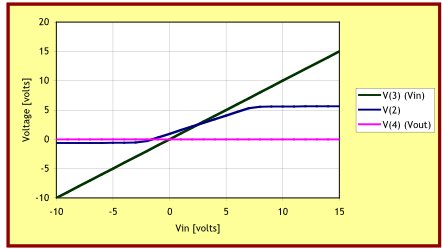
\includegraphics[width=4.5in]{clipper-dcsweep} }
\caption{DC sweep voltages at Vin, node 2 and Vout.\label{Clipper_DCSweep2}}
\end{centering}
\end{figure}

\subsection{OP Analysis}
\label{OP_Analysis}
\index{\texttt{.OP}}
\index{DC sweep!OP Analysis}
\index{OP analysis}

\Xyce{} also supports \texttt{.OP} analysis statements.  In \Xyce{},
consider \texttt{.OP} as a shorthand for a single-step DC sweep, in
which all the default operating point values are used.  One may also
consider \texttt{.OP} analysis to be the operating point calculation
that would occur as the initial step to a transient calculation,
without the subsequent time steps.

This capability was mainly added to enable the code to handle legacy
netlists using this analysis statement type.  In most versions of
SPICE, using \texttt{.OP} results in extra output not available from a
DC sweep.  \Xyce{} will also output some of this extra information about
devices, but the capability is not fully implemented.

\subsection{Output}
\label{DC_Output}\index{\texttt{.PRINT}!\texttt{DC}}

During analysis a number of output files may be generated.  The
selection of which files are created depends on a variety of factors,
most obvious of which is the \texttt{.PRINT} command.
Table~\ref{DC_Output_table} lists the format options and files created.
The column labeled ``Additional Columns'' lists the additional data that
is written, though not specified on the \texttt{.PRINT} line.

\begin{table}[htbp]
  \caption{Output generated for DC analysis \label{DC_Output_table}}
  \begin{tabularx}{\linewidth}{|p{2.75in}|Y|Y|}
    \rowcolor{XyceDarkBlue} \color{white}\textbf{Command} & \color{white}\textbf{Files} & \color{white}\textbf{Additional Columns} \\ \hline
\texttt{.PRINT DC} & \emph{circuit-file}.prn & INDEX TIME \\ \hline
\texttt{.PRINT DC FORMAT=NOINDEX} & \emph{circuit-file}.prn & TIME \\ \hline
\texttt{.PRINT DC FORMAT=CSV} & \emph{circuit-file}.csv & TIME \\ \hline
\texttt{.PRINT DC FORMAT=RAW} & \emph{circuit-file}.raw & TIME \\ \hline
\texttt{.PRINT DC FORMAT=TECPLOT} & \emph{circuit-file}.dat & TIME \\ \hline
\texttt{.PRINT DC FORMAT=PROBE} & \emph{circuit-file}.csd & TIME \\ \hline

\texttt{\emph{Xyce} -r} & \emph{circuit-file}.raw & All circuit variables printed \\ \hline
\texttt{\emph{Xyce} -r -a} & \emph{circuit-file}.raw & All circuit variables printed \\ \hline

\texttt{.OP} & \emph{log-file} & Operating point information \\ \hline

  \end{tabularx}
%% \index{sources!time-dependent}
\end{table}





%%%%%%
% -------------------------------------------------------------------------
% Transient Analysis Section ----------------------------------------------
% -------------------------------------------------------------------------
%\clearpage
\section{Transient Analysis}
\label{Trans_Overview}
\label{Transient_Analysis}
\index{analysis!transient} \index{transient analysis}
\index{\texttt{.TRAN}}

The transient response analysis simulates the response of the circuit
from \texttt{TIME=0} to a specified time.  Throughout a transient
analysis, any or all of the independent sources may have
time-dependent values.

In \Xyce{} (and most other circuit simulators), the transient analysis
begins by performing its own bias point\index{bias point} calculation
at the beginning of the run, using the same method as used for DC
sweep. This is required to set the initial conditions for the
transient solution as the initial values of the sources may differ
from their DC values.

\subsection{.TRAN Statement}

To run a transient simulation, the circuit netlist file must contain a
\verb|.TRAN| command.

\Example{\\
\texttt{ .TRAN 100us 300ms } \\
\texttt{ .TRAN 100p 12.05u 9.95u }
}

The \Xyce{} Reference Guide\ReferenceGuide{} provides a detailed
explanation of the \verb|.TRAN| statement. The netlist must also
contain one of the following:

\begin{XyceItemize}
\item Independent, transient source (see table~\ref{Time_Sources}),
\item Initial condition on a reactive element, or
\item Time-dependent analog behavioral modeling source (see chapter~\ref{Behavioral_Modeling})
\end{XyceItemize}

\subsection{Defining a Time-Dependent (transient) Source}
\label{Defining_Source}
\index{sources!defining time-dependent}

\subsubsection{Overview of Source Elements}

Source\index{sources} elements, either voltage or current, are entered
in the netlist\index{netlist!sources} file as described in the \Xyce{}
Reference Guide\ReferenceGuide{}.  Table~\ref{Time_Sources} lists the
time-dependent sources available in \Xyce{} for either voltage or
current.  For voltage sources, the name is preceded by \texttt{V} while
current sources are preceded by \texttt{I}.

\begin{table}[htbp]
  \caption{Summary of \Xyce{}-supported time-dependent sources \label{Time_Sources}}
  \begin{tabularx}{\linewidth}{|Y|Y|}
    \rowcolor{XyceDarkBlue} \color{white}\bf Source Element Name &
    \color{white}\bf Description \\ \hline

    EXP & Exponential Waveform \\ \hline
    PAT & Pattern Waveform \\ \hline
    PULSE & Pulse Waveform \\ \hline
    PWL & Piecewise Linear Waveform \\ \hline
    SFFM & Frequency-modulated Waveform \\ \hline
    SIN & Sinusoidal Waveform \\ \hline

  \end{tabularx}
\index{sources!time-dependent}
\end{table}

To use time-dependent or transient sources, place the source element
line in the netlist and characterize the transient behavior using the
appropriate parameters.  Each transient source element has a separate
set of parameters dependent on its transient behavior.  In this way,
the user can create analog sources that produce sine wave, square
pulse, exponential pulse, single-frequency FM, and piecewise linear
(PWL) waveforms.

\subsubsection{Defining Transient Sources}

To define a transient source, select one of the supported sources:
independent voltage or current, choose a transient source type from
table~\ref{Time_Sources}, and provide the transient parameters (refer
to the \Xyce{} Reference Guide\ReferenceGuide{} to fully define the
source).

The following example of an independent sinusoidal voltage source in a
circuit netlist creates a voltage source between nodes 1 and 5
that oscillates sinusoidally between -5V and +5V with a frequency of
50 KHz.  The arguments specify an offset of -5V, a 10V amplitude, and
a 50KHz frequency, in that order.

\Example{\texttt{Vexample 1 5 SIN(-5V 10V 50K)}}


\subsection{Transient Time Steps}
\label{Time_Steps}
\index{solvers!transient} \index{time step!size}

During the simulation, \Xyce{} uses a calculated time step that is
continuously adjusted for accuracy and efficiency
(see~\cite{WKHH:2000} and ~\cite{Petzold:1996}).  Calculation time
step increases during periods of circuit idleness, and decreases
during dynamic portions of the waveform.  \index{time step!maximum
  size} Users may control the maximum internal step size by specifying
the step's ceiling value in the \verb|.TRAN| command (see the \Xyce{}
Reference Guide\ReferenceGuide{}).

The internal calculation time steps used might not be consistent with
the user-requested \index{output!time values} output time steps.  By
default, \Xyce{} outputs solution results at every time step it
calculates.  If the user selects output timesteps via the
\verb|.OPTIONS OUTPUT| statement (see chapter~\ref{Output}), then
\Xyce{} will output results at the interval requested, interpolating
solution variables to desired output times if necessary.


\subsection{Time Integration Methods}
\label{TransientControls}
\index{solvers!transient} \index{time step!size}

For a transient analysis, several time integration methods can be
selected to solve the circuit model's differential algebraic
equations.  The following algorithms are available:

\begin{XyceItemize}
\item Variable order Trapezoidal (combines Trapezoidal and Backward Euler) 
\item Gear method, orders 1-2.
\end{XyceItemize}




You can set the \verb|method|, \verb|maxord| and \verb|minord|
parameters to select the time integration methods via a .OPTIONS
line. The following table shows the possible settings for those three
parameters. (Note: Consult the \Xyce{} Reference Guide\ReferenceGuide
for the exact syntax of the .OPTIONS line for each time integration
method.) The default time integration method in \Xyce{} is Trap, which
is the same as SPICE, PSpice and HSPICE.

\begin{table}[htbp]
  \caption{Summary of \Xyce{}-supported time integration methods \label{Time_integration}}
  \begin{tabularx}{\linewidth}{|Y|Y|Y|}
    \rowcolor{XyceDarkBlue} \color{white}\bf  Integration Methods &
    \color{white}\bf  Option Settings & \color{white}\bf Comments \\ \hline
    Backward-Euler & method=trap maxord=1 & Backward-Euler only \\ \hline
    Trap & method=trap & combines Trapezoidal and Backward Euler (default) \\ \hline
    Trap only & method=trap minord=2 & Trapezoidal only \\ \hline
    Gear &  method=gear &  combines Backward Euler and 2nd order Gear \\ \hline
    Gear2 only &  method=gear minord=2 & 2nd order Gear only  \\ \hline
  \end{tabularx}
\index{Time integration!integration method}
\index{\texttt{.OPTIONS}!\texttt{TIMEINT}!\texttt{METHOD}} \index{\texttt{.OPTIONS}!\texttt{TIMEINT}!\texttt{MINORD}} 
\end{table}



The Trapezoidal method is often the preferred method because it is
accurate and fast.  However, this method can exhibit artificial
point-to-point ringing, which can be controlled by using tighter
tolerances. If a circuit fails to converge with the Trapezoidal method
then you can re-run the transient analysis using the Gear method.

The Gear method may help convergence for some circuits. The 2nd order
Gear method is typically more accurate than the Backward-Euler method
(1st order Gear). However, both of these methods are overly stable
methods, and they can damp the actual circuit behavior when simulating
high-Q resonators such as oscillators.  The Backward-Euler method has
more damping effect than the 2nd order Gear method.  This effect can
be alleviated by using tighter tolerances in the simulations. However,
it is suggested to use the pure Trapezoidal method for oscillators.

\subsection{Error Controls}
\label{Time_Step_Selection}
\index{solvers!transient} \index{time step!size} \index{time step!how to select}

There are two basic time-step error control methods in \Xyce{} ---
Local Truncation Error (LTE) based and non-LTE based.


\subsubsection{Local Truncation Error (LTE) Strategy}
\index{\texttt{.OPTIONS}!\texttt{TIMEINT}!\texttt{RELTOL}} \index{\texttt{.OPTIONS}!\texttt{TIMEINT}!\texttt{ABSTOL}}

All time integration methods use the LTE-based strategy by
default. The accuracy of the simulation can be controlled by
specifying appropriate relative and absolute error tolerances (RELTOL
and ABSTOL).

\Example{\\
\texttt{ .OPTIONS TIMEINT RELTOL=1e-4 ABSTOL=1e-8 } \\
}

The total tolerance of LTE is
{\\
\texttt{ $Tol_{LTE}$  = abstol +  reltol*ref}  
}

The parameter \verb|ref| is the reference value that the relative
error is compared to. It can be controlled by setting \verb|newlte|
option.

\index{\texttt{.OPTIONS}!\texttt{TIMEINT}!\texttt{NEWLTE}}
\Example{\\
\texttt{ .OPTIONS TIMEINT NEWLTE=1 } \\
}

The  choices for \verb|newlte| option are:

\begin{XyceItemize} 
\item 0. The reference value is the current value on each node. This is the most conservative and least used.
\item 1. The reference value is the maximum of all the signals at the current time. This is the default value.
\item 2. The reference value is the maximum of all the signals over all past time. This is the loosest criterion. It normally produces the best performance and should be used if the overall size of the signals is roughly the same on all nodes.
\item 3. The reference value is the maximum value on each signal over all past time. This should be used if the scale of signals varies widely in a system.
\end{XyceItemize}

The Trapezoid integrator algorithm introduces no numerical
dissipation.  So, a strong ringing (artificially introduced by the
numerical algorithm) will occur when sources or models introduce
discontinuities.  This can result in a large local truncation error
estimate, ultimately leading to a ``time-step too small'' error.  In
this case, using the Gear method or a non-LTE strategy may help.

\subsubsection{Non-LTE Strategy}
The non-LTE strategy used in \Xyce{} is based on success of the
nonlinear solve, and is enabled by setting ERROPTION=1.  Since the
step-size selection is based only upon nonlinear iteration statistics
rather than accuracy, it is highly suggested that DELMAX be specified,
in a circuit-specific manner, for all three time integrators.  The
purpose of DELMAX is to limit the largest time step taken.

\Example{\\
\texttt{ .OPTIONS TIMEINT ERROPTION=1 DELMAX=1.0e-4 } \\
}

For the Trapezoid and Gear integrators, the options are slightly more
refined.  If the number of nonlinear iterations is below NLMIN, then
the step size is doubled. If the number of nonlinear iterations is
above NLMAX then the step size is cut by one eighth.  In between, the
step size is not changed.  An example using Trap (METHOD=7) is given
below.  \index{\texttt{.OPTIONS}!\texttt{TIMEINT}!\texttt{NLMIN}}
\index{\texttt{.OPTIONS}!\texttt{TIMEINT}!\texttt{NLMAX}}
\index{\texttt{.OPTIONS}!\texttt{TIMEINT}!\texttt{DELMAX}}

\Example{\\
\texttt{ .OPTIONS TIMEINT METHOD=7 ERROPTION=1 NLMIN=3 NLMAX=8 DELMAX=1.0e-4 } \\
}

If the number of Newton iterations is bigger than NLmax and
TIMESTEPSREVERSAL is not set, then \Xyce{} will cut the next step.  If
the number of Newton iterations is bigger than NLmax and
TIMESTEPSREVERSAL is set, then \Xyce{} will reject the current step
and also cut the current step.

\Example{\\
\texttt{ .OPTIONS TIMEINT METHOD=7 ERROPTION=1 DELMAX=1.0e-4 TIMESTEPSREVERSAL=1 } \\
}

\subsection{Breakpoints}

\index{\texttt{.OPTIONS}!\texttt{TIMEINT}!\texttt{BREAKPOINTS}} 

It is often necessary or desirable for the time integrator to be
forced to land on a specific time point and restart integration from
that point.  The most common scenario for which this is necessary is
when an device (such as a \texttt{PULSE} or a \texttt{PWL} source)
produces a discontinuity.  If a discontinuity is present, and no
breakpoint is set, then the LTE analysis will force the time
integrator to take really small time steps, and this can possibly
impact the robustness of the calculation.

Fortunately, \Xyce{} handles most device-based discontinuities
automatically, so it is not necessary for the user to worry about
them.  However, it can be desirable for the user to manually set
breakpoints from the netlist.  In a \Xyce{} netlist, these are
specified using the BREAKPOINTS parameter with a comma-separated list
in the following \texttt{.OPTIONS TIMEINT} statement.

\Example{\\
\texttt{ .OPTIONS TIMEINT BREAKPOINTS=1ms,2ms,3ms} \\
}

\subsection{Checkpointing and Restarting}
\label{Restart}
\index{checkpoint} \index{restart}

\Xyce{} was designed to simulate large, complex circuits over long
simulation runs.  Because complex simulations can take many hours (or
even days) to complete, it can sometimes be helpful to use
``checkpointing.''  When checkpointing is used, \Xyce{} periodically
saves its complete simulation state.  The saved state can be used to
restart \Xyce{} from one of these ``checkpoints.''  In the event of a
computer crash, power outage, or should the simulation need to be
interrupted for some other reason, checkpointing allows the user to
restart a long simulation in the middle of a run without having to
start over.

\Xyce{} uses the \index{netlist!restart} \index{\texttt{.OPTIONS}!\texttt{RESTART}} \verb|.OPTIONS RESTART|
netlist command to control all checkpoint output and restarting.  

\subsubsection{Checkpointing Command Format}
\index{checkpoint!format} \index{restart!format} \index{\texttt{.OPTIONS}!\texttt{RESTART}}

\begin{XyceItemize}
\item \verb+.OPTIONS RESTART [PACK=<0|1>] JOB=<job name> INITIAL_INTERVAL=<interval>+ \\
  \verb+[[<t0> <i0> [<t1> <i1>...]]]+

  \texttt{PACK=<0|1>} indicates whether restart data files will contain byte-packed (binary) data(\texttt{PACK=1}, the default) or unpacked (ASCII)(\texttt{PACK=0}).
  \texttt{JOB=<job name>} identifies the prefix for restart files.  The actual restart files will be the job name appended with the current simulation time (e.g., \texttt{name1e-05} for \texttt{JOB=name} and simulation time 1e-05 seconds).  Furthermore, the\\ \texttt{INITIAL\_INTERVAL=<interval>} identifies the initial interval time used for restart output; this parameter must be given.  The \texttt{<tx ix>} intervals identify times (\texttt{tx}) at which the output interval (\texttt{ix}) will change.  This functionality is identical to that described for the \index{\texttt{.OPTIONS}!\texttt{OUTPUT}}
  \texttt{.OPTIONS OUTPUT} command (section~\ref{Output_Control}).
\item Example --- Generate checkpoints every 0.1 $\mu s$:
\begin{vquote}
.OPTIONS RESTART JOB=checkpt INITIAL_INTERVAL=0.1us
\end{vquote}
\item Example --- Generate unpacked checkpoints every 0.1 $\mu s$:
\begin{vquote}
.OPTIONS RESTART PACK=0 JOB=checkpt INITIAL_INTERVAL=0.1us
\end{vquote}
\item Example --- Initial interval of 0.1 $\mu s$, at 1 $\mu s$ in the
  simulation, change to interval of 0.5 $\mu s$, and at 10 $\mu s$ change to an
  interval of 0.1 $\mu s$:
\begin{vquote}
.OPTIONS RESTART JOB=checkpt INITIAL_INTERVAL=0.1us 1us 0.5us
+ 10us 0.1us
\end{vquote}
\end{XyceItemize}

\subsubsection{Restarting Command Format}
\index{restart!format}

\begin{XyceItemize}
\item \index{\texttt{.OPTIONS}!\texttt{RESTART}}
\verb+.OPTIONS RESTART <FILE=<filename> | JOB=<job name> START_TIME=<time>>+ \\
\verb|+ [INITIAL_INTERVAL=<interval> [<t0> <i0> [<t1> <i1> ...]]]|
\end{XyceItemize}
To restart\index{restart} from an existing restart file, specify the file by using either the\\%
\texttt{FILE=<filename>} parameter to explicitly request a file or\\%
\texttt{JOB=<job name> START\_TIME=<time>} to specify a file prefix and a
specific time.  The time must exactly match an output file time for the
simulator to correctly load the file.  

To continue checkpointing the simulation in a restarted run, append
\texttt{INITIAL\_INTERVAL=<interval>} and the following intervals to
the command in the same format as previously described.  Without these
additional parameters, the simulation will restart as requested, but
will not generate further checkpoint files.

\begin{XyceItemize}
\item Example\index{Example!restarting} --- Restart from checkpoint file at 0.133
  $\mu s$:
\begin{vquote}
.OPTIONS RESTART JOB=checkpt START_TIME=0.133us
\end{vquote}
\item Example --- Restart from checkpoint file at 0.133 $\mu s$ :
\begin{vquote}
.OPTIONS RESTART FILE=checkpt0.000000133
\end{vquote}
\item Example --- Restart from 0.133 $\mu s$ and continue checkpointing at 0.1
      $\mu s$ intervals:
\begin{vquote}
.OPTIONS RESTART FILE=checkpt0.000000133 JOB=checkpt_again
+ INITIAL_INTERVAL=0.1us
\end{vquote}
\end{XyceItemize}
\subsection{Output}
\label{Transient_Output}\index{\texttt{.PRINT}!\texttt{TRAN}}

During analysis a number of output files may be generated.  The
selection of which files are created depends on a variety of factors,
most obvious of which is the \texttt{.PRINT} command.
Table~\ref{Tran_Output_table} lists the format options and files
created.  The column labeled ``Additional Columns'' lists the additional
data that is written, though not specified on the \texttt{.PRINT} line.

\begin{table}[htbp]
  \caption{Output generated for Transient analysis \label{Tran_Output_table}}
  \begin{tabularx}{\linewidth}{|p{2.75in}|Y|Y|}
    \rowcolor{XyceDarkBlue} \color{white}\textbf{Command} & \color{white}\textbf{Files} & \color{white}\textbf{Additional Columns} \\ \hline
\texttt{.PRINT TRAN} & \emph{circuit-file}.prn & INDEX TIME \\ \hline
\texttt{.PRINT TRAN FORMAT=NOINDEX} & \emph{circuit-file}.prn & TIME \\ \hline
\texttt{.PRINT TRAN FORMAT=CSV} & \emph{circuit-file}.csv & TIME \\ \hline
\texttt{.PRINT TRAN FORMAT=RAW} & \emph{circuit-file}.raw & TIME \\ \hline
\texttt{.PRINT TRAN FORMAT=TECPLOT} & \emph{circuit-file}.dat & TIME \\ \hline
\texttt{.PRINT TRAN FORMAT=PROBE} & \emph{circuit-file}.csd & TIME \\ \hline

\texttt{\emph{Xyce} -r} & \emph{circuit-file}.raw & All circuit variables printed \\ \hline
\texttt{\emph{Xyce} -r -a} & \emph{circuit-file}.raw & All circuit variables printed \\ \hline

\texttt{.OP} & \emph{log-file} & Operating point information \\ \hline

  \end{tabularx}
%% \index{sources!time-dependent}
\end{table}

% -------------------------------------------------------------------------
% STEP Analysis Section ---------------------------------------------------
% -------------------------------------------------------------------------
\clearpage
\section{STEP Parametric Analysis}
\label{STEP_Analysis}
\label{step_Overview}
\index{analysis!STEP} \index{STEP parametric analysis}
\index{\texttt{.STEP}}

The \verb|.STEP| command performs a parametric sweep for all the
analyses of the circuit.  When the \verb|.STEP| command is invoked,
typical analyses, such as \verb|.DC|, \verb|.AC|, and \verb|.TRAN| are
performed for each value of the stepped parameter.

This capability is very similar, but not identical, to the \verb|STEP|
capability in PSpice~\cite{PSpiceUG:1998}.  \Xyce{} can use
\verb|.STEP| to sweep over any device instance or device model
parameter, as well as the circuit temperature.  It is not legal to
sweep parameters defined in \texttt{.PARAM} statements, but it is
legal to sweep global parameters defined in \texttt{.global\_param}
statements.  Section~\ref{Parameters_Expressions}) discusses these two
distinct parameter definitions.

\subsection{.STEP Statement}

A \verb|.STEP| analysis may be specified by simply adding a
\verb|.STEP| line to a netlist.  Unlike \verb|.DC|, \verb|.STEP| by
itself is not an adequate analysis specification, as it merely
specifies an outer loop around the normal analysis.  A standard
analysis line, either specifying \verb|.TRAN|, \verb|.AC| and
\verb|.DC| analysis, is still required.

Some examples of typical \verb|.STEP| lines are:

\Example{\\
\texttt{ .STEP M1:L  7u 5u -1u } \\
\texttt{ .STEP OCT V0 0.125 64 2 } \\
\texttt{ .STEP DEC R1 100 10000 3 } \\
\texttt{ .STEP TEMP LIST 10.0 15.0 18.0 27.0 33.0 } \\
\texttt{ .STEP data=table }
}

\verb|.STEP| has a format similar to that of the \verb|.DC| format
specification.  In the first example, \verb|M1:L| is the name of the
parameter (in this instance, the length parameter of the MOSFET
\texttt{M1}), \verb|7u| is the initial value of the parameter,
\verb|5u| is the final value of the parameter, and \verb|-1u| is the
step size.  Like \verb|.DC|, \verb|.STEP| in \Xyce{} can also handle
sweeps by decade, octave, a specified lists of values, or multivariate parameter values from a table.  Consult the
\Xyce{} Reference Guide\ReferenceGuide{} for complete explanations of each sweep type.

\subsection{Sweeping over a Device Instance Parameter}
\label{step_InstanceParam}

The first example uses \verb|M1:L| as the parameter, but it could have
used any model or instance parameter existing in the
circuit. Internally, \Xyce{} handles the parameters for all device
models and device instances in the same way.  Users can uniquely
identify any parameter by specifying the device instance name,
followed by a colon (:), followed by the specific parameter name.  For
example, all the MOSFET models have an instance parameter for the
channel length, L.  For a MOSFET instance specified in a netlist,
named M1, the full name for the M1 channel length parameter is M1:L.

Figure~\ref{Step_Netlist_1} provides a simple application of
\verb|.STEP| to a device instance.  This is the same diode clipper
circuit as was used in the transient analysis chapter, except that a
single line (in red) has been added.  This \verb|.STEP| line will
cause \Xyce{} to sweep the resistance of the resistor, R4, from 3.0
KOhms to 15.0 KOhms, in 2.0 KOhms increments, meaning seven transient
simulations will be performed, each one with a different value for R4.

As the circuit is executed multiple times, the resulting output file
is a little more sophisticated.  The \verb|.PRINT| statement is still
used in much the same way as before.  However, the .prn output file
contains the concatenated output of each \verb|.STEP| increment.  The
end of this section provides more details of how \texttt{.STEP}
changes output files.

\begin{figure}[htbp]
\begin{centering}
\shadowbox{
\begin{minipage}{0.8\textwidth}
\begin{vquote}

Transient Diode Clipper Circuit with Step Analysis
* Voltage Sources
VCC 1 0 5V
VIN 3 0 SIN(0V 10V 1kHz)\color{black}
* Analysis Command
.TRAN 2ns 2ms\color{black}
* Output
.PRINT TRAN V(3) V(2) V(4)\color{black}
\color{XyceRed} * Step statement \color{black}
\color{XyceRed}.STEP R4:R 3.0K 15.0K 2.0K \color{black}
* Diodes
D1 2 1 D1N3940
D2 0 2 D1N3940
* Resistors
R1 2 3 1K
R2 1 2 3.3K
R3 2 0 3.3K
R4 4 0 5.6K
* Capacitor
C1 2 4 0.47u
.MODEL D1N3940 D(
+ IS=4E-10 RS=.105 N=1.48 TT=8E-7
+ CJO=1.95E-11 VJ=.4 M=.38 EG=1.36
+ XTI=-8 KF=0 AF=1 FC=.9
+ BV=600 IBV=1E-4)
.END
\end{vquote}
\end{minipage}
}
\caption{Diode clipper circuit netlist for step transient
analysis\label{Step_Netlist_1}}
\end{centering}
\end{figure}

\subsection{Sweeping over a Device Model Parameter}
\label{step_ModelParam}

Sweeping a model parameter can be done in an identical manner to an
instance parameter.  Figure~\ref{Step_Netlist_2} contains the same
circuit as in figure~\ref{Step_Netlist_1}, but with additional
\verb|.STEP| line referring to a model parameter, \verb|D1N3940:IS|.

NOTE: \verb|.STEP| line syntax differs from \verb|.DC| line syntax in
that multiple parameters require separate \verb|.STEP| lines. Each
parameter needs a separate line.

\begin{figure}[htbp]
\begin{centering}
\shadowbox{
\begin{minipage}{0.8\textwidth}
\begin{vquote}

Transient Diode Clipper Circuit with Step Analysis
* Voltage Sources
VCC 1 0 5V
VIN 3 0 SIN(0V 10V 1kHz)\color{black}
* Analysis Command
.TRAN 2ns 2ms\color{black}
* Output
.PRINT TRAN V(3) V(2) V(4)\color{black}
\color{XyceRed} * Step statements \color{black}
\color{XyceRed}.STEP R4:R 3.0K 15.0K 2.0K \color{black}
\color{XyceRed}.STEP D1N3940:IS 2.0e-10 6.0e-10 2.0e-10 \color{black}
* Diodes
D1 2 1 D1N3940
D2 0 2 D1N3940
* Resistors
R1 2 3 1K
R2 1 2 3.3K
R3 2 0 3.3K
R4 4 0 5.6K
* Capacitor
C1 2 4 0.47u
.MODEL D1N3940 D(
+ IS=4E-10 RS=.105 N=1.48 TT=8E-7
+ CJO=1.95E-11 VJ=.4 M=.38 EG=1.36
+ XTI=-8 KF=0 AF=1 FC=.9
+ BV=600 IBV=1E-4)
.END
\end{vquote}
\end{minipage}
}
\caption{Diode clipper circuit netlist for 2-step transient
analysis\label{Step_Netlist_2}}
\end{centering}
\end{figure}

\subsection{Sweeping over Temperature}
\label{step_Temperature}

It is also possible to sweep over temperature.  To do so, simply
specify \verb|temp| as the parameter name.  It will work in the same
manner as \verb|.STEP| when applied to model and instance parameters.

\subsection{Special cases: Sweeping Independent Sources, Resistors, Capacitors and Inductors}
\label{step_SpecialCases}

For some devices, there is generally only one parameter that one would
want to sweep.  For example, a linear resistor's only parameter of
interest is resistance, R.  Similarly, for a DC voltage or current
source, one is usually only interested in the magnitude of the source,
DCV0.  Finally, linear capacitors generally only have capacitance, C,
as a parameter of interest, while inductors generally only have
inductance, L, as a parameter of interest.

For these simple devices, it is not necessary to specify both the
parameter and device on the \texttt{.STEP} line: only the device name
is strictly required, as these devices have default parameters that
are assumed if no parameter name is given explicitly.

Examples of usage are given below.  The first two lines are equivalent
--- in the first line, the resistance parameter of \texttt{R4} is
named explicitly, and in the second line the resistance parameter is
implicit. A similar example is then shown for the DC voltage of the
voltage source \texttt{VCC}.  In the remaining lines, parameter names
are all implicit, and the default parameters of the associated devices
are used.

\Example{ \\
\begin{tabular}{lllll}
  \texttt{.STEP R4:R} &\texttt{3.0K}  &\texttt{15.0K}  &\texttt{2.0K} \\ 
  \texttt{.STEP R4} &\texttt{3.0K}  &\texttt{15.0K}  &\texttt{2.0K} \\
  \texttt{.STEP VCC:DCV0}&\texttt{4.0 }  &\texttt{ 6.0 }  &\texttt{1.0 } \\  
  \texttt{.STEP VCC}&\texttt{4.0 }  &\texttt{ 6.0 }  &\texttt{1.0 } \\ 
  \texttt{.STEP ICC}&\texttt{4.0 }  &\texttt{ 6.0 }  &\texttt{1.0 } \\ 
  \texttt{.STEP C1} &\texttt{0.45u} &\texttt{ 0.50u} &\texttt{0.1u} \\
  \texttt{.STEP L1} &\texttt{0.5m} &\texttt{ 1.0m} &\texttt{0.5m} \\
\end{tabular}
        }

Independent sources require further explanation.  Their default
parameter, DCV0, only applies to \texttt{.DC} analyses.  They do not have
default parameters for their transient forms, such as \texttt{SIN}
or \texttt{PULSE}.

\subsection{Output files}
\label{step_output_files}
\index{output!\texttt{.STEP}}

Users can think of \texttt{.STEP} simulations as several distinct
executions of the same circuit netlist.  The output data, as specified
by a \texttt{.PRINT} line, however, goes to a single (\texttt{*.prn})
file.  For convenience, \Xyce{} also creates a second auxilliary file
with the \texttt{*.res} suffix.

Figure~\ref{Step_Netlist_1} shows an example file named
\verb+clip.cir+, which when run will produce files \verb+clip.cir.res+
and \verb+clip.cir.prn+.  The file \verb+clip.cir.res+ contains one
line for each step, showing what parameter value was used on that
step.  \verb+clip.cir.prn+ is the familiar output format, but the
\verb+INDEX+ field recycles to zero each time a new step begins.  As
the default behavior distinguishes each step's output only by
recycling the \verb+INDEX+ field to zero, it can be beneficial to add
the sweep parameters to the \verb+.PRINT+ line.  For the default file
format (\texttt{format=std}), \Xyce{} will not automatically include
these sweep parameters, so for plotting it is usually best to specify
them by hand.

If using the default \texttt{.prn} file format (\texttt{format=std}),
the resulting \texttt{.STEP} simulation output file will be a simple
concatenation of each step's underlying analysis output.  If using
\texttt{format=probe}, the data for each execution of the circuit will
be in distinct sections of the file, and it should be easy to plot the
results using PROBE.  If using \texttt{format=tecplot}, the results of
each \texttt{.STEP} simulation will be in a distinct Tecplot
zone. Finally, format=raw will place the results for each
\texttt{.STEP} simulation in a distinct ``plot'' region.

% Sandia National Laboratories is a multimission laboratory managed and
% operated by National Technology & Engineering Solutions of Sandia, LLC, a
% wholly owned subsidiary of Honeywell International Inc., for the U.S.
% Department of Energy’s National Nuclear Security Administration under
% contract DE-NA0003525.

% Copyright 2002-2021 National Technology & Engineering Solutions of Sandia,
% LLC (NTESS).

% -------------------------------------------------------------------------
% Sampling Analysis Section ---------------------------------------------------
% -------------------------------------------------------------------------
\clearpage
\section{Random Sampling Analysis}
\label{SAMPLING_Analysis}
\label{sampling_Overview}
\index{analysis!Sampling} \index{Sampling analysis} \index{Random Sampling}
\index{\texttt{.SAMPLING}}
\index{\texttt{.EMBEDDEDSAMPLING}}
\Xyce{} supports two different styles of random sampling analysis.  One is specified 
with the \verb|.SAMPLING| 
command, and the other is specified with the \verb|.EMBEDDEDSAMPLING| commmand.  
These are relatively new capabilities and are still under development.  

The \verb|.SAMPLING| command causes \Xyce{} to execute the primary analysis (\verb|.DC|,
\verb|.AC|, \verb|.TRAN|, etc.) inside a loop over randomly distributed parameters.  
The user specifies a list of random parameters, their distributions, distribution 
parameters (such as mean and standard deviation), and the total number of 
sample points.  The primary analysis is then executed sequentially for each sample point.
The \verb|.SAMPLING| capability uses a lot of the same code base as \verb|.STEP|, 
so most of the guidance for \verb|.STEP|, including legal parameters, output 
file formats, supported analyses types, etc., also applies to \verb|.SAMPLING|.

The \verb|.EMBEDDEDSAMPLING| command also causes \Xyce{} to create a loop over 
randomly distributed parameters, but unlike \verb|.SAMPLING|, this loop is 
implemented inside the solver loop rather than outside of it.  As such, it 
creates a block linear system, in which each matrix block has the structure 
of the original matrix, and the number of blocks is equal to the number of sample points.
As such, all the parameters are propagated simultaneously, rather than sequentially.
Unlike \verb|.SAMPLING|, which can be applied to all types of \Xyce{} analysis, 
\verb|.EMBEDDEDSAMPLING| can only be applied to \verb|.DC| and \verb|.TRAN|.

Both types of sampling methods can be applied to a variety of inputs and outputs.
For inputs,
\Xyce{}  can use \verb|.SAMPLING| or \verb|.EMBEDDEDSAMPLING| to modify 
any device instance or device
model parameter, as well as the circuit temperature.  It can also be used 
to sweep over any user-defined parameter (either \texttt{.GLOBAL\_PARAM} 
or \texttt{.PARAM} ), as long as that parameter is  defined in the 
global scope.

For outputs, both \verb|.SAMPLING| and \verb|.EMBEDDEDSAMPLING| 
can apply statistical analysis (computing moments such as mean and standard deviation) 
to most outputs that appear on the \verb|.PRINT| line.
However, the two analysis types have some differences.    \verb|.SAMPLING| will only 
apply statistical analysis at the end of the calculation, while \verb|.EMBEDDEDSAMPLING| 
can apply statistical analysis at each time step.  Relatedly, 
\verb|.SAMPLING| can also be applied to any \verb|.MEASURE|, but 
\verb|.EMBEDDEDSAMPLING| lacks this capability. 

\subsection{.SAMPLING and .EMBEDDEDSAMPLING Statements}
\label{sampling_statement}
Sampling analysis may be specified by simply adding a \verb|.SAMPLING| 
or a \verb|.EMBEDDEDSAMPLING| line to a netlist.    The format for the two commands is nearly 
identical.

Sampling analysis such as \verb|.SAMPLING| or \verb|.EMBEDDEDSAMPLING| is not considered a ``primary'' analysis type.
This means that such a command by itself is not an 
adequate analysis specification, as it merely specifies an additional parametric loop to augment the
primary analysis.  A standard analysis line, specifying \verb|.TRAN|, \verb|.AC|, \verb|.HB|, 
and \verb|.DC| analysis, is still required.

Examples of typical \verb|.SAMPLING| lines:

\Example{\\
\texttt{\\
.SAMPLING  \\
+ param=M1:L, M1:W \\
+ type=uniform,uniform \\
+ lower\_bounds=5u,5u \\
+ upper\_bounds=7u,7u \\
}
\texttt{ \\
.SAMPLING \\
+ param=R1,c1 \\
+ type=normal,normal \\
+ means=3K,1uF \\
+ std\_deviations=1K,0.2uF \\
}

}

In the first example, \verb|M1:L| and \verb|M1:W| 
are the names of the
parameters (in this instance, the length and width parameters of the MOSFET
\texttt{M1}), \verb|5u| is the minimum value of both parameters and
\verb|7u| is the maximum value of both parameters.  For both parameters, 
the distribution (specified by \texttt{type}) is uniform.
In the second example, the two parameters are \verb|R1| and \verb|c1|.   In this 
case, it isn't necessary to specify the specific parameter of \verb|R1| or \verb|c1| 
as resistors and capacitors have simple default parameters (see section~\ref{sampling_SpecialCases}).  
The distributions of both parameters are normal, and the means and standard deviations 
are specified for both in comma-separated lists.

For any list of parameters, all the required fields must be provided in comma-separated 
lists.  \Xyce{} will throw an error if the length of any of the lists is different 
than that of the parameter list.

\subsection{.options SAMPLES and EMBEDDEDSAMPLES Statements}
\label{options_samples_statement}

To specify the number of samples, use the netlist command \texttt{.options 
SAMPLES numsamples=<value>}.   For sampling analysis to work correctly, this parameter is required.
Other sampling details, including the sampling type, the covariance matrix, 
the statistical outputs and the random seed can be specified using the 
same \verb|.options SAMPLES| netlist command.  Some examples of this command are:

\Example{\\
\texttt{ \\
.options samples numsamples=1000 \\
}
\texttt{ \\
.options samples numsamples=30 \\
+ covmatrix=1e6,1.0e-3,1.0e-3,4e-14 \\
+ OUTPUTS={R1:R},{C1:C} \\
+ MEASURES=maxSine \\
+ SAMPLE\_TYPE=LHS \\
+ SEED=743190581 \\
}
}
The random seed can be set either in the \texttt{.options SAMPLES} statement, or 
it can be set from the command line using the \texttt{-randseed} option.  If it 
is not set either way, then the random seed is generated internally.

In the example there are two different types of outputs specified.  One is using 
the keyword \texttt{OUTPUTS}, and this is used to specify a comma-separated list 
of outputs corresponding to typical \texttt{.PRINT} line outputs.  Solution 
variables, user defined parameters, and expressions depending on both are typical.  

The other type of output is specified using the keyword \texttt{MEASURES}, and 
this is used to specify a comma-separated list of netlist \texttt{.MEASURE} commands.
This type of output is only available to \texttt{.SAMPLING} and not to \texttt{.EMBEDDEDSAMPLING}.

The example sets the \texttt{SAMPLE\_TYPE=LHS}, for Latin Hypercube Sampling~\cite{HELTON200323}.  
The other options is \texttt{SAMPLE\_TYPE=MC} for Monte Carlo~\cite{Fishman1996}.  
LHS is the default option for this parameter, and will generally be a better choice.

\subsection{Specifying Uncertain Inputs}

\subsubsection{Sampling a Device Instance Parameter}
\label{sampling_InstanceParam}
Figure~\ref{Sampling_Netlist_1} provides a simple application of \verb|.SAMPLING| 
to a device instance parameter.  The circuit is a simple voltage divider driven 
by a oscillating voltage source.  The randomly sampled parameter is the resistance 
of \texttt{R1}, which is given a normal distribution with a specified mean and 
standard deviation.

As the circuit is executed multiple times, an output file is generated based on 
the \verb|.PRINT| command.  The \verb|.PRINT| statement is still used in the same 
way that it would be in a non-sampling analysis.  However, the output file 
contains the concatenated output of each \verb|.SAMPLING| step.  
Section~\ref{sampling_output_files} provides more details of how \texttt{.SAMPLING} 
changes \texttt{.PRINT} output files.

\Xyce{} computes statistical outputs for quantities specified by \texttt{OUTPUTS} 
and \texttt{MEASURES} on the \texttt{.options SAMPLES} line.  For these outputs,
moments such as mean and variance are computed and sent to standard output.  More 
details of this type of output, as well as examples, are given in section~\ref{statistical_outputs}.
\begin{figure}[htbp]
  \fontsize{9pt}{10pt}
\begin{centering}
\shadowbox{
\begin{minipage}{0.8\textwidth}
\begin{vquote}
\color{blue}Voltage Divider with sampling\color{black}
R2  1  0  7k
R1 1 2 3k
VS1  2  0  SIN(0 1.0e3 1KHZ 0 0)

.tran 0.1ms 1ms
.meas tran maxSine max V(1) 

\color{XyceRed}.SAMPLING param=R1:R 
+ type=normal means=1K std\_deviations=0.1K\color{black}

\color{XyceRed}.options SAMPLES numsamples=1000 OUTPUTS=\{R1:R\} 
+ MEASURES=maxSine SAMPLE\_TYPE=MC stdoutput=true\color{black} 

\end{vquote}
\end{minipage}
}
\caption{Voltage divider circuit netlist with sampling of a device instance parameter.
Sampling commands are in \color{XyceRed}red\color{black}.
\label{Sampling_Netlist_1}}
\end{centering}
\end{figure}

\subsubsection{Sampling a Device Model Parameter}
\label{sampling_ModelParam}

Sampling a model parameter can be done in an identical manner to an instance parameter.  
Figure~\ref{Sampling_Netlist_2} provides a simple application of \verb|.SAMPLING| to a 
device model and a device instance.  This is the same diode clipper circuit as was used 
in the Transient Analysis section (see section \ref{Transient_Analysis_Sec}), except that 
several lines of sampling commands (in red) have been added.  

The sampling commands will cause \Xyce{} to sample the model parameter, \verb|D1N3940:IS| as well as the 
resistance of the resistor, R4. Both of the parameters are randomly sampled using uniform distributions 
with specified lower and upper bounds.
\begin{figure}[htbp]
  \fontsize{9pt}{10pt}
\begin{centering}
\shadowbox{
\begin{minipage}{0.8\textwidth}
\begin{vquote}
\color{blue}Transient Diode Clipper with Sampling Analysis\color{black}

\color{blue}* Primary Analysis Command\color{black}
.tran 2ns 0.5ms
\color{blue}* Output\color{black}
.print tran format=tecplot V(3) V(2) V(4)
.meas tran maxSine max V(4) 

\color{XyceRed}* Sampling statements 
.SAMPLING
+ param=R4:R,D1N3940:IS
+ type=uniform,uniform
+ lower\_bounds=3.0k,2.0e-10
+ upper\_bounds=15.0k,6.0e-10

.options SAMPLES numsamples=10 SAMPLE\_TYPE=LHS
+ OUTPUTS={R4:R},{D1N3940:IS} MEASURES=maxSine stdoutput=true\color{black}
\color{blue}* Voltage Sources\color{black}
VCC 1 0 5V
VIN 3 0 SIN(0V 10V 1kHz)
\color{blue}* Diodes\color{black}
D1 2 1 D1N3940
D2 0 2 D1N3940
\color{blue}* Resistors\color{black}
R1 2 3 1K
R2 1 2 3.3K
R3 2 0 3.3K
R4 4 0 5.6K
\color{blue}* Capacitor\color{black}
C1 2 4 0.47u
.MODEL D1N3940 D(
+ IS=4E-10 RS=.105 N=1.48 TT=8E-7
+ CJO=1.95E-11 VJ=.4 M=.38 EG=1.36
+ XTI=-8 KF=0 AF=1 FC=.9 BV=600 IBV=1E-4)
.END
\end{vquote}
\end{minipage}
}
\caption{Diode clipper circuit netlist with sampling analysis.  This example uses a model parameter as one of the sampling parameters.
Sampling commands are in \color{XyceRed}red\color{black}.
  \label{Sampling_Netlist_2}}
\end{centering}
\end{figure}

\subsubsection{Sampling a User-Defined Parameter}
\label{sampling_GlobalParam}

Sampling can be applied to user-defined parameters, as long as they are declared in the top level netlist (global scope).  
It cannot be applied to user-defined parameters which are defined in a subcircuit.  An example of such usage, with a global parameter, is given 
in figure~\ref{Sampling_Netlist_3}. This circuit identical to the circuit in 
figure~\ref{Sampling_Netlist_1}, except that it uses global parameters.  
If the global parameters in this netlist are changed to normal parameters (\texttt{.PARAM}), this circuit will also work.
\begin{figure}[htbp]
  \fontsize{9pt}{10pt}
\begin{centering}
\shadowbox{
\begin{minipage}{0.8\textwidth}
\begin{vquote}
\color{blue}Voltage Divider, sampling global params\color{black}
.global\_param Vmax=1000.0
.global\_param testNorm=1.5k
.global\_param R1value=\{testNorm*2.0\}

R2  1  0  7k
R1 1 2 \{R1value\}
VS1  2  0  SIN(0 \{Vmax\} 1KHZ 0 0)
.tran 0.1ms 1ms
.meas tran maxSine max V(1) 

\color{XyceRed}.SAMPLING param=testNorm
+ type=normal means=0.5K std\_deviations=0.05K\color{black}

\color{XyceRed}.options SAMPLES numsamples=1000 SAMPLE\_TYPE=MC
+ OUTPUTS=\{R1:R\} MEASURES=maxSine\color{black}

\end{vquote}
\end{minipage}
}
\caption{Voltage divider circuit netlist with sampling of a global parameter.
  Sampling commands are in \color{XyceRed}red\color{black}.  This circuit will also work if the \texttt{.global\_param} statements are changed to \texttt{.param}.
\label{Sampling_Netlist_3}}
\end{centering}
\end{figure}

\subsubsection{Sampling over Temperature}
\label{sampling_Temperature}

It is also possible to sample temperature.  To do so, simply 
specify \verb|temp| as the parameter name.  It will work in the 
same manner as \verb|.SAMPLING| when applied to model and instance 
parameters.

\subsubsection{Special cases: Sampling Independent Sources, Resistors, Capacitors and Inductors}
\label{sampling_SpecialCases}

For some devices, there is generally only one parameter that one would
want to sample.  For example, a linear resistor's only parameter of
interest is resistance, R.  Similarly, for a DC voltage or current
source, one is usually only interested in the magnitude of the source, DCV0.
Finally, linear capacitors generally only have capacitance, C, as a 
parameter of interest, while inductors generally only have inductance, L,
as a parameter of interest.  

For these simple devices, it is not necessary to specify both the
parameter and device on the \texttt{.SAMPLING} line: only the device name
is strictly required, as these devices have default
parameters that are assumed if no parameter name is given explicitly.

Examples of usage are given below.  The first two lines are equivalent
--- in the first line, the resistance parameter of \texttt{R4} is
named explicitly, and in the second line the resistance parameter is
implicit. A similar example is then shown for the DC voltage of the 
voltage source \texttt{VCC}.  In the remaining lines, parameter names are all 
implicit, and the default parameters of the associated devices are used.

\Example{ \\
          \fontsize{10pt}{11pt}
\begin{tabular}{lllll}
  \texttt{.SAMPLING param=R4:R,C1:C} &\texttt{type=normal,normal}  &\texttt{means=3k,1u}  &\texttt{std\_deviations=1k,0.1u} \\ 
  \texttt{.SAMPLING param=R4,C1} &\texttt{type=normal,normal}  &\texttt{means=3k,1u}  &\texttt{std\_deviations=1k,0.1u} \\ 
  \texttt{.SAMPLING VCC:DCV0}&\texttt{type=uniform}  &\texttt{means=6.0}  &\texttt{std\_deviations=1.0 } \\  
  \texttt{.SAMPLING VCC}&\texttt{type=uniform}  &\texttt{means=6.0}  &\texttt{std\_deviations=1.0 } \\ 
  \texttt{.SAMPLING param=C1} &\texttt{type=normal}  &\texttt{means=0.5u}  &\texttt{std\_deviations=0.05u} \\ 
  \texttt{.SAMPLING param=L1} &\texttt{type=normal}  &\texttt{means=0.5m}  &\texttt{std\_deviations=0.01m} \\ 
\end{tabular}
        }

Independent sources require further explanation.  Their default
parameter, DCV0, only applies to \texttt{.DC} analyses.  They do not have
default parameters for their transient forms, such as \texttt{SIN}
or \texttt{PULSE}.

\subsubsection{Sampling using random operators from expressions}

The \Xyce{} expression library supports random operators in expressions, 
including \texttt{AGAUSS}, \texttt{GAUSS}, \texttt{AUNIF}, \texttt{UNIF} and \texttt{RAND}.
\Xyce{} \texttt{.SAMPLING} and \texttt{.EMBEDDEDSAMPLING} analyses are able to use these, but they are not
connected by default.  In order to use random expression operators with \texttt{.SAMPLING}, 
the following commend must be present in the netlist:

\Example{\\
\texttt{\\
.SAMPLING  useExpr=true
}
}
This capability is potentially very powerful, as the random operators can 
act as operators within complex expressions.  
As expressions can be applied to \texttt{.param}, \texttt{.global\_param}, 
device instance parameters  and device model parameters, this capability 
naturally can be applied to any of these types of input parameters.
A simple example of this feature, applied to several instance parameters, 
can be seen in figure~\ref{Sampling_Netlist_4}.  Other examples of this capability can be found 
in the netlists given in figures~\ref{regressionPCE_Netlist1},~\ref{NISP_netlist1} 
and~\ref{NISP_gilbert_netlist}.

This feature cannot be used in the same netlist as the 
specification described in section~\ref{sampling_statement}.  If 
\texttt{useExpr=true}, \Xyce{} will ignore the comma-separated lists such as 
\texttt{param}.  Likewise, if \texttt{useExpr=false} (the default), then 
\Xyce{} will not randomly sample any random operators present in the circuit.  
It will only sample the parameters listed by comma-separated lists.

\begin{figure}[htbp]
  \fontsize{9pt}{10pt}
\begin{centering}
\shadowbox{
\begin{minipage}{0.8\textwidth}
\begin{vquote}
\color{blue}sampling example with random expression operators \color{black}
R4 b 0 \{agauss(4k,0.4k,1)\}
R3 a b \{agauss(1k,0.1k,1)\}
R2 1 a \{agauss(2k,0.2k,1)\}
R1 1 2 \{agauss(3k,0.1k,1)\}
v1 2 0 10V

.dc v1 10 10 1
.print dc v(1)

.SAMPLING 
+ useExpr=true

.options SAMPLES numsamples=10
+ outputs=\{v(1)\}
+ sample\_type=lhs
+ stdoutput=true
.end

\end{vquote}
\end{minipage}
}
\caption{Voltage divider circuit netlist using random expression operators.
\label{Sampling_Netlist_4}}
\end{centering}
\end{figure}

\subsection{Output files}
\label{sampling_output_files}

The two types of sampling produce different types of output files.  This is 
related to the fact that for \texttt{.SAMPLING} the calculations for each sample 
point are performed sequentially, while for \texttt{.EMBEDDEDSAMPLING} the 
calculations for each sample point are performed simultaneously.  As such, 
for \texttt{.SAMPLING} statistical moments can only be computed at the end 
of the calculation, once all the sample points are avaible.  In contrast, 
for \texttt{.EMBEDDEDSAMPLING}, statistical moments can be computed throughout 
the calculation, as all the sample points are available for each step.

\subsubsection{\texttt{.SAMPLING} output files}
\index{output!\texttt{.SAMPLING}}
Users can think of \texttt{.SAMPLING} simulations as being very similar 
to \texttt{.STEP} and thus comprised of a sequential set of distinct executions
of the same circuit netlist. The main difference is the source of the specific sample points.

Similar to \texttt{.STEP}, the output data can be requested by a standard \texttt{.PRINT} command, for the underlying primary analsis.
For example, if applying \texttt{.SAMPLING} to a transient analysis, then the appropriate \texttt{.PRINT} command will be \texttt{.PRINT TRAN}.
The output data will go to a single file, with each sample point in a different section of the output file.
If using the default \texttt{.prn} file format (\texttt{format=std}), the 
resulting \texttt{.SAMPLING} simulation output file will be a simple concatenation of
each step's underlying analysis output.
If using \texttt{format=probe}, the data for each execution of the circuit
will be in distinct sections of the file, and it should be easy to 
plot the results using PROBE.  If using \texttt{format=tecplot}, 
the results of each \texttt{.SAMPLING} simulation will be in a distinct
Tecplot zone. Finally, format=raw will place the results for each \texttt{.SAMPLING} 
simulation in a distinct ``plot'' region. 

Another similarity to \texttt{.STEP} is that \Xyce{} creates a second auxilliary file with the \texttt{*.res} 
suffix, which contains the parameter values.    This can be useful for seeing the exact sampling parameter values in a compact file.

Statistical outputs can also be produced (see section~\ref{statistical_outputs}) 
for \texttt{.SAMPLING} in the form of moments, but these can only be computed 
at the end of the calculation once all the samples are available.  These statistical outputs will not
be present in the \texttt{.PRINT} specified output file, since it is output on-the-fly.

Figure~\ref{Sampling_Netlist_2} shows an example file named \verb+clip.cir+, which when run will produce files
\verb+clip.cir.res+ and \verb+clip.cir.prn+.  The file \verb+clip.cir.res+
contains one line for each step, showing what parameter value was used
on that step.  \verb+clip.cir.prn+ is the familiar output format, but
the \verb+INDEX+ field recycles to zero each time a new step begins.
As the default behavior distinguishes each step's output only by recycling 
the \verb+INDEX+ field to zero, it can be beneficial to add the sampling
parameters to the \verb+.PRINT+ line.   For the default file format 
(\texttt{format=std}), \Xyce{} will not automatically include these sampling parameters,
so for plotting it is usually best to specify them by hand.


Note that for sampling calculations involving a really large number of sample 
points, the single output file can become prohibitively large.  Be careful when 
using \verb|.PRINT| if the number of samples is large.   If the number is really 
large (thousands) consider excluding any \verb|.PRINT| output statements and 
just rely on statistical outputs, described next in section~\ref{statistical_outputs}.
Similarly, the generation of the measure output can be suppressed with 
\texttt{.OPTIONS MEASURE MEASPRINT}.

\subsubsection{\texttt{.EMBEDDEDSAMPLING} output files}
\index{output!\texttt{.EMBEDDEDSAMPLING}}

As \texttt{.EMBEDDEDSAMPLING} computes all the sample points simultaneously, outputs for all 
sample points are also available simulataneously.  For transient simulations, this means that 
all samples are available at every time step, and all statistical outputs are available 
at every time step.  This is very useful if the interest is in seeing statistical moments 
with respect to time   

The output command used to produce this kind of output is \texttt{.PRINT ES}, where \texttt{ES} 
stands for  ``embedded sampling''.
The \texttt{.PRINT ES} command will automatically output several moments of the 
specified PCE outputs without any additional arguments on the \texttt{.PRINT ES} line.  
Also, the \texttt{.PRINT ES} statement will result in a file that has ``ES'' as part of the file name suffix.
Otherwise, \texttt{.PRINT ES} behaves very similarly to any other type of \texttt{.PRINT} 
command, and supports all of the same file formats and options.  For a full description see the
\Xyce{} Reference Guide.

\subsection{Statistical Outputs}
\label{statistical_outputs}
When performing uncertainty quantification analysis, the outputs of interest are 
often statistical moments of different circuit metrics.   \Xyce{} will compute these at the
end of a sampling calculation upon request.  The requested statistical outputs are 
specified on the \texttt{.options SAMPLING} line in the netlist.  For an example 
see the \texttt{OUTPUTS} and \texttt{MEASURES} fields in section~\ref{options_samples_statement}.  
Both \texttt{OUTPUTS} and \texttt{MEASURES} are specified as comma-separated 
lists.  The list of \texttt{OUTPUTS} must contain valid expressions that can be 
processed by the \Xyce{} expression library.  The list of \texttt{MEASURES} must 
consist valid \texttt{.MEASURE} statement names, which are present elsewhere in 
the netlist.

The example netlist given by figure~\ref{Sampling_Netlist_1} will produce the result 
given by figure~\ref{Sampling_Netlist_1_output}.  The example netlist given 
by figure~\ref{Sampling_Netlist_2} will produce the result given by 
figure~\ref{Sampling_Netlist_2_output}.  In both examples, the number of samples 
is relatively small, so the exact quantities computed will vary somewhat from run to run.
\begin{figure}[htbp]
  \fontsize{9pt}{10pt}
\begin{centering}
\shadowbox{
\begin{minipage}{0.8\textwidth}
\begin{vquote}
MC sampling mean of {R1:R} = 1009.58
MC sampling stddev of {R1:R} = 100.131
MC sampling variance of {R1:R} = 10026.3
MC sampling skew of {R1:R} = -0.0208347
MC sampling kurtosis of {R1:R} = 2.79565
MC sampling max of {R1:R} = 1308.03
MC sampling min of {R1:R} = 656.039

MC sampling mean of maxSine = 874.063
MC sampling stddev of maxSine = 10.9115
MC sampling variance of maxSine = 119.061
MC sampling skew of maxSine = 0.08628
MC sampling kurtosis of maxSine = 2.83029
MC sampling max of maxSine = 914.274
MC sampling min of maxSine = 842.547
\end{vquote}
\end{minipage}
}
\caption{Typical statistical outputs for figure~\ref{Sampling_Netlist_1}}
\label{Sampling_Netlist_1_output}
\end{centering}
\end{figure}

\begin{figure}[htbp]
  \fontsize{9pt}{10pt}
\begin{centering}
\shadowbox{
\begin{minipage}{0.8\textwidth}
\begin{vquote}
LHS sampling mean of {R4:R} = 9198
LHS sampling stddev of {R4:R} = 4293.89
LHS sampling variance of {R4:R} = 1.84375e+07
LHS sampling skew of {R4:R} = -0.0939244
LHS sampling kurtosis of {R4:R} = 1.39595
LHS sampling max of {R4:R} = 14996
LHS sampling min of {R4:R} = 3315.6

LHS sampling mean of {D1N3940:IS} = 4.2571e-10
LHS sampling stddev of {D1N3940:IS} = 9.10744e-11
LHS sampling variance of {D1N3940:IS} = 8.29455e-21
LHS sampling skew of {D1N3940:IS} = 0.0486504
LHS sampling kurtosis of {D1N3940:IS} = 2.05108
LHS sampling max of {D1N3940:IS} = 5.78543e-10
LHS sampling min of {D1N3940:IS} = 2.85753e-10

LHS sampling mean of maxSine = 4.46494
LHS sampling stddev of maxSine = 0.0901329
LHS sampling variance of maxSine = 0.00812394
LHS sampling skew of maxSine = -0.682188
LHS sampling kurtosis of maxSine = 2.07339
LHS sampling max of maxSine = 4.5536
LHS sampling min of maxSine = 4.28396
\end{vquote}
\end{minipage}
}
\caption{Typical statistical outputs for figure~\ref{Sampling_Netlist_2}}
\label{Sampling_Netlist_2_output}
\end{centering}
\end{figure}

\subsection{Random Sampling and Running in Parallel}

It is well known that sampling is a good opportunity to apply parallelism, as zero communication is required between sample points.
However, it has only been applied to a limited degree to random sampling in \Xyce{}.  
This is mostly because sampling methods 
are a relatively new feature to \Xyce{}. To get the full benefit of parallel sampling, where each 
sample can be launched and executed on a different unique processor, it is
recommended that \Xyce{} users instead use the Dakota library~\cite{DakotaTheoMan},~\cite{DakotaUsersMan}.
However, despite the limitations of \Xyce{} sampling in parallel, note that:
\begin{XyceItemize}
\item Sampling in \Xyce{} does have \emph{some} available parallelism, just not applied on a sample basis.
\item The cost of sampling can be significantly mitigated using non-intrusive Polynomial Chaos 
  Expansion (PCE) methods, described in section~\ref{PCE_Analysis}
\item \Xyce{} sampling is performed entirely internal to the \Xyce{} binary.  So unlike the black-box form of Dakota, it does not involve any file I/O. Also it does not require any scripting, which can be error-prone.    Finally, the netlist parsing and setup only happens once, rather than for every sample point, and this mitigates some of the computational cost.
\end{XyceItemize}

\subsubsection{\texttt{.SAMPLING} in Parallel}
The \texttt{.SAMPLING} analysis will execute the underlying analysis sequentially, once 
for each sample point.    If using parallel \Xyce{}, then each of these sequential 
calculations will have the same parallel methods applied to them as would be 
applied to a single forward calculation.    For example, if running a calculation
of 100 samples on a large parallel transient calculation, \Xyce{} would perform 
the first transient simulation in parallel, followed by the second transient 
simulation in parallel, etc, until all 100 samples were complete.
This means that if the underlying analysis is 
large enough to get a benefit from parallel, then the \texttt{.SAMPLING} 
analysis will get this same benefit.  The parallel scaling for the underlying 
analysis is unlikely to be perfect, as there are communication costs involved 
in the forward calculation.  However, one of the main parallel bottlenecks, 
the parsing and setup phase, is substantially reduced as it only happens one time.

\subsubsection{\texttt{.EMBEDDEDSAMPLING} in Parallel}
The \texttt{.EMBEDDEDSAMPLING} algorithm sets up a large block matrix system, 
where each block represents a different sample point.  This means that for each 
step of the calcalculation, all the samples are computed simultaneously.  This block system 
can be solved in parallel.   However, as this method is  less mature in \Xyce{}, 
more refinements to the algorithm are needed for this
\texttt{.EMBEDDEDSAMPLING} to fully benefit from running in parallel.

\clearpage



\section{Harmonic Balance Analysis}
\label{HB_Analysis}
\label{HB_Overview}
\index{analysis!HB} \index{Harmonic Balance Analysis}
\index{\texttt{.HB}}

Harmonic balance (HB) is a technique that solves for the steady state
solution of nonlinear circuits in the frequency domain. In harmonic
balance simulation, voltages and currents in a nonlinear circuit are
represented by truncated Fourier series. HB directly computes the
frequency spectrum of voltages and currents at the steady state
solution. This can be more efficient than transient analysis in
applications where a transient analysis may take a long time to reach
the steady state solution.  In particular, HB is well suited for
simulating analog RF and microwave circuits.

HB supports an unlimited number of independent input tones for driven
circuits in both serial and parallel builds of \Xyce{}. The output of
HB analysis is the real and imaginary components of voltages and
currents in the frequency domain. \Xyce{} also provides time domain
responses of a circuit. By default, the numbers of samples in both
time and frequency domain outputs are the same.  However, the number
of time domain samples can be much larger than the number of frequency
domain samples by setting \verb|numtpts| in
\verb|.options hbint|. This enables the users to use a small number of
harmonics for each tone and produce well-resolved results in time
domain.

For HB analysis, an initial guess of the solution is required. Often,
a good initial guess is necessary for HB to converge. By default,
\Xyce{} uses transient analysis to determine the initial guess, often
called ``Transient Assisted HB''.  This option is controlled by the
parameter, \verb|TAHB|, which is enabled if \verb|TAHB=1| and disabled
if \verb|TAHB=0| in \verb|.options hbint|. If enabled, the starting
time of the transient analysis can be modified by specifying the
parameter \verb|STARTUPPERIODS| in \verb|.options hbint|. The \Xyce{}
Reference Guide\ReferenceGuide{} provides a detailed explanation of
the HB options.

\subsection{.HB Statement}

To run a HB simulation, the circuit netlist file must contain a \verb|.HB| command.

\Example{\\
\texttt{.HB 1e4} \\
\texttt{.HB 1e4 2e2}
}

The parameters following \verb|.HB| are the fundamental frequencies and {\bf must} be
specified by the user. The \Xyce{} Reference Guide\ReferenceGuide{} provides a detailed 
explanation of the \verb|.HB| statement.


\subsection{HB Options}

Key parameters for \verb|.HB| simulation can be specified by
\verb|.options hbint|.
 
\Example{\\

\texttt{.options hbint numfreq=5,3 STARTUPPERIODS=2 tahb=1 intmodmax=3  numtpts=100} \\
\texttt{.HB 1e4 2e2} 
} 

As shown in the example, \texttt{numfreq} specifies the number of
harmonics to be calculated for each tone. It must have the same number
of entries as the fundamental frequencies in the \verb|.HB| statement.
This example shows the options for a two tone HB analysis.  The
\verb|.HB| statement is \texttt{ .HB $f_1$ $f_2$ }. For the first tone
$f_1$, 5 harmonics are used and for the second tone $f_2$, 3 harmonics
are used.

The \texttt{intmodmax} option is the maximum intermodulation product
order used in the spectrum.

As stated above, \texttt{TAHB} is the Transient Assisted HB option. In
the case of multi-tone HB analysis, the initial guess is generated by
a single tone transient simulation.  The single tone that is used is
the first tone in the \verb|.HB| statement.  So, when ordering the
fundamental frequencies in the \verb|.HB| statement, the first tone
should be the frequency that produces the most nonlinear response by
the circuit.

As stated above, the \texttt{STARTUPPERIODS} option specifies the
number of time periods that \Xyce{} will integrate through using
normal transient analysis \textbf{before} generating the initial
conditions for HB analysis.  For this example, \Xyce{} will integrate
through two periods before computing the initial conditions, which
requires an additional period.  Thus, \Xyce{} will integrate through a
total of three periods to compute the initial guess for HB analysis.

The \texttt{numtpts} option specifies the number of time points in the
output. The number of samples in the time domain output is an odd
number. If an even number is specified, the number of time points will
be \texttt{numtpts} plus one. For this example, the time domain output
has $101$ samples.

\Example{\\
\texttt{.options hbint numfreq=20 STARTUPPERIODS=2}
}

For the single tone example given above, this statement will return
$20$ negative and $20$ positive harmonics plus the DC component.

The \Xyce{} Reference Guide\ReferenceGuide{} provides a detailed
explanation of the \verb|.options hbint|.

\subsubsection{Nonlinear Solver Options}

The HB analysis uses a different set of default nonlinear solver
parameters than that of transient and DC analysis. Nonlinear solver
parameters for HB analysis can be specified by using
\verb|.options nonlin-hb|.

\Example{\\
\texttt{.options nonlin-hb abstol=1e-6}
}

The \Xyce{} Reference Guide\ReferenceGuide{} provides a detailed
explanation of the \verb|.options nonlin-hb| statement.

\subsubsection{Linear Solver Options}

The HB analysis provided by \Xyce{} can employ both iterative and
direct solvers.  If iterative solvers are used, then the HB Jacobian
matrix is not assembled and only HB-specific preconditioners can be
used for this matrix-free approach.  If direct solvers are used, then
the HB Jacobian is assembled and the complex-valued matrix is solved
using the selected method.  Direct solvers are memory intensive and
computationally expensive, so it is suggested that they are only used
when iterative methods fail during HB analysis.  You can set iterative
solver and preconditioner options using the \verb|.options linsol-hb|
statement.

\Example{\\
\texttt{.options linsol-hb type=aztecoo prec\_type=block\_jacobi AZ\_tol=1e-9}
}

In this example, \texttt{type} specifies the iterative solver to use
in the HB analysis and \texttt{AZ\_tol} is the relative tolerance for
the iterative solver.  Any of the iterative solver options in
section~\ref{LinearSolver_Options} are valid.  However,
\texttt{prec\_type} specifies which HB-specific preconditioner to
use. The choices for this option are \texttt{none} and
\texttt{block\_jacobi} (default).

\subsection{Output}
\label{HB_Output}\index{\texttt{.PRINT}!\texttt{HB}}

HB analysis can generate a variety of output files.  The selection of
which files are generated most often depends on what is specified for
the \texttt{.PRINT HB} command.  Table~\ref{HB_Output_table} lists the
format options and files created.  The column labeled ``Additional
Columns'' lists the additional data that is written, though not
specified on the \texttt{.PRINT HB} line.

\begin{table}[htbp]
  \caption{Output generated for HB analysis \label{HB_Output_table}}
  \begin{tabularx}{\linewidth}{|p{2.75in}|Y|Y|}
    \rowcolor{XyceDarkBlue} \color{white}\textbf{Command} & \color{white}\textbf{Files} & \color{white}\textbf{Additional Columns} \\ \hline
\texttt{.PRINT HB} & \emph{circuit-file}.HB.TD.prn \newline \emph{circuit-file}.HB.FD.prn & INDEX TIME \newline INDEX FREQUENCY \\ \hline
\texttt{.PRINT HB\_TD FORMAT=NOINDEX} \newline \texttt{.PRINT HB\_FD FORMAT=NOINDEX} & \emph{circuit-file}.HB.TD.prn \newline \emph{circuit-file}.HB.FD.prn & TIME \newline FREQUENCY \\ \hline
\texttt{.PRINT HB\_TD FORMAT=CSV} \newline \texttt{.PRINT HB\_FD FORMAT=CSV} & \emph{circuit-file}.HB.TD.csv \newline \emph{circuit-file}.HB.FD.csv & TIME \newline FREQUENCY \\ \hline
\texttt{.PRINT HB\_TD FORMAT=TECPLOT} \newline \texttt{.PRINT HB\_FD FORMAT=TECPLOT} & \emph{circuit-file}.HB.TD.dat \newline \emph{circuit-file}.HB.FD.dat & TIME \newline FREQUENCY \\ \hline
\texttt{.options hbint STARTUPPERIODS=n} & \multicolumn{2}{c|}{Falls back to .PRINT HB variables} \\ \hline
\texttt{.PRINT HB\_STARTUP \newline .options hbint STARTUPPERIODS=n} & \emph{circuit-file}.startup.prn & INDEX TIME \\ \hline
\texttt{.PRINT HB\_STARTUP FORMAT=CSV \newline .options hbint STARTUPPERIODS=n} & \emph{circuit-file}.startup.csv & TIME \\ \hline
\texttt{.PRINT HB\_STARTUP FORMAT=TECPLOT \newline .options hbint STARTUPPERIODS=n} & \emph{circuit-file}.startup.dat & TIME \\ \hline

\texttt{.options hbint SAVEICDATA=1} & \multicolumn{2}{c|}{Falls back to .PRINT HB variables} \\ \hline
\texttt{.PRINT HB\_IC \newline .options hbint SAVEICDATA=1} & \emph{circuit-file}.hb\_ic.prn  & INDEX TIME \\ \hline
\texttt{.PRINT HB\_IC FORMAT=CSV \newline .options hbint SAVEICDATA=1} & \emph{circuit-file}.hb\_ic.csv & TIME \\ \hline
\texttt{.PRINT HB\_IC FORMAT=TECPLOT \newline .options hbint SAVEICDATA=1} & \emph{circuit-file}.hb\_ic.dat & TIME \\ \hline

\texttt{.OP} & \emph{log-file} & Operating point information \\ \hline

  \end{tabularx}
%% \index{sources!time-dependent}
\end{table}

\subsection{User Guidance}

One of the most common errors in the HB simulation setup is the use of
too few harmonic frequencies (i.e., \texttt{numfreq} is too
small). One way to determine the optimum number of harmonic
frequencies is to first simulate the circuit with a small
\texttt{numfreq}, then increase the \texttt{numfreq} until the
solution stops changing within a significant bound.  Requesting too
many harmonic frequencies is wasteful of memory and simulation time,
so it is not practical to request a very high \texttt{numfreq} either.

\section{AC Analysis}
\label{AC_Analysis}
\label{AC_Sweep_Overview}
\index{analysis!AC} \index{AC analysis} \index{\texttt{.AC}}
\index{AC sweep} \index{analysis!AC sweep}

The AC small-signal analysis of \Xyce{} computes AC output variables
as a function of frequency. The program first computes the DC
operating point of the circuit and linearizes the circuit. The
resultant linear circuit is then analyzed over a user-specified range
of frequencies. The desired output of an AC small-signal analysis is
usually a transfer function (voltage gain, transimpedance, etc). If
the circuit has one AC input, it is convenient to set that input to
unity and zero phase so output variables have the same value as the
transfer function of the output variable with respect to input.

\subsection{.AC Statement}

One may specify \verb|.AC| analyses by adding a \verb|.AC| line in the
netlist.  Some examples of typical \verb|.AC| lines include:

\Example{\\ 
\texttt{.AC DEC 10 1K 100MEG}  \\
\texttt{.AC DEC 10 1 10K}  \\
\texttt{.AC LIN 100 1 100HZ } \\
\texttt{.AC DATA=table }
}

These examples include some types of sweep (linear, decade and data).
The \Xyce{} Reference Guide\ReferenceGuide{} provides a complete
description of all types of sweep.  Note that \texttt{DATA} is a
special case, which will allow sweeping of frequency, magnitude, phase
and linear model parameters simultaneously.

\subsection{AC Voltage and Current Sources}
\label{AC_Sources}
\index{AC sweep!sources}

\Xyce{} assumes the AC source to be a cosine waveform at a specified
phase angle. Its frequency must be defined in a separate ``.AC''
command defining the frequency for all the sources in the circuit. The
unique information for the individual source is the name (which must
start with ``V'' or ``I''), the node numbers, the magnitude of the
source, and its phase angle. Some examples are as follows:

\Example{\\   
%\texttt{*name nodelist type value  phase(deg)}  \\
\texttt{Vac   4   1    AC   120V    30}  \\
\texttt{Vin 1 0 1.44 ac .1  }  \\
\texttt{Iin 1 0 1.44e-5 ac 0.1e-5 sin(0 1 1e+5 0 0)} 
}

NOTE: The type, AC, must be specified because the default is DC. If
not specified, \Xyce{} assumes the phase angle to be zero degrees.
The units of the phase angle are in degrees.

%%%%%
\subsection{Example}
An example AC analysis netlist is given in figure~\ref{acExample}.
This particular example uses a \texttt{.data} statement to specify a
more complicated sweep.  Each line of the data table corresponds to a
different sweep point, so there are 3 points evaluated, and there is a
different magnitude, phase, frequency and resistance for each point.
\begin{figure}[htbp]
  \begin{centering}
    \shadowbox{
      \begin{minipage}{0.9\textwidth}
        \begin{vquote}
\color{blue}* AC Analysis example\color{black}
.global\_param mag=1
.global\_param phase=0.1

Isrc 1 0 AC \{mag\} \{phase\} 
R1 1 0 1e3
C1 1 0 2e-6

.data table
+  mag  phase  freq   r1
+  1.0   0.1  1.0e0  1e3
+  2.0   0.2  1.0e1  2e3
+  3.0   0.3  1.0e2  3e3
.enddata

\color{blue}* AC commands\color{black}
.AC data=table

\color{blue}* AC file output\color{black}
.print ac \{mag\} \{phase\} \{Isrc:acmag\} \{Isrc:acphase\} \{r1:r\} v(1)

.end
\end{vquote}
\end{minipage}
}
\caption[AC Example Netlist]
{AC Example Netlist.  This example uses a .data statement to simultaneously set frequency, magnitude, phase and the resistance of r1. \label{acExample} }
\end{centering}
\end{figure}

%%%%%
\subsubsection{Linear Solver Options}

The AC analysis provided by \Xyce{} can employ both iterative and
direct solvers. You can set direct, iterative
solver, and preconditioner options using the \verb|.options linsol-ac|
statement.

\Example{\\
\texttt{.options linsol-ac type=ksparse}
}

In this example, \texttt{type} specifies a non-default direct solver
to use in the AC analysis.  Any of the direct and iterative solver options in
section~\ref{LinearSolver_Options} are valid. 

%%%%%
\subsection{Output}
\label{AC_Output}\index{\texttt{.PRINT}!\texttt{AC}}

During analysis a number of output files may be generated.  The
selection of which files are created depends on a variety of factors,
most obvious of which is the \texttt{.PRINT} command.
Table~\ref{AC_Output_table} lists the format options and files created.
The column labeled ``Additional Columns'' lists the additional data that
is written, though not specified on the \texttt{.PRINT} line.

\begin{table}[htbp]
  \caption{Output generated for AC analysis \label{AC_Output_table}}
  \begin{tabularx}{\linewidth}{|p{2.75in}|Y|Y|}
    \rowcolor{XyceDarkBlue} \color{white}\textbf{Command} & \color{white}\textbf{Files} & \color{white}\textbf{Additional Columns} \\ \hline
\texttt{.PRINT AC} & \emph{circuit-file}.FD.prn & INDEX FREQUENCY \\ \hline
\texttt{.PRINT AC FORMAT=NOINDEX} & \emph{circuit-file}.FD.prn & INDEX FREQUENCY \\ \hline
\texttt{.PRINT AC FORMAT=CSV} & \emph{circuit-file}.FD.csv & FREQUENCY \\ \hline
\texttt{.PRINT AC FORMAT=RAW} & \emph{circuit-file}.raw & FREQUENCY \\ \hline
\texttt{.PRINT AC FORMAT=TECPLOT} & \emph{circuit-file}.FD.dat & TIME \\ \hline
\texttt{.PRINT AC FORMAT=PROBE} & \emph{circuit-file}.csd & TIME \\ \hline

\texttt{\emph{Xyce} -r} & \emph{circuit-file}.raw & All circuit variables printed \\ \hline
\texttt{\emph{Xyce} -r -a} & \emph{circuit-file}.raw & All circuit variables printed \\ \hline

\texttt{.OP}  & falls back to .PRINT AC \\ \hline
\texttt{.PRINT AC\_IC FORMAT=NOINDEX} & \emph{circuit-file}.TD.prn & TIME \\ \hline
\texttt{.PRINT AC\_IC FORMAT=CSV} & \emph{circuit-file}.TD.csv & TIME \\ \hline
\texttt{.PRINT AC\_IC FORMAT=RAW} & \emph{circuit-file}.raw & TIME \\ \hline
\texttt{.PRINT AC\_IC FORMAT=TECPLOT} & \emph{circuit-file}.TD.dat & TIME \\ \hline
\texttt{.PRINT AC\_IC FORMAT=PROBE} & \emph{circuit-file}.TD.csd & TIME \\ \hline

\texttt{.OPTIONS NONLIN CONTINUATION=<method>\ldots} & falls back to AC \\ \hline
\texttt{.PRINT HOMOTOPY FORMAT=NOINDEX} & \emph{circuit-file}.HOMOTOPY.prn & INDEX TIME \\ \hline

  \end{tabularx}
%% \index{sources!time-dependent}
\end{table}


%\subsection{Using the .PRINT AC Command}
\label{AC_print}
\index{AC sweep!print}

Running \Xyce{} on AC analysis produces an output results file named
\verb|.cir.FD.prn|. Obtaining this file requires that the
\verb|.PRINT AC| line be specified.

\Xyce{} supports printing the real and imaginary parts of phasor
values (complex numbers) for AC analysis output as voltages or
currents. For instance, specify ``V(1)'' to print the real part and
imaginary part of a voltage at node 1. Additional output variable
formats are also available:
\begin{XyceItemize}
\item \texttt{VR(<circuit node>)} output the real component of the voltage response
\item \texttt{VI(<circuit node>)} output the imaginary component of voltage response
\item \texttt{VM(<circuit node>)} output the magnitude of voltage response
\item \texttt{VDB(<circuit node>)} output the magnitude of voltage response in decibels
\item \texttt{VP(<circuit node>)} output the phase of voltage response, in degrees
\end{XyceItemize}

Some examples are as follows: 
\Example{\\ 
\texttt{.print AC V(3) }\\
\texttt{.print AC VI(15)}\\
\texttt{.print AC VP(OUTPUT)}
}

As a note, the \Xyce{} expression library was not written to work with
complex quantities. If AC voltages are used in expressions then the
expression library uses only the real part.  See the \Xyce{} Reference
Guide\ReferenceGuide{} for more details.


%%%%%%
% -------------------------------------------------------------------------
% Noise Analysis Section --------------------------------------------------
% -------------------------------------------------------------------------
\section{NOISE Analysis}
\label{NOISE_Analysis}
\label{NOISE_Sweep_Overview}
\index{analysis!NOISE} \index{NOISE analysis}\index{\texttt{.NOISE}}
\index{NOISE sweep} \index{analysis!NOISE sweep}

\Xyce{} supports small-signal noise analysis, which is closely related
to AC analysis. For noise analysis, input and output noise is computed
for a specified output node, relative to an input source, as a
function of frequency.

The program first computes the DC operating point of the circuit and
linearizes the circuit.  Next, at each frequency, an AC calculation is
performed to obtain the AC gain.  This gain is used later to compute
the equivalent input noise from the output noise.  After the AC gain
is computed, the noise calculation is performed at the current
frequency using the adjoint method.  This involves solving the
transpose of the AC matrix.


If the circuit has one NOISE input, it is convenient to set that input
to unity and zero phase so output variables have the same value as the
transfer function of the output variable with respect to the input.

\subsection{.NOISE Statement}

One may specify \verb|.NOISE| analyses by adding a \verb|.NOISE| line in the netlist.  
Some examples of typical \verb|.NOISE| lines include:

\Example{\\ 
\texttt{.NOISE V(5) VIN LIN 101 100Hz 200Hz} \\
\texttt{.NOISE V(5,3) V1 OCT 10 1kHz 16kHz} \\
\texttt{.NOISE V(4) V2 DEC 20 1MEG 100MEG} \\
\texttt{.NOISE V(4) V2 DATA=table}
}

The .NOISE command can specify a linear sweep, decade logarithmic
sweep, octave logarithmic sweep, or a data table of multivariate
values. See the \Xyce{} Reference Guide\ReferenceGuide{} for details.

\subsection{NOISE Voltage and Current Sources}
\label{NOISE_Sources}
\index{NOISE sweep!sources}

Noise analysis requires a reference AC source.  \Xyce{} assumes the AC
source to be a cosine waveform at a specified phase angle. Its
frequency must be defined in a separate ``.NOISE'' command defining
the frequency for all the sources in the circuit. The unique
information for the individual source is the name (which must start
with ``V'' or ``I''), the node numbers, the magnitude of the source,
and its phase angle. Some examples are as follows:

\Example{\\   
%\texttt{*name nodelist type value  phase(deg)}  \\
\texttt{Vac   4   1  AC   120V    30}  \\
\texttt{Vin 1 0 1.44 ac .1  }  \\
\texttt{Iin 1 0 1.44e-5 ac 0.1e-5 sin(0 1 1e+5 0 0)} 
}

NOTE: The type, AC, must be specified because the default is DC. If
not specified, \Xyce{} assumes the phase angle to be zero degrees.
The units of the phase angle are in degrees.

\subsection{Examples}

Example noise analysis netlists are given in
figures~\ref{noiseExample} and \ref{noiseExampleWData}.  In those two
examples, the only noise source is the resistor, \texttt{rlp1}.  The
input source is \texttt{v1} and the output node is \texttt{v(4)}.  A
decade sweep is used in the first example, while a \texttt{.DATA}
statement is used in the second example.
\begin{figure}[htbp]
  \begin{centering}
    \shadowbox{
      \begin{minipage}{0.9\textwidth}
        \begin{vquote}
\color{blue}* Noise Analysis example\color{black}
v1  1 0 DC 5.0 AC  1.0   
r1  1 2 100K
r2  2 0 100K

eamp  3 0 2 0 1
rlp1  3 4 100
clp1  4 0 1.59nf

\color{blue}* Noise commands\color{black}
.noise v(4) v1 dec 5 100 100meg 1

\color{blue}* Noise file output\color{black}
.print noise inoise onoise

.end
\end{vquote}
\end{minipage}
}
\caption[Noise Example Netlist With Decade Sweep]
{Noise Example Netlist With Decade Sweep\label{noiseExample} }
\end{centering}
\end{figure}

\begin{figure}[htbp]
  \begin{centering}
    \shadowbox{
      \begin{minipage}{0.9\textwidth}
        \begin{vquote}
\color{blue}* Noise Analysis example\color{black}
.global\_param mag=1
.global\_param phase=0.1

v1  1 0 DC 5.0 AC \{mag\} \{phase\}
r1  1 2 100K
r2  2 0 100K

eamp  3 0 2 0 1
rlp1  3 4 100
clp1  4 0 1.59nf

.data table
+  mag  phase  freq  rlp1
+  1.0   0.1  1.0e6  1e2
+  2.0   0.2  1.0e7  2e2
+  3.0   0.3  1.0e8  3e2

\color{blue}* Noise commands\color{black}
.noise v(4) v1 data=table

\color{blue}* Noise file output\color{black}
.print noise inoise onoise

.end
\end{vquote}
\end{minipage}
}
\caption[Noise Example Netlist With .Data Statement]
{Noise Example Netlist.  This example uses a .data statement to simultaneously set
frequency, magnitude, phase and the resistance of rlp1.\label{noiseExampleWData} }
\end{centering}
\end{figure}

\subsection{Output}
\label{NOISE_Output}\index{\texttt{.PRINT}!\texttt{NOISE}}

During analysis a number of output files may be generated.  The
selection of which files are created depends on a variety of factors,
most obvious of which is the \texttt{.PRINT} command.
Table~\ref{NOISE_Output_table} lists the format options and files
created.  The column labeled ``Additional Columns'' lists the
additional data that is written, though not specified on the
\texttt{.PRINT} line.

\begin{table}[htbp]
  \caption{Output generated for NOISE analysis \label{NOISE_Output_table}}
  \begin{tabularx}{\linewidth}{|p{2.75in}|Y|Y|}
    \rowcolor{XyceDarkBlue} \color{white}\textbf{Command} & \color{white}\textbf{Files} & \color{white}\textbf{Additional Columns} \\ \hline
\texttt{.PRINT NOISE} & \emph{circuit-file}.NOISE.prn & INDEX FREQUENCY \\ \hline
\texttt{.PRINT NOISE FORMAT=NOINDEX} & \emph{circuit-file}.NOISE.prn & FREQUENCY \\ \hline
\texttt{.PRINT NOISE FORMAT=CSV} & \emph{circuit-file}.NOISE.csv & FREQUENCY \\ \hline
\texttt{.PRINT NOISE FORMAT=TECPLOT} & \emph{circuit-file}.NOISE.dat & FREQUENCY \\ \hline
  \end{tabularx}
\end{table}

%\subsection{Using the .PRINT NOISE Command}
\label{NOISE_print}
\index{NOISE sweep!print}

Running \Xyce{} NOISE analysis produces an output results file named
\verb|.cir.NOISE.prn|. Obtaining this file requires that the
\verb|.PRINT NOISE| line be specified. Using the \texttt{.PRINT} line,
\Xyce{} supports printing the total noise spectral density curves.
The output units for spectral densities are $V^2$/Hz and $A^2$/Hz.
Some examples are as follows:

\Example{\\ 
\texttt{.print noise inoise onoise} \\
\texttt{.print noise {log(inoise)} {log(onoise)}} \\
\texttt{.print noise inoise onoise V(4) VR(1)}  
}

\Xyce{} will also compute the total integrated output noise, and the
total integrated input noise for the specified output node.  This
information is sent to standard output, or to the user-specified log
file.  A typical output (which in this case was generated by the
netlist given in figure~\ref{noiseExample}) will look like this:

\Example{\\ 
\texttt{Total Output Noise = 1.28592e-09} \\
\texttt{Total Input Noise = 5.22876e-07} 
}

If \texttt{.STEP} is used with a noise analysis then the \Xyce{}
standard output will contain the values of the stepped parameters,
along with the values for the total integrated output noise and the
total integrated input noise for the specified output node.

Nodal voltages may be requested with a \verb|.PRINT NOISE| line, and
the values are the AC solution for the circuit.  All of the voltage
operators in Table ~\ref{Print_Complex} are supported for this case.

The DC values of voltage sources (e.g., \texttt{V1}) that are changed
with a \verb|.STEP| line during a NOISE analysis can be printed out
via the following syntax. Alternately, if a \verb|.OP| line is
included in the netlist then the output from the \verb+-r+ command
line option will contain the DC Operating Point (DCOP) values for all
of the nodal voltages.  (Note: Without the \verb|.OP| line, only the
AC solution will be included in the \verb+-r+ output for a NOISE
analysis.)

\Example{\\ 
\texttt{.print noise V1:DCV0} \\ 
}


\subsection{Device Model Support}

Note that stationary noise is not supported in every \Xyce{} device.
A list of \Xyce{} devices, and which of them support stationary noise,
is given in the \Xyce{} Reference Guide\ReferenceGuide{}.



%%%%%%
% -------------------------------------------------------------------------
% Sensitivity Analysis Section --------------------------------------------
% -------------------------------------------------------------------------
\clearpage
\section{Sensitivity Analysis}
\label{SENS_Analysis}
\label{sensitivity_Overview}

The \texttt{.SENS} \index{\texttt{.SENS}} command instructs \Xyce{} to
calculate the sensitivities of an output expression with respect to a
specified list of circuit parameters.  This capability works in either
steady-state (\texttt{.DC}) or transient (\texttt{.TRAN}).

\Format{\par \texttt{.SENS objfunc=\{<output expression(s)>\}
    param=<circuit parameter(s)> \newline .options SENSITIVITY
    [direct=<1 or 0>] [adjoint=<1 or 0>]}}

At least one objective function parameter, \texttt{objfunc}, is
required.  It is possible to specify a comma-separated list of
objective functions.  The list of circuit parameters must have at
least one entry as well.  If there is more than one, the parameters
are specified as a comma-separated list.  \Xyce{} will not assume any
particular parameter list.  Unlike the Spice version of
\texttt{.SENS}, \Xyce{} will not automatically compute the sensitivity
of every parameter; only the parameters the user requested.

\subsection{Steady-State (DC) sensitivities}

For DC analysis, \Xyce{} can compute a direct sensitivity, an adjoint
sensitivity, or both.  In general, adjoint sensitivities are much more
efficient when computing the derivatives with respect to really large
numbers of parameters, but a small number of objective functions.
Direct sensitivities are most efficient for small numbers of
parameters, but large numbers of objective functions.  \Xyce{} allows
the user to specify multiple objective functions, as well as multiple
parameters, so either scenario could apply.

An example of using \texttt{.SENS} on a DC problem is shown in the
following netlist:
\begin{figure}[htbp]
  \begin{centering}
    \shadowbox{
      \begin{minipage}{0.8\textwidth}
        \begin{vquote}
Example Circuit using sensitivity analysis
R1 A B 10.0
R2 B 0 10.0
Va A 0 5

.dc Va 5 5 1
.print dc v(A) v(B)

\color{red}.print sens 
.SENS objfunc=\{0.5*(V(B)-3.0)**2.0\} param=R1:R,R2:R
.options SENSITIVITY direct=1 adjoint=1 stdoutput=1\color{black}
.END
\end{vquote}
\end{minipage}
}
\caption[Steady-State Sensitivity Example Netlist]
{Steady-State Sensitivity Example Netlist \label{DC_Sensitivity_Netlist} }
\end{centering}
\end{figure}
The output to stdout, which was requested by setting \texttt{stdoutput=1}, for this example is:
\begin{verbatim}
Direct Sensitivities of objective function:{0.5*(V(B)-3.0)**2.0}
Name	        Value	  Sensitivity	   Normalized
R1:R	   1.0000e+01	   6.2500e-02	   6.2500e-03
R2:R	   1.0000e+01	  -6.2500e-02	  -6.2500e-03

Adjoint Sensitivities of objective function:{0.5*(V(B)-3.0)**2.0}
Name	        Value	  Sensitivity	   Normalized
R1:R	   1.0000e+01	   6.2500e-02	   6.2500e-03
R2:R	   1.0000e+01	  -6.2500e-02	  -6.2500e-03
\end{verbatim}
In the above example, both adjoint and direct sensitivities are
computed.  This is a linear problem, so it is easy to compare them to
the analytic solution.
%\clearpage
\subsection{Transient sensitivities}
Sensitivities can also be computed for transient analysis.  As with
steady-state (DC) analysis, both direct and adjoint sensitivities are
supported.

\subsubsection{Transient Direct Sensitivities}
Transient direct sensitivities are a good choice if the number of
parameters is modest.  Also, if the output of interest is a full
waveform sensitivity, they will usually outperform adjoint
sensitivities, as from the perspective of adjoint calculations, each
time point constitutes a separate objective function, requiring a
separate integration.

Set \texttt{direct=1 adjoint=0} to specify transient direct
simulations.  The transient direct forumulation in \Xyce{} is based on
the one described by Hocevar~\cite{Hocevar1985}.  An example netlist
for a transient sensitivity calculation is given in
figure~\ref{Tran_Sensitivity_Netlist}.  This is a simple linear
problem (RC decay), so it has an analytic solution.
\begin{figure}[htbp]
  \begin{centering}
    \shadowbox{
      \begin{minipage}{0.9\textwidth}
        \begin{vquote}
\color{blue}* Transient sensitivity example\color{black}
.param cap=1u
.param res=1K
c1 1 0 {cap} 
R1 1 0 {res}
.IC V(1)=1.0
\color{blue}* Transient commands\color{black}
.tran 0 5ms uic
.options timeint reltol=1e-6 abstol=1e-6

\color{blue}* Conventional file output\color{black}
.print tran format=tecplot v(1) 
\color{blue}* Sensitivity file output.  \color{black}
.print sens format=tecplot
+ { exp(-time/(res*cap)) }; analytic solution (V(1))
+ {(time/(res*res*cap))*exp(-time/(res*cap)) }; analytic dV(1)/dR
+ {(time/(res*cap*cap))*exp(-time/(res*cap)) }; analytic dV(1)/dC
\color{red}* Sensitivity commands
.SENS objfunc=\{V(1)\} param=R1:R,C1:C
.options SENSITIVITY direct=1 adjoint=0\color{black}
.end
\end{vquote}
\end{minipage}
}
\caption[Direct Transient Sensitivity Example Netlist]
{Direct Transient Sensitivity Example Netlist \label{Tran_Sensitivity_Netlist} }
\end{centering}
\end{figure}
\begin{figure}[ht]
  \centering
  \scalebox{0.5}
  {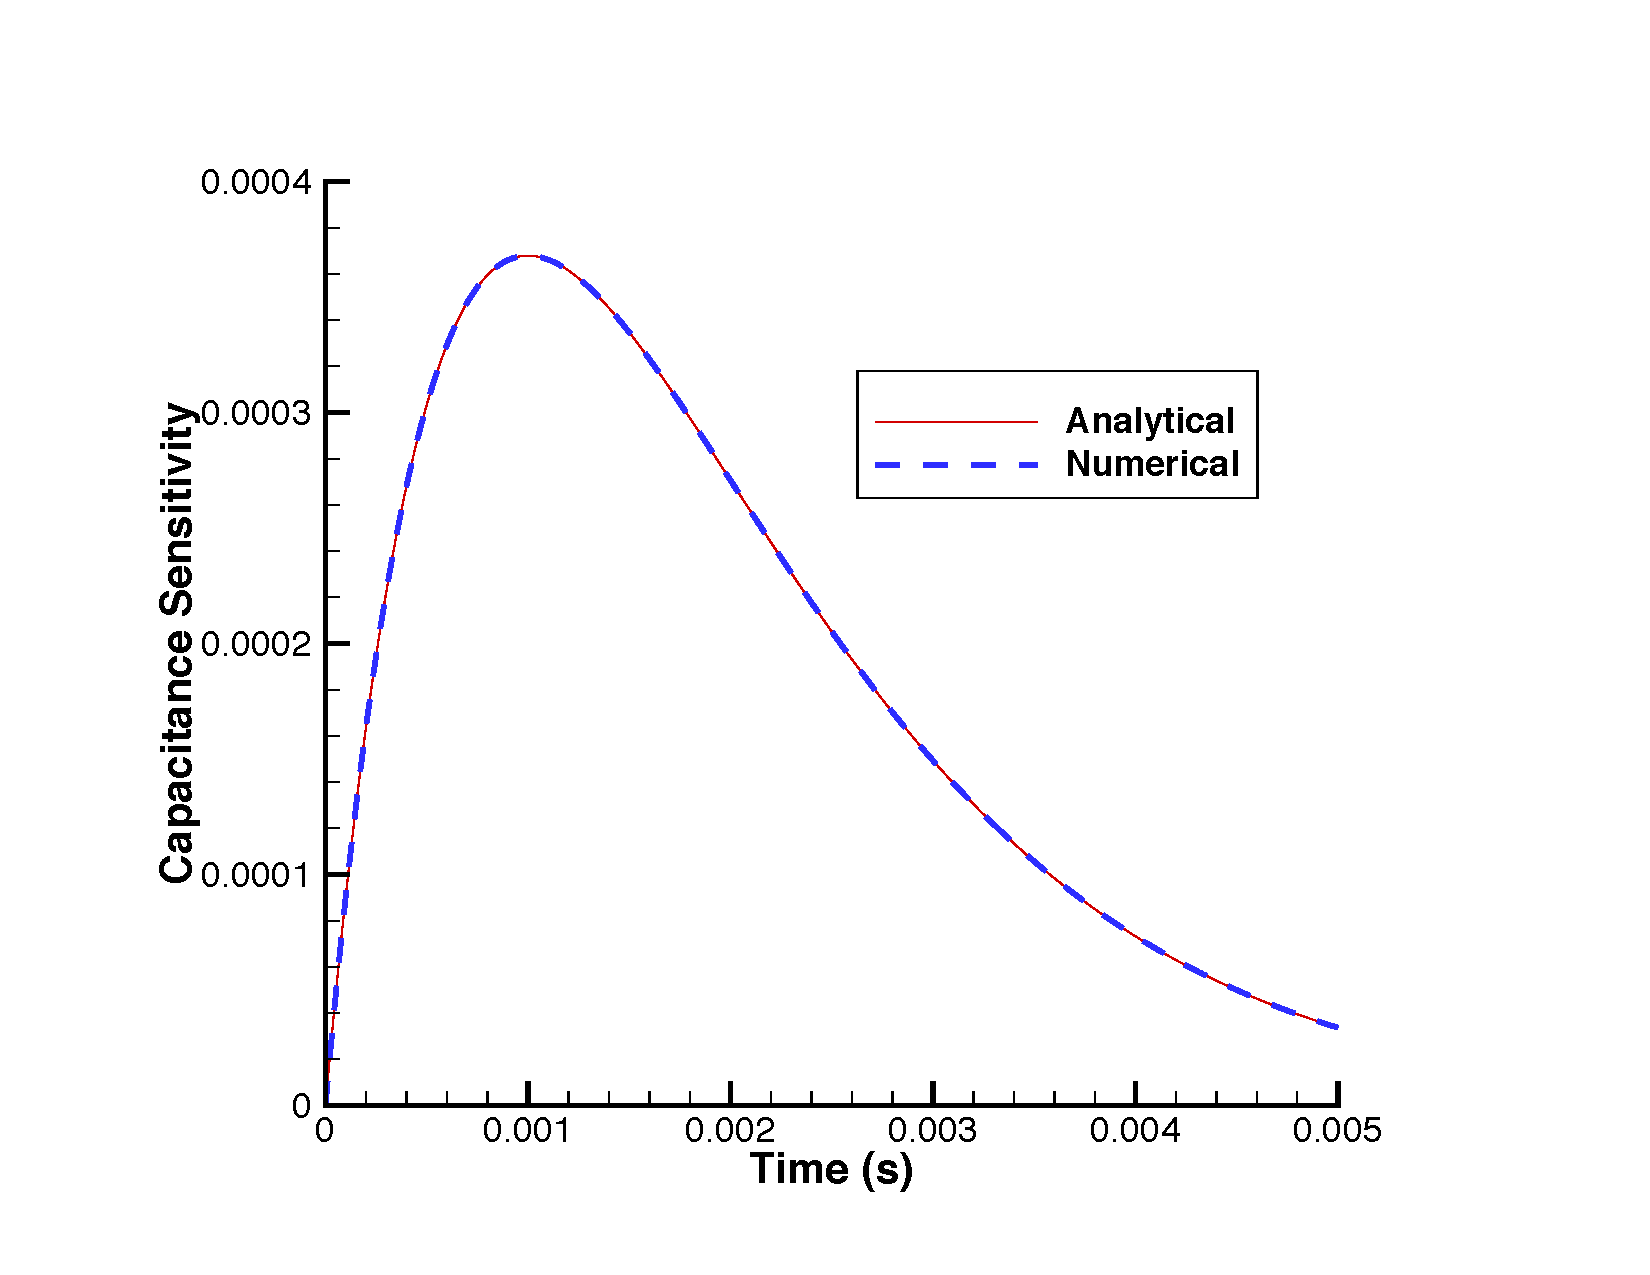
\includegraphics[]{sens}}
  \caption[Transient direct sensitivity result]
  {Transient direct sensitivity result.
\label{transientSensitivityResult}}
\end{figure}
Results for the transient example are given in figure~\ref{transientSensitivityResult}.
The analytic sensitivity solution is given by the solid line and the computed numerical
sensitivity is given by the dashed line.  The results match very well in this case,
with the two lines right on top of each other.

\clearpage
\subsubsection{Transient Adjoint Sensitivities}
Transient adjoint sensitivities are a good choice for really large
numbers of parameters, and when the number of objective functions is
modest.  For transient calculations, each time point is considered a
separate objective function, so it is best to use adjoints when the
sensitivity of interest concerns only one or a handful of time points.

Set \texttt{direct=0 adjoint=1} to specify transient adjoint
simulations.  The transient adjoint forumulation in \Xyce{} has
similarities to the ones described by Liu~\cite{Liu2014} and
Meir~\cite{BLAST2012}.  An example netlist for a transient adjoint
sensitivity calculation is given in
figure~\ref{Tran_Adjoint_Sensitivity_Netlist}.  This is a simple
linear problem (RC driven by a sinewave), so it has an analytic
solution.
\begin{figure}[htbp]
  \begin{centering}
    \shadowbox{
      \begin{minipage}{0.9\textwidth}
        \begin{vquote}
\color{blue}*Test of transient adjoint sensitivities \color{black}
.param cap=1e-6
.param res=1e3

V1 1 0 0.0 sin (0.0 1.0 200 0.0 0.0 0.0 )
R1 1 2 {res}
C1 2 0 {cap}

.tran 1.0e-6 0.5e-2
.print tran format=tecplot V(1) V(2) 
.print TRANADJOINT format=tecplot

.options timeint method=gear reltol=1.0e-6 abstol=1e-6

\color{red}* Sensitivity commands
.SENS objfunc={V(2)} param=R1:R,C1:C
.options SENSITIVITY direct=0 adjoint=1\color{black}
.end
\end{vquote}
\end{minipage}
}
\caption[Adjoint Transient Sensitivity Example Netlist]
{Adjoint Transient Sensitivity Example Netlist \label{Tran_Adjoint_Sensitivity_Netlist} }
\end{centering}
\end{figure}
\begin{figure}[ht]
  \centering
  \scalebox{0.5}
  {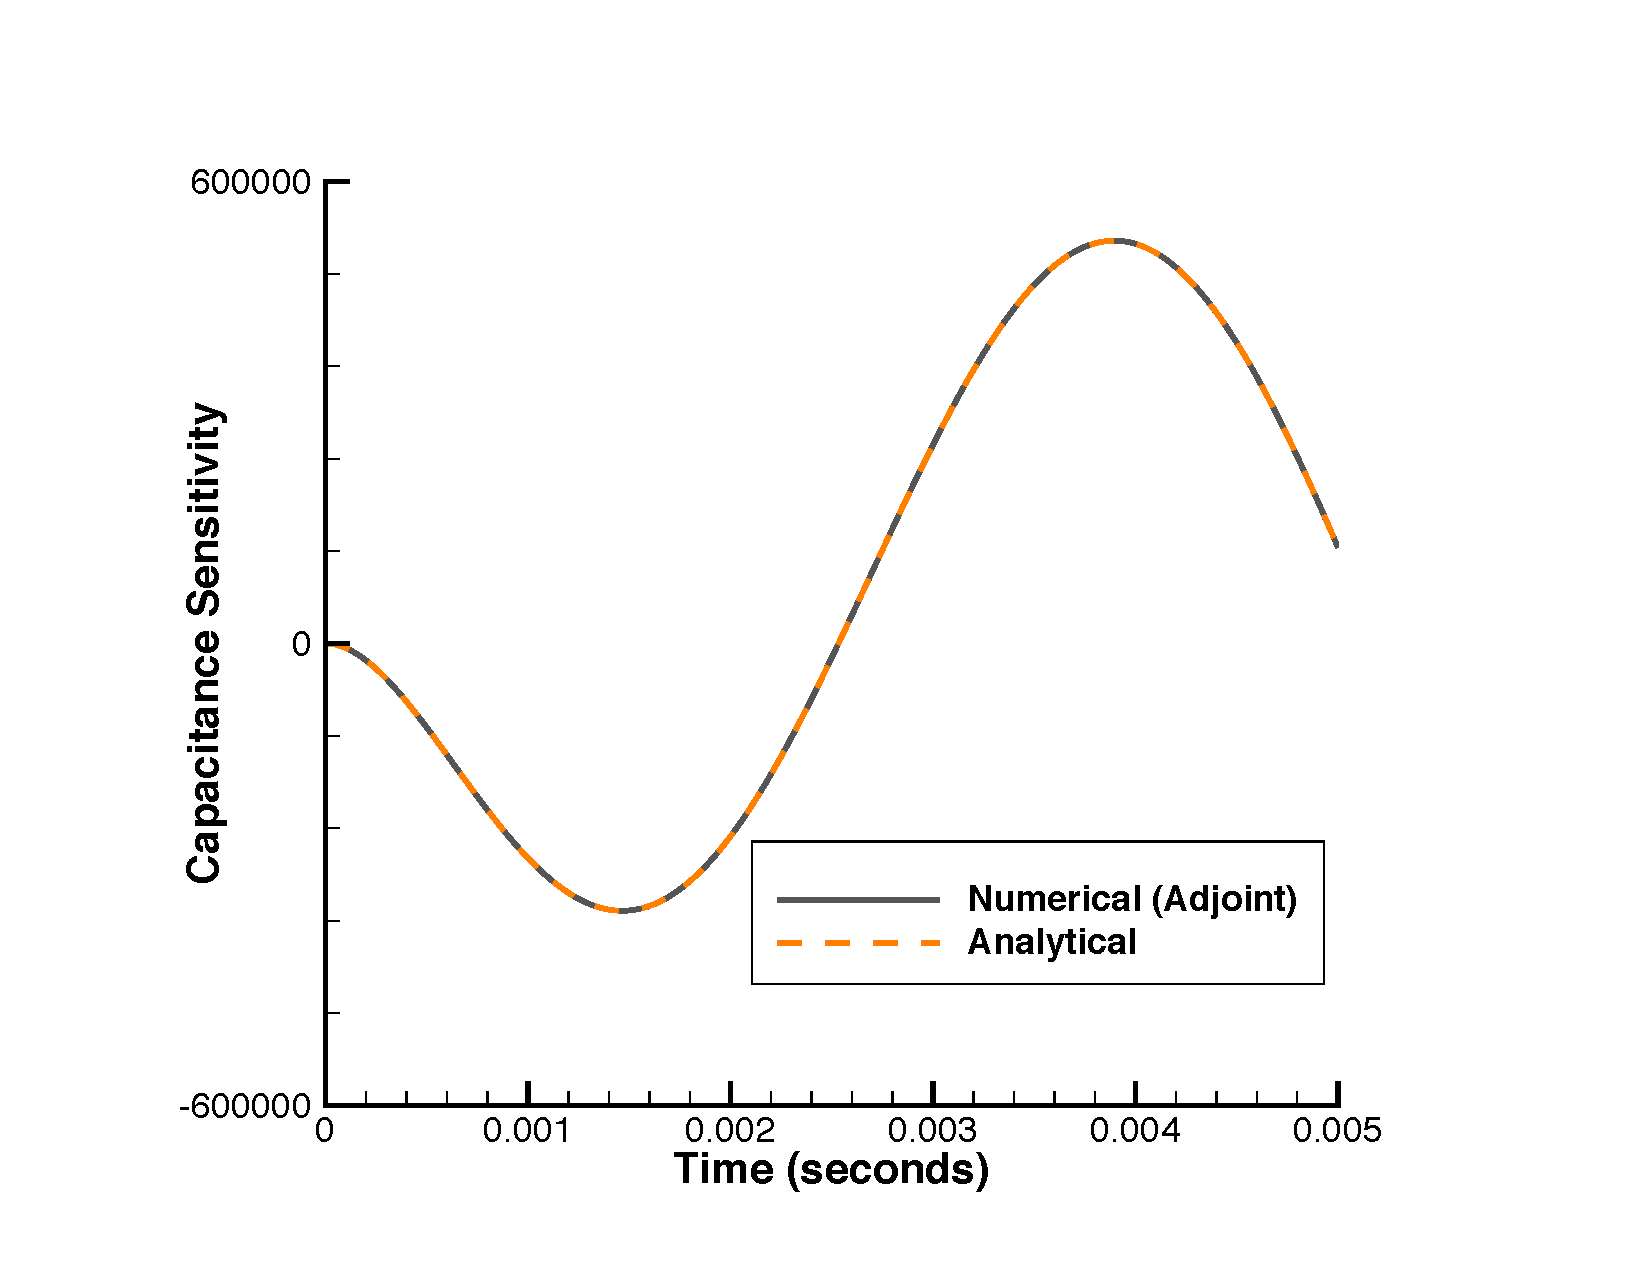
\includegraphics[]{sensCapGearAdj}}
  \caption[Transient adjoint sensitivity result]
  {Transient adjoint sensitivity result.
\label{transientAdjointSensitivityResult}}
\end{figure}
Results for the transient adjoint example are given in figure .  The
analytic sensitivity solution is given by the dashed line and the
computed numerical sensitivity is given by the solid line.  The
results match very well in this case, with the two lines right on top
of each other.

\clearpage
\subsection{AC Sensitivities}
Sensitivities can also be computed for small-signal AC analysis.  As
with steady-state (DC) and transient analysis, both direct and adjoint
sensitivities are supported.  An example netlist which exercises the
capability is shown in figure~\ref{AC_Sensitivity_Netlist}.

The netlist commands for AC sensitivities are very similar to those
for DC, but with some small exceptions.  The expression library in
\Xyce{} currently does not support complex numbers, so the
specification for objective functions is more limited.  As such, the
\texttt{objfunc} parameter will not work with AC sensitivities, and
the user should instead specify outputs using \texttt{objvars}
followed by a list of node names.  The sensitivities that are computed
will be for the voltages at the listed nodes, with respect to the list
of sensitivity parameters.
\begin{figure}[htbp]
  \begin{centering}
    \shadowbox{
      \begin{minipage}{0.99\textwidth}
        \begin{vquote}
\color{blue}*Lowpass filter test for AC sensitivities\color{black}
v1 1 0 ac 10.0
r1 1 2 4.7k
c1 2 0 47n

.ac dec 10 1 10k
.print ac  vm(1) vp(1) vm(2) vp(2)   
.print sens 

\color{red}* Sensitivity commands
.sens objvars=2 param=r1:r,c1:c
.options sensitivity direct=1 adjoint=0  stdoutput=1\color{black}
.end 
\end{vquote}
\end{minipage}
}
\caption[AC Sensitivity Example Netlist]
{AC Sensitivity Example Netlist \label{AC_Sensitivity_Netlist} }
\end{centering}
\end{figure}
For each specified output, there are four separate objective functions
for which sensitivities will be computed; magnitude and phase for the
polar representation, as well as real and imaginary for the cartesian
representation of the solution.  The console output for the example
netlist, for the first frequency, is shown in figure
~\ref{AC_Sensitivity_Result}.
\begin{figure}[htbp]
  \begin{centering}
    \shadowbox{
      \begin{minipage}{0.99\textwidth}
        \begin{vquote}

Direct Sensitivities for node V(2):
VR(2) = 1.0000e+01  VI(2) = -1.3880e-02
VM(2) = 1.0000e+01  VP(2) = -1.3880e-03

Name  Value Sensitivity\_Re  Sensitivity\_Im  Sensitivity\_Mag Sensitivity\_Phase
R1:R  4.7e+03  -8.1975e-09     -2.9531e-06     -4.0988e-09     -2.9531e-07
C1:C  4.7e-08  -8.1975e+02     -2.9531e+05     -4.0988e+02     -2.9531e+04

\end{vquote}
\end{minipage}
}
\caption[AC Sensitivity Example Result]
{AC Sensitivity Example Result\label{AC_Sensitivity_Result} }
\end{centering}
\end{figure}

\clearpage
\subsection{Output}
\label{SENS_Output}\index{\texttt{.PRINT}!\texttt{.SENS}}
For a full list and explanation of options related to \texttt{.SENS}
output see the \Xyce{} Reference Guide\ReferenceGuide{}.

Sensitivity output can be sent to standard output, or to a
user-specified log file.  The format for this output is similar to
that generated by the circuit given in
figure~\ref{DC_Sensitivity_Netlist}.  This feature is mainly made
available in \Xyce{} so as to be similar to the sensitivity analysis
of older circuit simulators.  However, for most uses it isn't the most
practical output, so it is disabled by default.  To enable standard
output, one should set the following:
\begin{verbatim}
.options SENSITIVITY STDOUTPUT=1
\end{verbatim}

In addition to the screen output, \Xyce{} can also produce a plottable
file containing all the requested sensitivities.  This file can be
requested by adding either a \texttt{.PRINT SENS} or a \texttt{.PRINT
  TRANADJOINT} command to the input file.  Steady-state sensitivities
(adjoint or direct) and transient direct sensitivities will be handled
by the \texttt{.PRINT SENS} command.  Transient adjoint, on the other
hand, is handled by the \texttt{.PRINT TRANADJOINT} command.

Unlike the traditional \texttt{.PRINT} line, both \texttt{.PRINT SENS}
and \texttt{.PRINT TRANADJOINT} will assume that the user wants all
the sensitivities specified on the \texttt{.SENS} line.  As such it is
not necessary (or possible) to specify specific sensitivities on the
\texttt{.PRINT SENS} line.  If the line exists, that is sufficient to
produce the file, and it will contain a column for every objective
function and every derivative.  The file name is the same as the one
produced with \texttt{.PRINT}, but with ``\texttt{.SENS}'' included
just before the suffix.  Similarly, for transient adjoint, the output
file name has the string ``\texttt{.TRADJ}'' included before the
suffix.  Note also, that most of the same output formats
(\texttt{std}, \texttt{tecplot}, etc.)  are available for
\texttt{.PRINT SENS} and\texttt{.PRINT TRANADJOINT} as they are for
conventional \texttt{.PRINT}.  The available formats are listed in
table~\ref{SENS_Output_table},~\ref{SENS_AC_Output_table}and~\ref{TRANADJOINT_Output_table}.
\begin{table}[htbp]
  \caption{Output generated for SENS analysis for .TRAN\label{SENS_Output_table}}
  \begin{tabularx}{\linewidth}{|p{2.75in}|Y|Y|}
    \rowcolor{XyceDarkBlue} \color{white}\textbf{Command} & \color{white}\textbf{Files} & \color{white}\textbf{Additional Columns} \\ \hline
\texttt{.PRINT SENS} & \emph{circuit-file}.SENS.prn & INDEX TIME \\ \hline
\texttt{.PRINT SENS FORMAT=GNUPLOT} & \emph{circuit-file}.SENS.prn & INDEX TIME \\ \hline
\texttt{.PRINT SENS FORMAT=SPLOT} & \emph{circuit-file}.SENS.prn & INDEX TIME \\ \hline
\texttt{.PRINT SENS FORMAT=NOINDEX} & \emph{circuit-file}.SENS.prn & INDEX TIME \\ \hline
\texttt{.PRINT SENS FORMAT=CSV} & \emph{circuit-file}.SENS.csv & TIME \\ \hline
\texttt{.PRINT SENS FORMAT=TECPLOT} & \emph{circuit-file}.SENS.dat & TIME \\ \hline
  \end{tabularx}
\end{table}
\begin{table}[htbp]
  \caption{Output generated for SENS analysis for .AC\label{SENS_AC_Output_table}}
  \begin{tabularx}{\linewidth}{|p{2.75in}|Y|Y|}
    \rowcolor{XyceDarkBlue} \color{white}\textbf{Command} & \color{white}\textbf{Files} & \color{white}\textbf{Additional Columns} \\ \hline
\texttt{.PRINT SENS} & \emph{circuit-file}.FD.SENS.prn & INDEX FREQ \\ \hline
\texttt{.PRINT SENS FORMAT=GNUPLOT} & \emph{circuit-file}.FD.SENS.prn & INDEX FREQ \\ \hline
\texttt{.PRINT SENS FORMAT=SPLOT} & \emph{circuit-file}.FD.SENS.prn & INDEX FREQ \\ \hline
\texttt{.PRINT SENS FORMAT=NOINDEX} & \emph{circuit-file}.FD.SENS.prn & INDEX FREQ \\ \hline
\texttt{.PRINT SENS FORMAT=CSV} & \emph{circuit-file}.FD.SENS.csv & FREQ \\ \hline
\texttt{.PRINT SENS FORMAT=TECPLOT} & \emph{circuit-file}.FD.SENS.dat & FREQ \\ \hline
  \end{tabularx}
\end{table}
As noted, transient adjoints are specified separately from
\texttt{.PRINT SENS}.  This is because the transient adjoint
calculation is performed as a post-process, after the original forward
calculation has been completed, and \Xyce{}'s forward outputters are
no longer active.  To specify transient adjoint output, one must use
\texttt{.PRINT TRANADJOINT} instead.  As it is possible to perform
both a transient direct and a transient adjoint calculation as part of
the same computation, and most of \Xyce{}'s output files are in column
format, there wasn't an easy way to have them use the same outputter.
\begin{table}[htbp]
  \caption{Output generated for transient adjoint SENS analysis \label{TRANADJOINT_Output_table}}
  \begin{tabularx}{\linewidth}{|p{2.75in}|Y|Y|}
    \rowcolor{XyceDarkBlue} \color{white}\textbf{Command} & \color{white}\textbf{Files} & \color{white}\textbf{Additional Columns} \\ \hline
\texttt{.PRINT TRANADJOINT} & \emph{circuit-file}.TRADJ.prn & INDEX TIME \\ \hline
\texttt{.PRINT TRANADJOINT FORMAT=NOINDEX} & \emph{circuit-file}.TRADJ.prn & INDEX TIME \\ \hline
\texttt{.PRINT TRANADJOINT FORMAT=CSV} & \emph{circuit-file}.TRADJ.csv & TIME \\ \hline
\texttt{.PRINT TRANADJOINT FORMAT=TECPLOT} & \emph{circuit-file}.TRADJ.dat & TIME \\ \hline
  \end{tabularx}
\end{table}

\clearpage
\subsection{Notes about .SENS accuracy and formulation}
The sensitivity calculation in \Xyce{} is based on a chain rule
calculation.  Ultimately, the calculation will produce $dO/dp$, where
$O$ is a user-specified objective function, and $p$ is a
user-specified parameter.  $dO/dp$ is equal to:
\begin{equation}
  \frac{dO}{dp} = \frac{\partial O}{\partial x}\frac{\partial x}{\partial p} + \frac{\partial O}{\partial p}
  \label{objectiveDerivative}
\end{equation}
\noindent where $x$ is a solution vector and $\partial x/\partial p$
is the sensitivity of that solution vector with respect to the
parameter.  Evaluating~\ref{objectiveDerivative} requires that
$\partial x/\partial p$ be computed first.  The direct sensivity
calculation for $\partial x/\partial p$ can be derived by considering
the DAE form of the residual equation:
\begin{equation}
  F(x,t) = \dot{q}(x,t) + j(x,t) - b(t) = 0
  \label{residual}
\end{equation}
\noindent In this equation, $q$ represents quantities that must be
differentiated with respect to time (such as capacitor charge), and
$j$ represents algebraic terms that depend on the solution $x$ (such
as DC currents), and $b$ are independent sources that only depend on
time.  Equation~\ref{residual} is solved to obtain the solution, $x$.
To obtain sensitivities, one must differentiate this equation with
respect to a parameter, $p$.
\begin{equation}
  \frac{dF}{dp} = \frac{d}{dp}\left( \dot{q} + j - b \right) = 0
  \label{dfdp}
\end{equation}
In steady-state, equation~\ref{dfdp} simplifies to:
\begin{equation}
  \frac{dF}{dp} = \frac{dj}{dp} - \frac{db}{dp} = 0
  \label{steady_dfdp}
\end{equation}
\noindent As $j$ is dependent upon $x$, the $\frac{dj}{dp}$ term must
be expanded via chain rule, and the resulting equation must be
re-arranged to set up a matrix equation that can be solved to obtain
$\frac{dx}{dp}$:
\begin{equation}
  \frac{dj}{dx}\frac{dx}{dp} = - \frac{dj}{dp} + \frac{db}{dp} 
  \label{finalSens}
\end{equation}
\noindent In equation~\ref{finalSens}, the terms on the right hand
side are computed by the individual device models once the Newton loop
the circuit analysis has converged.  The Jacobian matrix on the left
hand side ($dj/dx$) is the same matrix used by the original analysis.
Once the linear system is solved, then $dx/dp$ is available for the
given parameter, and it can then be applied to
equation~\ref{objectiveDerivative}.  For transient, a similar linear
system is solved, which depends on the specific time integration
method used.  For Backward-Euler the linear system is:
\begin{equation}
  \left[ \frac{1}{h} \frac{dq}{dx} 
  + \frac{dj}{dx} \right] \frac{dx}{dp}_{n+1} 
 =
  -\frac{1}{h} \left[ \frac{dq}{dp}_{n+1} - \frac{dq}{dp}_n \right] 
 - \frac{dj}{dp} 
 + \frac{db}{dp} 
 + \frac{1}{h} \left[ \frac{dq}{dx} \right] \frac{dx}{dp}_n 
 \label{finalTransientSens}
\end{equation}
\noindent Where $h$ is the time step size.  As with ~\ref{finalSens},
the left hand side of the equation contains the original Jacobian
matrix.

In general, the accuracy of the above calculation is dependent on the
accuracy of the individual derivatives that comprise
equations~\ref{objectiveDerivative} and~\ref{finalSens}
or~\ref{finalTransientSens}.  In \Xyce{}, the Jacobian derivatives
($dj/dx$ and $dq/dx$) are always analytic.  Similarly, the objective
function derivatives ($dO/dx$) are also always analytic.  However, the
derivatives on the right hand side of~\ref{finalTransientSens}
($dj/dp$, $db/dp$ and $dq/dp$) depend on particular device
implementations.  If the device was implemented with analytic
parameter sensitivies, then those sensitivities are used.  If analytic
derivatives were not available, then the $dj/dp$, $dq/dp$ and $db/dp$
derivatives are computed using finite differences.  A list of \Xyce{}
devices, and which of them support analytic sensitivities, is given in
the \Xyce{} Reference Guide\ReferenceGuide{}.

For some problems, finite difference derivatives will work fine, but
some devices and/or circuit problems have wide ranges of solution
and/or parameter scalings, and this can render inaccurate finite
difference derivatives.  As this capability develops, most devices
should eventually provide analytic derivatives.

The above derivation and arguments were given for direct sensitivities
(as that is the only form supported for both DC and transient), but
the same ideas with regard to accuracy apply for adjoint sensitivites.

For transient, note that the transient direct calculation uses the
same time steps that are used for the original circuit analysis.  It
does not impose any additional error control that is specific to the
accuracy of $dx/dp$.

%%%%%%
% -------------------------------------------------------------------------
% S-parameter (.LIN) Analysis Section -------------------------------------
% -------------------------------------------------------------------------

\section{S-parameter Analysis}
\label{SP_Analysis}
\label{SP_Sweep_Overview}
\index{analysis!S-parameter} \index{S-parameter analysis} \index{\texttt{.LIN}}
\index{AC sweep} \index{analysis!AC sweep}

The S-parameter small-signal analysis of \Xyce{} computes linear
transfer parameters as a function of frequency for a general
multi-port network. The program first computes the DC operating point
of the circuit and then linearizes the circuit. The resultant linear
circuit is then analyzed over a user-specified range of
frequencies. The output of a S-parameter analysis is multi-port
scattering (S) parameters. The S-parameters represent the ratio of
incident and scattered normalized voltage waves.  The analysis results
can also be output as Y-parameter or Z-parameter values.

\subsection{.LIN Statement}

One may specify S-parameter analyses by using a \verb|.LIN| command with a \verb|.AC| command in the netlist.
Here is an example of typical \verb|.AC| and \verb|.LIN| lines:

\Example{\\
\texttt{.AC DEC 10 1K 100MEG}  \\
\texttt{.LIN sparcalc=1 format=touchstone}  \\
}

The \verb|.LIN| analysis is similar to a basic small signal \verb|.AC|
analysis, but it also calculates small signal transfer parameters
between terminals identified using port (P) devices. The \Xyce{}
Reference Guide\ReferenceGuide{} provides a complete description of
\verb|.LIN| analysis and the P device.  To output Y-parameter or
Z-parameter values instead the \texttt{LINTYPE=Y} or
\texttt{LINTYPE=Z} argument can be used on the \texttt{.LIN} line.

\subsection{Port Devices}
\label{SP_Port}
\index{S-parameter analysis!port}

The \verb|.LIN| analysis computes the S-parameters based on the
location of the port (P) devices and the values of their reference
impedances. The port devices identify the ports used in \verb|.LIN|
analysis. The \Xyce{} Reference Guide\ReferenceGuide{} provides a
complete description of the port devices. Some examples are as
follows:

\Example{\\   
%\texttt{*name nodelist type value  phase(deg)}  \\
\texttt{P1 1 0 port = 1} \\
\texttt{P2 12 0  port= 2  z0=100 }
}

NOTE: Each port requires a unique port number. If a circuit has N
ports, the netlist must contain the sequential set of port numbers, 1
to N.

\subsection{Example}
An example S-parameter analysis netlist is given in
figure~\ref{spExample}.  This example uses 2 ports.  The S parameters
are output to a file in Touchstone 1 format
\cite{touchstone2_std_2009}.  Touchstone 2 format is also supported.
Note that \texttt{SPARCALC=1} is specified on the \texttt{.LIN} line.
If \texttt{SPARCALC=0} is specified instead then a \texttt{.AC}
analysis will be done.

\begin{figure}[htbp]
  \begin{centering}
    \shadowbox{
      \begin{minipage}{0.9\textwidth}
        \begin{vquote}
\color{blue}* S-parameter Analysis example\color{black}
P1 1 0 port= 1
~
C1 2 0 1e-2
Rgs 1 2 0.02

.subckt RCBlock IN OUT GND
R1 IN OUT 20
C1 IN OUT 1p
Cg1 OUT GND 1p
.ends

X1 2 3 0 RCBlock
X2 3 4 0 RCBlock
X3 4 5 0 RCBlock
X4 5 6 0 RCBlock
X5 6 7 0 RCBlock
X6 7 8 0 RCBlock
X7 8 9 0 RCBlock
X8 9 10 0 RCBlock
X9 10 11 0 RCBlock
X10 11 12 0 RCBlock

.AC DEC 10 10  1e5 

.LIN FORMAT=TOUCHSTONE  sparcalc=1

P2 12 0  port=2 z0=100

.END

\end{vquote}
\end{minipage}
}
\caption[S-parameter Example Netlist]
{S-parameter Example Netlist.  \label{spExample} }
\end{centering}
\end{figure}

\subsection{Output}
\label{LIN_Output}
For S-parameter analysis, the output is controlled by the \texttt{.LIN}
command when \texttt{SPARCALC=1} on that line.  Any information on
\texttt{.PRINT AC} lines will be ignored in that case.
Table~\ref{LIN_Output_table} lists the format options and files created.
If \texttt{SPARCALC=0} then a \texttt{.AC} analysis is done instead.

All three data formats defined in the Touchstone standard, which are
real-imaginary (RI), magnitude-angle(MA) and magnitude(db)-angle (DB),
are supported.  The default is RI.  Other options can be selected via
the inclusion of the \texttt{DATAFORMAT=<val>} argument on the
\texttt{.LIN} line. Per the Touchstone standard, all angle values are
output in degrees.

The default filename for both Touchstone formats is
\texttt{<netlistName>.sNp} where N is the number of ``ports''
(\texttt{P} devices) specified in the netlist.  The output can be
redirected to another file with the \texttt{-o} command line option or
by using a \texttt{FILE=<filename>} argument on the \texttt{.LIN}
line.

The default output is S-parameters.  The \texttt{LINTYPE=<S|Y|Z>}
argument can be used on the \texttt{.LIN} line to select Y-parameter
or Z-parameter output instead.  (Note: The default filename is still
\texttt{<netlistName>.sNp} even if the output file contains
Y-parameter or Z-parameter output rather than S-parameter output.)
The \Xyce{} Reference Guide\ReferenceGuide{} has a complete listing of
which arguments, typically used on a \texttt{.PRINT} line also work on
a \texttt{.LIN} line.

\begin{table}[htbp]
  \caption{Output generated for .LIN analysis \label{LIN_Output_table}}
  \begin{tabularx}{\linewidth}{|p{2.75in}|Y|Y|}
    \rowcolor{XyceDarkBlue} \color{white}\textbf{Command} & \color{white}\textbf{Files} & \color{white}\textbf{Format} \\ \hline
\texttt{.LIN} & \emph{circuit-file}.sNp & S-parameter data in Touchstone 2 format. Data format is RI. \\ \hline
\texttt{.LIN FORMAT=TOUCHSTONE} & \emph{circuit-file}.sNp & S-parameter data in Touchstone 1 format. Data format is RI. \\ \hline
\texttt{.LIN FORMAT=TOUCHSTONE2} & \emph{circuit-file}.sNp & S-parameter data in Touchstone 2 format. Data format is RI. \\ \hline
\texttt{.LIN DATAFORMAT=MA} & \emph{circuit-file}.sNp & S-parameter data in Touchstone 2 format. Data format is MA. \\ \hline
\texttt{.LIN DATAFORMAT=DB} & \emph{circuit-file}.sNp & S-parameter data in Touchstone 2 format. Data format is DB. \\ \hline
\texttt{.LIN LINTYPE=Y} & \emph{circuit-file}.sNp & Y-parameter data in Touchstone 2 format. Data format is RI. \\ \hline
\texttt{.LIN LINTYPE=Z} & \emph{circuit-file}.sNp & Z-parameter data in Touchstone 2 format. Data format is RI. \\ \hline

\texttt{\emph{Xyce} -r} & NA & This will produce a parsing error. \\ \hline
\texttt{\emph{Xyce} -r -a} & NA & This will produce a parsing error. \\ \hline

\end{tabularx}
\end{table}

When a \texttt{.LIN} analysis is done then additional output variable
formats are available via the \texttt{.PRINT AC} line, where
\texttt{<index1>} and \texttt{<index2>} must both be greater than 0
and also both less than or equal to the number of ports in the
netlist:
\begin{XyceItemize}
\item \texttt{SR(<index1>,<index2>)} to output the real component of an S-parameter
\item \texttt{SI(<index1>,<index2>)} to output the imaginary component of an S-parameter
\item \texttt{SM(<index1>,<index2>)} to output the magnitude of an S-parameter
\item \texttt{SP(<index1>,<index2>)} to output the phase of an S-parameter in degrees
\item \texttt{SDB(<index1>,<index2>)} to output the magnitude of an S-parameter in decibels.
\item \texttt{YR(<index1>,<index2>)} to output the real component of a Y-parameter
\item \texttt{YI(<index1>,<index2>)} to output the imaginary component of a Y-parameter
\item \texttt{YM(<index1>,<index2>)} to output the magnitude of a Y-parameter
\item \texttt{YP(<index1>,<index2>)} to output the phase of a Y-parameter in degrees
\item \texttt{YDB(<index1>,<index2>)} to output the magnitude of a Y-parameter in decibels.
\item \texttt{ZR(<index1>,<index2>)} to output the real component of a Z-parameter
\item \texttt{ZI(<index1>,<index2>)} to output the imaginary component of a Z-parameter
\item \texttt{ZM(<index1>,<index2>)} to output the magnitude of a Z-parameter
\item \texttt{ZP(<index1>,<index2>)} to output the phase of a Z-parameter in degrees
\item \texttt{ZDB(<index1>,<index2>)} to output the magnitude of a Z-parameter in decibels.
\end{XyceItemize}

\Example{\\
\texttt{.print AC SR(1,1) YI(1,2) ZM(2,1)}
}

%%% Local Variables:
%%% mode: latex
%%% End:
% END of Xyce_UG_ch09.tex ************

\cleardoublepage
% Sandia National Laboratories is a multimission laboratory managed and
% operated by National Technology & Engineering Solutions of Sandia, LLC, a
% wholly owned subsidiary of Honeywell International Inc., for the U.S.
% Department of Energy’s National Nuclear Security Administration under
% contract DE-NA0003525.

% Copyright 2002-2022 National Technology & Engineering Solutions of Sandia,
% LLC (NTESS).

%%-------------------------------------------------------------------------
%% Purpose        : Main LaTeX Xyce Users' Guide
%% Special Notes  : Graphic files (pdf format) work with pdflatex.  To use
%%                  LaTeX, we need to use postcript versions.  Not sure why.
%% Creator        : Scott A. Hutchinson, Computational Sciences, SNL
%% Creation Date  : {05/23/2002}
%%
%%-------------------------------------------------------------------------

% -------------------------------------------------------------------------
% Homotopy/Continuation Analysis Chapter ----------------------------------
% -------------------------------------------------------------------------

\chapter{Homotopy and Continuation Methods}
\label{Homotopy_Chap}
\index{homotopy}

\index{continuation}
\index{continuation}
%\index{bifurcation}

\chapteroverview{Chapter Overview}
{
This chapter includes the following sections:
\begin{XyceItemize}
\item Section~\ref{continuation_Overview}, {\em Continuation Algorithms Overview}
\item Section~\ref{continuation_natural},  {\em Natural Parameter Continuation}
\item Section~\ref{continuation_natural_multiparam}, {\em Natural Multiparameter Continuation}

\item Section~\ref{continuation_gmin},    {\em GMIN Stepping Continuation}
\item Section~\ref{continuation_source},    {\em Source Stepping Continuation}
\item Section~\ref{continuation_mosfet},   {\em MOSFET Continuation}

\item Section~\ref{continuation_pseudotran}, {\em Pseudo Transient}
\item Section~\ref{continuation_arclength}, {\em Arc Length Continuation}
\end{XyceItemize}
}

%%%%%%%%%%%%%%%%%%%%%%%%%%%%%%%%%%%%%%%%%%%%%%%%%%%%%%%%%%%%%%%%%%%%%%%%%%%%%%%%
\section{Continuation Algorithms Overview}

\label{continuation_Overview}
\index{continuation}

Often, circuit convergence problems are most prominent during the DC operating
point calculation. Unlike transient solves, DC operating point analysis cannot
rely on a good initial guess from a previous step, and cannot simply reduce the
step size when the solver fails. Additionally, operating points often have
multiple solutions, with no capability to interpret the user's intent. Multiple
solutions can, even for converged circuit problems, result in a standard Newton
solve being unreliable. For example, the operating point solution to a Schmidt
trigger circuit has been observed to change with the computational platform.

Continuation methods can often provide solutions to difficult nonlinear problems,
including circuit analysis, even when conventional methods (e.g., Newton's
method) fail ~\cite{Melville:1990} ~\cite{Melville:1993}.  This chapter gives
an introduction to using continuation algorithms (sometimes called homotopy 
algorithms) in \Xyce{}. The \Xyce{} Reference Guide\ReferenceGuide{} provides a
more complete description of solver options.

The underlying numerical library used by \Xyce{} to support continuation methods
is LOCA (Library of Continuation Algorithms)~\cite{loca,loca2}.  For a description 
of the numerical details see the LOCA theory and implementation 
manual~\cite{locaManual}.

\subsection{Continuation Algorithms Available in \Xyce{}}

\Xyce{} invokes a well-known SPICE method, ``GMIN stepping,'' automatically
when a DC operating point fails to converge without it.  It is a special case
where the parameter being swept is artificial.  GMIN stepping can also be
invoked with \texttt{.options nonlin continuation=3} or \texttt{.options nonlin
continuation=gmin}. See Section~\ref{continuation_gmin} for more information and an
example of GMIN stepping.

\Xyce{} also invokes the SPICE ``source stepping'' method automatically when a DC operating point calculation fails both normal Newton's method and the automatic GMIN stepping attempt.  This is an example of natural parameter continuation that steps through a scale factor that is applied to all DC voltage sources in the circuit.  It is described in Section~\ref{continuation_source}.

Another basic type of continuation in \Xyce{} is accessed by setting
\texttt{.options nonlin continuation=1}. This allows the user to sweep existing
device parameters (models and instances), as well as a few reserved artificial
parameter cases. The most obvious natural parameter to use is the magnitude(s)
of independent voltage or current sources, the choice of which is equivalent to
``source stepping'' in SPICE.  Section~\ref{continuation_natural} provides a
\Xyce{} source-stepping example.  For some circuits (as in the aforementioned
Schmidt trigger), source stepping leads to turning points in the continuation.  

A special type of continuation, an algorithm designed specifically for MOSFET
circuits~\cite{ROYCHOWDHURY:2003}, involves two internal MOSFET model
parameters---one for the MOSFET gain, and the other for the nonlinearity of the
current-voltage relationship.  This algorithm is invoked with \texttt{.options
nonlin continuation=2}, and has proven to be effective in some large MOSFET
circuits.  Section~\ref{continuation_mosfet} provides a detailed example.

%%%%%%%%%%%%%%%%%%%%%%%%%%%%%%%%%%%%%%%%%%%%%%%%%%%%%%%%%%%%%%%%%%%%%%%%%%%%%%%%
\newpage 
\section{Natural Parameter Continuation}
\label{continuation_natural}
\index{continuation!natural}
\index{continuation!natural}

Figure~\ref{Continuation_Netlist_sourceStepping} shows a natural parameter
continuation netlist with parameters pertinent to the continuation algorithm
highlighted in red.  For this example, the parameter being swept is
the DC value of the voltage source \texttt{VDDdev}.  This
example demonstrates a version of ``source stepping'' that is similar to SPICE,
but only applied to the single voltage source \texttt{VDDdev} rather than to all 
voltage sources.  For an example of source stepping in which every source 
in simultaneously swept, see sections~\ref{continuation_scaling} and~\ref{continuation_source}.

Using continuation on the magnitudes of independent voltage and current sources 
is a fairly obvious technique when a DC operating point calculation fails to 
converge.  However, a na\"{\i}ve application of natural parameter continuation
to single voltage and current sources does not often enable convergence in practice.  
Xyce will apply source stepping automatically during the DC operating point calculation 
if both the standard Newton's method and GMIN stepping fail.  So, normally, this 
technique of manually forcing stepping of a single source is unnecessary.

\begin{figure}[htbp]
\begin{centering}
\shadowbox{
\begin{minipage}{0.8\textwidth}
\begin{vquote}
\color{blue}MOS level 1 model CMOS inverter\color{black}
.TRAN 20ns 30us 0 5ns
.PRINT tran v(vout) v(in) v(1)
.options timeint reltol=5e-3 abstol=1e-3 \color{XyceRed}
* Continuation Options

.options nonlin continuation=1
.options loca stepper=0 predictor=0 stepcontrol=1
+ conparam=VDDdev
+ initialvalue=0.0 minvalue=-1.0 maxvalue=5.0
+ initialstepsize=0.2 minstepsize=1.0e-4 
+ maxstepsize=5.0 aggressiveness=1.0
+ maxsteps=100 maxnliters=200
\color{black}
VDDdev 	VDD	0	5V
RIN	IN	1	1K
VIN1  1	0  5V PULSE (5V 0V 1.5us 5ns 5ns 1.5us 3us)
R1    VOUT  0  10K  
C2    VOUT  0  0.1p 
MN1   VOUT  IN 0   0   CD4012_NMOS  L=5u W=175u         
MP1   VOUT  IN VDD VDD CD4012_PMOS  L=5u W=270u         
.MODEL cd4012_pmos PMOS 
.MODEL cd4012_nmos NMOS 
.END
\end{vquote}
\end{minipage}
}
\caption[Example natural parameter continuation netlist]{Example natural parameter continuation netlist. This example of source stepping shows a circuit that does not require continuation to run. Most circuits complex enough to require continuation would not fit on a single page.\label{Continuation_Netlist_sourceStepping}}
\end{centering}
\end{figure}

\subsection{Explanation of Parameters, Best Practice}
\label{locaParameterExplanation}

Figure~\ref{Continuation_Netlist_sourceStepping} also illustrates the following ``best practice'' rules:

\begin{XyceItemize}
\item \texttt{.options nonlin continuation=1}.  Sets the algorithm to use natural
parameter continuation.
\item \texttt{.options loca conparam=VDDdev}.  If using natural parameter continuation, it is necessary include a setting for \texttt{conparam}.  It sets which input parameter to use to perform continuation.  The parameter name is subject to the same rules as parameter used by the \texttt{.STEP} capability. (Section~\ref{step_InstanceParam}).  In this case, the parameter is the
magnitude of the DC voltage source, VDDdev.  For this type of voltage
source, it was possible to use the default device parameter (Section~\ref{step_SpecialCases})
\item \texttt{.options loca initialvalue=0.0}.  This is required.
\item \texttt{.options loca maxvalue=5.0}.  This is required.
\item \texttt{.options loca stepcontrol=1} or \texttt{.options loca stepcontrol=adaptive}.  This specifies the continuation steps to be adaptive, rather than constant.  This is recommended.
\item \texttt{.options loca maxsteps=100}.  This sets the maximum number of continuation 
steps for each parameter.  
\item \texttt{.options loca maxnliters=200}.  This is the maximum number of nonlinear 
iterations, and has precedence over the similar number that can be set on
the \texttt{.options nonlin} line.
\item \texttt{.options loca aggressiveness=1.0}.  This refers to the step size 
control algorithm,
and the value of this parameter can be anything from 0.0 to 1.0.  1.0 is
the most aggressive.  In practice, try starting with this set to 1.0. 
If the solver fails, then reset to a smaller number.
\end{XyceItemize}

\subsection{Voltage Source Scaling Continuation}
\label{continuation_scaling}
\index{continuation!natural!Voltage Source Scaling}
\index{continuation!natural!Voltage Source Scalaing}

Figure~\ref{Continuation_Netlist_sourceStepping2} shows a natural
parameter continuation netlist with parameters pertinent to the
continuation algorithm highlighted in red.  For this example, a
special parameter \texttt{VSRCSCALE} is being swept from zero to one.
This parameter is applied as a scaling factor for all DC voltage
sources in the netlist.  As a result, this example demonstrates an
explicit invocation of ``source stepping'' like the one that both
\Xyce{} and SPICE apply automatically as part of their DC operating
point solution strategies if Newton's method and GMIN stepping both
fail.

\begin{figure}[htbp]
\begin{centering}
\shadowbox{
\begin{minipage}{0.8\textwidth}
\begin{vquote}
\color{blue}*Simple netlist demonstrating source-stepping continuation
*This source will be swept with .DC \color{black}
V1 1 0 DC 1
R1 1 0 100
\color{blue}*This source will be not swept with .DC \color{black}
V2 2 0 DC 8
R2 2 0 100
.DC V1 1 8 1
.print DC V(1) V(2)
.print HOMOTOPY V(1) V(2)
* Continuation Options
.options nonlin continuation=1

.options loca stepper=0 predictor=0 stepcontrol=0
+ conparam=vsrcscale
+ initialvalue=0.0 minvalue=-1.0 maxvalue=1.0
+ initialstepsize=0.2 minstepsize=1.0e-4 maxstepsize=0.2
+ aggressiveness=1.0
+ maxsteps=5000 maxnliters=200
\color{black}
.END
\end{vquote}
\end{minipage}
}
\caption[Example natural parameter continuation netlist]{Example natural parameter continuation netlist implementing source stepping over all DC voltage sources. This example of source stepping shows a circuit that does not require continuation to run. Most circuits complex enough to require source stepping would not fit on a single page.\label{Continuation_Netlist_sourceStepping2}}
\end{centering}
\end{figure}

%%%%%%%%%%%%%%%%%%%%%%%%%%%%%%%%%%%%%%%%%%%%%%%%%%%%%%%%%%%%%%%%%%%%%%%%%%%%%%%%
\newpage 
\section{Natural Multiparameter Continuation} 
%Per The Chicago Manual of Style, 7.85, ``Compunds formed with prefixes are normally closed, whether %they are nouns, verbs, adjectives, or adverbs.'' There are exceptions, but multiparameter is not one. TT
\label{continuation_natural_multiparam}

It is possible to use the natural parameter continuation specification to  
have \Xyce{} sweep multiple parameters in sequential order.  This 
requires specifying many of the parameters in the \texttt{.options loca} statement as vectors, delineated by commas, rather than as single parameters.  

%An example, which manually reproduces the MOSFET
%continuation example from figure~\ref{Continuation_Netlist_1}, is given in 
%figure~\ref{Continuation_Netlist_multiParam}.

This is a usage example --- the circuit itself does not require continuation to run. Most circuits complex enough to require continuation would not fit on a single page.  

\subsection{Explanation of Parameters, Best Practice}

The solver parameters set in figure~\ref{Continuation_Netlist_multiParam} are 
the same as those from figure~\ref{Continuation_Netlist_sourceStepping}, but many of them
are in vector form.  Specify any parameters specific to the 
continuation variable as a vector, including \texttt{conparam}, \texttt{initialvalue},
 \texttt{minvalue}, \texttt{maxvalue}, \texttt{initialstepsize},
 \texttt{minstepsize}, \texttt{maxstepsize}, and \texttt{aggressiveness}.
Otherwise, the specification is identical.

\begin{figure}[htbp]
\begin{centering}
\shadowbox{
\begin{minipage}{0.8\textwidth}
\begin{vquote}
\color{blue}MOS level 1 model CMOS inverter\color{black}
.TRAN 20ns 30us 0 5ns
.PRINT tran v(vout) v(in) v(1)
.options timeint reltol=5e-3 abstol=1e-3 \color{XyceRed}
* Continuation Options
.options nonlin continuation=1
.options loca stepper=0 predictor=0 stepcontrol=adaptive
+ conparam=mosfet:gainscale,mosfet:nltermscale
+ initialvalue=0.0,0.0 
+ minvalue=-1.0,-1.0 
+ maxvalue=1.0,1.0
+ initialstepsize=0.2,0.2 
+ minstepsize=1.0e-4,1.0e-4 
+ maxstepsize=5.0,5.0 
+ aggressiveness=1.0,1.0
\color{black}
VDDdev 	VDD	0	5V
RIN	IN	1	1K
VIN1  1	0  5V PULSE (5V 0V 1.5us 5ns 5ns 1.5us 3us)
R1    VOUT  0  10K  
C2    VOUT  0  0.1p 
MN1   VOUT  IN 0   0   CD4012_NMOS  L=5u W=175u         
MP1   VOUT  IN VDD VDD CD4012_PMOS  L=5u W=270u         
.MODEL cd4012_pmos PMOS 
.MODEL cd4012_nmos NMOS 
.END
\end{vquote}
\end{minipage}
}
\caption [Example multiparameter continuation netlist]{Example multiparameter continuation netlist. 
This netlist reproduces MOSFET continuation with a manual specification. \label{Continuation_Netlist_multiParam}}


\end{centering}
\end{figure}



%%%%%%%%%%%%%%%%%%%%%%%%%%%%%%%%%%%%%%%%%%%%%%%%%%%%%%%%%%%%%%%%%%%%%%%%%%%%%%%%
\newpage 
\section{GMIN Stepping}
\label{continuation_gmin}
\index{continuation!GMIN Stepping}

GMIN stepping is a type of continuation commonly available in circuit simulators.
Like SPICE, \Xyce{} automatically attempts GMIN stepping if the initial
operating point fails, and if the attempt at GMIN stepping fails, it will subsequently attempt source stepping~\ref{continuation_source}.  As such, it is not typically necessary to manually 
specify GMIN stepping in a \Xyce{} netlist.

However, GMIN stepping may be manually specified by setting
\texttt{continuation=3} or more conveniently, \texttt{continuation=gmin}. If it 
is manually specified, \Xyce{} will \emph{not} attempt to find a DC operating 
point using any other method; it will attempt GMIN stepping, and if that fails 
it will exit with error, not attempting any other method.  Figure~\ref{Gmin_netlist} 
provides a netlist example of GMIN stepping, in which the method has been
explicitly requested.

\begin{figure}[htbp]
\begin{centering}
\shadowbox{
\begin{minipage}{0.8\textwidth}
\begin{vquote}
\color{blue}Simple GMIN stepping example.\color{black}
.TRAN 20ns 30us 0 5ns
.PRINT tran v(vout) v(in) v(1)
.options timeint reltol=5e-3 abstol=1e-3
\color{XyceRed}
* Continuation Options
.options nonlin continuation=gmin 

\color{black}
VDDdev 	VDD	0	5V
RIN	IN	1	1K
VIN1  1	0  5V PULSE (5V 0V 1.5us 5ns 5ns 1.5us 3us)
R1    VOUT  0  10K  
C2    VOUT  0  0.1p 
MN1   VOUT  IN 0   0   CD4012_NMOS  L=5u W=175u         
MP1   VOUT  IN VDD VDD CD4012_PMOS  L=5u W=270u         
.MODEL cd4012_pmos PMOS 
.MODEL cd4012_nmos NMOS 
.END
\end{vquote}
\end{minipage}
}
\caption [Example GMIN stepping netlist.]{Example GMIN stepping netlist. The continuation parameter is gmin. 
It can also be specified using continuation=3. \label  {Gmin_netlist}}
\end{centering}
\end{figure}

The name ''GMIN stepping'' can be somewhat confusing, as ''GMIN'' is
also a user-specified device package parameter (unrelated to this
algorithm) that one may set.  In the device context, ``GMIN'' refers to
a minimum conductance applied to many device models to enhance
convergence.  In the continuation context, it refers to the conductance of
resistors attached from every circuit node to ground.

The conductance, which is the continuation parameter, is initially
very large, and is iteratively reduced until the artificial resistors
have a very high resistance. At the end of the continuation, the
resistors are removed from the problem. At this point, assuming the
continuation has been successful, the original user-specified problem
has been solved.

%%%%%%%%%%%%%%%%%%%%%%%%%%%%%%%%%%%%%%%%%%%%%%%%%%%%%%%%%%%%%%%%%%%%%%%%%%%%%%%%
\newpage 
\section{Source Stepping}
\label{continuation_source}
\index{continuation!Source Stepping}

Source stepping is a type of continuation commonly available in circuit simulators.
Like SPICE, \Xyce{} automatically attempts source stepping if the initial
operating point fails, and if the subsequent attempt at GMIN stepping~\ref{continuation_gmin} 
also fails.  As such, it is not typically necessary to manually 
specify source stepping in a \Xyce{} netlist.

However, source stepping may be manually specified by setting
\texttt{continuation=34} or more conveniently, \texttt{continuation=sourcestep}. If it 
is manually specified,\Xyce{} will \emph{not} attempt to find a DC operating 
point using any other method; it will attempt source stepping, and if that fails 
it will exit with error, not attempting any other method. 
Figure~\ref{sourceStep_netlist} provides a netlist example of source stepping.

\begin{figure}[htbp]
\begin{centering}
\shadowbox{
\begin{minipage}{0.8\textwidth}
\begin{vquote}
\color{blue}Simple test of explicit source stepping
*****************************************\color{black}
R1 1 0 1K 
V1 1 0 5V

.OP
.PRINT DC V(1) I(V1)
.PRINT HOMOTOPY V(1) I(V1)
\color{XyceRed}* Continuation Options
.options nonlin continuation=sourcestep \color{black}

.END\end{vquote}
\end{minipage}
}
\caption [Example source stepping netlist.]{Example source stepping netlist. 
\label  {sourceStep_netlist}}
\end{centering}
\end{figure}

%%%%%%%%%%%%%%%%%%%%%%%%%%%%%%%%%%%%%%%%%%%%%%%%%%%%%%%%%%%%%%%%%%%%%%%%%%%%%%%%
\newpage 
\section{MOSFET Continuation}
\label{continuation_mosfet}
\index{continuation!MOSFET}
\index{continuation!MOSFET}

Figure~\ref{Continuation_Netlist_mos} contains a MOSFET continuation example netlist, and is the same circuit as was used in figure~\ref{Continuation_Netlist_mos}, except some of the parameters are different.  As before, the lines pertinent to the continuation algorithm are highlighted in red.  

\begin{figure}[htbp]
\begin{centering}
\shadowbox{
\begin{minipage}{0.8\textwidth}
\begin{vquote}
THIS CIRCUIT IS A MOS LEVEL 1 MODEL CMOS INVERTER
.TRAN 20ns 30us 0 5ns
.PRINT tran v(vout) v(in) v(1)
.options timeint reltol=5e-3 abstol=1e-3

\color{XyceRed}
* Continuation Options
.options nonlin continuation=mos
\color{black}

VDDdev 	VDD	0	5V
RIN	IN	1	1K
VIN1  1	0  5V PULSE (5V 0V 1.5us 5ns 5ns 1.5us 3us)
R1    VOUT  0  10K  
C2    VOUT  0  0.1p 
MN1   VOUT  IN 0   0   CD4012_NMOS  L=5u W=175u         
MP1   VOUT  IN VDD VDD CD4012_PMOS  L=5u W=270u         
.MODEL cd4012_pmos PMOS 
.MODEL cd4012_nmos NMOS 
.END
\end{vquote}
\end{minipage}
}
\caption[MOSFET continuation netlist example.]{MOSFET continuation netlist example. 
This is a usage example --- the circuit itself does not require continuation to run. Most circuits complex enough to require continuation would not fit on a single page.  
\label{Continuation_Netlist_mos}}
\end{centering}
\end{figure}

\subsection{Explanation of Parameters, Best Practice}

There are a few differences between the netlist in figures~\ref{Continuation_Netlist_sourceStepping} and ~\ref{Continuation_Netlist_mos}. This example shows one set of options, but there are numerous options of working combinations.  

MOSFET continuation requires only \texttt{.options nonlin continuation=2}
or \texttt{.options nonlin continuation=mos} parameters, which
specifies use of the special MOSFET continuation.  This is a two-pass
continuation, in which first a parameter concerning gain is swept from 0
to 1, and then a parameter relating to the nonlinearity of the
transfer curve is swept from 0 to 1.  The default parameters will work
for a variety of MOSFET circuits, so it often will be unneccessary to
override them using an \texttt{.options loca} line. However, it is
possible to override the default parameters using the same
\texttt{.options loca} parameters described in Section
~\ref{locaParameterExplanation}.


%%%%%%%%%%%%%%%%%%%%%%%%%%%%%%%%%%%%%%%%%%%%%%%%%%%%%%%%%%%%%%%%%%%%%%%%%%%%%%%%
\newpage 
\section{Pseudo Transient}
\label{continuation_pseudotran}
\index{continuation!Pseudo Transient}
\index{continuation!Pseudo Transient}

Pseudo transient continuation is very similar to GMIN stepping, in
that both algorithms involve placing large artificial terms on the
Jacobian matrix diagonal, and progressively making these terms smaller
until the original circuit problem is recovered.  One difference is,
rather than doing a series on Newton solves, pseudo transient does a
single nonlinear solve while progressively modifying the pseudo
transient parameter. Figure~\ref{pseudo_netlist_frag} provides an
example of pseudo transient continuation options.

\begin{figure}[htbp]
\begin{centering}
\shadowbox{
\begin{minipage}{0.8\textwidth}
\begin{vquote}

* Continuation Options
.options nonlin continuation=9

.options loca 
+ stepper=natural 
+ predictor=constant 
+ stepcontrol=adaptive
+ initialvalue=0.0
+ minvalue=0.0 
+ maxvalue=1.0e12
+ initialstepsize=1.0e-6 
+ minstepsize=1.0e-6
+ maxstepsize=1.0e6
+ aggressiveness=0.1 
+ maxsteps=200
+ maxnliters=200
+ voltagescalefactor=1.0

\end{vquote}
\end{minipage}
}
\caption [Pseudo transient solver options example.]{Pseudo transient solver options example. The continuation parameter is set to 9. \label{pseudo_netlist_frag}} 
\end{centering}
\end{figure}

\subsection{Explanation of Parameters, Best Practice}

Pseudo transient has not been observed to be as successful as
MOSFET-continuation for large MOSFET circuits. However, it may be a good
candidate for difficult non-MOSFET circuits as it tends to be faster
because the total number of matrix solves is smaller.

%%%%%%%%%%%%%%%%%%%%%%%%%%%%%%%%%%%%%%%%%%%%%%%%%%%%%%%%%%%%%%%%%%%%%%%%%%%%%%%%
\newpage 
\section{Arc Length Continuation}
\label{continuation_arclength} 
Most of the forms of continuation described in this chapter are low-order, and thus
cannot be used to track turning points in the solution.  However, the ability to track
turning points is a capability that can be enabled in \Xyce{}.  A simple example netlist,
which is based on a third order polynomial (which thus has multiple DCOP solutions) is
given in figure~\ref{arclength_netlist}.  The solution, which exhibits this turning
point behavior is given in figure~\ref{arclengthResult}.

\begin{figure}[htbp]
\begin{centering}
\shadowbox{
\begin{minipage}{0.8\textwidth}
\begin{vquote}
\color{blue}Test for turning points using arclength continuation
* polynomial coefficients:\color{black}
.param A=3.0
.param B=-2.0
.param C=1.0
.param I=1.0

Vtest 1 0 5.0
Btest 1 0 V={A*(I(Vtest)-I)**3 + B*(I(Vtest)-I) + C}
.DC Vtest 1 1 1

\color{blue}* natural parameter continuation options (via loca)\color{black}
.options nonlin continuation=1 

\color{blue}* stepper sets what order of continuation this is. 
*   stepper=0 or stepper=NAT  is natural continuation
*   stepper=1 or stepper=ARC  is arclength continuation
*
* predictor must be set to secant to see turning points
*   predictor=0  tangent
*   predictor=1  secant
*   predictor=2  random
*   predictor=3  constant \color{black}
\color{XyceRed}.options loca stepper=1 
+ predictor=1 stepcontrol=1 
+ conparam=Vtest
+ initialvalue=0.0 minvalue=0.0 maxvalue=2.0
+ initialstepsize=0.01 minstepsize=1.0e-8 maxstepsize=0.1
+ aggressiveness=0.1\color{black}
.print homotopy I(Vtest) 
\end{vquote}
\end{minipage}
}
\caption [Arclength continuation example.]{Arclength continuation example.  An explanation of some of the important parameters is given in the comments.  \label{arclength_netlist}} 
\end{centering}
\end{figure}


% Arclength example result
\begin{figure}[ht]
  \centering
  \scalebox{0.7}
  {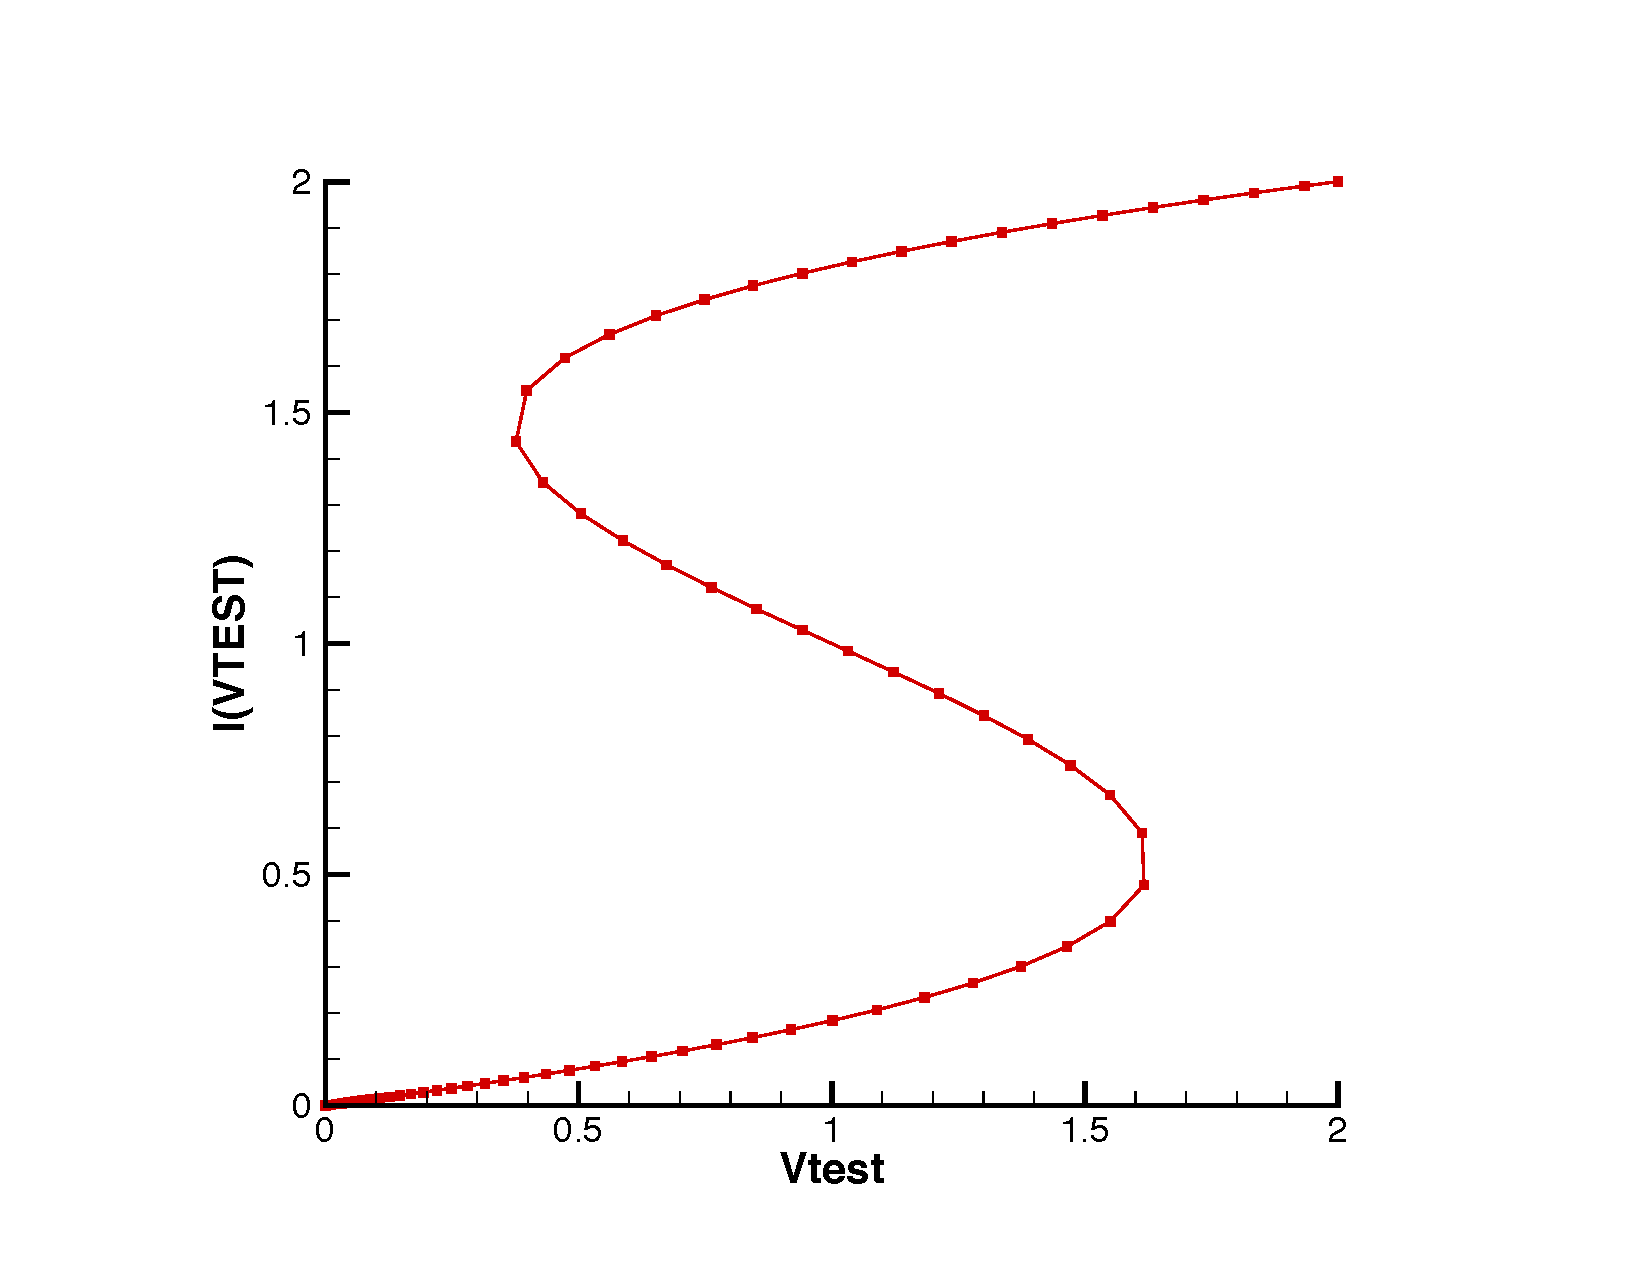
\includegraphics{arclengthSimple}}
  \caption [Arclength continuation example result. ]
  {Arclength continuation example result. This result was generated using \Xyce{} with the netlist in figure~\ref{arclength_netlist}.
\label{arclengthResult}
}
\end{figure}

\subsection{Explanation of Parameters, Best Practice}

Most of the parameters specified in the netlist~\ref{arclength_netlist} are 
the same as the ones described in the natural parameter 
section~\ref{locaParameterExplanation}.  However, two of them must be specified to non-default
values to enable an arclength calculation.   Specifically, the \texttt{stepper} 
parameter must be set to \texttt{1} or \texttt{ARC}, and the \texttt{predictor} 
parameter must be set to \texttt{2} or \texttt{SECANT}. 

%%% Local Variables:
%%% mode: latex
%%% End:

% END of Xyce_UG_ch10.tex ************

\cleardoublepage
%% Sandia National Laboratories is a multimission laboratory managed and
% operated by National Technology & Engineering Solutions of Sandia, LLC, a
% wholly owned subsidiary of Honeywell International Inc., for the U.S.
% Department of Energy’s National Nuclear Security Administration under
% contract DE-NA0003525.

% Copyright 2002-2020 National Technology & Engineering Solutions of Sandia,
% LLC (NTESS).

%%-------------------------------------------------------------------------
%% Purpose        : Time integration and MPDE info
%% Special Notes  : Graphic files (pdf format) work with pdflatex.  To use
%%                  LaTeX, we need to use postcript versions.  
%% Creator        : Richard Schiek, Electrical and Microsystem Simulation, SNL
%% Creation Date  : {05/16/2007}
%%
%%-------------------------------------------------------------------------

\chapter{Time Integration and Multi-time Partial Differential Equations (MPDE)}
\label{TimeInt}
\index{Time integration}
\index{MPDE}
\index{DAE}

\chapteroverview{Chapter Overview}
{
This chapter provides an overview and guidance on the time integration algorithms in \Xyce{},
Different time integration options can significantly effect simulation performance and accuracy.  
Additionally, this chapter provides an  overview and using instructions for the 
new Multi-Time Partial Differential Equation (MPDE) capability in \Xyce{}.
This chapter includes the following sections:
\begin{XyceItemize}
  \item Section~\ref{TimeInt}, {\em Differential Algebraic Equation (DAE) Time Integration}
  \item Section~\ref{MPDE_Overview}, {\em Multi-time Partial Differential Equations (MPDE) Overview}
  \item Section~\ref{MPDE_Usage}, {\em MPDE Usage}
\end{XyceItemize}
}

\section{Differential Algebraic Equation (DAE) Time Integration}
\label{TimeInt_Discussion}
\Xyce{} version 4.0 includes a major upgrade to the time integration capability.  
This upgrade will result in transient simulations running more accurately and with 
substantially fewer computed time steps.  This improved accuracy and efficiency comes at
a small cost, as more data structures must be maintained in the code to support this 
capability.  However, this cost has been minimized and the benefits of the new integrator
should be substantial.

The old time integrator was similar to that of Spice3f5, and its descendents.  Spice-style
integrators are based around older ordinary-differential-equation (ODE) 
integrators, which assume every equation in the system of equations include time derivatives.
In circuit problems, there are some fraction of the system of equations are purely algebraic.
For example, the KCL equation for a voltage node that has only linear resistors attached
to it is an algebraic equation, not a differential equation.  Systems of equations
that include some algebraic constraints are referred to as differential algebraic
equations (DAE), and such systems (as can be found in circuit simulation) are better served by 
time integrators that have been specifically designed for DAE's.  

Part of the reason for this is numerical stability.  Systems of DAE's are often characterized
by the DAE index, which is defined as ``the minimum number of times that all or part of [the DAE] 
must be differentiated with respect to $t$'' in order to reduce it to an ODE\cite{Petzold:1996}. 
A system of index=0 is an ODE system.  Many circuits have an index of 1 or more, and 
integrated MOSFET circuits usually have an index of at least 2~\cite{Brachtendorf1}.  This is important
because higher index systems are only stable and accurate for higher orders of 
integration, and are also very sensitive to initial conditions.
In contrast, an ODE (index=0) integrator has the luxury of assuming that any implicit 
time integration scheme will be stable.

\subsection{Solver Options and Guidance}

In general, from a user point of view, the switch to the new time integrator should be transparent,
and \Xyce{} version 4.0 should behave the same with previous \Xyce{} releases.  
Also, over the long term, the new time integrator should be a significant improvement over the old one.  
However, there
will be some rare exception circuits in which the new time integrator will have more difficulty than
the old one.  This is mostly due to the fact that the new time integrator hasn't been 
in the code long enough to be completely mature.  If a transient circuit that ran fine in previous 
releases does not run successfully in \Xyce{} version 4.0, there are several options available.

\begin{XyceItemize}
  \item Loosen the time integrator tolerances.  The default absolute and relative truncation error tolerances are the same as they were before, with the default abstol=1.0e-6 and the default reltol=1.0e-2.  The new time integrator will generally get accurate results with looser tolerances, because the integration scheme is inherently more accurate and less subject to numerical dispersion.  If a simulation exits with a time-step-too-small error, try using larger numbers for abstol and/or reltol.  For example:  \texttt{.options timeint abstol=1e-4 reltol=1e-2}.
  \item Change the maximum order.  In the old time integrator, the maximum integration order by default was 1.  In the new time integrator, the maximum order is, by default, 5.  In some cases, this will make the simulation less robust. It is possible to set the maximum order=1, in the netlist by adding \texttt{.options timeint maxord=1}.
\end{XyceItemize}


\section{Multi-time Partial Differential Equations (MPDE) Overview}
\label{MPDE_Overview}

\Xyce{} version 4.0 includes a new analysis option specially designed
for circuits with two disparate time scales.  Normally, when a circuit
has multiple time scales, the time integrator must take many small steps
to fully resolve the fast time scale which can greatly slow simulation
progress and reduce accuracy.  Now, \Xyce{} can discretize the system on
the fast time scale converting the fast time DAE to a multi-time partial
differential equation, hence MPDE.~\cite{meiMpdeDAC2004}  This dramatically
reduces the number of steps the time integrator must take resulting in a faster
and more accurate simulation.  

In general, best results will be obtained when there is a large
difference between the fast and slow time scales.  The quality of the
solution of the fast time scale depends on the number of points used
in the fast time discretization which also impacts simulation
performance. Typically, if one needs $n$ points to accurately discretize
the fast time scale, then the fast and slow time scales should be
separated by at least a factor of $n$, {\em i.e.} if one needed 10
points to represent the fast time solution, then best performance would
be found when the fast and slow time scales differ by at lest a factor
of 10.  In an MPDE analysis, \Xyce{} is effectively modeling $n$ versions of 
the simulated circuit, so memory usage will grow proportionally with the number 
of points in the fast time domain.

\section{MPDE Usage}
\label{MPDE_Usage}

To use MPDE analysis in a simulation, place the following option line in the 
netlist:

\noindent\texttt{.OPTIONS MPDE OSCSRC=<v1,v2...> IC=<1,2>} [other optional switches]

\begin{XyceItemize}

\item \texttt{OSCSRC=...} A list of voltage and, or current sources that are 
to be considered as changing on the fast time scale.  Typically these will 
be all the sources that change at or more quickly than the fast time scale.

\item \texttt{IC=[1,2]} Specifies the method used to calculate the
initial conditions for the MPDE problem.  1 uses the {\em Sawtooth}
algorithm while 2 uses an initial transient run for the initial
condition.  During the initial condition calculation, the slow sources
are deactivated so one is integrating only along the fast time axis.

\item \texttt{N2=integer} Specifies the number of equally spaced points 
to use in discretizing the fast time scale.  This option can only be used
exclusive of the \texttt{AUTON2} and \texttt{AUTON2MAX} options.

\item \texttt{AUTON2=[true | false]}  False by default.  If it is set to
true, then an initial transient run is done to generate a {\em mesh} of
time points for the fast time scale.  The belief here is that the time
integrator can do a better job picking out where it needs more points to
accurately describe the fast time solution.   Note: you can use
\texttt{AUTON2} with \texttt{IC=1} or texttt{IC=2}.  If you use it with
\texttt{IC=1}, then the time mesh is just used for the set of points the
for the Sawtooth initial conditions.  This option can only be used exclusive 
to the \texttt{N2} option.

\item \texttt{AUTON2MAX=integer}  This sets the maximum number of fast
time points that will be kept from the initial transient run so one has
some control over the size of the simulation.  If the initial transient
run produces 2,000 points and this is set at 50, \Xyce{} will uniformly
sample points from the solution set for the MPDE simulation. This option
can only be used exclusive to the \texttt{N2} option.

\item \texttt{STARTUPPERIODS=integer}  This is the number of fast time
periods that \Xyce{} should integrate through using normal transient analysis
before trying to generate initial conditions for the MPDE analysis. 

\item \texttt{diff=[0,1]}  Specifies the differentiation technique to use in 
calculating time derivatives on the fast time scale.  0 uses backward 
differences for the fast time differentiation while 1 uses central differences.

\end{XyceItemize}

As an example here are two valid options lines for MPDE:


\Example{\texttt{.options MPDE IC=1 N2=21 OSCSRC=Vsine}}
\Example{\texttt{.options MPDE IC=2 AUTON2=true AUTON2MAX=50 OSCSRC=VIN1,VIN2}}


%%% Local Variables:
%%% mode: latex
%%% End:

%% END of Xyce_UG_TimeInt.tex ************

% Sandia National Laboratories is a multimission laboratory managed and
% operated by National Technology & Engineering Solutions of Sandia, LLC, a
% wholly owned subsidiary of Honeywell International Inc., for the U.S.
% Department of Energy’s National Nuclear Security Administration under
% contract DE-NA0003525.

% Copyright 2002-2021 National Technology & Engineering Solutions of Sandia,
% LLC (NTESS).

%%-------------------------------------------------------------------------
%% Purpose        : Main LaTeX Xyce Users' Guide
%% Special Notes  : Graphic files (pdf format) work with pdflatex.  To use
%%                  LaTeX, we need to use postcript versions.  Not sure why.
%% Creator        : Scott A. Hutchinson, Computational Sciences, SNL
%% Creation Date  : {05/23/2002}
%%
%%-------------------------------------------------------------------------

\chapter{Results Output and Evaluation Options}
\label{Output}
\index{results!output options}

\chapteroverview{Chapter Overview}
{
This chapter illustrates how to output simulation results to data or output
files and includes the following sections:
\begin{XyceItemize}
  \item Section~\ref{Output_Control}, \nameref{Output_Control}
  \item Section~\ref{Additional_Output}, \nameref{Additional_Output}
  \item Section~\ref{Output_Analysis}, \nameref{Output_Analysis}
  \item Section~\ref{Results}, \nameref{Results}
\end{XyceItemize}
}

\section{Control of Results Output}
\label{Output_Control}
\index{results!output control}

\Xyce{} supports one solution output command, \texttt{.PRINT}, which is quite flexible, and supports several output formats.

\subsection{\texttt{.PRINT} Command}
\label{PRINT_section}
\index{output!\texttt{.PRINT}}

The \texttt{.PRINT} \index{\texttt{.PRINT}} command sends the analysis results to
an output file.  \Xyce{} supports several options on the \texttt{.PRINT} line of
netlists that control the format of the output. 

Multiple .PRINT lines may be present in the netlist.  Only .PRINT lines appropriate for the analysis being executed are
activated.  Each analysis type has a set of analysis print types.  These analysis print types are used to specify the variables
desired for each of the different output files which may be generated by an analysis type.  If an additional analysis print type is
activated and no .PRINT for that analysis print type is present, the variable list and options fall back to the .PRINT of that
analysis type.

\Format{\par\texttt{.PRINT <print type> [options] <output variable> [<output variable>]*}}

Table~\ref{Print_Types} lists the available print types for the analyses.

\begin{table}[!htb]
  \centering
  \caption[.PRINT Print Types]{.PRINT Print Types}
  \label{Print_Types}
  \index{results!print types} \index{\texttt{.PRINT}}
  % Sandia National Laboratories is a multimission laboratory managed and
% operated by National Technology & Engineering Solutions of Sandia, LLC, a
% wholly owned subsidiary of Honeywell International Inc., for the U.S.
% Department of Energy’s National Nuclear Security Administration under
% contract DE-NA0003525.

% Copyright 2002-2022 National Technology & Engineering Solutions of Sandia,
% LLC (NTESS).

{
\renewcommand{\arraystretch}{1.2}
\begin{tabular}{>{\ttfamily\small}m{1.5in}<{\normalfont}>{\ttfamily\small}m{0.75in}<{\normalfont}m{2.25in}@{}}
  \rowcolor{XyceDarkBlue}
  \color{white}\normalfont\bf Analysis &
  \color{white}\bf Print Type &
  \color{white}\bf Description \\
.AC & AC & Sets default variable list and formats for print subtypes \\ \hline
.AC & AC\_IC & Overrides variable list and format for AC initial conditions \\ \hline
.DC & DC &  \\ \hline
.EMBDEDDEDSAMPLING & ES & \\ \hline
.HB & HB & \\ \hline
.HB & HB\_FD & Overrides variable list and format for HB frequency domain \\ \hline
.HB & HB\_IC & Overrides variable list and format for HB initial conditions \\ \hline
.HB & HB\_STARTUP & Overrides variable list and format for HB start up \\ \hline
.HB & HB\_TD & Overrides variable list and format for HB time domain \\ \hline
.NOISE & Noise & Outputs Noise spectral density curves\\ \hline
.TRAN & TRAN &  \\ \hline
\multicolumn{3}{c}{\smallskip\color{XyceDarkBlue}\em\bfseries Specialized Output Commands} \\
\emph{Homotopy} & HOMOTOPY & Sets variable list and format for homotopy \\ \hline
.SENS & SENS & Sets variable list and format for sensitivity \\ \hline
\end{tabular}
}

\end{table}

Table~\ref{Print_Commands} gives the various options available to the
\texttt{.PRINT} command.  

\begin{table}[!htb]
  \caption[.PRINT command options.]{.PRINT command options.}
\label{Print_Commands}
  \index{results!print commands}
  \begin{tabularx}{\linewidth}{|>{\setlength{\hsize}{1.0\hsize}}Y|
      >{\setlength{\hsize}{1.0\hsize}}Y|}
    \rowcolor{XyceDarkBlue} \color{white}\bf Option\ldots &
    \color{white}\bf Action\ldots \\ \hline

    \texttt{FORMAT=}\newline \texttt{<STD|NOINDEX|PROBE|TECPLOT|RAW|CSV>} &
    Controls the output format.  See Table~\ref{Print_Format}.  The {\em
      default} is \texttt{STD}. \\ \hline

    \texttt{FILE=<filename>} & Output filename. The {\em default} is the
    netlist filename with ``\texttt{.prn}'' appended. \newline 
    \texttt{foo.cir.prn}, where \texttt{foo.cir} is the input netlist
  filename. The suffix depends on the format.  The {\em default} suffixes for \texttt{FORMAT=STD|PROBE|TECPLOT|RAW|CSV} 
  are ``\texttt{.prn}'', ``\texttt{.csd}'', ``\texttt{.dat}'', ``\texttt{.raw}'', and ``\texttt{.csv}'', respectively.  \\ \hline

    \texttt{WIDTH=<field-width>} & Column width for the output data \\ \hline

    \texttt{PRECISION=<floating-point-precision>} & Number of
    significant digits past the decimal point \\ \hline

    \texttt{FILTER=<floor-value>} & Absolute value below which output
    variables will be printed as 0.0 \\ \hline

    \texttt{DELIMITER=<TAB|COMMA>} & Alternate delimiter between columns
    of output in the \texttt{STD} output format. The default is spaces.\\ \hline

  \end{tabularx}

\end{table}

Table~\ref{Print_Format} gives the various output formats available to the
\texttt{.PRINT} command.  
\begin{table}[!htb]
  \caption[.PRINT FORMAT options.]{.PRINT FORMAT options.}
\label{Print_Format}
  \index{results!print format} \index{\texttt{.PRINT}!\texttt{FORMAT}}
  \begin{tabularx}{\linewidth}{|>{\setlength{\hsize}{1.0\hsize}}Y|
      >{\setlength{\hsize}{1.0\hsize}}Y|}
    \rowcolor{XyceDarkBlue} \color{white}\bf Format\ldots &
    \color{white}\bf Action\ldots \\ \hline

    \texttt{STD} & Outputs data in standard columns  \\ \hline
    \texttt{NOINDEX} & Outputs the same as the \texttt{STD} except the index column is omitted.  \\ \hline
    \texttt{PROBE} & Output is formatted to be compatible with the PSpice Probe plotting utility.  \\ \hline
    \texttt{RAW} & Output conforms to the Spice binary rawfile. Use the {\bf -a} command line option to produce an ASCII rawfile.  \\ \hline
    \texttt{TECPLOT} & Output for use in the TecPlot graphics package. \\ \hline
    \texttt{CSV} & Produces a comma-separated value format. \\ \hline
    \texttt{GNUPLOT} & Output data in standard columns, with improved Gnuplot compatibility for \texttt{.STEP} data. \\ \hline
  \end{tabularx}

\end{table}

The \texttt{<output variable>} parameter can be a variety of requested outputs,
including nodal voltages, {\tt V(...)}, or device currents, {\tt I(...)}, and power,
{\tt P(...)} or {\tt W(...)}, as given by
\begin{XyceItemize}
\item \texttt{V(<node name>)}
\item \texttt{V(<node name>,<node name>)} (the voltage difference between the first and second nodes)
\item \texttt{I(<two-terminal device>)}
\item \texttt{Ik(<three-or-more-terminal device>)} (the \texttt{k} indicates
  the device node from which to acquire the value, which is device specific;
  see the \Xyce{} Reference Guide\ReferenceGuide{} for details)
\item \texttt{P(two-terminal device)} 
\item \texttt{W(two-terminal device)}
\end{XyceItemize}

At this time, power calculations are only supported for {\tt .DC} and {\tt 
.TRAN} analysis types.  Power calculations may also not be supported for all \Xyce{}
devices yet.  Consult the \Xyce{} Reference Guide\ReferenceGuide{} for more details.
As an example, the power supplied or dissipated by the 
voltage source {\tt V} is calculated as $I \cdot \Delta V$ where the voltage drop is 
calculated as $(V_+ - V_-)$  and positive current flows from $V_+$ to $V_-$.  Dissipated power 
has a positive sign, while supplied power has a negative sign.  An important note is that
the power calculations are a post-processing step, which places a limit on the accuracy 
of circuit-wide ``energy conservation'' calculations (e.g., total power supplied by sources 
- total power dissipated in non-source devices) in \Xyce{}.  The accuracy of the inputs ({\tt V} and 
{\tt I}) to the power calculations is limited by the nonlinear solver tolerances, and the error
in the power calculations is upper-bounded by the sum of the product-terms of 
{\tt V*(error in I)} and {\tt I*(error in V)}.

Voltage variables specified in the frequency domain have special processing to
handle complex results.  For file formats which have a complex output
capability, the complex value is written.  However, for file formats, such as
STD and CSV, the complex value is written as two columns of data, the real part
followed by the imaginary part. Pseudo names may also be used to compute scalar
values from a complex voltage variable. These are given in
Table~\ref{Print_Complex}.

For {\tt .AC} and {\tt .NOISE} analyses, current variables (see Table~\ref{Print_Complex})
are only supported for devices that have ``branch currents'' that are part of the solution
vector.  This includes the V, E, H and L devices.  It also includes the voltage-form
of the B device.

\begin{table}[!htb]
  \caption{Pseudo Variables for Complex Output}
  \label{Print_Complex}
  \begin{tabularx}{\linewidth}{|Y|Y|}
    \rowcolor{XyceDarkBlue} \color{white}\textbf{Variable} & \color{white}\textbf{Definitions} \\ \hline
    \texttt{VR($node$)} & Voltage Real Component \\ \hline
    \texttt{VI($node$)} & Voltage Imaginary Component \\ \hline
    \texttt{VM($node$)} & Voltage Magnitude \\ \hline
    \texttt{VP($node$)} & Voltage Phase, Degrees \\ \hline
    \texttt{VDB($node$)} & Voltage Magnitude, Decibels \\ \hline
    \texttt{VR($node_1$,$node_2$)} & Difference of Voltage Real Component \\ \hline
    \texttt{VI($node_1$,$node_2$)} & Difference of Voltage Imaginary Component \\ \hline
    \texttt{VM($node_1$,$node_21$)} & Difference of Voltage Magnitude \\ \hline
    \texttt{VP($node_1$,$node_2$)} & Difference of Voltage Phase, Degrees \\ \hline
    \texttt{VDB($node_1$,$node_2$)} & Difference of Voltage Magnitude, Decibels \\ \hline
    \texttt{IR($device$)} & Current Real Component \\ \hline
    \texttt{II($device$)} & Current Imaginary Component \\ \hline
    \texttt{IM($device$)} & Current Magnitude \\ \hline
    \texttt{IP($device$)} & Current Phase, Degrees \\ \hline
    \texttt{IDB($device$)} & Current Magnitude, Decibels \\ \hline
    \texttt{SR($index_1$,$index_2$)} & S-Parameter Real Component \\ \hline
    \texttt{SI($index_1$,$index_2$)} & S-Parameter Imaginary Component \\ \hline
    \texttt{SM($index_1$,$index_2$)} & S-Parameter Magnitude \\ \hline
    \texttt{SP($index_1$,$index_2$)} & S-Parameter Phase, Degrees \\ \hline
    \texttt{SDB($index_1$,$index_2$)} & S-Parameter Magnitude, Decibels \\ \hline
    \texttt{YR($index_1$,$index_2$)} & Y-Parameter Real Component \\ \hline
    \texttt{YI($index_1$,$index_2$)} & Y-Parameter Imaginary Component \\ \hline
    \texttt{YM($index_1$,$index_2$)} & Y-Parameter Magnitude \\ \hline
    \texttt{YP($index_1$,$index_2$)} & Y-Parameter Phase, Degrees \\ \hline
    \texttt{YDB($index_1$,$index_2$)} & Y-Parameter Magnitude, Decibels \\ \hline
    \texttt{ZR($index_1$,$index_2$)} & Z-Parameter Real Component \\ \hline
    \texttt{ZI($index_1$,$index_2$)} & Z-Parameter Imaginary Component \\ \hline
    \texttt{ZM($index_1$,$index_2$)} & Z-Parameter Magnitude \\ \hline
    \texttt{ZP($index_1$,$index_2$)} & Z-Parameter Phase, Degrees \\ \hline
    \texttt{ZDB($index_1$,$index_2$)} & Z-Parameter Magnitude, Decibels
  \end{tabularx}
\end{table}

In addition to the above, internal device variables can be specified as an
\texttt{<output variable>}.  These take the form, \texttt{N(device variable)}.
The format of the \texttt{device variable} called by \texttt{N} is
device-specific, and exact forms can be found in the \Xyce{} Reference
Guide\ReferenceGuide{}.

It is also possible to output a device or model parameter directly, such as 
the resistance of a resistor \texttt{R5}, specified as \texttt{R5:R} on the \texttt{.PRINT} line.
It is necessary to specify both the device name and parameter name,
separated by a colon.

Finally, an expression may also be specified as an \texttt{<output
variable>}. To do so, enclose the expression within curly braces
(\texttt{\{\}}).  See Section~\ref{Parameters_Expressions} for a description of
expressions.

\Example{\\
\texttt{.PRINT TRAN FILE=Output.prn V(3) I(R3) ID(M5) V(4)} \\
\texttt{.PRINT DC FORMAT=TECPLOT FILE=Output.dat V(2) \{I(C3)+abs(V(4))*5.0\}} \\  
\texttt{.PRINT HB RA:R V(Vsrc) VM(Vsrc)} \\
\texttt{.PRINT HB\_TD RA:R V(Vsrc)} \\
\texttt{.PRINT TRAN FORMAT=CSV R1:R R1:TEMP I(R1) R2:R R2:TEMP} \\
\texttt{.PRINT AC v(3)} 
\texttt{.PRINT AC FILE=AUX.FD.prn v(1)} 
\texttt{.OP \newline .PRINT AC\_IC v(1) v(2)} 
}

\newpage
\subsection{Additional Output Options}
\label{Additional_Output}

Additional control of \texttt{.PRINT} line output can be set using the 
\texttt{.OPTIONS OUTPUT} specification.
\index{\texttt{.OPTIONS}!\texttt{OUTPUT}}

\subsubsection{Output Intervals}
An important feature of the \texttt{.OPTIONS OUTPUT} command is to provide 
control of the interval at which transient data is written to files specified by 
\texttt{.PRINT TRAN} commands.  This can be
especially useful in controlling the size of the results file for
simulations that require a large number of time steps.  
The default behavior is for \Xyce{} to output results at every time step, so 
using this feature to reduce output frequency will result in improved performance.
\index{\texttt{.PRINT}!\texttt{TRAN}}
\index{results!output interval}

\index{\texttt{.OPTIONS}!\texttt{OUTPUT}!\texttt{INITIAL\_INTERVAL}}
\Format{\par\texttt{.OPTIONS OUTPUT INITIAL\_INTERVAL=<interval> [<t0>
      <i0> [<t1> <i1> ...]]}}

\texttt{INITIAL\_INTERVAL=<interval>} specifies the starting interval time
for output and \texttt{<tx ix>} specifies later simulation times (\texttt{tx})
where the output interval will change to (\texttt{ix}).

The following example shows the output being requested (via the netlist
\texttt{.OPTIONS OUTPUT} command) every .1$\mu s$ for the first 10$\mu s$,
every 1$\mu s$ for the next 10$\mu s$, and every 5$\mu s$ for the remainder of
the simulation:

\Example{\texttt{.OPTIONS OUTPUT INITIAL\_INTERVAL=.1us 10us 1us 20us 5us}}

\subsubsection{Suppressing output file header and footer}

\index{\texttt{.OPTIONS}!\texttt{OUTPUT}!\texttt{PRINTHEADER}}
\index{\texttt{.OPTIONS}!\texttt{OUTPUT}!\texttt{PRINTFOOTER}}
It can be convenient to have an output file that contains only numerical data with 
minimal formatting.  There are two options,\texttt{PRINTHEADER} and \texttt{PRINTFOOTER} 
available on the \texttt{.OPTIONS OUTPUT} line to facilitate this. The format
is given by:

\Format{\par\texttt{.OPTIONS OUTPUT PRINTHEADER=<boolean>  PRINTFOOTER=<boolean> }}
So, to produce an output file that has no header and no footer, simply set:

\Example{\texttt{.OPTIONS OUTPUT PRINTHEADER=false PRINTFOOTER=false}}
Note that \texttt{PRINTHEADER} is only supported for \texttt{.PRINT FORMAT=<STD|GNUPLOT|SPLOT>},
while \texttt{PRINTFOOTER} is only supported for \texttt{.PRINT FORMAT=<STD|GNUPLOT|SPLOT|TECPLOT>}.

\subsection{Output File Redirection}
There are three ways to re-direct the output of a \Xyce{} simulation run
to a file other than the default file.  They are the \verb+-r+ and 
\verb+-o+ command line options and the \texttt{FILE=} qualifier on  
individual \texttt{.PRINT} lines.  This subsection provides an overview of 
them, and how they work with each other. 

\subsubsection{-r Output}
The \verb+-r <fileName>+ command line option will output all of the variables 
in the solution vector to the binary rawfile \verb+<fileName>+.  The
command line \verb+-r  <fileName> -a+ will output a human-readable (ASCII) 
rawfile instead.  The \verb+-r+ command line option is supported for the
\texttt{.AC}, \texttt{.DC}, \texttt{.NOISE} and \texttt{.TRAN} analysis
types.  

If the \verb+-r+ and \verb+-o+ command line options are both specified then 
the \verb+-r+ command line option takes precedence. Also, \Xyce{} does not
permit the \verb+-r+ output to overwrite the netlist file (\verb+<netlistName>+).
Instead, the output will be placed into the file \verb+<netlistName>.raw+.

If \verb+-r+ output is requested for a netlist that has \texttt{.PRINT SENS}
or \texttt{.PRINT HOMOTOPY} lines in it then the sensitivity and homotopy
output will use the instructions given by those \texttt{.PRINT} lines.  This
approach was taken because those two analysis types do not support rawfile 
output.  However, an attempt to re-direct the sensitivity and homotopy output,
with a \texttt{FILE=} qualifier on their \texttt{.PRINT} lines, to the same file
as requested with the \verb+-r <fileName>+ command line option will be a
fatal parsing error.

\subsubsection{-o Output}
The \verb+-o+ command line option is supported for compatibility with other
circuit simulators such as Spice3f5.  As mentioned above, if the \verb+-r+ and 
\verb+-o+ command line options are both specified then the \verb+-r+ command 
line option will take precedence.  Also, \Xyce{} does not permit the \verb+-o+ output 
to overwrite the netlist file (\verb+<netlistName>+).  Instead, the output will 
be placed into the file \verb+<netlistName>.prn+. 

The \verb+-o <fileName>+ command line option is supported for the \texttt{.AC}, 
\texttt{.DC}, \texttt{.HB}, \texttt{.NOISE} and \texttt{.TRAN} analysis 
types.  The output file (\verb+<fileName>+) will be in \texttt{FORMAT=STD} with
spaces as the delimiter between columns.  So, the \verb+-delim+ command line 
option and any \texttt{DELIMITER=}, \texttt{FILE=} and \texttt{FORMAT=}
qualifiers on the relevant \texttt{.PRINT} lines will be silently ignored. 

For the \verb+-o+ command line option, the variable list in the output file 
(\verb+<fileName>+) will be the ``concatentation'' of the variable lists from
all of the relevant \texttt{.PRINT} lines in the netlist.  So, for a 
\texttt{.TRAN} simulation the variable list will come from all of the 
\texttt{.PRINT TRAN} lines in the netlist.  The behavior for \texttt{.AC} and 
.\texttt{.HB} analyses is slightly different.  For a \texttt{.AC} analysis, 
the variable list will come from all of the \texttt{.PRINT AC} lines in the 
netlist.  Any variables listed on the \texttt{.PRINT AC\_IC} lines will not 
be included.   For a \texttt{.HB} analysis, the variable list will come from 
all of the \texttt{.PRINT HB} and \texttt{.PRINT HB\_FD} lines in the netlist.  
Any variables listed on the \texttt{.PRINT HB\_TD}, \texttt{.PRINT HB\_IC} and
\texttt{.PRINT HB\_STARTUP} lines will not be included.

As mentioned above, the \verb+-o+ command line option will not produce 
any output from \texttt{.PRINT AC\_IC}, \texttt{.PRINT HB\_TD}, 
\texttt{.PRINT HB\_IC} and \texttt{.PRINT HB\_STARTUP} lines.  In addition,
it will not produce any output from \texttt{.PRINT SENS} or 
\texttt{.PRINT HOMOTOPY} lines.

\subsubsection{FILE= Qualifier on .PRINT Lines}
The \texttt{FILE=<fileName>} qualifier on individual \texttt{.PRINT} lines is
often a preferred option to the \verb+-o+ command line option for output file 
redirection, since it is more flexible.  However, as noted above, the \verb+-r+
 and \verb+-o+ command line options do take precedence if either of them are 
specified.

The combination of \texttt{FILE=} and \texttt{FORMAT=} qualifiers on the 
\texttt{.PRINT} lines in a netlist allows fine-grained control of the 
output formats, output file names and variable lists in each file.  As a 
simple example, this combination of \texttt{.PRINT lines} would produce output
files in both \texttt{PROBE} (\verb+<netlistName.csd>+) and \texttt{CSV}
(\verb+<netlistName.csv>+) formats without having to do multiple simulation runs.

\begin{verbatim}
.PRINT TRAN FORMAT=CSV V(1) V(2)
.PRINT TRAN FORMAT=PROBE V(1) V(2) 
\end{verbatim}

Finally, \Xyce{} does not permit the \texttt{FILE=} qualifier to overwrite the 
netlist file (\verb+<netlistName>+).  Instead, the output will be placed into 
the file \verb+<netlistName>.<defaultExtension>+, where the default extension
is set by  the \texttt{FORMAT=} qualifier on that \texttt{.PRINT} line and the 
analysis type specified in the netlist.

\subsubsection{Multi-File Output for AC and HB Analysis}
The {\tt .AC} and {\tt .HB} analysis types can produce multiple output files.
This can occur in two ways.  For example, a netlist may have explicit
\texttt{.PRINT HB\_FD} and \texttt{.PRINT HB\_TD} lines.  In that case, the
frequency domain and time domain outputs for that netlist's {\tt .HB} analysis 
will use the explicit variable lists, \texttt{FILE=} qualifiers, and \texttt{FORMAT=} 
qualifiers from each line.  As a convenience, \Xyce{} can also generate
``fallback print lines''.  For example, a \texttt{.PRINT HB} will 
automatically generate the output from equivalent \texttt{.PRINT HB\_FD} 
and \texttt{.PRINT HB\_TD} lines using its variable list, \texttt{FILE=} qualifier, 
and \texttt{FORMAT=} qualifier.  

The interactions and precedence between these types of output are as follows.  
First, a more explicit line (e.g., \texttt{.PRINT HB\_FD} or 
\texttt{.PRINT AC\_IC}) takes precedence over a less explicit line (e.g., 
\texttt{.PRINT HB} or \texttt{.PRINT AC}), if both appear in the netlist.
Second, if a \texttt{FILE=hbFile} qualifier appears on a \texttt{.PRINT HB}
line, that is using \texttt{FORMAT=STD}, then its four possible output files 
will be \texttt{hbFile.HB.FD.prn}, \texttt{hbFile.HB.TD.prn},
\texttt{hbFile.hc\_ic.prn} and \texttt{hbFile.startup.prn}.  Finally, if a
\texttt{FILE=acFile} qualifier appears on a \texttt{.PRINT AC} line, that 
is using \texttt{FORMAT=STD}, then its two possible output files will 
be \texttt{acFile} and \texttt{acFile.TD.prn}.    
  
\section{Output Analysis}
\label{Output_Analysis}

\subsection{.MEASURE}
\index{results!measure} \index{\texttt{.MEASURE}}
\label{measure}
\Xyce{} supports analysis of the data from a simulation through the
\texttt{.MEASURE} command.  Using \texttt{.MEASURE} one can locate extrema in a
voltage or current node, calculate integrals, derivatives, Fourier transforms,
and locate transient events. (Note: \texttt{.MEAS} is an allowed synonym for 
\texttt{.MEASURE} in \Xyce{}.)
\Format{\par\texttt{.MEASURE <analysis type> <measure name> <measure type>
<simulation variable> \newline + [qualifiers]}}
\texttt{<analysis type>} is the analysis under which the measure should be calculated.  
Currently,  transient (\texttt{.TRAN}), dc (\texttt{.DC}), ac (\texttt{.AC})
and noise (\texttt{.NOISE}) analyses
are supported, and \texttt{.MEASURE} can be used with \texttt{.STEP} in all four cases.
The specified measure is referenced by \texttt{<measure name>}.  That name is used 
in the summary output at the end of the simulation to report the value of that
measure, and can also be used in \texttt{.PRINT} statements.  The
\texttt{<measure type>} is the type of calculation to be done.  For \texttt{.TRAN}
analyses, the supported measure types are:
\begin{XyceItemize}
\item \texttt{AVG}: Computes the arithmetic mean.
\item \texttt{DERIV}: Computes the derivative of a simulation variable, either at a user-specified
    time or when the simulation variable hits a user-specified value.
\item \texttt{DUTY}: Fraction of time that a given simulation variable is greater than \texttt{ON} and 
    does not fall below \texttt{OFF} (\texttt{ON} and \texttt{OFF} are defined later in this section).
 \item \texttt{EQN}: Calculates the value of a \Xyce{} expression during the simulation.
 \item \texttt{ERR, ERR1 and ERR2}: Calculate the error between simulation variables.
 \item \texttt{ERROR}: Calculates the norm between the measured waveform and a ``comparison
    waveform'' specified in a file.  The supported norms are L1, L2 and INFNORM.  The
    default norm is the L2 norm.  The descriptive output for each ERROR measure,
    that is printed to standard output, will explicitly state which norm  was used for 
    each ERROR measure.
 \item \texttt{FIND-AT}: Returns the value of a solution variable when the independent variable
    (time, frequency or DC sweep value) reaches the value specified in the \texttt{AT} clause.
    If the conditions specified in the \texttt{AT} clause are not found during the simulation
    then the measure will return the default value of -1 (or the user-specified default value).
 \item \texttt{FIND-WHEN}: Returns the value of a solution variable when the solution variable specified 
    in the \texttt{WHEN} clause reaches a specified fixed value or is equal to another solution variable.  
    If the conditions specified for finding the value specified in the \texttt{WHEN} clause are not found 
    during the simulation then the measure will return the default value of -1 (or the user-specified 
    default value).
  \item \texttt{FOUR}: Calculates the Fourier transform of the solution variable for the \texttt{.TRAN}
    analysis type using the fundamental frequency \texttt{AT}.  By default, the DC component 
    and first nine harmonics are computed; more can be reported by setting \texttt{NUMFREQ} to the
    desired value.  More interpolation points can be used in the Fourier analysis by setting \texttt{GRIDSIZE},
    which is $200$ by default.  For this measure, the phase data is output in degrees.
  \item \texttt{FREQ}: An estimate of the frequency of a solution variable found by cycle counting
    during the simulation.  Thresholds are defined through the values of \texttt{ON} 
    and \texttt{OFF}.
  \item \texttt{INTEG}: Calculates the integral of a solution variable through second order numerical 
    integration.
  \item \texttt{MAX}: Returns the maximum value of a solution variable.
  \item \texttt{MIN}: Returns the minimum value of a solution variable.
  \item \texttt{OFF\_TIME}: Returns the time that a solution variable is below \texttt{OFF}, and not
    greater than \texttt{ON} for the simulation, normalized by the number of cycles
of the waveform during the simulation.
  \item \texttt{ON\_TIME}: Returns the time that a solution variable is above \texttt{ON}, and not
    less than \texttt{OFF} for the simulation, normalized by the number of cycles
of the waveform during the simulation.
  \item \texttt{PP}: Returns the difference between the maximum value and the minimum value of
    a solution variable during the simulation.
  \item \texttt{RMS}: Computes the root-mean-squared value of a solution variable.
  \item \texttt{TRIG-TARG}: Measures the time between a trigger event and a target event.
  \item \texttt{WHEN}: Returns the time when a solution variable reaches a specified fixed 
    value or is equal to another solution variable.  If the conditions specified for
    finding the value specified in the \texttt{WHEN} clause are not found during the simulation 
    then the measure will return the default value of -1 (or a user-specified default value).
\end{XyceItemize}

The \texttt{AVG}, \texttt{DERIV}, \texttt{EQN},   \texttt{ERR},  \texttt{ERR1}, \texttt{ERR2},
\texttt{FIND-AT}, \texttt{FIND-WHEN}, \texttt{INTEG}, \texttt{MIN}, \texttt{MAX}, \texttt{PP},
\texttt{RMS} and \texttt{WHEN} measures are supported for all four ``measure modes'' (\texttt{TRAN},
\texttt{DC}, \texttt{AC} and \texttt{NOISE}).  The \texttt{TRIG-TARG} measure is only supported for
\texttt{TRAN} measure mode.  

The \texttt{ERROR} measure is \Xyce{}-specific, and is only supported for \texttt{TRAN} and
\texttt{DC} measure modes.  The \texttt{DUTY}, \texttt{FREQ}, \texttt{FOUR}, \texttt{OFF\_TIME}
and \texttt{ON\_TIME} measures are also \Xyce{}-specific, and are  only supported for
\texttt{TRAN} measure mode.

\Xyce{} also supports ``continuous'' measures, that can return more than one value, for
\texttt{.TRAN}, \texttt{.DC}, \texttt{.AC} and \texttt{.NOISE} analyses.  The
 corresponding measure modes are \texttt{TRAN\_CONT}, \texttt{DC\_CONT},
\texttt{AC\_CONT} and \texttt{NOISE\_CONT}.  The supported measure types for continuous
measures are \texttt{DERIV-AT}, \texttt{DERIV-WHEN}, \texttt{FIND-AT}, \texttt{FIND-WHEN}
and \texttt{WHEN} measures.  Continuous measure modes are not supported for \texttt{TRIG}
or \texttt{TARG} measures.

For transient analyses, that also have \texttt{.FFT} analysis statements, \Xyce{} also
supports \texttt{FFT} measure mode.  In that case, the following additional measure
types can be associated with those \texttt{.FFT} lines.  In addition, \texttt{FFT}
mode measures, such as \texttt{FIND-AT} measures, can be used in \texttt{EQN} measures
to create more customized metrics from the \texttt{.FFT} results.

\begin{XyceItemize}
  \item \texttt{ENOB}: computes the Effective Number of Bits.
  \item \texttt{FIND-AT}: returns the requested FFT cofficient at the
     requested frequency, which is rounded to the nearest harmonic.
  \item \texttt{SFDR}: computes the Spurious Free Dynamic Range.
  \item \texttt{SNDR}: computes the Signal to Noise-plus-Distortion Ratio.
  \item \texttt{SNR}: computes the Signal to Noise Ratio.
  \item \texttt{THD}: computes the Total Harmonic Distortion.
\end{XyceItemize}

The \texttt{<simulation variable>} specifies a voltage or current node that
will be used in this measure, such as \texttt{V(a)}.  The measure \texttt{WHEN}
is different from the other measures in that it can take one or two solution
variables. For example, \texttt{WHEN v(a)=5} returns the time when
\texttt{V(a)} equals 5.  Or, if \texttt{WHEN V(a) = V(b)} is specified, the
time when \texttt{V(a)} equals \texttt{V(b)} is returned.

The \texttt{.MEASURE} command can also take optional \texttt{[qualifiers]} that
limit the time window (or frequency window or DC sweep values) when \texttt{.MEASURE} is 
applied. The \texttt{[qualifiers]} also place numeric limits on what state a value is
considered to be in (e.g., \texttt{ON} and \texttt{OFF}), and provide numeric
qualification on comparisons of values (e.g., \texttt{MINVAL}).  A partial list of the supported
qualifiers is as follows.  See the \Xyce{} Reference Guide\ReferenceGuide{} for more details
on these qualifiers, and for the complete list of supported qualifiers for each combination
of analysis type and measure type.

\begin{XyceItemize}
\item \texttt{FROM=value} A time (or frequency or DC sweep value) after which the 
measurement calculation will start.

\item \texttt{TO=value} A time (or frequency or DC sweep value) after which the 
measurement calculation will end.

\item \texttt{TD=value} A time delay before which the measurement should be taken or checked.

\item \texttt{RISE=r|LAST}  The number of rises after which the measurement should be checked.  If
\texttt{LAST} is specified, then the last rise found in the simulation will be used.

\item \texttt{FALL=f|LAST}
  The number of falls after which the measurement should be checked.  If
  \texttt{LAST} is specified, then the last fall found in the simulation
  will be used.

\item \texttt{CROSS=c|LAST} 
  The number of zero crossings after which the measurement should be checked.  If
  \texttt{LAST} is specified, then the last zero crossing found in the simulation
  will be used.

\item \texttt{MINVALUE=value}
  An allowed absolute difference between the simulation variable and the variable
  to which it is being compared.  This has a default value of 1.0e-12.  One 
  may need to specify a larger value to avoid missing the test condition
  in a transient run.

\item \texttt{ON=value}
  The value at which a signal is considered to be on for frequency, duty and
  on time calculations

\item \texttt{OFF=value}
  The value at which a signal is considered to be off for frequency, duty and
  off time calculations.

\end{XyceItemize}

An example of using \texttt{.measure } during a transient analysis is shown in the following netlist:

\begin{verbatim}
VS  1  0  SIN(0 1.0 1KHZ 0 0)
VP  2  0  PULSE( 0 1 0.2ms 0.2ms 0.2ms 1ms 2ms )

R1  1  0  100
R2  2  0  100

.TRAN 0  10ms
.PRINT TRAN FORMAT=NOINDEX V(1) V(2) 

.MEASURE TRAN avg1 AVG V(1)
.MEASURE TRAN avg2 AVG V(2)

.MEASURE TRAN duty1 DUTY V(1) ON=0.75 OFF=0.25

\end{verbatim}

The measure \texttt{avg1} returns the average of \texttt{v(1)}, and
\texttt{avg2} returns the average of \texttt{v(2)}. Additionally,
\texttt{duty1} computes the fraction of time that \texttt{v(1)} is above
0.75~V, without falling below 0.25~V. 

The next netlist provides an example of using the \texttt{when} measure
during a transient analysis:

\begin{verbatim}
VS  1  0  SIN(0 1.0 1KHZ 0 0)
VP  2  0  PULSE( 0 100 0.2ms 0.2ms 0.2ms 1ms 2ms )

R1  1  0  100
R2  2  0  100

.TRAN 0  10ms 0 1.0e-5
.PRINT TRAN FORMAT=NOINDEX V(1) V(2) 

.MEASURE TRAN hit1_75 WHEN V(1)=0.75 MINVAL=0.02
.MEASURE TRAN hit2_75 WHEN V(1)=0.75 MINVAL=0.08 RISE=2

\end{verbatim}

In the above netlist, the measure called \texttt{hit1\_75} will return the
simulation time where \texttt{v(1)} reaches a value of 0.75, while {\tt
hit2\_75} returns the second time that \texttt{v(1)} reaches a value of 0.75.
The \texttt{MINVAL} option acts at an absolute tolerance in this case. So, the
above measure statements are more exactly interpreted as \texttt{hit1\_75} is
the simulation time when \texttt{v(1)} reaches a value of $0.75 \pm 0.02$ and
\texttt{hit2\_75} is the simulation time when {\tt v(1)} reaches a value of
$0.75 \pm 0.08$ on its second rise.

Measured results are reported to the output and log file.  Additionally, for \texttt{TRAN}
measures, the results are stored in files called \texttt{circuitFileName.mt\#}, where
the suffixed number (\texttt{\#}) starts at \texttt{0} and increases for multiple
iterations (\texttt{.STEP} iterations) of a given simulation. Each line of this file
will contain the measurement name, followed by its value for that run and/or step 
iteration.  For \texttt{DC} measures, the results are stored in the files
\texttt{circuitFileName.ms\#}, while \texttt{AC} and \texttt{NOISE} measures
use the files \texttt{circuitFileName.ma\#}.

\Xyce{} also supports an ability to {\it re-measure} results from a prior run of \Xyce{}.
In this mode, one can modify \texttt{.MEASURE} and/or \texttt{.FFT} statements and have
\Xyce{} recalculate  the results based on existing simulation data.  This can be useful if the
original simulation takes some time to complete.  (Note: \texttt{remeasure} works for both
transient and dc analyses.  However, it may be most useful for transient analyses.  It is
not currently supported for ac or noise analyses.)  The syntax in the netlist is the same
and the only thing that changes is how one invokes \Xyce{}.  For example, if the netlist
is called {\tt myNetlist.cir} and the existing output file is called {\tt myNetlist.cir.prn},
then remeasure is accomplished with:
{\tt
\begin{verbatim}
Xyce -remeasure myNetlist.cir.prn myNetlist.cir
\end{verbatim}
}

There are some important limitations to \texttt{remeasure}.  First, the data used by the
\texttt{.MEASURE} and/or \texttt{.FFT} commands must be present in the output file because,
in this mode, \Xyce{} is not recalculating the full solution.  Second,\texttt{.prn},
\texttt{.csv} and \texttt{.csd} files are supported, but remeasure may only
work for \texttt{.csv} and \texttt{.csd} files generated by \Xyce{}.


\subsection{.FOUR}
\index{results!four}\index{\texttt{.FOUR}}
Fourier analysis can be performed as a part of the transient analysis using
the \texttt{.FOUR} command.
\Format{\par\texttt{.FOUR freq ov1 <ovn>*}}


\texttt{freq} is the fundamental frequency used for Fourier analysis.
The \texttt{ov1} parameter is the desired solution output to be analyzed, specifically:
\begin{XyceItemize}
\item \texttt{V(<node name>)}
\item \texttt{V(<node name>,<node name>)} (the voltage difference between the first and second nodes)
\item \texttt{I(<two-terminal device>)}
\item \texttt{Ik(<three-or-more-terminal device>)} (see the \texttt{.PRINT} section, \ref{PRINT_section}, for more detail)
\item \texttt{N(device variable)} (see the \texttt{.PRINT} section, \ref{PRINT_section}, for more detail)
\item \texttt{SENS} Transient direct sensitivities specified by the \texttt{.SENS} command  (see the sensitivity analysis section, \ref{SENS_Analysis} for more detail)
\item The pseudo-variables given in Table~\ref{Print_Complex} for complex output handling
\end{XyceItemize}
At least one solution variable must be specified, but
Fourier analysis can be performed on several solution variables for each 
fundamental frequency, \texttt{freq}.
Multiple \texttt{.FOUR} lines may be used in a netlist.  
All results from Fourier analysis will be returned to the user in a file 
with the same name as the netlist file suffixed with \texttt{.four}.
For this analysis, the phase data is output in degrees.

If \texttt{SENS} is specified as the output, then all the direct sensitivities 
specified by the \texttt{.SENS} command will be processed, as it is difficult to 
manually specify the full name of a sensitivity variable.  So, if one wants 
to use sensitivities as the output, do the following:
\begin{verbatim}
.FOUR 20MEG SENS
\end{verbatim}

Fourier analysis is performed over the last period (\texttt{1/freq}) of 
the transient simulation.  The dc component and the first nine harmonics are calculated.
The number of harmonics computed by \texttt{.FOUR} is static.  So, the
main difference between \texttt{.FOUR} and the Fourier analysis in \texttt{.MEASURE} is that the latter allows the user to select the number of harmonics.  
The default options for the Fourier analysis in \texttt{.MEASURE} 
is the same as \texttt{.FOUR}.  For instance, these two lines will result in the 
same Fourier analysis:

\begin{verbatim}
.FOUR 20MEG V(2)
.MEASURE TRAN FOURV2 FOUR V(2) AT=20MEG
\end{verbatim}


The Fourier analysis in \texttt{.MEASURE} will allow for more harmonics
to be computed using the \texttt{NUMFREQ} option and more interpolation points
to be used in the Fourier analysis with \texttt{GRIDSIZE}.  
For instance, to compute twenty harmonics
(including the dc component), the previous \texttt{.MEASURE} line can be amended to:

\begin{verbatim}
.MEASURE TRAN FOURV2 FOUR V(2) AT=20MEG NUMFREQ=20
\end{verbatim}

To increase the number of interpolation points from $200$, which is the default,
to $500$, the line can be amended to:

\begin{verbatim}
.MEASURE TRAN FOURV2 FOUR V(2) AT=20MEG NUMFREQ=20 GRIDSIZE=500
\end{verbatim}

For maximum accuracy of the Fourier analysis, it is recommended that 
the time integration option \texttt{DELMAX}
should be set to \texttt{period/100}.  This is the preferred approach to
improving the accuracy of the Fourier analysis versus increasing the number of
interpolation points.

\subsection{.FFT}
\index{results!fft}\index{\texttt{.FFT}}
A Fast Fourier Transform (FFT) analysis can be performed as a part of the
transient analysis using the \texttt{.FFT} command.  The simplest
invocation would be:
\Format{\par\texttt{.FFT <ov>}}

where the \texttt{ov1} parameter is the desired solution output to be analyzed, specifically:
\begin{XyceItemize}
\item \texttt{V(<node name>)}
\item \texttt{V(<node name>,<node name>)} (the voltage difference between the first and second nodes)
\item \texttt{I(<two-terminal device>)}
\item \texttt{Ik(<three-or-more-terminal device>)} (see the \texttt{.PRINT} section, \ref{PRINT_section}, for more detail)
\item \texttt{N(device variable)} (see the \texttt{.PRINT} section, \ref{PRINT_section}, for more detail)
\end{XyceItemize}

Other useful optional parameters include the following:
\begin{XyceItemize}
  \item{\texttt{NP=value}} The number of points in the FFT.  This value must be a power of 2.
     The default value is 1024.
  \item{\texttt{WINDOW=value}} The windowing function that will be applied to the sampled waveform
values.  The allowed values are as follows:
    \begin{itemize}
      \item \texttt{RECT} = rectangular window (default)
      \item \texttt{BART} = Bartlett (triangular) window
      \item \texttt{HANN} = Hanning window
      \item \texttt{HAMM} = Hamming window
      \item \texttt{BLACK} = Blackman window
      \item \texttt{HARRIS} = Blackman-Harris window
    \end{itemize}
  \item{\texttt{START=value}} The start time for the FFT analysis. The default value is the
start time for the transient analysis.
  \item{\texttt{STOP=value}} The end time for the FFT analysis. The default value is the
end time for the transient analysis.
\end{XyceItemize}

The \Xyce{} Reference Guide\ReferenceGuide{} provides more details on these
optional parameters, as well as additional ones.

For maximum accuracy of the FFT analysis, it is recommended that the default
setting of \texttt{.OPTIONS FFT FFT\_ACCURATE=1} be used.  This setting instructs
\Xyce{} to insert breakpoints at the sample times requested by the collection of
\texttt{.FFT} statements in the netlist.  In addition, the optional metrics for
each \texttt{.FFT} line can be sent to stdout by setting \texttt{.OPTIONS FFT FFTOUT=1}.
Those metrics include the Effective Number of Bits (ENOB), Spurious Free Dynamic
Range (SFDR), Signal to Noise Ratio (SNR), Signal to Noise-and-Distortion Ratio (SNDR)
and Total Harmonic Distorion (THD).  The \Xyce{} Reference Guide\ReferenceGuide{}
provides detailed definitions for these metrics.  It also discusses the compatibility
of various \texttt{.OPTIONS OUTPUT} and \texttt{.OPTIONS FFT} settings.

\Xyce{} also supports an ability to {\it re-measure} results from a prior run of \Xyce{}.
In this mode, one can modify \texttt{.MEASURE} and/or \texttt{.FFT} statements and have
\Xyce{} recalculate the results based on existing simulation data.  Section \ref{measure}
and the \Xyce{} Reference Guide\ReferenceGuide{} provides more details on this capability.

\section{Graphical Display of Solution Results}
\label{Results}
\index{results!graphing}
Although \Xyce{} does not provide integrated graphical display options,
it produces output in a form that may readily be used with commonly
available graphical tools, including TecPlot, gnuplot, and MS Excel (see
figure~\ref{Clipper_TP} for an example plot using TecPlot,
\texttt{http://www.amtec.com}).  The standard \Xyce{} print format
(\texttt{FORMAT=STD} or \texttt{FORMAT=NOINDEX}) is well suited for
use with gnuplot.  However, \texttt{FORMAT=GNUPLOT} may be useful when 
plotting \texttt{.STEP} data in gnuplot, as it automatically inserts two 
blank lines between the blocks of step-data that are otherwise in 
standard format.  Comma separated variable (\texttt{FORMAT=CSV}) is
the best choice for import into Excel.  \texttt{FORMAT=TECPLOT}
produces output specifically targeted at the TecPlot tool. 
The \texttt{FORMAT=PROBE}\index{\texttt{.PRINT}!\texttt{FORMAT}}
option to the \texttt{.PRINT} command produces output
\texttt{.csd} files that can be read by the PSpice
Probe\index{PSpice!Probe} utility.  See the PSpice
Users Guide~\cite{PSpiceUG:1998} for instructions on using the Probe
tool, and the \Xyce{} Reference Guide\ReferenceGuide{} for more details on 
the \texttt{.PRINT} command options.

\begin{figure}[h]
  \begin{centering}
    \shadowbox{
      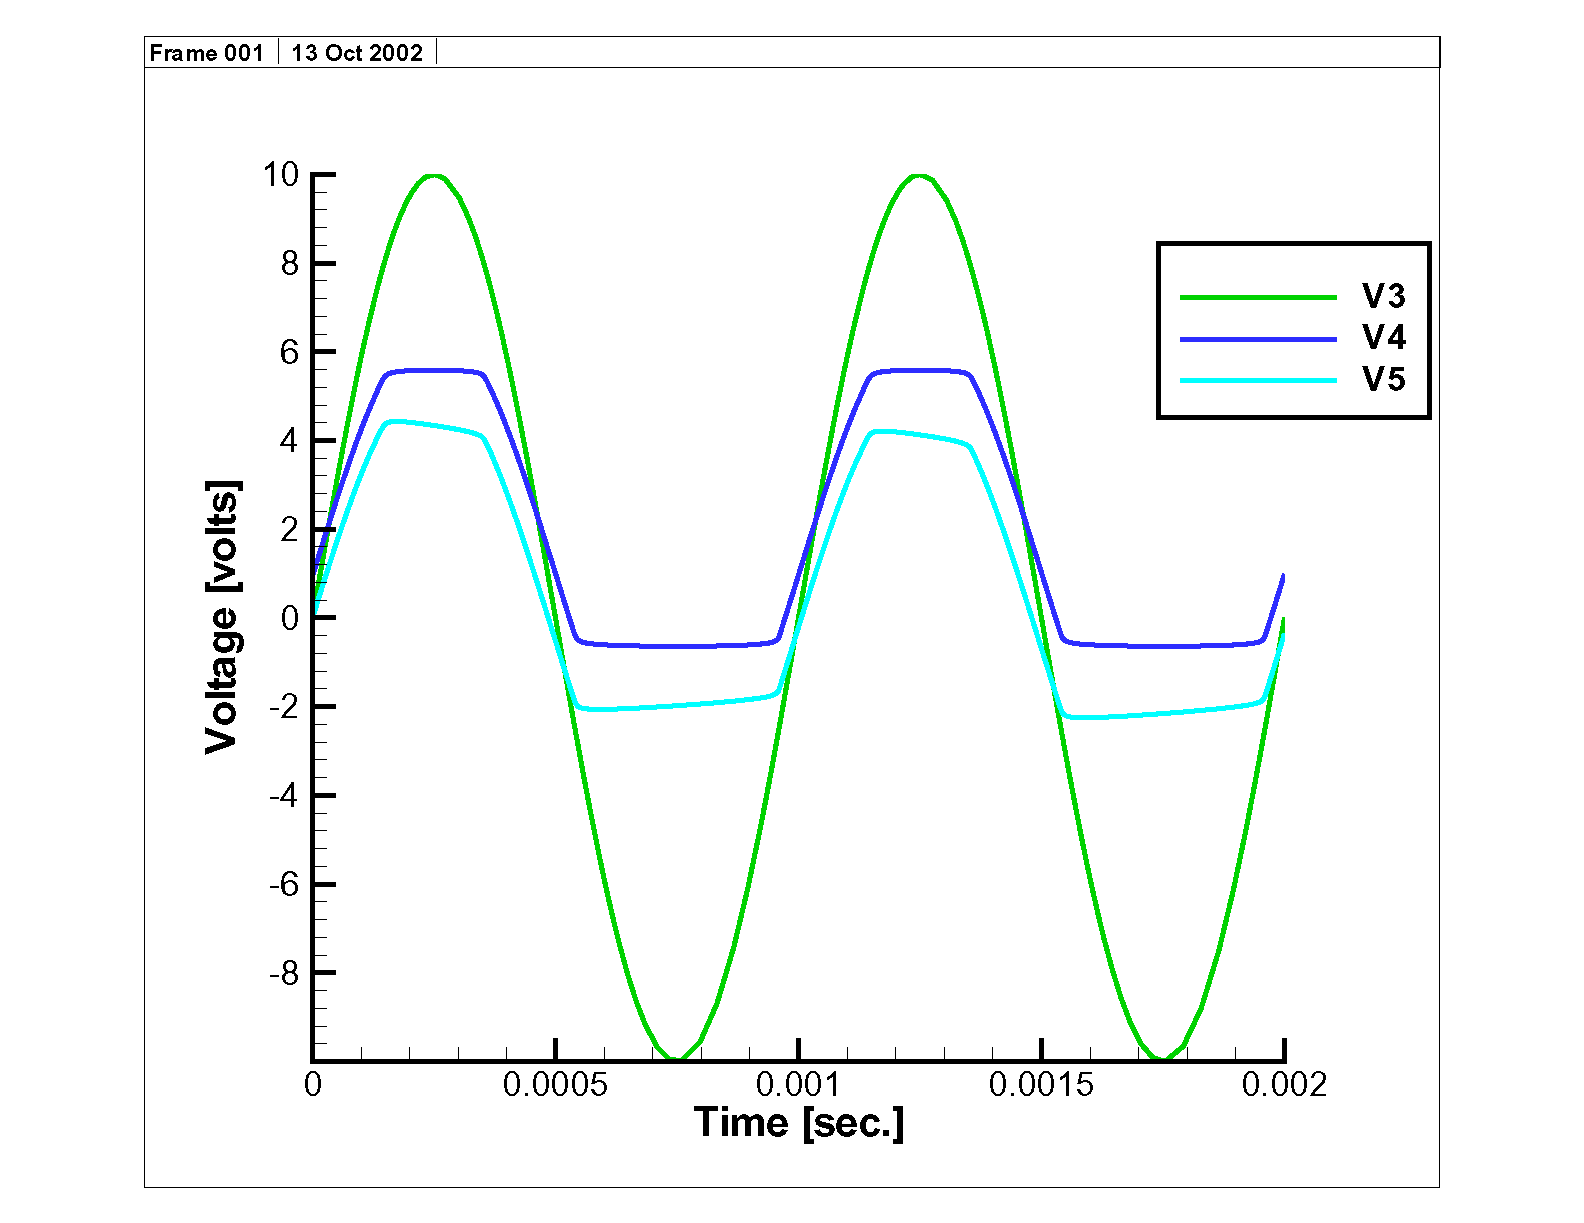
\includegraphics[width=4.5in]{clipper-tp}
      }
    \caption{TecPlot plot of diode clipper circuit transient response from \Xyce{}
      \texttt{.prn} file.\label{Clipper_TP}}
  \end{centering}
\end{figure}

%%% Local Variables:
%%% mode: latex
%%% End:

% END of Xyce_UG_ch12.tex ************

\cleardoublepage
% Sandia National Laboratories is a multimission laboratory managed and
% operated by National Technology & Engineering Solutions of Sandia, LLC, a
% wholly owned subsidiary of Honeywell International Inc., for the U.S.
% Department of Energy’s National Nuclear Security Administration under
% contract DE-NA0003525.

% Copyright 2002-2020 National Technology & Engineering Solutions of Sandia,
% LLC (NTESS).

%%-------------------------------------------------------------------------
%% Purpose        : Main LaTeX Xyce Users' Guide
%% Special Notes  : Graphic files (pdf format) work with pdflatex.  To use
%%                  LaTeX, we need to use postcript versions.  Not sure why.
%% Creator        : Robert Hoektra, Computational Sciences, SNL
%% Creation Date  : {12/22/2003}
%%
%%-------------------------------------------------------------------------

\chapter{Guidance for Running Xyce in Parallel}
\label{Parallel}
\index{\Xyce{}!running in parallel}

\chapteroverview{Chapter Overview}
{
This chapter provides guidance for running a parallel version of \Xyce{}, and includes the following sections:
\begin{XyceItemize}
\item Section~\ref{Parallel_Introduction}, {\em Introduction}
\item Section~\ref{paffinity}, {\em Processor Affinity on Linux systems}
\item Section~\ref{ProblemSize_Guidance}, {\em Problem Size}
\item Section~\ref{LinearSolver_Options}, {\em Linear Solver Options}
\item Section~\ref{Transformation_Options}, {\em Transformation Options}
\item Section~\ref{Device_Distribution_Options}, {\em Device Distribution Options}
\end{XyceItemize}
}

\section{Introduction}
\label{Parallel_Introduction}

\Xyce{} is designed from the ground up to be distributed-memory parallel, supported by the message-passing interface (MPI)
standard. Although many of the issues pertinent to running in parallel are still being researched, \Xyce{} is mature
enough that some general principles have emerged for efficiently running
problems in a parallel environment.  In addition to the information in this chapter, reference~\cite{xyceBookChapter:2011} provides
supplemental information about \Xyce{} parallel performance. 

Parallel simulations must be run from the command line.  Section~\ref{command_line_simulation} provides 
information about the parallel execution syntax for \Xyce{}.

\section{Processor Affinity on Linux systems}
\label{paffinity}

Beginning with release 1.8 of OpenMPI, the default behavior on Linux
systems is for OpenMPI to apply ``processor affinity'' to runs invoked
with mpirun.  This is intended to improve performance of parallel runs
by preventing the processes from moving around the system, possibly
degrading memory access efficiency.  Since most users of OpenMPI are
trying to maximize the performance of their systems, this is generally
a good change.

Prior to that release, the default behavior was to allow
MPI processes to be moved from processor to processor by the Linux
system as needed.

If you are the only person running MPI jobs on a system, and you are
only running one job, this change will have no impact on you, but if
you are running more than one MPI job at a time, or more than one user
on your system is running MPI jobs and the system is not using a
resource manager such as slurm, then this change has a profound impact
that must be understood and adapted to with mpirun options.

\subsection{Default OpenMPI Behavior with Processor Affinity Support}

At the time of this writing, OpenMPI's mpirun will, by default, bind
processes to a core if the number of processors requested is 2 or
less.  If the number of processes requested is greater than 2, it
will bind processes to a socket.

What this means is that once your run starts, each process of your
parallel job will be locked onto the processor (core or socket) on
which it started.

\subsection{Why You Have to Know About This}
Unfortunately, OpenMPI by default allocates processors to processes in
a round-robin fashion starting from the lowest numbered processor on
the system, and each mpirun makes this determination without any
access to what other mpirun invocations have done.

The effect of this is that if you start five identical 2-processor
parallel runs of \Xyce{} simultaneously on a 16-core system and don't add
extra mpirun options, each of these five jobs will be locked to the
\emph{same\/} two processors (processors 0 and 1) on the system.

{\bf Rather than getting five jobs run in the time it takes to run one,
each will only get 20\% of the two processors and take at least five
times longer to run than a single job would have.}

The same thing
would be true if five different users each ran one 2-processor \Xyce{}
job.  All jobs would be running on processors 0 and 1 of this
16-processor system.

Therefore, unless you are the only person on your system and you are
only running one job, you must be aware if OpenMPI is using processor
affinity on your system, and take appropriate steps to avoid
oversubscribing cores.

\subsection{Affected Systems}

At the time of this writing, OpenMPI supports processor affinity only
on Linux systems, and so the issues of this section apply only to
Linux.  The OS X kernel does not support jobs setting their own
processor affinity.  Some other systems have processor affinity
support in their kernels, but it is not yet supported by OpenMPI on
those systems.

Systems that are running a resource manager such as slurm (which
includes all of Sandia's high performance computing systems) are not
impacted by this issue, because slurm will allocate a specific set of
CPUs to be exclusive to your job, and no other jobs of yours or other
users can run on these CPUs.

\subsection{mpirun Command Line Options to Change Default Behavior}

If squeezing maximum performance out of the hardware is not important,
then the simplest way to avoid the oversubscription issue described
above is to use the \texttt{--bind-to none} option to mpirun.  This
was the default behavior of mpirun prior to release 1.8 of OpenMPI and
the default behavior of OpenMPI on every system other than Linux.
While the \texttt{--bind-to none} option will potentially allow your 
mpi processes to move around the
system and have degraded memory performance, it will \emph{NOT\/}
accidentally stack multiple jobs onto the same small set of
processors.  Any number of mpirun jobs may be run with this option,
and they will not compete for resources unless the Linux task
scheduler makes them do so.

If you do not want to do without the benefits that processor affinity
can bring, you can manually specify the set of CPUs that OpenMPI will
use for your job by using the \texttt{-cpu-set} option to mpirun,
chosing as your CPU set some numbered processors that you know are not
being used by other MPI jobs.  For example, \texttt{mpirun -np 2
  -cpu-set 2-3} will run your 2 processor job with the jobs locked to
processors 2 and 3 instead of to processors 0 and 1.  You will have to
make sure to use a different CPU set for each job, and make sure that
you are not using the same CPU set as some other user on the system.

There are other options for modifying OpenMPI's processor binding
behavior, so consult OpenMPI documentation if you wish to understand
them better.

Finally, if you really want to solve the problem correctly, reaping
both the benefits of processor affinity and the simplicity of using
mpirun's defaults, you can install and configure a resource manager on
your system.  This is a topic that is far outside the scope of \Xyce{}
documentation.  See \url{http://slurm.schedmd.com/} for documentation
on one such resource manager.


\section{Problem Size}
\label{ProblemSize_Guidance}

Running \Xyce{} in parallel is often useful for circuits with thousands of devices or more.  However, due to the overhead of interprocessor communication,
 there is an optimal number of processors that will achieve the best performance.  This number is dependent upon many factors, including the number and 
type of devices, the topology of the circuit, and the characteristics of the computing architecture.  It is difficult to know a priori what this optimal 
number of processors is.  However, it is apparent when that optimal number is exceeded because, as the number of processors is increased, 
the total simulation time will also increase.  This is due to the increasing amount of required communication and decreasing amount of work per processor.
In other words, the benefit of distributing the problem is outweighed by the communication overhead, so increasing the processor count beyond this
optimal point is counterproductive.

\subsection{Ideal Problem Size}
In general, a circuit needs to be relatively large to take full advantage of the parallel capability of \Xyce{}. 
However, parallelism is achieved in two distinct phases of the code:  the device evaluation and the linear solve.
The device evaluation is, as the name implies, the evaluation of all the device equations in order to compute the residual vector 
and Jacobian entries for Newton's method.  \Xyce{} distributes the number of devices over the number of processors in parallel, 
so their evaluation enables speedups in the total simulation time even for thousands of devices. 

The linear solve phase is more computationally complex.  The Jacobian matrix generated by most circuits is sparse and has heterogeneous structure, in 
that there is not a regular sparsity pattern in the matrix nonzeros.  Sparse, direct linear solvers have proven to be efficient on these types of 
linear systems up into the tens to hundreds of thousands of unknowns.  They become less efficient for linear systems in the hundreds of thousands of unknowns.  
This is where iterative linear solvers can provide scalable performance because of their inherent parallelism.  Unfortunately, the effectiveness of 
iterative linear solvers is dependent upon preconditioning the linear system (see Section~\ref{Preconditioning_Options}).  
The benefit of direct over iterative linear solvers is that they rarely fail to compute a solution, so direct
linear solvers are the more robust option for enabling simulations to complete.  

In general, there are three modes in which \Xyce{} can
be executed:  ``Serial load, serial solve'', ``Parallel load, serial solve'', and ``Parallel load, parallel solve''.  
Each of these modes optimizes the amount of available parallelism for a given linear system size, as summarized in Table~\ref{tab:sim:modes}.  The ``load'' refers to the device evaluation phase combined with the assembly of the Jacobian matrix and residual vector, while
the ``solve'' refers to the linear solve phase. 
``Serial load, serial solve'' is the only mode of computation that a serial version of \Xyce{} will perform, but it can also be
obtained in a parallel version of \Xyce{} by using only one MPI processor.  Both of the ``Parallel load'' simulation modes require a parallel build of \Xyce{}, where the linear solver method can be a direct method (``serial solve'') or an iterative method (``parallel solve'') using
the options discussed in Section~\ref{LinearSolver_Options}.
Hybrid linear solvers, which combine the best attributes of both direct and iterative methods, provide a robust and scalable option. 
They are not reflected in Table~\ref{tab:sim:modes}, but more information about these types of linear solvers will be discussed in 
Section~\ref{HybridLinearSolver_Options}.  

\begin{table}[htp]
\caption[\Xyce{} Simulation Modes]{Xyce simulation modes.}
\label{tab:sim:modes}
\begin{center}
\begin{tabular}{| p{5cm} | p{3.5cm} | p{7cm} |}
\hline
Mode & Linear System Size & Reason \\
\hline
``Serial load, serial solve'' & $10^0$ - $10^3$ & MPI overhead cannot speed up device evaluation or linear solve. \\
``Parallel load, serial solve'' & $10^3$ - $10^5$ & Distributed device evaluations can speed up the simulation, but 
iterative linear solvers are not more efficient than direct methods.\\
``Parallel load, parallel solve'' & $10^5$ or more & Distributed device evaluations can speed up the simulation and
so can iterative linear solvers, if an efficient preconditioner is available. \\
\hline
\end{tabular}
\end{center}
\end{table}

\subsection{Smallest Possible Problem Size}
Circuits consist of a discrete set of components (voltage nodes, devices, etc.). For parallel simulation, it is preferable that \Xyce{} be able to put 
at least one discrete component of the problem on each processor. In practice, this means the circuit should be distributed across fewer processors than 
the number of nodes and devices it contains.

\section{Linear Solver Options}
\label{LinearSolver_Options}

The different linear solvers available in \Xyce{} are:

\begin{XyceItemize}
  \item KLU
  \item KSparse
  \item SuperLU and SuperLU DIST (optional)
  \item The AztecOO iterative solver library
  \item The Belos iterative solver library
  \item The ShyLU hybrid solver library (optional)
\end{XyceItemize}

AztecOO and Belos are the parallel iterative solvers and KLU, KSparse, and SuperLU (optional)
are the serial direct solvers that are available for both serial and parallel builds of \Xyce{}.  
If KLU, KSparse, or SuperLU is used with a parallel version of \Xyce{}, the devices are evaluated and
linear problem is assembled in parallel, but the linear system is solved in serial
on one processor.  This can be quite effective for circuits with tens of thousands of devices
or fewer (see Table~\ref{tab:sim:modes}). The ShyLU hybrid linear solver, which combines the robustness
of a direct solver with the scalability of an iterative solver, will be discussed in 
Section~\ref{HybridLinearSolver_Options}.  

The user can specify the solver through the \texttt{.OPTIONS LINSOL} control line 
in the netlist.  The default linear solver used by \Xyce{} is described in Table~\ref{tab:default:solver}.
By default, a parallel version of \Xyce{} uses AztecOO as the linear solver when the linear
system is larger than ten thousand unknowns.  For any linear system smaller than ten thousand unknowns,
\Xyce{} uses KLU as the linear solver.  A serial version of \Xyce{} uses KLU as its default linear 
solver.  To use a solver other than the default the user needs to add the option 
``\texttt{TYPE=<solver>}'' to the \texttt{.OPTIONS LINSOL}
control line in the netlist, where \texttt{<solver>}
is `\texttt{KLU},' `\texttt{KSPARSE},' `\texttt{SUPERLU},' `\texttt{SUPERLUDIST},' `\texttt{AZTECOO},' `\texttt{BELOS},' or `\texttt{SHYLU}.'

\begin{table}[htp]
\caption[\Xyce{} Default Linear Solver]{Xyce default linear solver.}
\label{tab:default:solver}
\begin{center}
\begin{tabular}{| p{3cm} | p{3cm} | p{4cm} |}
\hline
Solver & Version & Linear System Size\\
\hline
KLU & Serial & {\it all} \\
KLU & Parallel & $1-(10^5-1)$ unknowns \\
AztecOO & Parallel & $10^5+$ unknowns \\
\hline
\end{tabular}
\end{center}
\end{table}

\subsection{KLU}
KLU is a serial, sparse direct solver native to the Amesos package in Trilinos~\cite{trilinos:toms} and is the default solver for serial builds of \Xyce{}. 
KLU is the default solver for small circuits in parallel builds of \Xyce{} as well, but this requires the linear system to be solved 
on one processor and the solution communicated back to all processors. As long as the linear system can fit on one processor, KLU is 
often a superior approach to using an iterative linear solver.  So, if a parallel build of \Xyce{} is run in serial on a circuit that generates a linear system
larger than one thousand unknowns and the simulation fails to converge, then specifying KLU as the linear solver may fix that problem.  

Some of the solver parameters for KLU can be altered through the `\texttt{.OPTIONS LINSOL}' control line in the netlist.  
Table \ref{tab:klu:options} lists solver parameters and their default values for KLU.
   
\begin{table}[htp]
\caption[ KLU linear solver options.] {KLU linear solver options.}
\label{tab:klu:options}
\begin{center}
\begin{tabular}{| p{3.5cm} | p{9cm} | p{2.5cm} |}
\hline
Option & Description & Default Value \\
\hline
{\tt KLU\_repivot}         & Recompute pivot order each solve & 1 (true) \\
{\tt output\_ls}           & Write out linear systems solved by KLU to file every \# solves & 0 (no output)\\
{\tt output\_base\_ls}     & Write out linear systems before any transformations to file every \# solves & 0 (no output)\\
{\tt output\_failed\_ls}   & Write out linear systems KLU failed to solve to file & 0 (no output) \\
\hline
\end{tabular}
\end{center}
\end{table}

\subsection{KSparse}
KSparse is a serial, sparse direct solver based on Ken Kundert's sparse solver, Sparse 1.3.  Kundert's sparse solver was developed 
as part of the SPICE circuit simulation code.  KSparse is built, by default, in \Xyce{}.  Similar to KLU,
KSparse can be used in a parallel version of \Xyce{}, but the linear system is solved on one processor.

\subsection{SuperLU and SuperLU DIST}
SuperLU is a serial, sparse direct solver and SuperLU DIST is a parallel, sparse direct solver with an interface in the 
Amesos package.  SuperLU and SuperLU DIST support are {\it optionally} built in \Xyce{},
so they are not available by default in any \Xyce{} build or provided binary.  Furthermore, to enable SuperLU and 
SuperLU DIST support in \Xyce{}, it is necessary to build SuperLU and SuperLU DIST support in Amesos/Trilinos.  Similar to KLU, 
SuperLU can be used in a parallel version of \Xyce{}, but the linear system is 
solved on one processor.  SuperLU DIST can only be used in a parallel version of \Xyce{}, the Amesos interface handles the redistribution
of the matrix into the format required by SuperLU DIST.  
\Xyce{} does not allow modifications to SuperLU and SuperLU DIST solver parameters. 


\subsection{AztecOO}
AztecOO is a package in Trilinos~\cite{trilinos:toms} that offers an assortment of iterative linear solver algorithms.  
\Xyce{} uses the Generalized Minimal Residual (GMRES) method~\cite{sasc86} from this suite of iterative solvers.  
Some of the solver parameters for GMRES can be altered through the `\texttt{.OPTIONS LINSOL}' control line in the netlist. 
Table~\ref{tab:aztecoo:options} provides a list of solver parameters for AztecOO and their default values.

\begin{table}[htp]
\caption[AztecOO linear solver options.]{AztecOO linear solver options.}
\label{tab:aztecoo:options}
\begin{center}
\begin{tabular}{| p{3cm} | p{9cm} | p{2.5cm} |}
\hline
Option & Description & Default Value \\
\hline
{\tt AZ\_max\_iter}        & Maximum allowed iterations & 200 \\
{\tt AZ\_tol}              & Iterative solver (relative residual) tolerance & 1.0e-9 \\
{\tt AZ\_kspace}           & Krylov subspace size & 50 \\
{\tt output\_ls}           & Write out linear systems solved by AztecOO to file every \# solves & 0 (no output)\\
{\tt output\_base\_ls}     & Write out linear systems before any transformations to file every \# solves & 0 (no output)\\
\hline
\end{tabular}
\end{center}
\end{table}

\subsubsection{Common AztecOO Warnings}

If \Xyce{} is built with the verbosity enabled for the linear algebra package, it is not
uncommon to see warnings from AztecOO usually indicating the solver returned unconverged due to a numerical issue.

\begin{center}
\begin{minipage}{0.85\textwidth}
\color{XyceRed} {\bf NOTE:  }\color{black}  AztecOO warnings {\em do not} indicate the entire simulation has failed, \Xyce{} uses a hierarchy of solvers so if the iterative linear solver fails, the nonlinear solver or time integrator will usually make adjustments and attempt the step again; so the warnings can often be ignored. If the entire simulation eventually fails (i.e., gets a ``time-step-too-small'' error), then the AztecOO warnings might contain clues as to what went wrong.
\end{minipage}
\end{center}

The simplest reason for AztecOO to return unconverged would be when the maximum number of 
iterations is reached, resulting in the following warning:
\begin{verbatim}
***************************************************************
Warning: maximum number of iterations exceeded without convergence
***************************************************************
\end{verbatim}
Another reason AztecOO may return unconverged is when the GMRES Hessenberg
matrix is ill-conditioned, which is usually a sign that the matrix and/or
preconditioner is nearly singular, resulting in the following warning:
\begin{verbatim}
***************************************************************
Warning: the GMRES Hessenberg matrix is ill-conditioned.  This may
indicate that the application matrix is singular. In this case, GMRES
may have a least-squares solution.
***************************************************************
\end{verbatim}
It is also common to lose accuracy when either the matrix or preconditioner, or both,
are nearly singular.  GMRES relies on an estimate of the residual norm,
called the recursive residual, to determine convergence.  \Xyce{} uses the recursive
residual instead of the actual residual for computational efficiency.
However, numerical issues can cause the recursive residual to differ
from the actual residual.  When AztecOO detects but
cannot rectify this situation, it outputs the following warning:
\begin{verbatim}
***************************************************************
Warning: recursive residual indicates convergence
though the true residual is too large.

Sometimes this occurs when storage is overwritten (e.g. the
solution vector was not dimensioned large enough to hold
external variables). Other times, this is due to roundoff. In
this case, the solution has either converged to the accuracy
of the machine or intermediate roundoff errors occurred
preventing full convergence. In the latter case, try solving
again using the new solution as an initial guess.
***************************************************************
\end{verbatim}

\subsection{Belos}
\label{Belos_Options}
Belos is a package in Trilinos~\cite{trilinos:toms} that offers an assortment of iterative linear
solver algorithms.  Many of the algorithms available in Belos can also be found in AztecOO.  However, Belos
offers a few computational advantages because its solvers are implemented using templated C++.  
In particular, AztecOO can solve linear systems only in double-precision arithmetic, while Belos
can solve linear systems that are complex-valued or in extended-precision arithmetic.  At this time,
\Xyce{} is using a subset of Belos capabilities, the default method is GMRES, and the 
interface to Belos will recognize most of the AztecOO linear solver options, as shown in 
Table~\ref{tab:belos:options}.

\begin{table}[htp]
\caption[Belos linear solver options.]{Belos linear solver options.}
\label{tab:belos:options}
\begin{center}
\begin{tabular}{| p{3cm} | p{9cm} | p{2.5cm} |}
\hline
Option & Description & Default Value \\
\hline
{\tt AZ\_max\_iter}        & Maximum allowed iterations & 200 \\
{\tt AZ\_tol}              & Iterative solver (relative residual) tolerance & 1.0e-9 \\
{\tt AZ\_kspace}           & Krylov subspace size & 50 \\
{\tt output\_ls}           & Write out linear systems solved by Belos to file every \# solves & 0 (no output)\\
{\tt output\_base\_ls}     & Write out linear systems before any transformations to file every \# solves & 0 (no output)\\
\hline
\end{tabular}
\end{center}
\end{table}

\subsection{Preconditioning Options}
\label{Preconditioning_Options}

Iterative linear solvers often require the assistance of a preconditioner
to efficiently compute a solution of the linear system
\begin{equation}
\label{axb}
Ax=b
\end{equation}
\noindent to the requested accuracy.  
A preconditioner, $M$, is an approximation to the original matrix $A$ that is inexpensive
to solve.  Then (\ref{axb}) can be rewritten to include this (right) preconditioner as
\begin{equation}
\label{axb:prec}
AM^{-1}y=b,
\end{equation}
\noindent where $x=M^{-1}y$ is the solution to the original linear system.
If $M=A$, then the solution to the linear system is found in one iteration.
In practice, $M$ is a good approximation to $A$, then it will take few iterations
to compute the solution of the linear system to the requested accuracy.
By default, \Xyce{} uses a non-overlapped additive Schwarz preconditioner with 
an incomplete LU factorization on each subdomain~\cite{Saad:2003:IMSLS}.  
The parameters of the incomplete LU factorization are found in Table~\ref{tab:prec_options}.  
This is a simple preconditioner that always works, but is not always the most effective, 
so other preconditioning options will be presented in this section.    

\Xyce{} provides access to preconditioning packages in Trilinos~\cite{trilinos:toms}, 
such as Ifpack, through an expanded preconditioning interface.  
If modifications to the preconditioner are necessary, the user may specify the preconditioner 
through the `\texttt{.OPTIONS LINSOL}' control line in the netlist. 
Table \ref{tab:prec_options} provides a list of preconditioner parameters and
their default values.  

\begin{table}[htp]
\caption[Preconditioner options.]{Preconditioner options.}
\label{tab:prec_options}
\begin{center}
\begin{tabular}{| p{3.5cm} | p{8cm} | p{2.5cm} |}
\hline
Option & Description & Default Value \\
\hline
{\tt prec\_type}           & Preconditioner & Ifpack \\
{\tt AZ\_ilut\_fill}       & ILU fill level & 2.0 \\
{\tt AZ\_drop}             & ILU drop tolerance & 1.0e-3 \\
{\tt AZ\_overlap}          & ILU subdomain overlap & 0 \\
{\tt AZ\_athresh}          & ILU absolute threshold & 0.0001 \\
{\tt AZ\_rthresh}          & ILU relative threshold & 1.0001 \\
{\tt use\_aztec\_precond}  & Use native ILU from AztecOO package & 0 (false) \\
{\tt use\_ifpack\_factory} & Use Ifpack factory to create preconditioner & 0 (false) \\
{\tt ifpack\_type}         & Control which preconditioner Ifpack factory creates (ILU, ILUT, Amesos) & Amesos \\
\hline
\end{tabular}
\end{center}
\end{table}

In practice, the choice of an effective preconditioner is highly problem dependent.  By default,
\Xyce{} provides a preconditioner that works for most circuits, but is not the best preconditioner
for all circuits.  One simple modification to the default preconditioner that often makes it more
effective is the use of a sparse direct solver on each subdomain, instead of an inexact factorization: \\[0.5em] 
\noindent \verb|.OPTIONS LINSOL USE_IFPACK_FACTORY=1| \\[0.5em]
This preconditioner will fail if there is a singular subdomain matrix because the KLU solver on that subdomain will fail.
If numerical difficulties are not encountered during the simulation, this preconditioner is superior to inexact factorizations.
A more advanced preconditioner that has been effective for certain types of circuits uses the block triangular form (BTF)
permutation of the original matrix before generating the additive Schwarz preconditioner.  This preconditioner, which
is published in ~\cite{ICCAD09_precond}, will be presented in Section~\ref{BTF_Precond}.


\subsection{ShyLU}
\label{HybridLinearSolver_Options}
ShyLU is a package in Trilinos~\cite{trilinos:toms} that provides a hybrid linear solver 
designed to be a black-box algebraic solver~\cite{ShyLU-IPDPS}. 
ShyLU support is {\it optionally} built in \Xyce{},
so it is not available by default in any \Xyce{} build or provided binary.
Furthermore, to enable ShyLU support in \Xyce{}, it is necessary to build 
the ShyLU package in Trilinos.

ShyLU is hybrid in both the
parallel programming sense - using MPI and threads - and in the mathematical
sense - using features from direct and iterative methods. \Xyce{} uses ShyLU as a global
Schur complement solver~\cite{Saad:2003:IMSLS}.  This solver can be expensive, but also
has proven to be a robust and scalable approach for some circuit matrices~\cite{bomhof00}. 

ShyLU is under active development and testing in \Xyce{}, so a minimum number of options are 
provided to the user for controlling this solver.  The solution approach is static, 
the diagonal blocks of the partitioned matrix are solved using KLU, while the Schur complement 
is solved using an iterative method (AztecOO's GMRES specifically). 
The matrix partitioning is generated using a wide separator, which is a conventional 
vertex separator where all the vertices that are adjacent to the separator in one of the subgraphs
are added in.  The only options that can be modified are shown
in Table~\ref{tab:shylu:options}.  This includes the maximum number of iterations and solver tolerance
used by GMRES and the dropping threshold that ShyLU uses to generate a preconditioner for GMRES.

\begin{table}[htp]
\caption[ShyLU linear solver options.]{ShyLU linear solver options.}
\label{tab:shylu:options}
\begin{center}
\begin{tabular}{| p{3cm} | p{9cm} | p{2.5cm} |}
\hline
Option & Description & Default Value \\
\hline
{\tt AZ\_max\_iter}        & Maximum allowed iterations & 30 \\
{\tt AZ\_tol}              & Iterative solver (relative residual) tolerance & 1.0e-12 \\
{\tt ShyLU\_rthresh}       & Relative dropping threshold for Schur complement preconditioner & 1.0e-3 \\ 
{\tt output\_ls}           & Write out linear systems solved by ShyLU to file every \# solves & 0 (no output)\\
{\tt output\_base\_ls}     & Write out linear systems before any transformations to file every \# solves & 0 (no output)\\
\hline
\end{tabular}
\end{center}
\end{table}



\section{Transformation Options}
\label{Transformation_Options}

Transformations are often used to permute the original linear system to one that
is easier or more efficient for direct or iterative linear solvers.  \Xyce{} has many different permutations 
that can be applied to remove dense rows and columns from a matrix, reduce fill-in, find a block triangular form, 
or partition the linear system for improved parallel performance. 

\subsection{Removing Dense Rows and Columns}
The transformation that reduces the linear system through removal of all rows and 
columns with single non-zero entries in the matrix is called singleton filtering.  The values
associated with these removed entries can be resolved in a pre- or post-processing
phase with the linear solve.
A by-product of this transformation is a more tractable and sparse 
linear system for the load balancing and linear solver
algorithms.  This functionality can be turned on by adding 
`\texttt{TR\_SINGLETON\_FILTER=1}' to the `\texttt{.OPTIONS LINSOL}'
control line in the netlist.  This option is enabled by default whenever iterative
solvers are used in \Xyce{}.

\subsection{Reordering the Linear System}
Approximate Minimum Degree (AMD) ordering is a symmetric permutation that 
reduces the fill-in for direct factorizations.  If given a nonsymmetric
matrix $A$, the transformation computes the AMD ordering of $A + A^T$.  
This functionality may be turned on by adding `\texttt{TR\_AMD=1}' 
to the `\texttt{.OPTIONS LINSOL}' control line in the netlist. 
For parallel builds of \Xyce{}, AMD ordering is enabled by default whenever iterative solvers
are used.  In parallel, the AMD ordering is performed only on the local graph for
each processor, not the global graph.  This is to reduce the fill-in for the incomplete
LU factorization used by the additive Schwarz preconditioner, see Section~\ref{Preconditioning_Options}.

\subsection{Partitioning the Linear System}
\label{Partitioning_Linear_System}

Partitioning subdivides the linear system and 
then distributes it to the available processors.  A good partition can have a dramatic 
effect on the parallel performance of a circuit simulation tool.  
There are two key components to a good partition:

\begin{XyceItemize}
  \item Effective load balance\index{parallel!load balance}
  \item Minimizing communication\index{parallel!communication} overhead.  
\end{XyceItemize}

An effective load balance ensures the computational load of the calculation is equally distributed among 
available processors. Minimizing communication overhead seeks to distribute the problem in a way to reduce 
impacts of underlying message passing during the simulation run. For runs with a small number of devices 
per processor the communication overhead becomes the critical issue, while for runs with larger numbers 
of devices per processor the load balancing becomes more important.  

\Xyce{} provides hypergraph partitioning via the \textbf{Zoltan}\index{ZOLTAN} library of parallel 
partitioning heuristics integrated into \Xyce{}.  The Isorropia package in Trilinos provides access to \textbf{Zoltan}\index{ZOLTAN} and 
can be controlled through the `\texttt{.OPTIONS LINSOL}'\index{\texttt{.OPTIONS}!\texttt{LINSOL}} 
control line in the netlist. Table \ref{tab:partitioning:options} provides
the partitioning options and their default parameters. For parallel builds of 
\Xyce{}, when iterative solvers are used, \textbf{Isorropia} is enabled by default to use hypergraph partitioning. 
The linear system is statically load balanced at the beginning of the simulation based 
on the graph of the Jacobian matrix.  

\begin{table}[htp]
\caption[Partitioning options.]{Partitioning options.}
\label{tab:partitioning:options}
\begin{center}
\begin{tabular}{| p{3.5cm} | p{6cm} | p{4.5cm} |}
\hline
Option & Description & Default Value \\
\hline
{\tt TR\_PARTITION}        & Partitioning package & 0 (none), serial, \\
                           &                      & 1 (Isorropia), parallel \\
{\tt TR\_PARTITION\_TYPE}  & Isorropia partitioner type & \verb|HYPERGRAPH| \\
\hline
\end{tabular}
\end{center}
\end{table}

\Xyce{} includes an expanded partitioning interface to allow the user to access multiple partitioners through Isorropia. 
Users may change the partitioner provided by adding `\texttt{TR\_PARTITION\_TYPE}' to the `\texttt{.OPTIONS LINSOL}' control line in
the netlist. There are two options for partitioning:  hypergraph
(`\texttt{TR\_PARTITION\_TYPE=HYPERGRAPH}') and, optionally, graph (`\texttt{TR\_PARTITION\_TYPE=GRAPH}') partitioning through ParMETIS.
Occasionally it is desirable to turn off the partitioning option, even for parallel simulations.   To do so, users can add the 
`\texttt{TR\_PARTITION=0}' to the `\texttt{.OPTIONS LINSOL}' control line.

These techniques can be very effective for improving the
efficiency of the iterative linear solvers\index{solvers!iterative linear}.
See the \textbf{Zoltan User Guide}~\cite{zoltan:user} for more details.

\subsection{Permuting the Linear System to Block Triangular Form}
\label{BTF_Precond}
The block triangular form (BTF) permutation is often useful for direct and iterative
solvers, enabling a more efficient computation of the linear system solution.
In particular, the BTF permutation has shown promise when it is combined with
an additive Schwarz preconditioner (see Section~\ref{Preconditioning_Options}) in the simulation of
circuits with unidirectional flow.  

The global BTF transformation computes the permutation of the linear system to
block triangular form, and uses the block structure to partition the linear system. The partitioning can be
a simple linear distribution of block rows, `\texttt{TR\_GLOBAL\_BTF=1}', or a
hypergraph partitioning of block rows, `\texttt{TR\_GLOBAL\_BTF=2}.'
As the global BTF transformation includes elements of other tranformations,
it is imperative to turn off other linear solver options.  
To use the global BTF, the linear solver control line in the netlist should 
contain: \\[0.5em] 
\noindent \verb|.OPTIONS LINSOL TR_GLOBAL_BTF=<1,2> TR_SINGLETON_FILTER=1|\\
\noindent \verb|+ TR_AMD=0 TR_PARTITION=0|

This transformation is only useful in parallel when using a preconditioned iterative solver.
It is often more effective when combined with the exact factorization of each subdomain,
given by the `\texttt{USE\_IFPACK\_FACTORY=1}' option.  In practice, the structure
that this transformation takes advantage of is found in CMOS memory circuits~\cite{ICCAD09_precond}.


\section{Device Distribution Options}
\label{Device_Distribution_Options} 
\Xyce{} uses different parallel distributions for the objects that evaluate the
device models and the linear system.  As discussed in Section~\ref{Partitioning_Linear_System}, a good
parallel partition of the linear system can improve load balance and minimize communication. 
The same is true for the parallel distribution of devices, since they have widely varying
computational cost and the circuit connectivity graph is often irregular.  Furthermore, a more efficient
device distribution strategy can overlap netlist processing with the simulation setup, enabling scalable
parsing for larger netlists.

\begin{table}[htp]
\caption[Device Distribution options.]{Distribution options.}
\label{tab:distribution:options}
\begin{center}
\begin{tabular}{| p{3.5cm} | p{6cm} | p{4.5cm} |}
\hline
Option & Description & Default Value \\
\hline
{\tt STRATEGY}        & Distribution strategy & 0 \\
\hline
\end{tabular}
\end{center}
\end{table}

\Xyce{} provides three different device distribution strategies that can be controlled through
the \texttt{.OPTIONS DIST}\index{\texttt{.OPTIONS}!\texttt{DIST}} control line in the netlist,
see Table \ref{tab:distribution:options}.  The default strategy (\texttt{STRATEGY=0}) that \Xyce{} 
uses for parallel device distribution is a first-come-first-served
approach, in that the total number of devices in a circuit is divided evenly over the number
of parallel processors in the order of parsing.  This is the simplest distribution strategy, but
it does not take into account the connectivity of a circuit or balance device model computation.
Therefore, this strategy can exhibit parallel imbalance for post-layout circuits that have a 
substantial portion of parasitic devices.

\Xyce{} provides two other distribution strategies that enable scalable parsing for
flattened circuits or distribute devices in a more balanced manner.  The "flat round robin" strategy
(\texttt{STRATEGY=1}) will generate the same device distribution as the default strategy, but every
parallel processor will participate in reading their portion of the netlist.  In that way, this
strategy provides a more scalable setup than the default strategy, but can only be applied to flattened
(non-hierarchical) netlists.  The "device balanced" strategy (\texttt{STRATEGY=2}) will evenly divide
each of the device types over the number of parallel processors, so each processor will have a balanced
number of each model type.  This allieviates the parallel imbalance in the device model computation that
can be experienced with post-layout circuits.  However, it does not take into account the circuit
connectivity, so the communication will not be minimized by this strategy.




%%% Local Variables:
%%% mode: latex
%%% End:

%% END of Xyce_UG_ch13.tex ************

\cleardoublepage
% Sandia National Laboratories is a multimission laboratory managed and
% operated by National Technology & Engineering Solutions of Sandia, LLC, a
% wholly owned subsidiary of Honeywell International Inc., for the U.S.
% Department of Energy’s National Nuclear Security Administration under
% contract DE-NA0003525.

% Copyright 2002-2020 National Technology & Engineering Solutions of Sandia,
% LLC (NTESS).

%%-------------------------------------------------------------------------
%% Purpose        : Main LaTeX Xyce Users' Guide
%% Special Notes  : Graphic files (pdf format) work with pdflatex.  To use
%%                  LaTeX, we need to use postcript versions.  Not sure why.
%% Creator        : Scott A. Hutchinson, Computational Sciences, SNL
%% Creation Date  : {05/23/2002}
%%
%%-------------------------------------------------------------------------

% -------------------------------------------------------------------------
% two level Analysis Chapter ----------------------------------------------
% -------------------------------------------------------------------------

\chapter{Handling Power Node Parasitics}
\label{PowerNode_Chap}
\index{two-level Newton}
\index{power node parasitics}

\chapteroverview{Chapter Overview}
{
This chapter includes the following sections:
\begin{XyceItemize}
\item Section~\ref{powerNode_Overview}, {\em Power Node Parasitics}
\item Section~\ref{twolevel_Overview}, {\em Two Level Algorithms Overview}
\item Section~\ref{twolevel_Examples}, {\em Examples}
\item Section~\ref{twolevel_restart}, {\em Restart}
\end{XyceItemize}
}

\section{Power Node Parasitics}
\label{powerNode_Overview}
\index{power node parasitics}

Parasitic elements (R, L, C) are frequently required for circuit simulations
to capture important circuit behavior.  Most parasitic elements 
(interconnects, etc.) can be added to netlists without causing any 
difficulties for the \Xyce{} solvers.   Small circuits in particular are
very robust to the addition of parasitic elements. Larger circuits, however, 
that must be simulated in parallel will in general tend to 
have more solver difficulties with the addition of parasitic devices.  
Of particular note are parasitic elements attached to the power and/or
ground nodes of large digital circuits.  An example of this is shown in
figure~\ref{powerNodeExample}.  As these nodes tend to be highly 
connected, they can potentially have a very high impact on solver difficulties.  

%  power node figure
\begin{figure}[b]
\vspace{-5pt}
  \centering
  \scalebox{0.40}
    {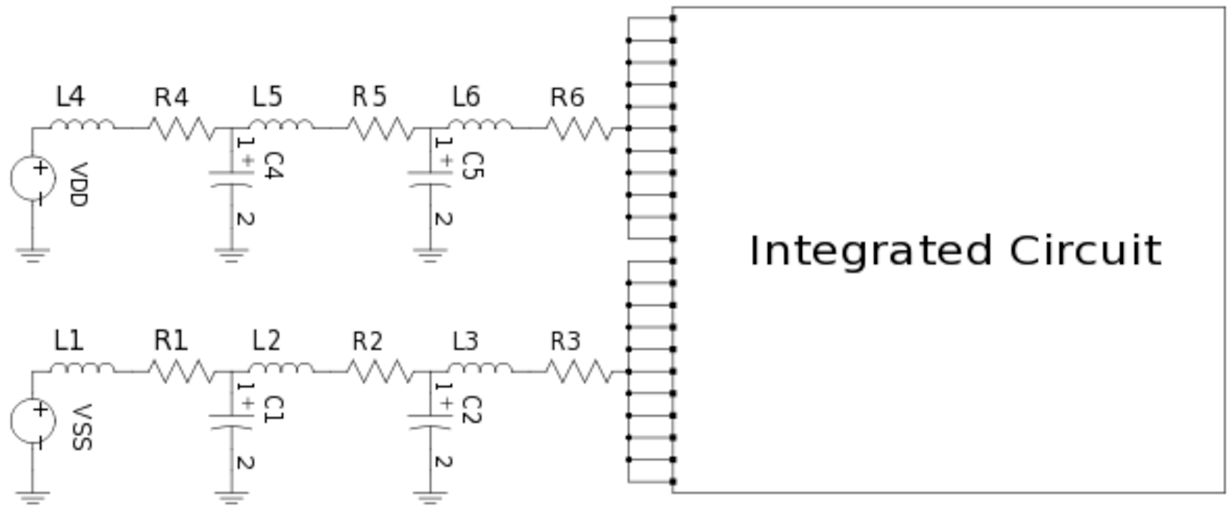
\includegraphics{paras_networkv2.pdf}}
\vspace{-5pt}
    \caption[Power node parasitics example.] {Power node parasitics example. 
NOTE:	An RLC network sits between the VDD, VSS sources and the main circuit, so these highly connected nodes cannot be removed with a singleton filter.}
    \label{powerNodeExample}
  \vspace{-10pt}
\end{figure}


One of the parallel algorithms used by \Xyce{} is called \emph{singleton 
removal}~\cite{ICCAD09_precond}, which is applied at the linear solver level and is crucial for getting many large circuits to run in parallel. This algorithm takes advantage of the fact that, in circuit simulation, some solution values are available explicitly, rather than being a quantity that needs to be calculated as the solution to a particular equation. In circuit simulation, such quantities are usually the values of independent sources. For instance, the presence of an independent voltage source at a particular node in a circuit fixes the voltage at that node to be the value of the independent source; therefore, equations reflecting the value of the voltage at that particular node do not have to be added to the set of linear equations used (in part) to determine the voltages at all the nodes in the circuit. The technique of fixing such node voltages without including them in the rest of the linear solve can be handled in a preprocessing phase referred to as the singleton removal phase.  

When simulating in parallel, singleton removal is crucial as some voltage 
sources (especially power supplies in digital circuits) are connected to 
hundreds or thousands of circuit nodes.  This presents a big 
problem in parallel because having numerous connections can often mean a communication 
bottleneck during the linear solve. Using singleton removal eliminates 
that bottleneck.

While singleton removal can result in a great improvement for circuits with 
ideal power supplies, for circuits with nonideal power supplies, the 
communication bottleneck remains.   Once parasitic elements 
are placed between the power supply and the rest of the circuit, it is only 
the voltage at the circuit node directly connected to the independent
source that can be removed via singleton removal.  Other nodes connected to this independent source through parasitic elements have 
voltages that must now be solved for directly.  


\section{Two Level Algorithms Overview}
\label{twolevel_Overview}

Fortunately, \Xyce{}~\cite{xyceBookChapter:2011} provides a workaround 
that allows power node parasitics to be included in large circuits without breaking singleton 
removal.  The workaround requires the use of a two-level Newton solve,
in which the problem is divided into two very separate pieces, each
for the most part treated as an entirely separate circuit with minimal coupling terms linking the pieces together.  

For power-node problems, two-level users will typically split the netlist 
into ''top'' and ''inner'' netlists.  The top netlist contains the
power node parasitics and the ideal voltage sources, and very little else.
The inner circuit should contain the rest of the circuit.  \Xyce{} couples the two
circuits through an ''EXT'' (external) device in the top circuit,
and two or more independent voltage sources on the inner circuit.  The
values on the inner voltages are imposed from the top circuit, and
the currents and conductances of the EXT device come from the inner
circuit.  An example is given below.

\Xyce{} will construct a different linear system for each circuit. As such, the inner circuit will appear to have independent sources, allowing the singleton removal algorithm to work.

Since at least the 1980s, literature has included the two-level Newton algorithm, although mostly as it applied to 
circuit-device simulation.  ~\cite{twolevelnewton} and~\cite{Mayaram2} provide a mathematical description, while ~\cite{xyceBookChapter:2011} provides more information about the \Xyce{} implementation.

\section{Examples}
\label{twolevel_Examples}

\begin{figure}[htbp]
\begin{centering}
\shadowbox{
\begin{minipage}{0.8\textwidth}
\begin{vquote}
THIS CIRCUIT IS THE TOP PART OF A TWO LEVEL EXAMPLE.
\color{blue}* compTop.cir - BSIM3 Transient Analysis\color{black}
\color{XyceRed}
YEXT y1 DD1 SS1 externcode=xyce netlist=compInner.cir \color{black}
Vdd DDorig 0 5.0
Vss SSorig 0 0.0

.options linsol type=klu
.options timeint abstol=1.0e-6  reltol=1.0e-3

\color{blue}* PARASITICS \color{black}
l\_Lwirevdd    DDorig Ny  .50n
l\_Lwirevss    SSorig Nx  .50n
R\_Rbw         Ny     DD1   50m
R\_Rwi         Nx     SS1   50m

.tran 0.01ns 60ns
.print tran v(DD1) v(SS1) i(Vdd)

.END
\end{vquote}
\end{minipage}
}
\caption[Two-level top netlist example.]{Two-level top netlist example.\label{twoLevel_Netlist_1}}
\end{centering}
\end{figure}

\begin{figure}[htbp]
\begin{centering}
\shadowbox{
\begin{minipage}{0.8\textwidth}
\begin{vquote}
THIS CIRCUIT IS THE INNER PART OF A TWO LEVEL EXAMPLE.
\color{blue}* compInner.cir - BSIM3 Transient Analysis\color{black}
M1 Anot    A       DD1 DD1  PMOS w=3.6u l=1.2u
M2 Anot    A       SS1 SS1  NMOS w=1.8u l=1.2u
M3 Bnot    B       DD1 DD1  PMOS w=3.6u l=1.2u
M4 Bnot    B       SS1 SS1  NMOS w=1.8u l=1.2u
M5 AorBnot SS1     DD1 DD1  PMOS w=1.8u l=3.6u
M6 AorBnot B       1   SS1  NMOS w=1.8u l=1.2u
M7 1       Anot    SS1 SS1  NMOS w=1.8u l=1.2u
M8 Lnot    SS1     DD1 DD1  PMOS w=1.8u l=3.6u
M9 Lnot    Bnot    2   SS1  NMOS w=1.8u l=1.2u
M10 2      A       SS1 SS1  NMOS w=1.8u l=1.2u
M11 Qnot   SS1     DD1 DD1  PMOS w=3.6u l=3.6u
M12 Qnot   AorBnot 3   SS1  NMOS w=1.8u l=1.2u
M13 3      Lnot    SS1 SS1  NMOS w=1.8u l=1.2u
MQLO 8     Qnot    DD1 DD1  PMOS w=3.6u l=1.2u
MQL1 8     Qnot    SS1 SS1  NMOS w=1.8u l=1.2u
MLTO 9     Lnot    DD1 DD1  PMOS w=3.6u l=1.2u
MLT1 9     Lnot    SS1 SS1  NMOS w=1.8u l=1.2u
CQ Qnot 0 30f
CL Lnot 0 10f

\color{XyceRed}Vconnect0000 DD1 0 0
Vconnect0001 SS1 0 0 \color{black}

Va A 0  pulse(0 5 10ns .1ns .1ns 15ns 30ns)
Vb B 0 0

.model nmos nmos (level=9)
.model pmos pmos (level=9)
.options linsol  type=klu
.options timeint abstol=1.0e-6 reltol=1.0e-3
.tran 0.01ns 60ns
.print tran v(a) v(b) {1.0+v(9)} {1.0+v(8)}

.END
\end{vquote}
\end{minipage}
}
\caption[Two-level inner netlist example.] {Two-level inner netlist example.\label{twoLevel_Netlist_2}}
\end{centering}
\end{figure}

\subsection{Explanation and Guidance}

Figures~\ref{twoLevel_Netlist_1} and~\ref{twoLevel_Netlist_2} provide an example of a circuit that uses the two level algorithm. The top
circuit (compTop.cir) (figure~\ref{twoLevel_Netlist_1}) invokes the inner circuit (compInner.cir) with the extern device, {\tt y1}.  
To run this circuit, the user will only specify the top circuit on the command line:

\texttt{Xyce compTop.cir <return>}

The extern device (\texttt{YEXT y1} sits between the contents of compTop.cir and compInner.cir and is connected to two nodes in the top-level circuit, \texttt{DD1} and \texttt{SS1}.   From the perspective of compTop.cir, the \texttt{YEXT y1} device looks like a nonlinear two-terminal resistor, which is the equivalent of the entire inner circuit.

In the inner circuit, \Xyce{} applies nodes \texttt{DD1} and \texttt{SS1} though the independent  sources \texttt{Vconnect0000} and \texttt{Vconnect0001}.
By convention, the inner circuit must contain an independent voltage
source for each node to which the EXT device is connected.  The default naming
convention requires that these sources be named {\tt vconnectxxxx}, with xxxx 
being a four-digit integer starting at 0000.

NOTE:	The \texttt{.tran} statement on the inner circuit must match the
\texttt{.tran} statement on the top circuit.  The same is true for the 
\texttt{.DC} analysis statements. Also, as both circuit files have their own \texttt{.print} statements, both will produce \texttt{*.prn} output files.

The coupling between the top and inner layers requires extra linear solves, so when using this algorithm the code will run more slowly. In general, one can expect a factor-of-two slowdown, for circuits that can be run either as conventional or two-level simulations. So, in practice this algorithm should only be applied when it is really needed (i.e., when conventional simulations fail).

Finally, when using this two-level method, one must take particular care with file 
names.  In practice, a \Xyce{} user may frequently change netlist file names to reflect
new details about the run.  When this happens, the name of the netlist invoked 
on the \texttt{YEXT y1} line must be changed.  Failure to do so may result in
using the wrong file for the inner simulation.

\section{Restart}
\label{twolevel_restart}
\index{restart!two-level}
Restart works with the two-level algorithm. However, as the two-level algorithm
involves two separate netlist input files, a two-level restart requires a
separate restart file for each phase of the problem. So, the two files (e.g.,
\texttt{compTop.cir} and \texttt{compInner.cir}) require \texttt{.options
restart} statements, and the statements in the two files must be consistent
with each other.  \emph{The user must enforce this}, because the \Xyce{} code does \emph{not}
check consistency between the top and inner file
''\texttt{.options restart}'' statements.

%%% Local Variables:
%%% mode: latex
%%% End:

% END of Xyce_UG_TWOLEVEL.tex ************

\cleardoublepage
% Sandia National Laboratories is a multimission laboratory managed and
% operated by National Technology & Engineering Solutions of Sandia, LLC, a
% wholly owned subsidiary of Honeywell International Inc., for the U.S.
% Department of Energy’s National Nuclear Security Administration under
% contract DE-NA0003525.

% Copyright 2002-2020 National Technology & Engineering Solutions of Sandia,
% LLC (NTESS).

%%-------------------------------------------------------------------------
%% Purpose        : Main LaTeX Xyce Users' Guide
%% Special Notes  : Graphic files (pdf format) work with pdflatex.  To use
%%                  LaTeX, we need to use postcript versions.  Not sure why.
%% Creator        : Eric keiter
%% Creation Date  : 08/26/2007
%%
%%-------------------------------------------------------------------------

% -------------------------------------------------------------------------
% Initial Condition specifications Chapter --------------------------------
% -------------------------------------------------------------------------

\chapter{Specifying Initial Conditions}
\label{IC_Chap}

\index{Initial Conditions}

\chapteroverview{Chapter Overview}
{
This chapter includes the following sections:
\begin{XyceItemize}
\item Section~\ref{IC_Overview}, {\em Initial Conditions Overview}
\item Section~\ref{IC_equals_spec}, {\em Device Level IC= Specification}
\item Section~\ref{IC_statement_spec}, {\em .IC and .DCVOLT Initial Condition Statements}
\item Section~\ref{NODESET_statement_spec}, {\em .NODESET Initial Condition Statements}
\item Section~\ref{SAVE_statement_spec}, {\em .SAVE Statements}
\item Section~\ref{UIC_NOOP_spec}, {\em UIC and NOOP}
\end{XyceItemize}
}

\section{Initial Conditions Overview}
\label{IC_Overview}

\Xyce{} provides several different options for users to set an initial
condition. Reasons for setting initial conditions include, but are not
limited to:

\begin{XyceItemize}
\item Improving the robustness of the DCOP solution
\item Optimizing performance by reusing a DCOP solution of a previous run to start new transient runs
\item Setting an initial state for a digital circuit
\item Initiating an oscillator circuit.
\end{XyceItemize}

As noted, setting initial conditions can be particularly useful for multistate
digital circuits.  Figure~\ref{preset_vs_nopreset} provides an example result demonstrating how initial conditions can be used 
to set the state of a digital circuit.
In this case, obtaining the state purely through transient simulation can be time-consuming and often is not practical..  

%  no-preset
\begin{figure}[ht]
  \centering
  \scalebox{0.5}
  { 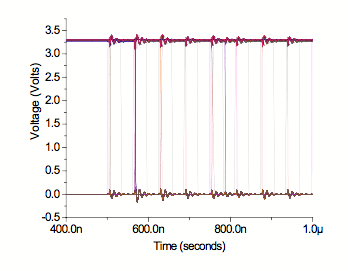
\includegraphics{preset} 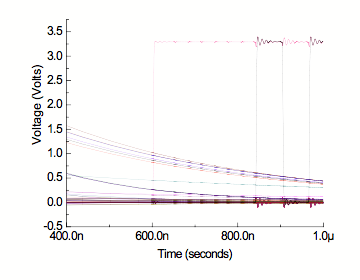
\includegraphics{nopreset} }
  \caption[Example result with and without an Initial Condition (IC).]
  {Example result with (left) and without (right) an IC on the output.  
NOTE:	The preset example, with an IC, starts in the initial state directly out of the DCOP calculation, while the non-preset example requires a long transient to equilibrate.  \label{preset_vs_nopreset}}
\end{figure}

\newpage
\section{Device Level IC= Specification}
\label{IC_equals_spec}

\index{IC=}

Many devices in \Xyce{} support setting initial junction voltage
conditions on the device instance line with the \texttt{IC=} keyword.
This is frequently used to set the state of digital circuits.
Figure~\ref{IC_Netlist_1} presents a simple inverter example
demonstrating the use of \texttt{IC=} on a BSIMSOI device.  In this
example, the two initial conditions are specified as a vector, which is the
preferred syntax.  The initial conditions can also be specified separately
(e.g., \texttt{IC1=}2  \texttt{IC2=}0).

While many circuit simulators have a similar \texttt{IC=} capability,
\Xyce{} implementation differs in some important respects.  For any
device with an \texttt{IC=} statement, \Xyce{} enforces the junction
drop during the operating point computation by inserting a voltage
source in parallel with the device junction.  \Xyce{} then applies the
parallel voltage source through the DCOP calculation, and then removes
it prior to the beginning of the transient.  This strongly enforces
the requested junction drop, meaning that if the DCOP converges, the
requested voltage drop will be in the solution and the entire circuit
solution will be consistent with that voltage drop.  Many other
circuit codes apply \texttt{IC=} as a weaker constraint, with the
intent of improving DCOP calculation robustness.

\texttt{IC=} can be applied to the following devices:  BSIM3, BSIM4, BSIMSOI,
Capacitor, Inductor and Digital Behavioral Devices (U and Y).

In the case of the capacitor, initial conditions specified via an
\texttt{IC=} parameter are also applied as an initial condition for
transients in the case that the user has used a \texttt{NOOP} or
\texttt{UIC} option on a transient line, bypassing the operating point
calculation.  In this case only, the initial condition is not enforced by
the addition of a voltage source, but rather by a weaker constraint
similar to the method used by other SPICE-type simulators.

\begin{figure}[htbp]
\begin{centering}
\shadowbox{
\begin{minipage}{0.8\textwidth}
\begin{vquote}
MOS LEVEL=10 INVERTER WITH IC=

.subckt INV IN OUT VDD GND
MN1 OUT IN GND GND GND NMOS w=4u  l=0.15u \color{XyceRed}IC=2,0 \color{black}
MP1 OUT IN VDD GND VDD PMOS w=10u l=0.15u 
.ends

.tran 20ns 30us
.print tran v(vout) {v(in)+1.0} v(1)

VDDdev  VDD 0 2V
RIN IN  1 1K
VIN1  1 0  2V PULSE (2V 0V 1.5us 5ns 5ns 1.5us 3.01us)
R1    VOUT  0  10K
C2    VOUT  0  0.1p
XINV1 IN VOUT VDD 0 INV
.MODEL NMOS NMOS ( LEVEL = 10 )
.MODEL PMOS PMOS ( LEVEL = 10 )

.END
\end{vquote}
\end{minipage}
}
\caption[Example netlist with device-level IC=.]{Example netlist with device-level IC=.\label{IC_Netlist_1}}
\end{centering}
\end{figure}

\newpage
\section{.IC and .DCVOLT Initial Condition Statements}
\label{IC_statement_spec}

\index{\texttt{.IC}}
\index{\texttt{.DCVOLT}}

\texttt{.IC} and \texttt{.DCVOLT} are equivalent methods for
specifying initial conditions.  How \Xyce{} applies them, however,
depends on whether the \texttt{UIC} parameter, discussed in a following
subsection, is present on the \texttt{.TRAN} line.  
If \texttt{UIC} is not specified, then \Xyce{}
applies the conditions specified by \texttt{.IC} and
\texttt{.DCVOLT} statements throughout the DCOP phase, ensuring the
specified values will be the solved values at the end of the DCOP
calculation.  \Xyce{} allows unspecified variables to find their
computed values, consistent with the imposed voltages.

\begin{figure}[htbp]
\begin{centering}
\shadowbox{
\begin{minipage}{0.8\textwidth}
\begin{vquote}
RC circuit
\color{XyceRed}.ic v(1)=1.0\color{black}
c1 1 0 1uF 
R1 1 2 1K
v1 2 0 0V
.print tran v(1)
.tran 0 5ms
.options timeint reltol=1e-6 abstol=1e-6
.end
\end{vquote}
\end{minipage}
}
\caption[Example netlist with \texttt{.IC}.]{Example netlist with \texttt{.IC}. 
NOTE:	Without the \texttt{.IC} statement, the capacitor is not given an initial charge, and the transient signals are flat. With the \texttt{.IC} statement, it has an initial charge, which then decays in transient. Without the \texttt{.IC} statement, the capacitor is not given an initial charge, and the signals in transient are all flat.  With the \texttt{.IC} statement, it has an initial change which then decays in transient.  \label{IC_Netlist_2}}
\end{centering}
\end{figure}

If \texttt{UIC} is specified on the \texttt{.TRAN} line, then \Xyce{}
skips the DCOP calculation altogether, and uses the values specified
on \texttt{.IC} and \texttt{.DCVOLT} lines as the initial values for
the transient calculation.  Unspecified values are set to zero.

For the \texttt{UIC} and non-\texttt{UIC} cases, \Xyce{} ignores
specified values that do not correspond to existing circuit variables.

Finally, the \texttt{.IC} capability can only set voltage values, not current values.

\subsection{Syntax}

\begin{vquote}
.IC V(node1) = val1 <V(node2) = val2> ...
.DCVOLT V(node1) = val1 <V(node2) = val2> ...
\end{vquote}

where:  \emph{val1, val2, ...} specify nodal voltages and \emph{node1, node2, ...} specify node numbers.

\subsection{Example}

\begin{vquote}
.IC V(1) = 2.0  V(A) = 4.5
.DCVOLT  1 2.0 A 4.5
\end{vquote}

Fig.~\ref{IC_Netlist_2} provides a more complete example (showing a full netlist).

\newpage
\section{.NODESET Initial Condition Statements}
\label{NODESET_statement_spec}

\index{\texttt{.NODESET}}

\texttt{.NODESET} is similar to \texttt{.IC}, except that \Xyce{}
enforces the specified conditions less strongly.  For
\texttt{.NODESET} simulations, \Xyce{} performs {\em two} nonlinear
solves for the DCOP condition.  For the first solve, \Xyce{} enforces
the \texttt{.NODESET} values throughout the solve, similar to
\texttt{.IC}.  For the second solve, \Xyce{} uses the result of the
first solve as an initial guess, and allows all the values to float
and eventually obtain their unconstrained, self-consistent values.  As
such, the computed values will not necessarily match the specified
values.  

If used with \texttt{UIC} or \texttt{NOOP}~\ref{UIC_NOOP_spec}, \texttt{.NODESET} 
behaves the same as \texttt{.IC} and \texttt{.DCVOLT}. 

\subsection{Syntax}

\begin{vquote}
.NODESET V(node1) = val1 <V(node2) = val2> ...
.NODESET node1 val1 <node2 val2>
\end{vquote}

where:  \emph{val1, val2, ...} specify nodal voltages and \emph{node1, node2, ...} specify node numbers.

\subsection{Example}

\begin{vquote}
.NODESET V(1) = 2.0  V(A) = 4.5
.NODESET  1 2.0 A 4.5
\end{vquote}

\newpage
\section{.SAVE Statements}
\label{SAVE_statement_spec}

\index{\texttt{.SAVE}}
\index{\texttt{.INCLUDE}}

\Xyce{} stores operating point information using  \texttt{.SAVE} statements, and can then 
reuse that information to start subsequent transient simulations.  Using \texttt{.SAVE} results in
solution data being stored in a text file, comprised of \texttt{.NODESET} or \texttt{.IC}
statements.  This file can be applied to other simulations using \texttt{.INCLUDE}.

The \texttt{.SAVE} syntax is as follows:

\begin{vquote}
.SAVE [TYPE=<IC|NODESET>] [FILE=<filename>] [LEVEL=<all|none>]
+ [TIME=<save_time>]
\end{vquote}

where:

The \textrmb{TYPE} can be set to \texttt{NODESET} or \texttt{IC}.  By
default, it will be \texttt{NODESET}.  

The \textrmb{FILE} is the user-specified output file name for the output file.
If this is not specified, \Xyce{} uses \texttt{\emph{netlist.cir}.ic}.

The \textrmb{LEVEL} is an HSPICE compatibility parameter.  \Xyce{} supports
\texttt{ALL} and \texttt{NONE}. If \texttt{NONE} is specified, then no save
file is created. The default \textrmb{LEVEL} is \texttt{ALL}.

\textrmb{TIME} is an HSPICE compatibility parameter. This is unsupported
in \Xyce{}. \Xyce{} outputs the save file only at time=0.0.

\newpage
\section{UIC and NOOP}
\label{UIC_NOOP_spec}
\index{\texttt{.TRAN}!\texttt{UIC}} \index{\texttt{.TRAN}!\texttt{NOOP}}
As noted earlier, the \texttt{UIC} key word on the \texttt{TRAN} line
will disable the DCOP calculation, and result in \Xyce{} immediately
going to transient.  If the user specifies \texttt{.IC} or
\texttt{.NODESET}, then the transient
calculation will use the specified initial values as the initial
starting point.  The \texttt{NOOP} keyword works exactly the same way
as \texttt{UIC}.

\begin{figure}[htbp]
\begin{centering}
\shadowbox{
\begin{minipage}{0.8\textwidth}
\begin{vquote}
pierce oscillator
c1 1 0 100e-12
c2 3 0 100e-12
c3 2 3 99.5e-15
c4 1 3 25e-12
l1 2 4 2.55e-3  
r1 1 3 1e5
r2 3 5 2.2e3
r3 1 4 6.4
v1 5 0 12
Q1 3 1 0 NBJT
.MODEL NBJT NPN (BF=100)
.print tran  v(2) v(3)

.tran 1ns 1us  \color{XyceRed}UIC\color{black}
.ic v(2)=-10000.0 v(5)=12.0
\end{vquote}
\end{minipage}
}
\caption[Example netlist with UIC.] {Example netlist with UIC. 
NOTE: This circuit is a pierce oscillator, which only oscillates if
the operating point calculation is skipped.  If the \texttt{.IC} statement is
not included, the oscillator will take a long time to achieve its
steady-state amplitude.  By including the \texttt{.IC} statement, the
amplitude of node 2 is preset to a value close to its final
steady-state amplitude.  The transient in this example only runs for
10 cycles as a demonstration.  In general, the time scales for this
oscillator are much longer and require millions of
cycles.  \label{UIC_Netlist}}
\end{centering}
\end{figure}

\subsection{Example}
\begin{vquote}
.tran 1ns 1us  UIC
.tran 1ns 1us  NOOP
\end{vquote}

Some circuits, particularly oscillator circuits, will only function properly if the operating point calculation
is skipped, as they need an inconsistent initial state to oscillate.  Figure~\ref{UIC_Netlist} presents a Pierce oscillator example.

%%% Local Variables:
%%% mode: latex
%%% End:

% END of Xyce_UG_InitialConditions.tex ************

\cleardoublepage
% Sandia National Laboratories is a multimission laboratory managed and
% operated by National Technology & Engineering Solutions of Sandia, LLC, a
% wholly owned subsidiary of Honeywell International Inc., for the U.S.
% Department of Energy’s National Nuclear Security Administration under
% contract DE-NA0003525.

% Copyright 2002-2021 National Technology & Engineering Solutions of Sandia,
% LLC (NTESS).

%%-------------------------------------------------------------------------
%% Purpose        : Main LaTeX Xyce Users' Guide
%% Special Notes  : Graphic files (pdf format) work with pdflatex.  To use
%%                  LaTeX, we need to use postcript versions.  Not sure why.
%% Creator        : Keith Santarelli
%% Creation Date  : 12/17/2007
%%
%%-------------------------------------------------------------------------

% -------------------------------------------------------------------------
% .PREPROCESS statements Chapter --------------------------------
% -------------------------------------------------------------------------

\chapter{Working with .PREPROCESS Commands}
\label{Preprocess_Chap}
\index{\texttt{.PREPROCESS}}
%%%%%%%%%%%%%%HAVE TO ADD LABEL TO TABLE OF CONTENTS, OR INDEX, OR SOMETHING??

%\index{}
%%%%%%%%%%%%%%HAVE TO ADD IN INDEXING STUFF AT SOME POINT, TOO!!!!!

\chapteroverview{Chapter Overview}
{
This chapter includes the following sections:
\begin{XyceItemize}
\item Section~\ref{PP_Intro}, {\em Introduction}
\item Section~\ref{PP_gndsyn}, {\em Ground Synonym Replacement}
\item Section~\ref{PP_removeunused}, {\em Removal of Unused Components}
\item Section~\ref{PP_dangling}, {\em Adding Resistors to Dangling Nodes}

\end{XyceItemize}
}

\section{Introduction}
\label{PP_Intro}

In an effort to make \Xyce{} more compatible with other commercial circuit 
simulators (e.g., HSPICE), some optional tools have been added to increase the netlist processing capabilities of \Xyce{}.  These options, which occur toward
the beginning of a simulation, have been incorporated not only to make 
\Xyce{} more compatible with different (i.e. non-\Xyce{}) netlist syntaxes, but also 
to help detect and remove certain singular netlist configurations that can often 
cause a \Xyce{} simulation to fail.  Because all of the commands described 
in this section occur as a precursory step to setting up a \Xyce{} simulation, they are 
all invoked in a netlist file via the keyword \texttt{.PREPROCESS}.  This 
chapter describes each of the different functionalities that can be invoked 
via a \texttt{.PREPROCESS} statement in detail and provides examples to illustrate 
their use.



%%%%%%%%%%%%%%%%%%%%%%%%%%%%%%%%%%%
%%GROUND SYNONYM CHECKING
%%%%%%%%%%%%%%%%%%%%%%%%%%%%%%%%%%%

\section{Ground Synonym Replacement}
\label{PP_gndsyn}
\index{\texttt{.PREPROCESS}!\texttt{REPLACEGROUND}}
In certain versions of SPICE, keywords such as \texttt{GROUND}, \texttt{GND}, and 
\texttt{GND!} can be used as node names in a netlist file to represent the ground 
node of a circuit.  \Xyce{}, however, only recognizes node \texttt{0} as an official
name for ground.  Hence, if any of the prior node names is encountered in a 
netlist file, \Xyce{} will treat these as different nodes from ground.  To 
illustrate this point, consider the netlist of figure\ \ref{fig:nlgndrepl2}.  
When the node \texttt{Gnd} is encountered in the definition of resistor \texttt{R3}, 
\Xyce{} instantiates this as a new node.  The schematic diagram corresponding to
this netlist (figure\ \ref{fig:gndreplace2}) shows that the resistor 
\texttt{R3} is ``floating'' between node \texttt{2} and a node with only a 
single device connection, node \texttt{Gnd}.  When \Xyce{} executes the netlist of figure\ 
\ref{fig:nlgndrepl2}, the voltage \texttt{V(2)} will evaluate to 0.5V.  

\begin{figure}[htbp]
\begin{centering}
\shadowbox{
\begin{minipage}{0.8\textwidth}
\begin{vquote}
Circuit with "floating" resistor R3

V1 1 0 1
R1 1 2 1
R2 2 0 1
R3 2 Gnd 1

.DC V1 1 1 0.1
.PRINT DC V(2)
.END
\end{vquote}
\end{minipage}
}
\caption[Example netlist -- \texttt{Gnd} treated {\em different}
from node \texttt{0}.] {Example netlist where \texttt{Gnd} is treated as being {\em different}
from node \texttt{0}.}
\label{fig:nlgndrepl2}
\end{centering}
\end{figure}

\begin{figure}
\centering{\input{gndreplace2.latex}}
\caption[Circuit diagram corresponding to figure\ 
\ref{fig:nlgndrepl2}.] {Circuit diagram corresponding to the netlist of figure\ 
\ref{fig:nlgndrepl2} where node \texttt{Gnd} is treated as being {\em different} 
from node \texttt{0}.} 
\label{fig:gndreplace2}
\end{figure}

If one would rather treat \texttt{Gnd} the same as node \texttt{0} in the above example, use the  figure\ 
\ref{fig:nlgndrepl1} netlist instead.  When the statement \texttt{.PREPROCESS REPLACEGROUND
TRUE} is present in a netlist, \Xyce{} will treat any nodes named \texttt{GND}, \texttt{GND!}, \texttt{GROUND}, or any capital/lowercase variant of these keywords (e.g., \texttt{gROunD}) as synonyms
for node \texttt{0}.  Hence, according to \Xyce{}, the figure\ \ref{fig:nlgndrepl1} netlist corresponds to figure\ 
\ref{fig:gndreplace1} schematic diagram, and the voltage \texttt{V(2)} will evaluate to 0.33V.

\begin{figure}[htbp]
\begin{centering}
\shadowbox{
\begin{minipage}{0.8\textwidth}
\begin{vquote}

Circuit where resistor R3 does *not* float

V1 1 0 1
R1 1 2 1
R2 2 0 1
R3 2 Gnd 1

.PREPROCESS REPLACEGROUND TRUE

.DC V1 1 1 0.1
.PRINT DC V(2)
.END
\end{vquote}
\end{minipage}
}
\caption[Example netlist --- \texttt{Gnd} as a synonym for node 
\texttt{0}.] {Example netlist where \texttt{Gnd} is treated as a synonym for node 
\texttt{0}.}
\label{fig:nlgndrepl1}
\end{centering}
\end{figure}

\begin{figure}
\centering{\input{gndreplace1.latex}}
\caption [Circuit diagram corresponding to figure\ \ref{fig:nlgndrepl1}.]{Circuit diagram corresponding to figure\ \ref{fig:nlgndrepl1} where 
node \texttt{Gnd} is treated as a synonym for node \texttt{0}.} 
\label{fig:gndreplace1}
\end{figure}

NOTE:	Only one \texttt{.PREPROCESS REPLACEGROUND} statement is allowed per netlist file. This constraint prevents the user from setting \texttt{REPLACEGROUND} to \texttt{TRUE} on one line and then to \texttt{FALSE} on 
another line.  Also, there is no way to differentiate between different keywords. So, for example, it is not possible to treat \texttt{GROUND} as a synonym for node \texttt{0} while allowing \texttt{GND} to represent an independent
node).  If \texttt{REPLACEGROUND} is set to \texttt{TRUE}, \Xyce{} will treat {\em both} of these keywords as node \texttt{0}.



%%%%%%%%%%%%%%%%%%%%%%%%%%%%%%%%%%%
%%REMOVING UNUSED COMPONENTS
%%%%%%%%%%%%%%%%%%%%%%%%%%%%%%%%%%%

\section{Removal of Unused Components}
\label{PP_removeunused}
\index{\texttt{.PREPROCESS}!\texttt{REMOVEUNUSED}}

Consider a slight variant of the circuit in figure\ \ref{fig:nlgndrepl1} with
the netlist given in figure\ \ref{fig:nlunused1}.  Here, the resistor \texttt{R3}
is connected in a peculiar configuration:  both terminals of the resistor are 
tied to the same circuit node, as is illustrated in figure\ \ref{fig:unused1}.
Clearly, the presence of this resistor has no effect on the other voltages and
currents in the circuit since, by the very nature of its configuration, it has
no voltage across it and, hence, does not draw any current.  Therefore, in 
some sense, the component can be considered as ``unused.''  The presence of a resistor such as \texttt{R3} is rarely or never introduced by design, rather the presence of such components is the 
result of either human or automated error during netlist creation.

\begin{figure}[htbp]
\begin{centering}
\shadowbox{
\begin{minipage}{0.8\textwidth}
\begin{vquote}
Circuit with an unused resistor R3

V1 1 0 1
R1 1 2 1
R2 2 0 1
R3 2 2 1

.DC V1 1 1 0.1
.PRINT DC V(2)
.END
\end{vquote}
\end{minipage}
}
\caption[Netlist with a resistor with terminals both the
same node.] {Netlist with a resistor \texttt{R3} whose device terminals are both the
same node (node \texttt{2}).}
\label{fig:nlunused1}
\end{centering}
\end{figure}

\begin{figure}
\centering{\input{unused1.latex}}
\caption[Circuit of figure\ \ref{fig:nlunused1}.] {Circuit of figure\ \ref{fig:nlunused1} containing a resistor \texttt{R3} whose terminals are tied to the same node (node \texttt{2}).} 
\label{fig:unused1}
\end{figure}

While the presence of the resistor \texttt{R3} in figure\ \ref{fig:nlgndrepl1} does not 
change the behavior of the circuit, it adds an additional component to 
the netlist  \Xyce{} must include when solving for the voltages and 
currents in the circuit.  If the number of such components in a given netlist
is large, it is potentially desirable to remove them from the
netlist to ease the burden on \Xyce's solver engines.  This, in turn, can help
to avoid possible convergence issues.  For example, even though the netlist in
figure\ \ref{fig:nlunused1} will run properly in \Xyce{}, the netlist of figure\ 
\ref{fig:nlunused3} will abort.  The voltage source \texttt{V2} attempts to place
a 1V difference between its two device terminals; however, as both nodes of
the voltage source are the same, the voltage source is effectively shorted.

\begin{figure}[htbp]
\begin{centering}
\shadowbox{
\begin{minipage}{0.8\textwidth}
\begin{vquote}
Circuit with improperly connected voltage source V2

V1 1 0 1
R1 1 2 1
R2 2 0 1
V2 2 2 1

.DC V1 1 1 0.1
.PRINT DC V(2)
.END
\end{vquote}
\end{minipage}
}
\caption[Circuit with an improperly connected voltage source.] {Circuit with an improperly connected voltage source \texttt{V2}.}
\label{fig:nlunused3}
\end{centering}
\end{figure}

\Xyce{} includes the following command to prevent similar situations:

\texttt{.PREPROCESS REMOVEUNUSED <component list>}

where \texttt{<component list>} is a list of device types separated by commas.
For each device type specified in the list, \Xyce{} checks for instances of
that device type for which all of the device's terminals are connected to the
same node.  If such a device is found, \Xyce{} removes that device from the
netlist.  For instance, when executing the netlist of figure\ \ref{fig:nlunused2},
\Xyce{} will seek out such devices and remove them from the netlist.  This causes the
resistor \texttt{R3} to be removed from the netlist. Figure\ \ref{fig:unused2} presents the schematic of the 
resulting \Xyce{}-simulated circuit.  
NOTE:	The presence of  ``\texttt{C}'' in the \texttt{REMOVEUNUSED} statement does
not cause \Xyce{} to abort even though there are no capacitors in the netlist.
Also, as in the case of a \texttt{REPLACEGROUND} statement, only one 
\texttt{.PREPROCESS REMOVEUNUSED} line may be present in a netlist, or \Xyce{} will abort.

Table \ref{tbl:removeunusedtbl} lists devices that can be removed via a \texttt{REMOVEUNUSED} 
statement.  In the case of MOSFETs and BJTs, three device terminals must be the same (the gate, source,
and drain in the case of a MOSFET; the base, collector, and emitter in the
case of a BJT) to remove either device from the netlist.

\begin{figure}[htbp]
\begin{centering}
\shadowbox{
\begin{minipage}{0.8\textwidth}
\begin{vquote}
Circuit with improperly connected voltage source V2

V1 1 0 1
R1 1 2 1
R2 2 0 1
R3 2 2 1

.PREPROCESS REMOVEUNUSED R,C

.DC V1 1 1 0.1
.PRINT DC V(2)
.END
\end{vquote}
\end{minipage}
}
\caption{Circuit with an ``unused'' resistor R3 removed from the 
netlist.}
\label{fig:nlunused2}
\end{centering}
\end{figure}

\begin{figure}[h]
\centering{\input{unused2.latex}}
\caption[Circuit of figure\ \ref{fig:nlunused2}.] {Circuit of figure\ \ref{fig:nlunused2} where resistor R3 has been removed via the \texttt{.PREPROCESS REMOVEUNUSED} statement.} 
\label{fig:unused2}
\end{figure}

\LTXtable{0.5\textwidth}{removeunusedtbl}



%%%%%%%%%%%%%%%%%%%%%%%%%%%%%%%%%%%%%%%%%%%%%%
%%ADDING RESISTORS TO NO-DC-PATH AND 
%%CONN-TO-ONE-TERMINAL NODES
%%%%%%%%%%%%%%%%%%%%%%%%%%%%%%%%%%%%%%%%%%%%%%

\section{Adding Resistors to Dangling Nodes}
\label{PP_dangling}
\index{\texttt{.PREPROCESS}!\texttt{ADDRESISTORS}}
Consider the netlist of figure\ \ref{fig:nldangling1} and the corresponding
schematic of figure\ \ref{fig:dangle1}.  Nodes \texttt{3} and \texttt{4} of the 
netlist are what we will henceforth refer to as {\em dangling nodes}.  We say
that node \texttt{4} dangles because it is only connected to the terminal of a
single device, while we say that node \texttt{3} dangles because it has no DC
path to ground.  The first of these situations---connection to a single 
device terminal only---can arise, for example, in a netlist which contains 
nodes representing output pins that are not connected to a load device.  For 
instance, the resistance \texttt{R2} in figure\ \ref{fig:nldangling1} could 
represent the resistance of an output pin of a package that is meant to drive 
resistive loads.  Hence, an actual physical implementation of the circuit of 
figure\ \ref{fig:dangle1} would normally include a resistor between node \texttt{4} 
and ground, but, in creating the netlist, the presence of such an output load 
has been (either intentionally or unintentionally) left out.

\begin{figure}[htbp]
\begin{centering}
\shadowbox{
\begin{minipage}{0.8\textwidth}
\begin{vquote}
Circuit with two dangling nodes, nodes 3 and 4

V1 1 0 1
R1 1 2 1
C1 2 3 1 
C2 3 0 1
R2 2 4 1

.DC V1 0 1 0.1
.PRINT DC V(2)
.END
\end{vquote}
\end{minipage}
}
\caption[Netlist of circuit with two dangling nodes.] {Netlist of circuit with two dangling nodes, nodes \texttt{3} and 
\texttt{4}.}
\label{fig:nldangling1}
\end{centering}
\end{figure}

\begin{figure}[h]
\centering{\input{dangle1.latex}}
\caption{Schematic of netlist in figure\ \ref{fig:nldangling1}.} 
\label{fig:dangle1}
\end{figure}

The second situation---where a node has no DC path to ground---is sometimes an
effect that is purposely incorporated into a design (e.g., the design of
switched capacitor integrators (e.g., see \cite{JohnsMartin}, chapter 10), but
oftentimes it is also the result of some form of error in the process of
creating the netlist.  For instance, when graphical user interfaces (GUIs) are
used to create circuit schematics that are then translated into netlists via
software, one very common unintentional error is to fail to connect two nodes
that are intended to be connected.  To illustrate this point, consider the
schematic of figure\ \ref{fig:dangle3}.  The schematic seems to indicate that
the lower terminal of resistor \texttt{R2} should be connected to node
\texttt{3}. This is not the case as there is a small gap between node
\texttt{3} and the line intended to connect node \texttt{3} to the resistor.
Such an error can often go unnoticed when creating a schematic of the netlist
in a GUI.  Thus, when the schematic is translated into a netlist file, the
resulting netlist would {\em not} connect the resistor to node \texttt{3} and
would instead create a new node at the bottom of the resistor, resulting in the
circuit depicted in figure\ \ref{fig:dangle1}.  

While neither of the previous situations is necessarily threatening (\Xyce{}
will run the figure\ \ref{fig:nldangling1} netlist successfully to completion),
there are times when it is desirable to somehow make a dangling node {\em not}
dangle.  For instance, returning to the example in which the resistor
\texttt{R2} represents the resistance of an output pin, one may want to
simulate the circuit when a 1K load is attached between node \texttt{4} and
ground in figure\ \ref{fig:dangle1}.  In the case where a node has no DC path
to ground, the situation is slightly more dangerous if, for instance, the node
in question is also connected to a high-gain device such as the gate of a
MOSFET.  As the DC gate bias has a great impact on the DC current traveling
through the drain and source of the transistor, not having a well-defined DC
gate voltage can greatly degrade the simulated performance of the circuit.

In both prior examples, the only true way to ``fix'' each of these issues is to
find all dangling nodes in a particular netlist file and augment the netlist
at/near these nodes to obtain the desired behavior.  If, however, the number of
components in a circuit is very large (say on the order of hundreds of
thousands of components), manually augmenting the netlist file for each
dangling node becomes a practical impossibility if the number of such nodes is
large.  

Hence, it is desirable for \Xyce{} to be capabable of automatically augmenting
netlist files so as to help remove dangling nodes from a given netlist.  The
command \texttt{.PREPROCESS ADDRESISTORS} is designed to do just this. Assuming
the netlist of figure\ \ref{fig:nldangling2} is stored in the file
\texttt{filename}, the \texttt{.PREPROCESS ADDRESISTORS} statements will cause
\Xyce{} to create a new netlist file called \texttt{filename\_xyce.cir}
(depicted in figure\ \ref{fig:nlnotdangling}).  The line \texttt{.PREPROCESS
ADDRESISTORS NODCPATH 1G} instructs \Xyce{} to create a copy of the netlist
file containing a set of resistors of value 1~G$\mathsf{\Omega}$ that are
connected between ground and the nodes that did not have a DC path to ground.
Similarly, the line \texttt{.PREPROCESS ADDRESISTORS ONETERMINAL 1M} instructs
\Xyce{} to add to the same netlist file a set of resistors of value
1~M$\mathsf{\Omega}$ that are connected between ground and devices that are
connected to only one terminal.  The resistor \texttt{RNODCPATH1} in figure\
\ref{fig:nlnotdangling} achieves the first of these goals while
\texttt{RONETERM1} achieves the second.  Figure\ \ref{fig:dangle2} shows a
schematic of the resulting circuit represented by the netlist in figure\
\ref{fig:nlnotdangling}.

\begin{figure}[h]
\centering{\input{dangle3.latex}}
\caption[Schematic  with an incomplete connection.] {Schematic of a circuit with an incomplete connection between the 
resistor \texttt{R2} and node \texttt{3}.} 
\label{fig:dangle3}
\end{figure}

\begin{figure}[htbp]
\begin{centering}
\shadowbox{
\begin{minipage}{0.8\textwidth}
\begin{vquote}
Circuit with two dangling nodes, nodes 3 and 4

V1 1 0 1
R1 1 2 1
C1 2 3 1 
C2 3 0 1
R2 2 4 1

.PREPROCESS ADDRESISTORS NODCPATH 1G
.PREPROCESS ADDRESISTORS ONETERMINAL 1M

.DC V1 0 1 0.1
.PRINT DC V(2)
.END
\end{vquote}
\end{minipage}
}
\caption[Netlist of circuit with two dangling nodes with \texttt{.PREPROCESS ADDRESISTORS} statements.] {Netlist of circuit with two dangling nodes, nodes \texttt{3} and \texttt{4}, with \texttt{.PREPROCESS ADDRESISTORS} statements.}
\label{fig:nldangling2}
\end{centering}
\end{figure}



\begin{figure}[htbp]
\begin{centering}
\shadowbox{
\begin{minipage}{0.8\textwidth}
\begin{vquote}
XYCE-generated Netlist file copy:  TIME='07:32:31 AM' 
* DATE='Dec 19, 2007' 
*Original Netlist Title:  

*Circuit with two dangling nodes, nodes 3 and 4.


V1 1 0 1
R1 1 2 1
C1 2 3 1 
C2 3 0 1
R2 2 4 1

*.PREPROCESS ADDRESISTORS NODCPATH 1G
*Xyce:  ".PREPROCESS ADDRESISTORS" statement 
* automatically commented out in netlist copy.
*.PREPROCESS ADDRESISTORS ONETERMINAL 1M
*Xyce:  ".PREPROCESS ADDRESISTORS" statement 
* automatically commented out in netlist copy.

.DC V1 0 1 0.1
.PRINT DC V(2)


*XYCE-GENERATED OUTPUT:  Adding resistors between ground 
* and nodes connected to only 1 device terminal:

RONETERM1 4 0 1M


*XYCE-GENERATED OUTPUT:  Adding resistors between ground 
* and nodes with no DC path to ground:

RNODCPATH1 3 0 1G

.END
\end{vquote}
\end{minipage}
}
\caption[Output file resulting from  
\texttt{.PREPROCESS ADDRESISTOR} statements for figure~\ref{fig:dangle3}.] {Output file \texttt{filename\_xyce.cir} which results from the 
\texttt{.PREPROCESS ADDRESISTOR} statements for the netlist of figure\ 
\ref{fig:dangle3} (with assumed file name \texttt{filename}).}
\label{fig:nlnotdangling}
\end{centering}
\end{figure}



\begin{figure}[h]
\centering{\input{dangle2.latex}}
\caption[Schematic corresponding to figure\ 
\ref{fig:nlnotdangling}.] {Schematic corresponding to the \Xyce{}-generated netlist of figure\ 
\ref{fig:nlnotdangling}.} 
\label{fig:dangle2}
\end{figure}

Some general comments regarding the use of \texttt{.PREPROCESS ADDRESISTOR} 
statements include:

\begin{itemize}
\item \Xyce{} does not terminate immediately after the netlist file is created.
In other words, if \Xyce{} is run on the \texttt{filename} of figure\ 
\ref{fig:nldangling2} netlist, it will attempt to execute this netlist as given 
(i.e., it tries to simulate the circuit of figure\ \ref{fig:dangle1}) and 
generates the file \texttt{filename\_xyce.cir} as a byproduct.  It is important to
point out that the resistors that are added at the bottom of the netlist 
file \texttt{filename\_xyce.cir} do {\bf not} get added to the original netlist
when \Xyce{} is running on the file \texttt{filename}.  If one wishes to simulate
\Xyce{} with these resistors in place, one must run \Xyce{} on 
\texttt{filename\_xyce.cir} explicitly.

\item The naming convention for resistors which connect to ground nodes which 
do not have a DC path to ground is \texttt{RNODCPATH<i>}, where \texttt{i} is an 
integer greater than 0; the naming convention is similar for nodes which are 
connected to only one device terminal (i.e., of the form \texttt{RONETERM<i>}).   
\Xyce{} will not change this naming convention if a 
resistor with one of the above names already exists in the netlist.  

Hence, if a resistor named \texttt{RNODCPATH1} exists in netlist file 
\texttt{filename}, and \Xyce{} detects there is a node in this netlist file 
that has no DC path to ground, \Xyce{} will add {\em another} resistor with name 
\texttt{RNODCPATH1} to the netlist file \texttt{filename\_xyce.cir} (assuming that 
either \texttt{.PREPROCESS ADDRESISTORS NODCPATH} or \texttt{.PREPROCESS ADDRESISTORS
ONETERMINAL} are present in \texttt{filename}).  If \Xyce{} is subsequently run on 
\texttt{filename\_xyce.cir}, it will exit in error due to the presence of two 
resistors with the same name.

\item Commands \texttt{.PREPROCESS ADDRESISTORS NODCPATH}  and 
\texttt{.PREPROCESS} \newline \texttt{ADDRESISTORS ONETERMINAL} do {\bf not} have to be 
simultaneously present in a netlist file.  The presence of either command will
generate a file \texttt{filename\_xyce.cir}, and the presence of both will not
generate two separate files.  As with other \texttt{.PREPROCESS} commands, 
however, a netlist file is allowed to contain only one \texttt{NODCPATH} and
one \texttt{ONETERMINAL} command each.  If multiple \texttt{NODCPATH} and/or 
\texttt{ONETERMINAL} lines are found in a single netlist file, \Xyce{} will exit in
error.

\item It is possible that a single node can have no DC path to ground 
{\em and} be connected to only one device terminal.  If a \texttt{NODCPATH}
and \texttt{ONETERMINAL} command are present in a given netlist file, {\bf only}
the resistor corresponding to the \texttt{ONETERMINAL} command is added to 
the netlist file \texttt{filename\_xyce.cir} and the resistor corresponding to 
the \texttt{NODCPATH} command is omitted.  If a \texttt{NODCPATH} command is 
present but a \texttt{ONETERMINAL} command is not, then \Xyce{} will add a resistor corresponding
to the \texttt{NODCPATH} command to the netlist, as usual.
\item In generating the file \texttt{filename\_xyce.cir}, the original 
\texttt{.PREPROCESS ADDRESISTOR} statements are commented out with a warning 
message.  This is to prevent \Xyce{} from creating the file 
\texttt{filename\_xyce.cir\_xyce.cir} when the file \texttt{filename\_xyce.cir} is
run.  

NOTE:	 This feature avoids generating redundant
files.  While \texttt{filename\_xyce.cir\_xyce.cir} would be slightly different 
from \texttt{filename\_xyce.cir} (e.g., a different date and time stamp), both 
files would functionally implement the same netlist.

\end{itemize}



%%% Local Variables:
%%% mode: latex
%%% End:

% END of Xyce_UG_Preprocess.tex ************

\cleardoublepage
% Sandia National Laboratories is a multimission laboratory managed and
% operated by National Technology & Engineering Solutions of Sandia, LLC, a
% wholly owned subsidiary of Honeywell International Inc., for the U.S.
% Department of Energy’s National Nuclear Security Administration under
% contract DE-NA0003525.

% Copyright 2002-2020 National Technology & Engineering Solutions of Sandia,
% LLC (NTESS).

%%-------------------------------------------------------------------------
%% Purpose        : Main LaTeX Xyce Users' Guide
%% Special Notes  : Graphic files (pdf format) work with pdflatex.  To use
%%                  LaTeX, we need to use postcript versions.  Not sure why.
%% Creator        : Robert Hoektra, Computational Sciences, SNL
%% Creation Date  : {12/22/2003}
%%
%%-------------------------------------------------------------------------

\chapter{TCAD (PDE Device) Simulation with Xyce}
\label{PDE_Devices}
\index{PDE Device Modeling}
\index{device!PDE devices}
\index{device!TCAD devices}

\chapteroverview{Chapter Overview}
{
This chapter provides guidance for using the mesh-based device simulation
capability of \Xyce{}.  It includes the following sections:
\begin{XyceItemize}
\item Section~\ref{PDE_Introduction}, {\em Introduction}
\item Section~\ref{PDE_One_D_Example}, {\em One-Dimensional Example}
\item Section~\ref{PDE_Two_D_Example}, {\em Two-Dimensional Example}
\item Section~\ref{PDE_Doping}, {\em Doping Profile}
\item Section~\ref{PDE_Electrode}, {\em Electrodes}
\item Section~\ref{PDE_Mesh}, {\em Meshing}
\item Section~\ref{PDE_Mobility}, {\em Mobility Models}
\item Section~\ref{PDE_Bulk_Material}, {\em Bulk Materials}
\item Section~\ref{PDE_Output_Vis}, {\em Output and Visualization}
\end{XyceItemize}
}

\section{Introduction} \label{PDE_Introduction}
This chapter describes how to use the mesh-based device simulation 
functionality of \Xyce{}, which is based on the solution a coupled set of partial 
differential equations (PDEs), discretized on a mesh.
Such devices are often referred to as Technology Computer-Aided Design (TCAD) devices.
While the rest of \Xyce{} is intended to be similar to analog circuit
simulators such as SPICE, the TCAD device capability is intended to 
be similar to commercial device simulators, such as PISCES~\cite{Yu} and
DaVinci~\cite{DaVinci}.

\Xyce{} offers two different TCAD devices---a one-dimensional 
device and a two-dimensional device---and enables both to be invoked in the 
same way as a conventional lumped parameter circuit device. Generally, this 
capability is intended for very detailed simulation of semiconductor devices, 
such as diodes, bipolar transistors, and MOSFETs. As the \Xyce{} TCAD devices can
be invoked from the netlist, they can be embedded in a circuit as part of
a mixed-mode simulation.

\subsection{Equations}
Kramer~\cite{Kramer} and Selberherr~\cite{selberherr}, among others, describe 
device simulation equations. The most common formulation and the one used in 
\Xyce{}, is the drift-diffusion (DD) formulation, which consists of three coupled
PDEs (a single Poisson equation for electrostatic potential and two continuity
equations; one each for electrons and holes).

\subsubsection{Poisson equation}
The electrostatic potential $\phi$ satisfies Poisson's equation:
\begin{equation}
  -\nabla \cdot \left(\epsilon \nabla \phi(x) \right) = \rho(x) \label{poisson1}
\end{equation}
where $\rho$ is the charge density and $\epsilon$ is the permittivity of the
material.  For semiconductor devices, local carrier densities and local doping determine charge density;
\begin{equation}
  \rho(x) = q(p(x)-n(x)+C(x)) \label{poisson2}
\end{equation} 
Here, $p(x)$ is the spatially dependent concentration of holes; $n(x)$, the
concentration of electrons; and $q$, the magnitude of the charge on an electron.
$C(x)$ is the total doping concentration, which can also be represented as
$C(x)=N^+_D(x)-N^-_A(x)$, where $N^+_D$ the concentration of positively ionized
donors, $N^-_A$ the concentration of negatively ionized acceptors.

\subsubsection{Species continuity equations}
Continuity equations relate the convective derivative of the species
concentrations to the creation and destruction of particles
(``re\-com\-bin\-ation/gen\-er\-ation'').
\begin{eqnarray}
  \label{eqn:hd-cont1}
  \frac{\partial n(x)}{\partial t} + \nabla \cdot \Gamma_n &=& - R(x)\\
  \label{eqn:hd-cont2}
  \frac{\partial p(x)}{\partial t} + \nabla \cdot \Gamma_p &=& - R(x)
\end{eqnarray}
Here $n$ is the electron concentration and $p$ is the hole concentration. $R$
is the recombination rate for both species.  $\Gamma_n$ and $\Gamma_p$ are
particle fluxes for electrons and holes, respectively.  
$R$ is the recombination rate for both species, and the right hand sides are equal since
creation and destruction of carriers occurs in pairs.
The quantities $\Gamma_n$ and $\Gamma_p$ are electron and hole fluxes, and 
are determined from the following expressions:
\begin{eqnarray}
  \Gamma_n &=& n(x)\mu_n E(x) + D_n \nabla n(x)\\
  \Gamma_p &=& p(x)\mu_p E(x) + D_p \nabla p(x)
\end{eqnarray}
$\mu_n$, $\mu_p$ are mobilities for electrons and holes, and $D_n$, $D_p$
are diffusion constants. $E(x)$ is the electric field, which is given by
the gradient of the potential, or $-\partial \phi/\partial x$.

\subsection{Discretization}
\Xyce{} uses a box-integration discretization, with the Scharfetter-Gummel
method, to model the flux of charged species.  For a more-detailed description of this method, refer to ~\cite{Kramer}~\cite{selberherr}~\cite{Xyce_PDE_LDRD}.

\section{One Dimensional Example} \label{PDE_One_D_Example}
While one-dimensional device simulation has limits on its usefulness, the
simulation much faster than 2D, and it can provide reasonable physical
predictions in many situations. Two-terminal diodes are a good candidate for
one dimensional simulation, because they allow for assumptions that simplify
the specification and shorten the parameter list of the device.

Figure~\ref{One_D_Diode_Netlist} provides an example netlist for a simulation of a one-dimensional diode, while figure~\ref{One_D_Diode_Schem} shows its corresponding schematic.  This regulator circuit is based on the principle that connecting one or more diodes
in series with a resistor and a power supply will produce a relatively constant voltage.  The input voltage (node 2) is a sine wave, with a
frequency of 50 Hz and an amplitude of 1 V.  
The expected output (node 3) signal should be (mostly) flat.  
% one dimensional example netlist.
\begin{figure}
  \begin{centering}
    \shadowbox{
      \begin{minipage}{0.8\textwidth}
        \begin{vquote}
PDE Diode Regulator Circuit
VP 1 0 PULSE(0 5 0.0 2.0e-2 0.0 1.0e+20 1.2e+20)
VF 2 1 SIN(0 1 50 2.0e-2)
VT1 4 0 0V
R1 2 3 1k

\color{XyceRed} * TCAD/PDE Device
YPDE Z1 3 4 DIODE na=1.0e17 nd=1.0e17 graded=1
+ l=5.0e-4 nx=101 \color{black}
\color{XyceDarkBlue} .MODEL DIODE  ZOD  \color{black}

.TRAN 1.0e-3 12.0e-2
.print TRAN format=tecplot 
+ v(1) v(2) v(3) v(4) I(VF) I(VT1)

.options NONLIN maxstep=100 maxsearchstep=3 
+ searchmethod=2 
.options TIMEINT reltol=1.0e-3 abstol=1.0e-6 
.END
\end{vquote}
\end{minipage}
}
\caption[One-dimensional diode netlist]
{Voltage regulator circuit, using a one-dimensional TCAD diode.
Figure~\ref{One_D_outputSignal} illustrates the result of this netlist. The PDE
device instance line is in red, and the PDE device model line is in blue.
\label{One_D_Diode_Netlist} }
\end{centering}
\end{figure}

% Schematic
\begin{figure}
  \centering
  \scalebox{1.0}
  {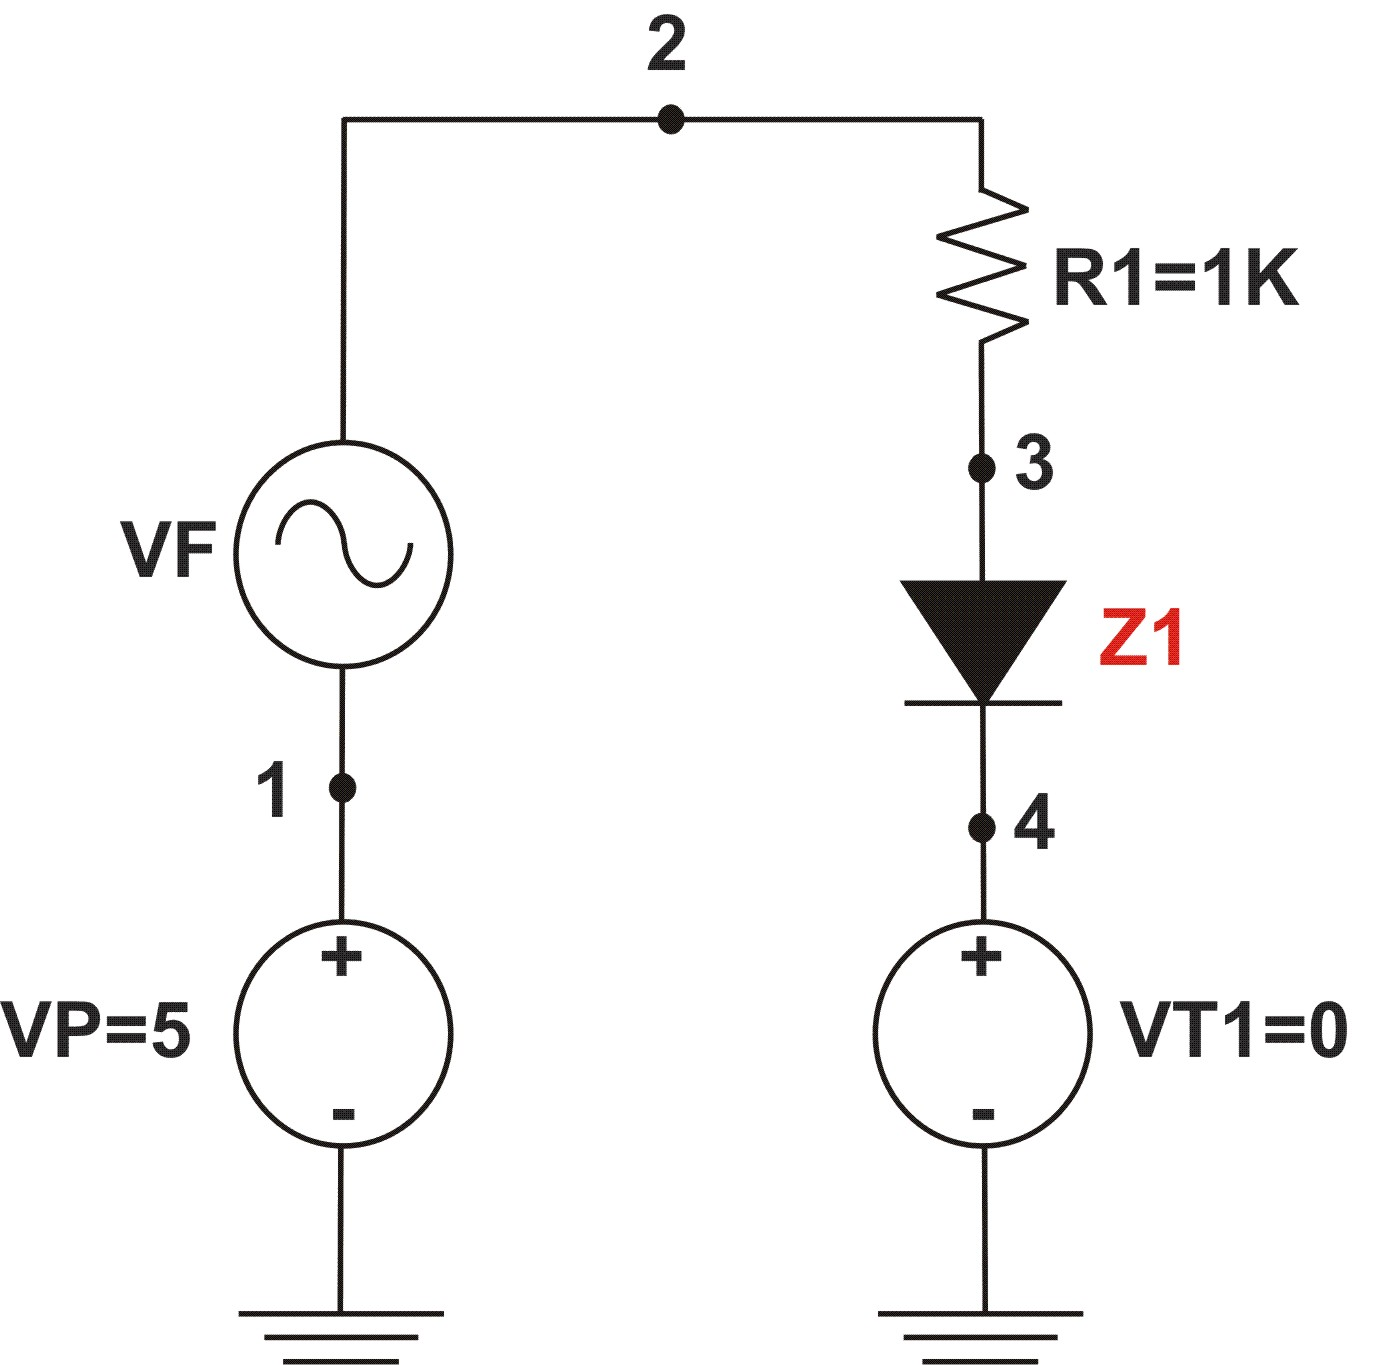
\includegraphics[width=2.300in,height= 2.270in]{diodeRegulatorSchem}}
  \caption[Voltage regulator schematic]{Voltage regulator schematic
The diode, Z1, is the PDE device in this example.\label{One_D_Diode_Schem}}
\end{figure}

\subsection{Netlist Explanation}
The model line for PDE devices serves only to set the level.  The default level
is 1, for a one-dimensional device.  Setting \texttt{level=2} will invoke
two-dimensional devices.  In this example, the level is not explicitly set, and
so \Xyce{} uses the default value which is 1.

The instance line is where most of the specific parameters are set for a
TCAD device.  In this example, the line appears as:

\texttt{YPDE Z1 3 4 DIODE na=1.0e17 nd=1.0e17 graded=1 l=5.0e-4 nx=101}

Doping parameters \texttt{na} and \texttt{nd} represent the
majority carrier doping levels on the N- and the P-sides of the
junction, respectively.  \texttt{graded=1} is also a doping parameter, and
specifies that the junction is a graded junction, rather than an abrupt
step-function junction.  \texttt{l=5.0e-4} specifies the length of
the device, in cm.  \texttt{nx=101} specifies that there are
101 mesh points, including the two endpoints.  For the one-dimensional
device, the mesh is always uniform, so the size of 
each mesh cell, $\Delta x$ will be:
\begin{equation}
  \Delta x = \frac{l}{nx-1} = \frac{\mbox{5.0e-4 cm}}{\mbox{100}} = \mbox{5.0e-6 cm}
\end{equation}
The mesh points $i=0 - 100$ will have the following locations, $x_{i}$:
\begin{eqnarray*}
  x_{i}   &=& i \Delta x\\
  x_{o}   &=& \mbox{0.0 cm} \\
  x_{1}   &=& \mbox{5.0e-6 cm} \\
  x_{2}   &=& \mbox{10.0e-6 cm} \\
          &\vdots& \\
  x_{100} &=& \mbox{5.0e-4 cm}
\end{eqnarray*}

\subsection{Boundary Conditions and Doping Profile}
The cited netlist example relies mostly on default parameters; therefore, it 
specifies nothing about electrodes, or boundary conditions, and has a minimal 
doping specification. A one-dimensional device can have only two electrodes 
connected to the circuit. The electrodes are at opposite ends of the domain, 
one at the first mesh point (\texttt{x=0.0 cm}, \texttt{i=0}) 
and the other at the opposite end of the domain, at the last mesh point 
(\texttt{x=5.0e-4 cm}, \texttt{i=101}).

The electrode associated with the first mesh point (\texttt{x=0.0 cm}) 
is connected to the \emph{second} circuit node on the instance line, 
while the electrode associated with the last mesh point (\texttt{x=l}) 
is connected to the \emph{first} circuit node on the instance line.  
For the doping used in this example, the junction is in the exact 
center of the device (\texttt{x=l/2}), and the n-side
is the region defined by \texttt{x<l/2}, and the p-side is the region defined by
\texttt{x>l/2}.  This default doping, along with the electrode-circuit connectivity,
results in a one-dimensional device that behaves like a traditional
SPICE-style diode.  For a complete discussion of how to specify
a doping profile see section~\ref{Manual_Doping}.  For a complete discussion
of how to specify electrodes (including boundary conditions), see
section~\ref{PDE_Electrode}.

\subsection{Results}
Figure~\ref{One_D_outputSignal} shows the transient behavior of this circuit.  
The voltage drop across the diode (V(3)) is nearly the same for a wide 
range of currents, and is nearly constant.  The
voltage drop (V(2)-V(3)) across the series resistor, \texttt{R1}, is much more
sensitive, and so most of the voltage 
variation of the input sine wave is accounted for by \texttt{R1}.
% Output Signal.
\begin{figure}
\begin{minipage}[b]{0.5\linewidth}
\centering
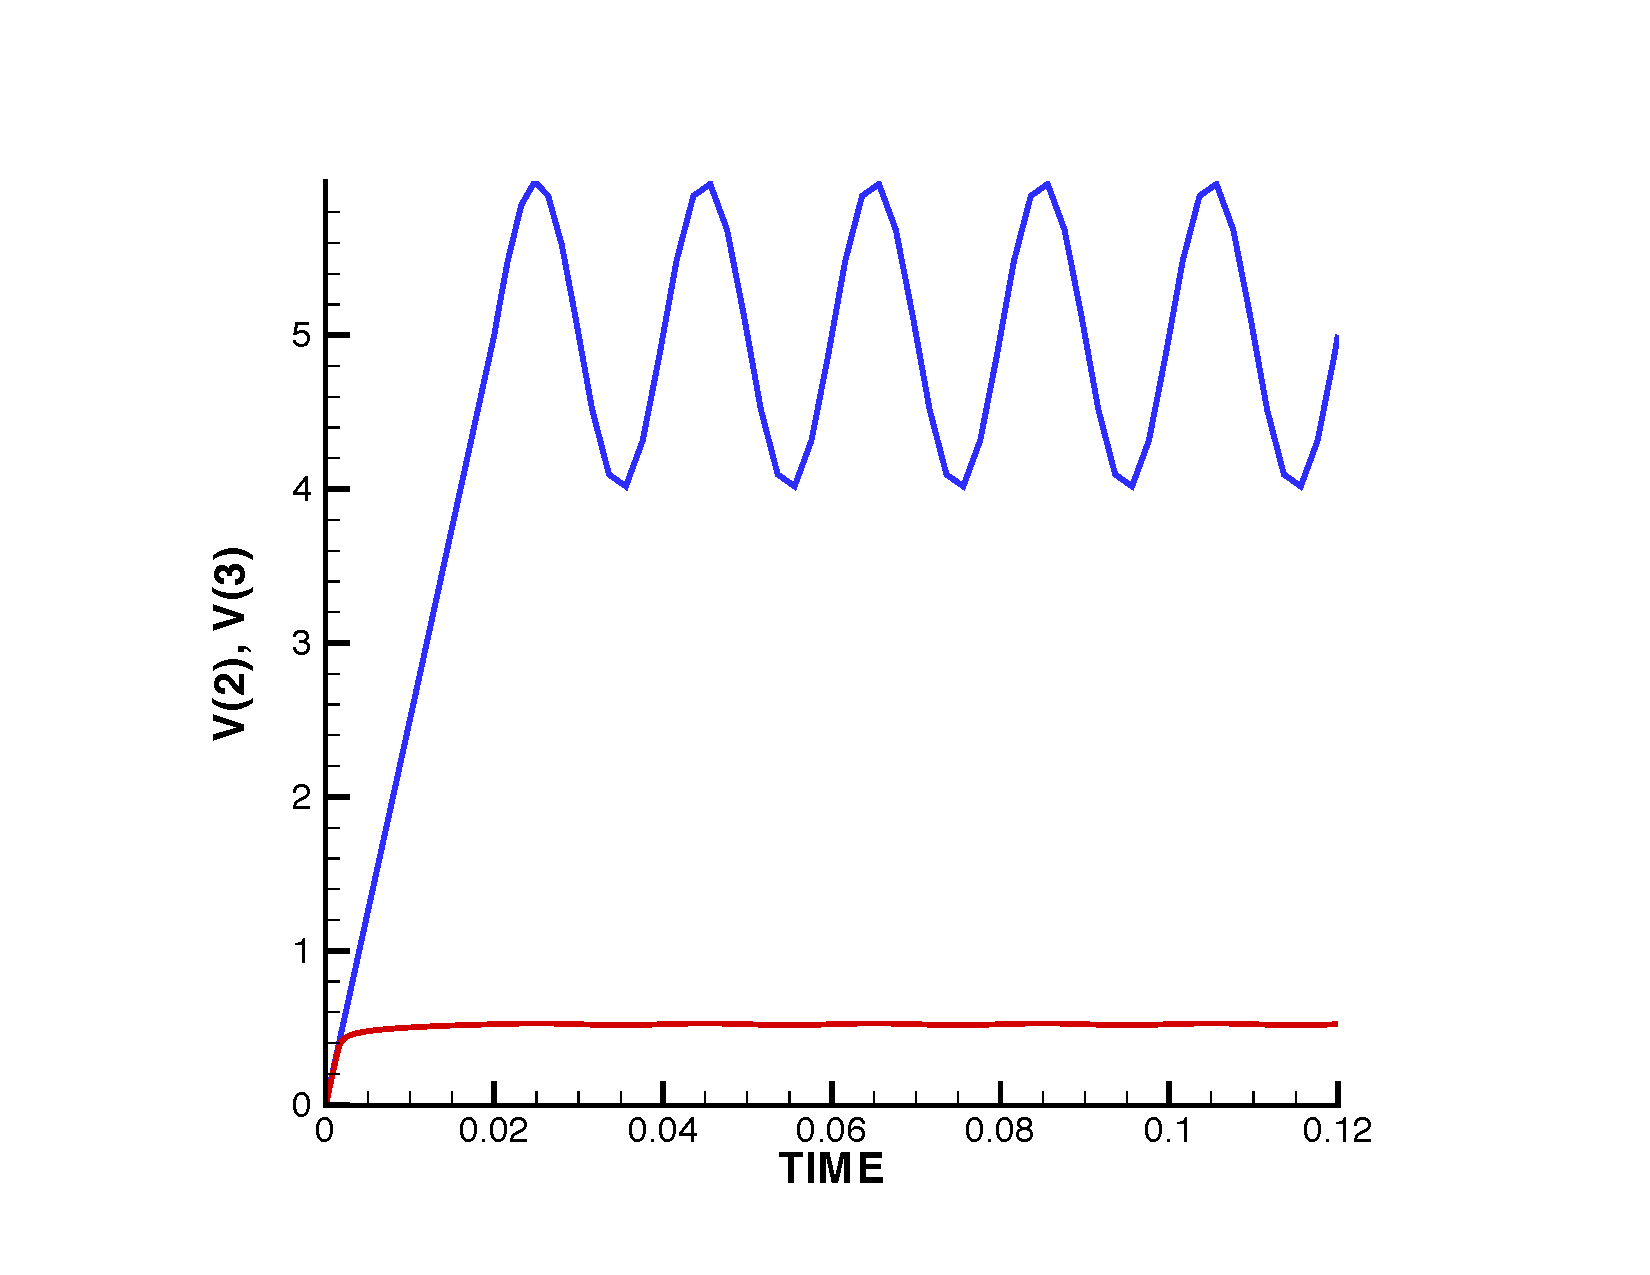
\includegraphics[scale=0.4]{Z1_trans}
\end{minipage}
\hspace{0.5cm}
\begin{minipage}[b]{0.5\linewidth}
\centering
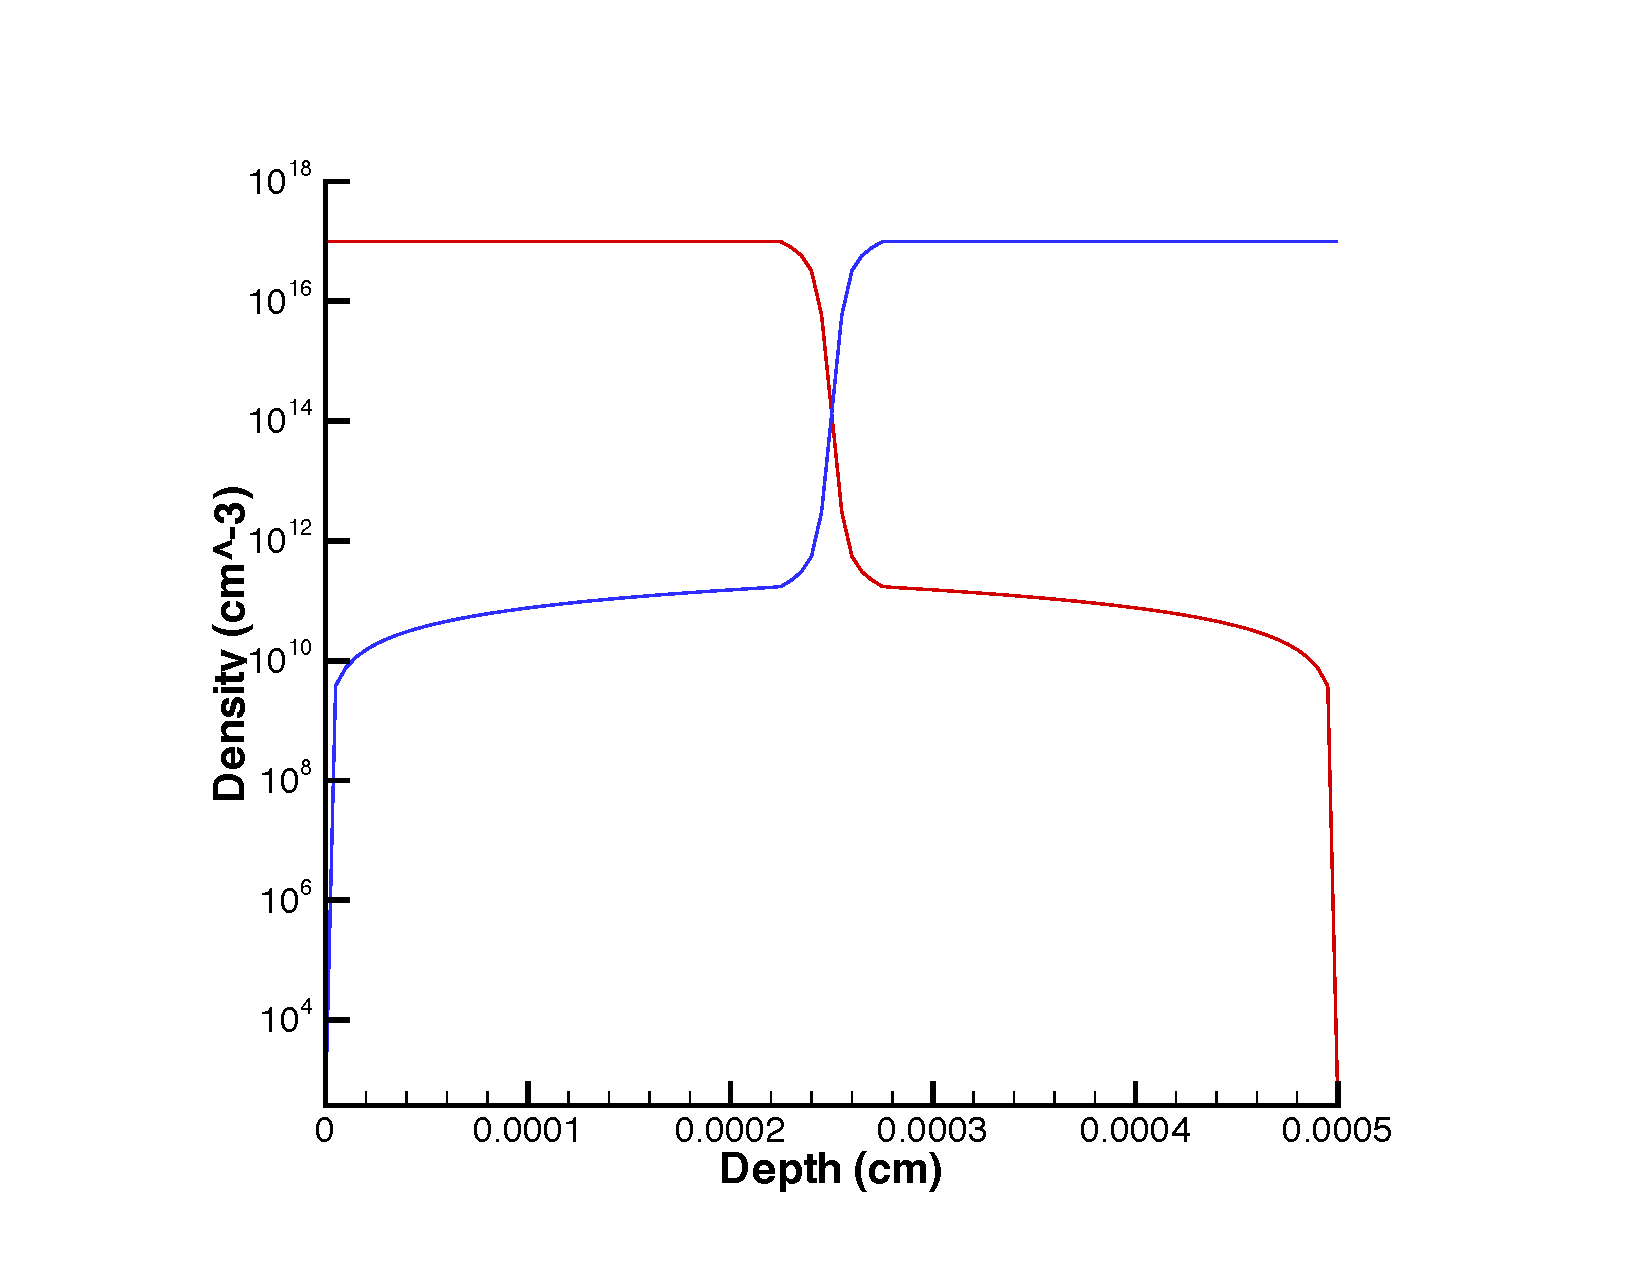
\includegraphics[scale=0.4]{Z1_dens}
\end{minipage}
\caption[Results for voltage regulator]{Results for voltage regulator.  In the left plot, the transient output is shown, in which the input voltage is blue and the output voltage is red.  In the right plot, the initial carrier densities are shown, with the electron density in red and the hole density in blue.}
\label{One_D_outputSignal}
\end{figure}

\section{Two-Dimensional Example} \label{PDE_Two_D_Example}
Figure~\ref{Two_D_BJT_Netlist} presents an example netlist for a simulation of 
a two-dimensional bipolar transistor.   As before, the PDE device instance line 
is in red, while the PDE device model line is in blue.  In this case, note that 
the model line specifies the level, which is set to 2.  This is required for the 
two-dimensional device.  This particular example is a DC sweep of a bipolar 
transistor device. Figure~\ref{twoD_BJT_Schem} presents a schematic illustrating 
this circuit.
% two dimensional netlist example
\begin{figure}
  \begin{centering}
    \shadowbox{
      \begin{minipage}{0.8\textwidth}
        \begin{vquote}
Two-Dimensional Example
VPOS  1 0 DC 5V
VBB   6 0 DC -2V
RE    1 2 2K
RB    3 4 190K

\color{XyceRed} YPDE BJT 5 3 7 PDEBJT meshfile=internal.msh 
+ node = \{name = collector, base, emitter\}
+ tecplotlevel=2 txtdatalevel=1
+ mobmodel=arora
+ l=2.0e-3  w=1.0e-3
+ nx=30     ny=15 
\color{XyceDarkBlue}.MODEL PDEBJT   ZOD  level=2 \color{black}

* Zero-volt sources acting as an ammeter to measure the
* base, collector, and emmitter currents, respectively
VMON1 4 6 0
VMON2 5 0 0
VMON3 2 7 0 

.DC VPOS 0.0 12.0 0.5 VBB -2.0 -2.0 1.0
.options NONLIN maxstep=70 maxsearchstep=1 
+ searchmethod=2 
.options TIMEINT reltol=1.0e-3 abstol=1.0e-6 
+ firstdcopstep=0 lastdcopstep=1
.PRINT DC V(1) I(VMON1) I(VMON2) I(VMON3)
.END
\end{vquote}

\end{minipage}
}
\caption[Two-dimensional BJT netlist]
{Two-dimensional BJT netlist.  Figures~\ref{twoD_BJTResA} and~\ref{twoD_BJTResB} provide some of the results of this netlist.\label{Two_D_BJT_Netlist}}
\end{centering}
\end{figure}
% BJT Circuit Schematic
% Original dimensions of picture: w=5.62 h=7.35 (inches)
\begin{figure}
  \centering
  \scalebox{0.5}
  {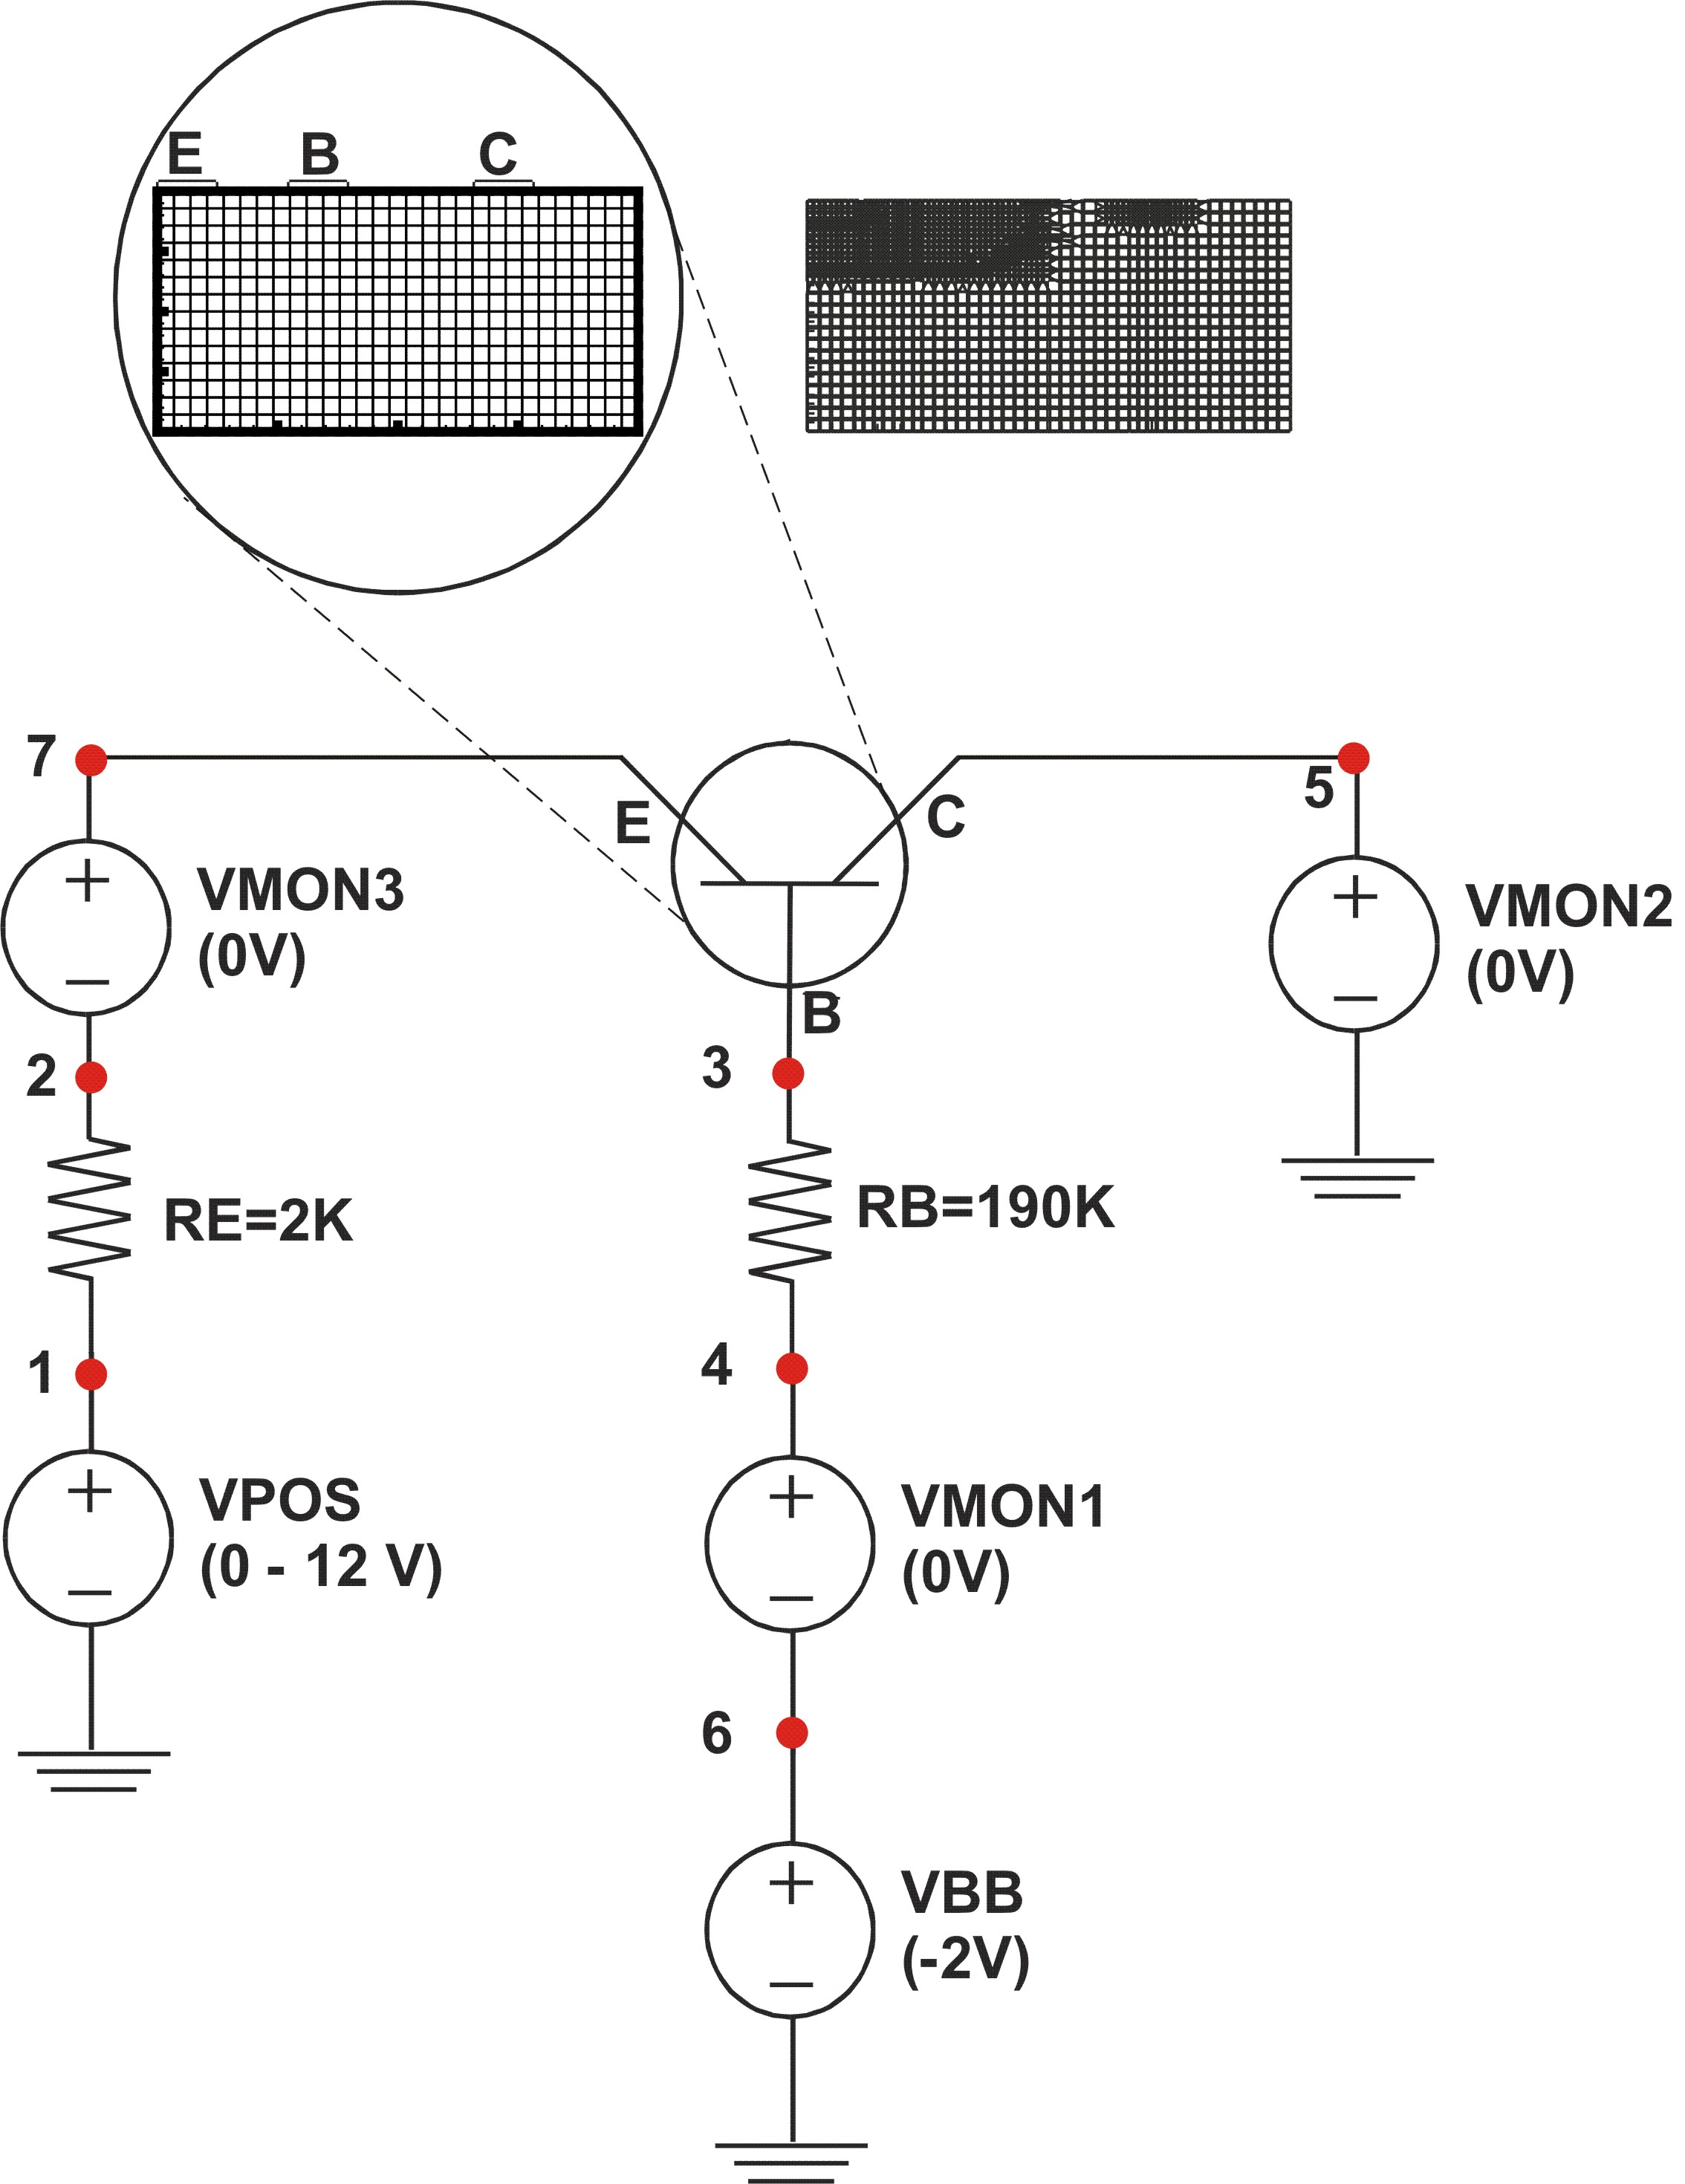
\includegraphics[]{twoDcircuit}}
  \caption[Two-dimensional BJT circuit schematic]
  {Two-dimensional BJT circuit schematic This schematic is for the circuit described by the netlist in figure~\ref{Two_D_BJT_Netlist}.  The mesh in the large circle is the mesh used in the example.  The other mesh, which contains some mesh refinement, is included in the figure as an example of what is possible with an external mesh generator.
\label{twoD_BJT_Schem}}
\end{figure}

\subsection{Netlist Explanation}
The two-dimensional device can have 2 to 4 electrodes.  In this example there
are three; nodes 5, 3, and 7, corresponding to the three names
on the ``node'' line,  which appears as:

\texttt{+ node = \{name = collector, base, emitter\} }

This line specifies that node 5 is connected to an electrode named 
``collector,'' node 3 is connected to an electrode named ``base,'' and node 7
is connected to an electrode named ``emitter''.    Although this example only
contains the electrode names, the ``node'' specification
can contain a lot of information. Section~\ref{PDE_Electrode} provides a full explanation of the
electrode parameters.  

The next line contains parameters concerned with plotting the results, and
appears as follows:

\texttt{+ tecplotlevel=2 txtdatalevel=1}

These are not related to the output specified by \texttt{.PRINT}, which outputs circuit data.  
The \texttt{tecplotlevel} command enables files to be output readable by Tecplot,  
which can then be used to create contour plots of 
quantities such as the electron density, electrostatic potential and the
doping profile.  Figures~\ref{twoD_BJTResA} and~\ref{twoD_BJTResB} 
contain examples of Tecplot-generated contour plots, which were generated
from the results of this example.

The \texttt{txtdatalevel} command enables a text file with volume averaged
information to be output to a file.  \Xyce{} will update both of 
these output files at each time step or DC sweep step.

The next line, \texttt{mobmodel=arora}, specifies which mobility model to
use.  Section~\ref{PDE_Mobility} provides for more detail on available mobility models.

The last two lines, specify the mesh of the device, and are given by:

\texttt{+ l=2.0e-3  w=1.0e-3} \\
\texttt{+ nx=30     ny=15}

This numbers are used in nearly the same way as the one-dimensional case used the \texttt{l} and
\texttt{nx} parameters.  The mesh is Cartesian, and the spacing is uniform.  

\subsection{Doping Profile}
As in the one-dimensional example, the two-dimensional example in figure
~\ref{Two_D_BJT_Netlist} specifies nothing about the doping profile, and thus 
relies on default settings.  In this case there are three specified electrodes, 
which by default results in the doping profile of the bipolar junction transistor (BJT).  
Section~\ref{PDE_Doping} provides a complete description of how to specify a 
doping profile, and describes the various default impurity profiles.

\subsection{Boundary Conditions and Electrode Configuration}
As in the one-dimensional example, the two-dimensional example in
figure~\ref{Two_D_BJT_Netlist} specifies nothing about
the electrode configuration or the boundary conditions, and relies on
default settings.  To be consistent with the default three-terminal doping,
the device has terminals that correspond to that of a BJT.  All three
electrodes (collector, base, emitter) are along the top of the device.

By default all electrodes are considered to be neutral contacts.  The 
boundary conditions applied to the electron density, hole density, and 
electrostatic potential are all Dirichlet conditions.

Section~\ref{PDE_Electrode} discusses how to specify electrodes in detail 
(including boundary conditions).

\subsection{Results}
Figures~\ref{twoD_BJTResA}, ~\ref{twoD_BJTResB} and ~\ref{twoD_BJTResC} provide 
results for the two-dimensional example.  The first two figures are contour plots 
of the electrostatic potential.  The first corresponds to the first DC sweep step, 
where VPOS is set to 0.0 Volts.  The second corresponds to the final DC sweep 
step, in which VPOS has a value of 12.0 volts.  The voltage source, VPOS, 
applies a voltage to the emitter load resistor, RE, so some of the 12.0V is 
dropped across RE, an the rest is applied to the BJT.

The third figure is an I-V curve of the dependence of the three terminal currents 
on the applied emitter voltage.  For the entire sweep, $-2.0$ V has been applied to 
the base load resistor and, as this transistor is a PNP transistor, this results 
in the transistor being in an ``on'' state.  The emitter-collector current varies 
nearly linearly with the applied emitter voltage. Also, as can be expected 
because of current conservation, the three currents sum to nearly zero.

Note that the mesh used to generate these results is visible in 
figure~\ref{twoD_BJTResA}, and was generated using the internal ``uniform mesh''.  
This mesh will not produce a very accurate result, as it does not 
resolve the depletion regions very well.  Accuracy can often be improved 
using mesh refinement near the depletion regions.  However, such meshes must be 
read in from an external mesh generator, which currently has limited support
as a alpha-level capability.

% BJT steady state, initial step.
\begin{figure}
  \centering
  \scalebox{1.0}
  {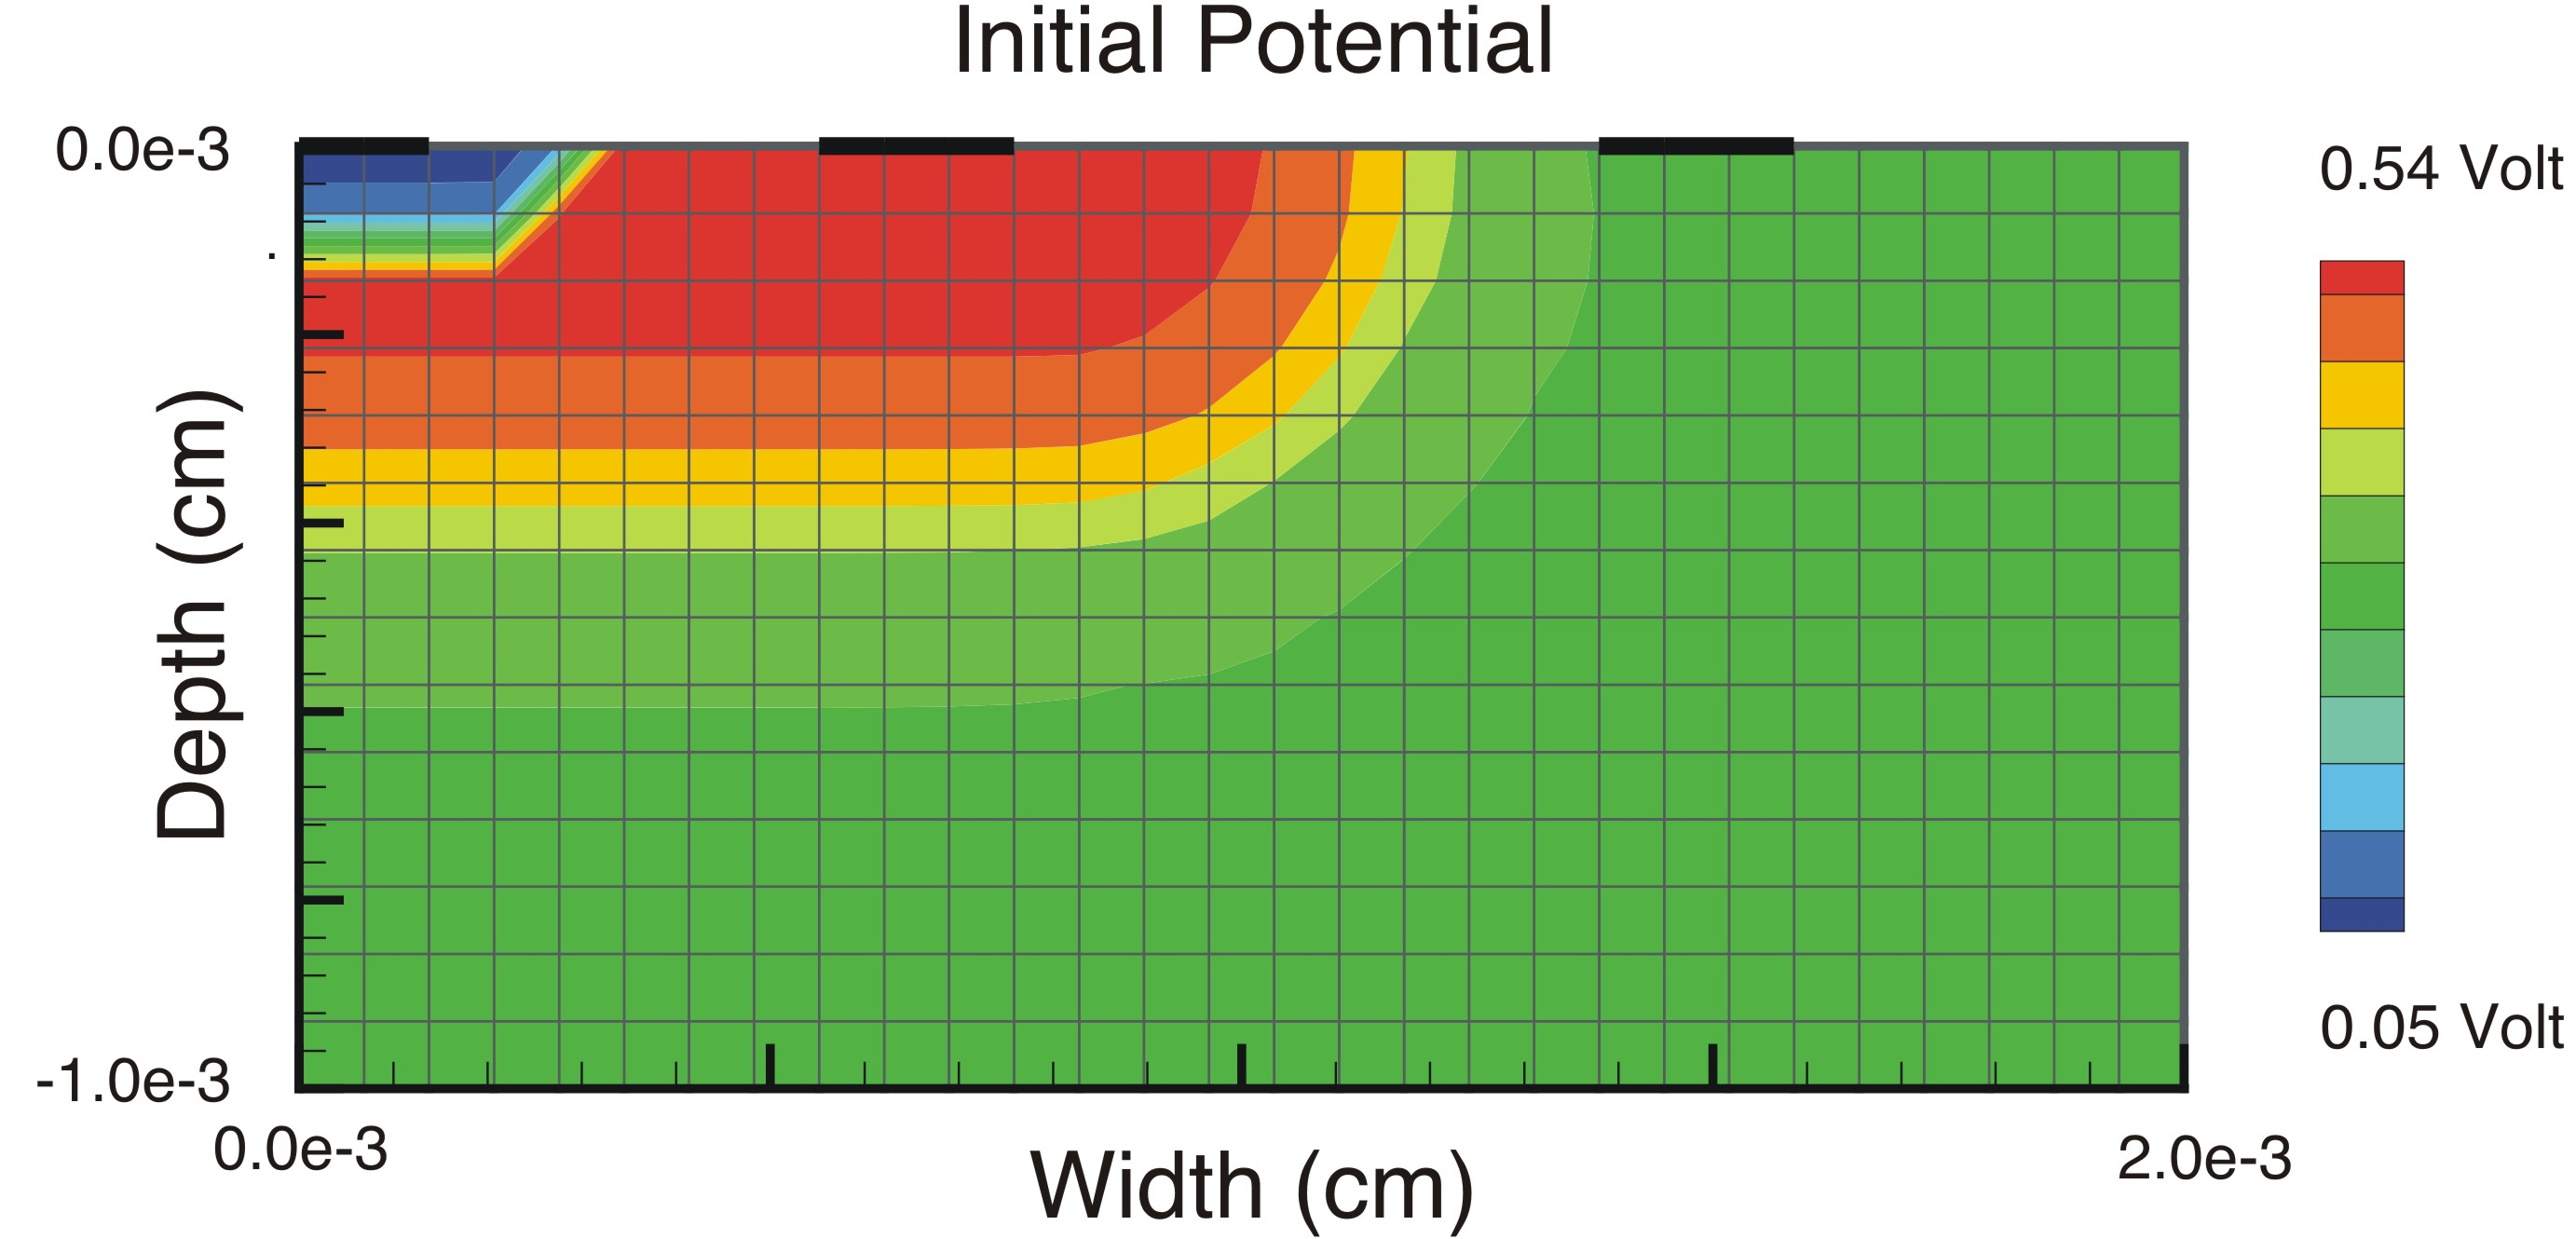
\includegraphics[width=4.610in,height= 2.165in]{twoDresultA}}
  \caption[Initial two-dimensional BJT result]
  {Initial two-dimensional BJT result
A Tecplot-generated contour plot of the electrostatic potential at the first DC 
  sweep step of the netlist in figure~\ref{Two_D_BJT_Netlist}.  
\label{twoD_BJTResA}}
\end{figure}

% BJT steady state, final step.
\begin{figure}
  \centering
  \scalebox{1.0}
  {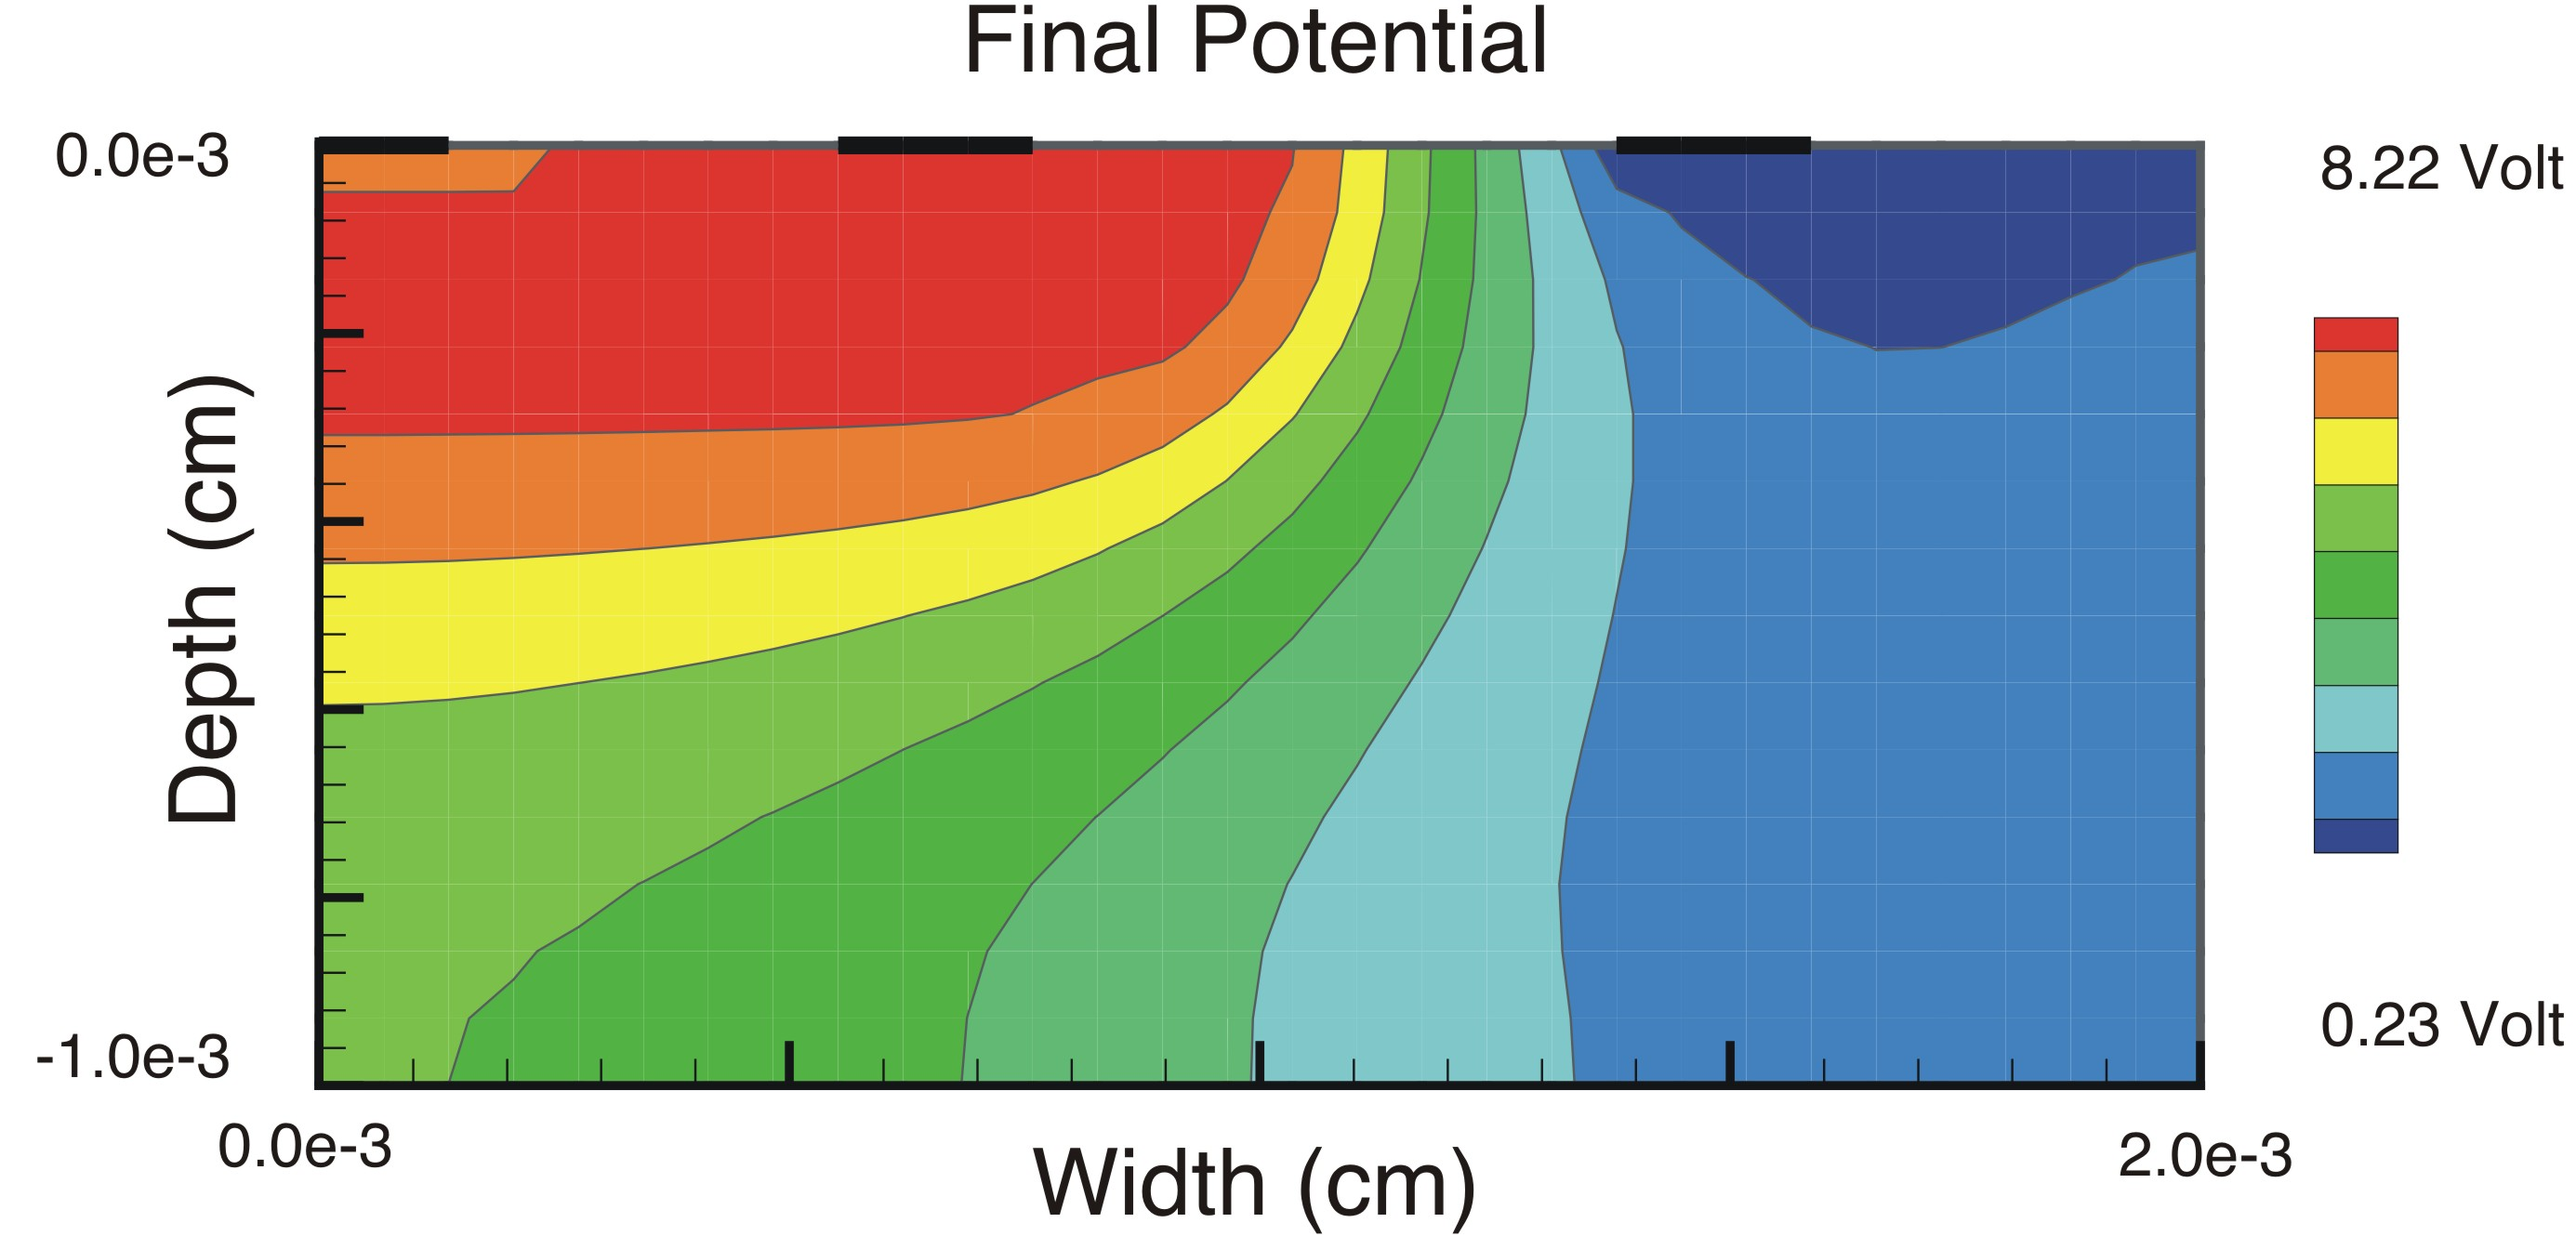
\includegraphics[width=4.610in,height= 2.165in]{twoDresultB}}
  \caption[Final two-dimensional BJT result.]
  {Final two-dimensional BJT result.  
A Tecplot-generated contour plot of the electrostatic potential at the last DC sweep 
  step of the netlist in figure~\ref{Two_D_BJT_Netlist}.  
\label{twoD_BJTResB}}
\end{figure}

% BJT steady state, I-V curve.
\begin{figure}
  \centering
  \scalebox{0.5}
  {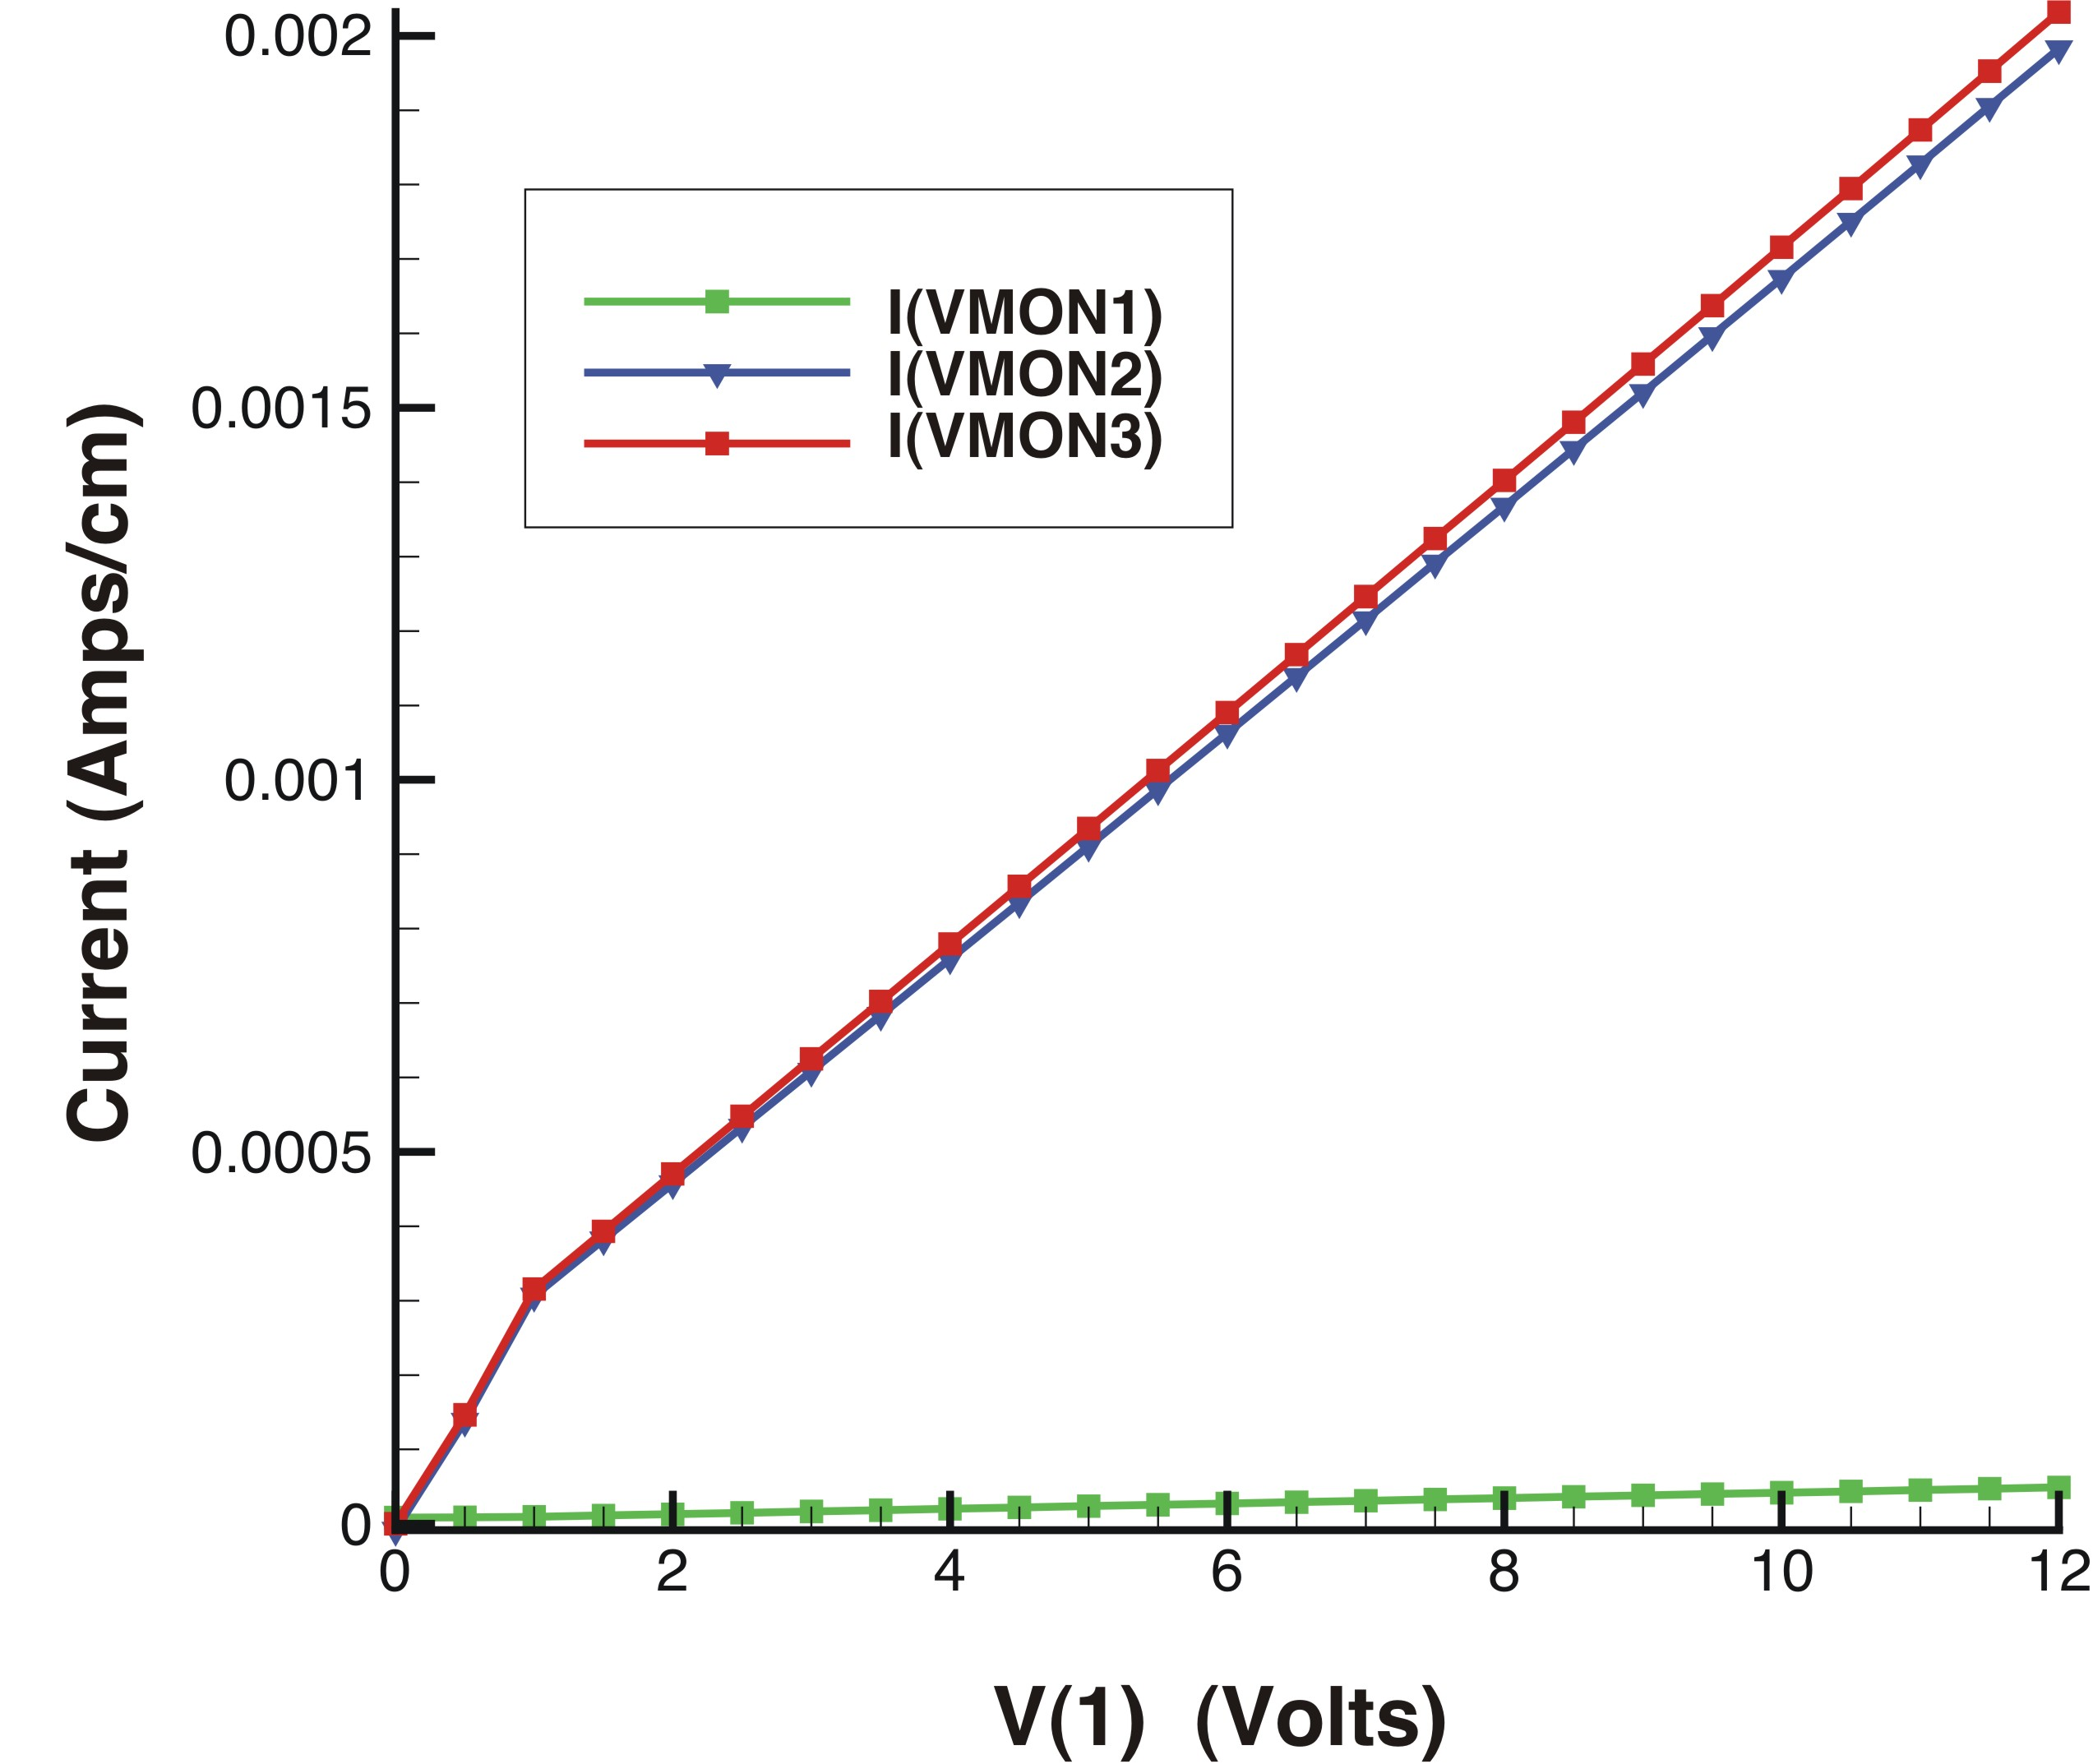
\includegraphics[]{twoDresultC}}
  \caption[I-V two-dimensional BJT result for the netlist in figure~\ref{Two_D_BJT_Netlist}]
  {I-V two-dimensional BJT result for the netlist in figure~\ref{Two_D_BJT_Netlist}.  
The three plotted currents are through the three BJT electrodes, and as expected they add (if corrected for sign) to zero.  I(VMON1) is the base current, I(VMON2) the collector current, and I(VMON3) the emitter current.  V(1) is the voltage applied to the emitter load resistor, RE.  
\label{twoD_BJTResC}}
\end{figure}

\section{Doping Profile} \label{PDE_Doping}
\Xyce{} used default doping profiles in the two examples from the previous section, so no doping parameters were 
specified.  Default profiles are uniquely specified by the number
of electrodes.  In practice, especially for two-dimensional simulations, the user will generally need to specify the doping profile manually.

\subsection{Manually Specifying the Doping} \label{Manual_Doping}
Figure~\ref{One_D_Doping_Electrode_1} shows a circuit netlist for a one-dimensional device with 
a detailed, manual specification of the doping
profile.  Figure~\ref{Two_D_Doping_Electrode_1} illustrates a similar, two-dimensional version of this problem. For this
discussion, the one-dimensional example will be referred to, but the information conveyed is equally applicable to the two-dimensional case.

In both examples, the parameters associated with doping are in red text.  The doping is specified with one or
more regions, which are summed together to obtain the total profile.  Doping regions are specified in a tabular format, with each column
representing a different region.  

\begin{figure}
  \begin{centering}
    \shadowbox{
      \begin{minipage}{0.8\textwidth}
        \begin{vquote}

\color[gray]{0.5}Doping and Electrode specification example
vscope   0   1   0.0
rscope   2   1   50.0
cid      3   0   1.0u
r1       4   3   1515.0
vid      4   0   5.00 \color{black}
YPDE Z1DIODE 2 3 PDEDIODE nx=301 l=26.0e-4 
\color{XyceRed}* DOPING REGIONS:    region 1,  region 2,   region 3
+ region= \{name     =    reg1,      reg2,  reg3
+          function = uniform,  gaussian,  gaussian
+          type     =   ntype,     ptype,     ntype
+          nmax     = 4.0e+12,   1.0e+19,   1.0e+18
+          nmin     = 0.0e+00,   4.0e+12,   4.0e+12
+          xloc     =    0.0 ,  24.5e-04,   9.0e-04
+          xwidth   =    0.0 ,   4.5e-04,   8.0e-04
+          flatx    =    0   ,        0 ,       -1 \}\color{black}
*--------end of  Diode PDE device ----------------\color[gray]{0.5}
.MODEL PDEDIODE  ZOD  level=1 
.options NONLIN maxsearchstep=1 searchmethod=2 
.options TIMEINT reltol=1.0e-3 abstol=1.0e-6 
.DC vscope 0 0 1
.print DC v(1) v(2) v(3) v(4) I(vscope) I(vid)
.END
\end{vquote}
\end{minipage}
}
\caption{One-dimensional example, with detailed doping
\label{One_D_Doping_Electrode_1}}
\end{centering}
\end{figure}

In the one-dimensional example, there are three regions, which are illustrated in
figure~\ref{Doping_Profile_1D}.  Region 1 is a uniform n-type
doping, with a constant magnitude of \texttt{4.0e+12} donors per cubic cm.  This 
magnitude is set by the parameter \texttt{nmax}.  As the
doping in this region is spatially uniform, the only meaningful parameters
are \texttt{function} (which in this case specifies a spatially uniform 
distribution), \texttt{type} (ntype or ptype) and \texttt{nmax}.  
The other parameters, \texttt{nmin} through \texttt{flatx} (1D) or \texttt{flaty} (2D), 
are ignored for a spatially uniform region.

Region 2 is a more complicated region, in that the doping profile varies
spatially.  This region is doped with p-type impurities, and the doping profile has a Gaussian
shape.  Semiconductor processing often consists of an implant followed by
an anneal, which results in a diffusive profile.  The Gaussian function 
is a solution to the diffusion problem, when it is assumed that the 
impurity exists in a fixed quantity.  

The peak of the Region 2 doping profile is given by the parameter \texttt{nmax}, 
and is \texttt{1.0e+19} acceptors per cubic cm. This peak has a location in the 
device specified by \texttt{xloc=24.5e-04 cm}.  The parameters \texttt{nmin} and 
\texttt{xwidth} are fitting parameters.

% Doping Profile
\begin{figure}
  \centering
  \scalebox{0.7}
  {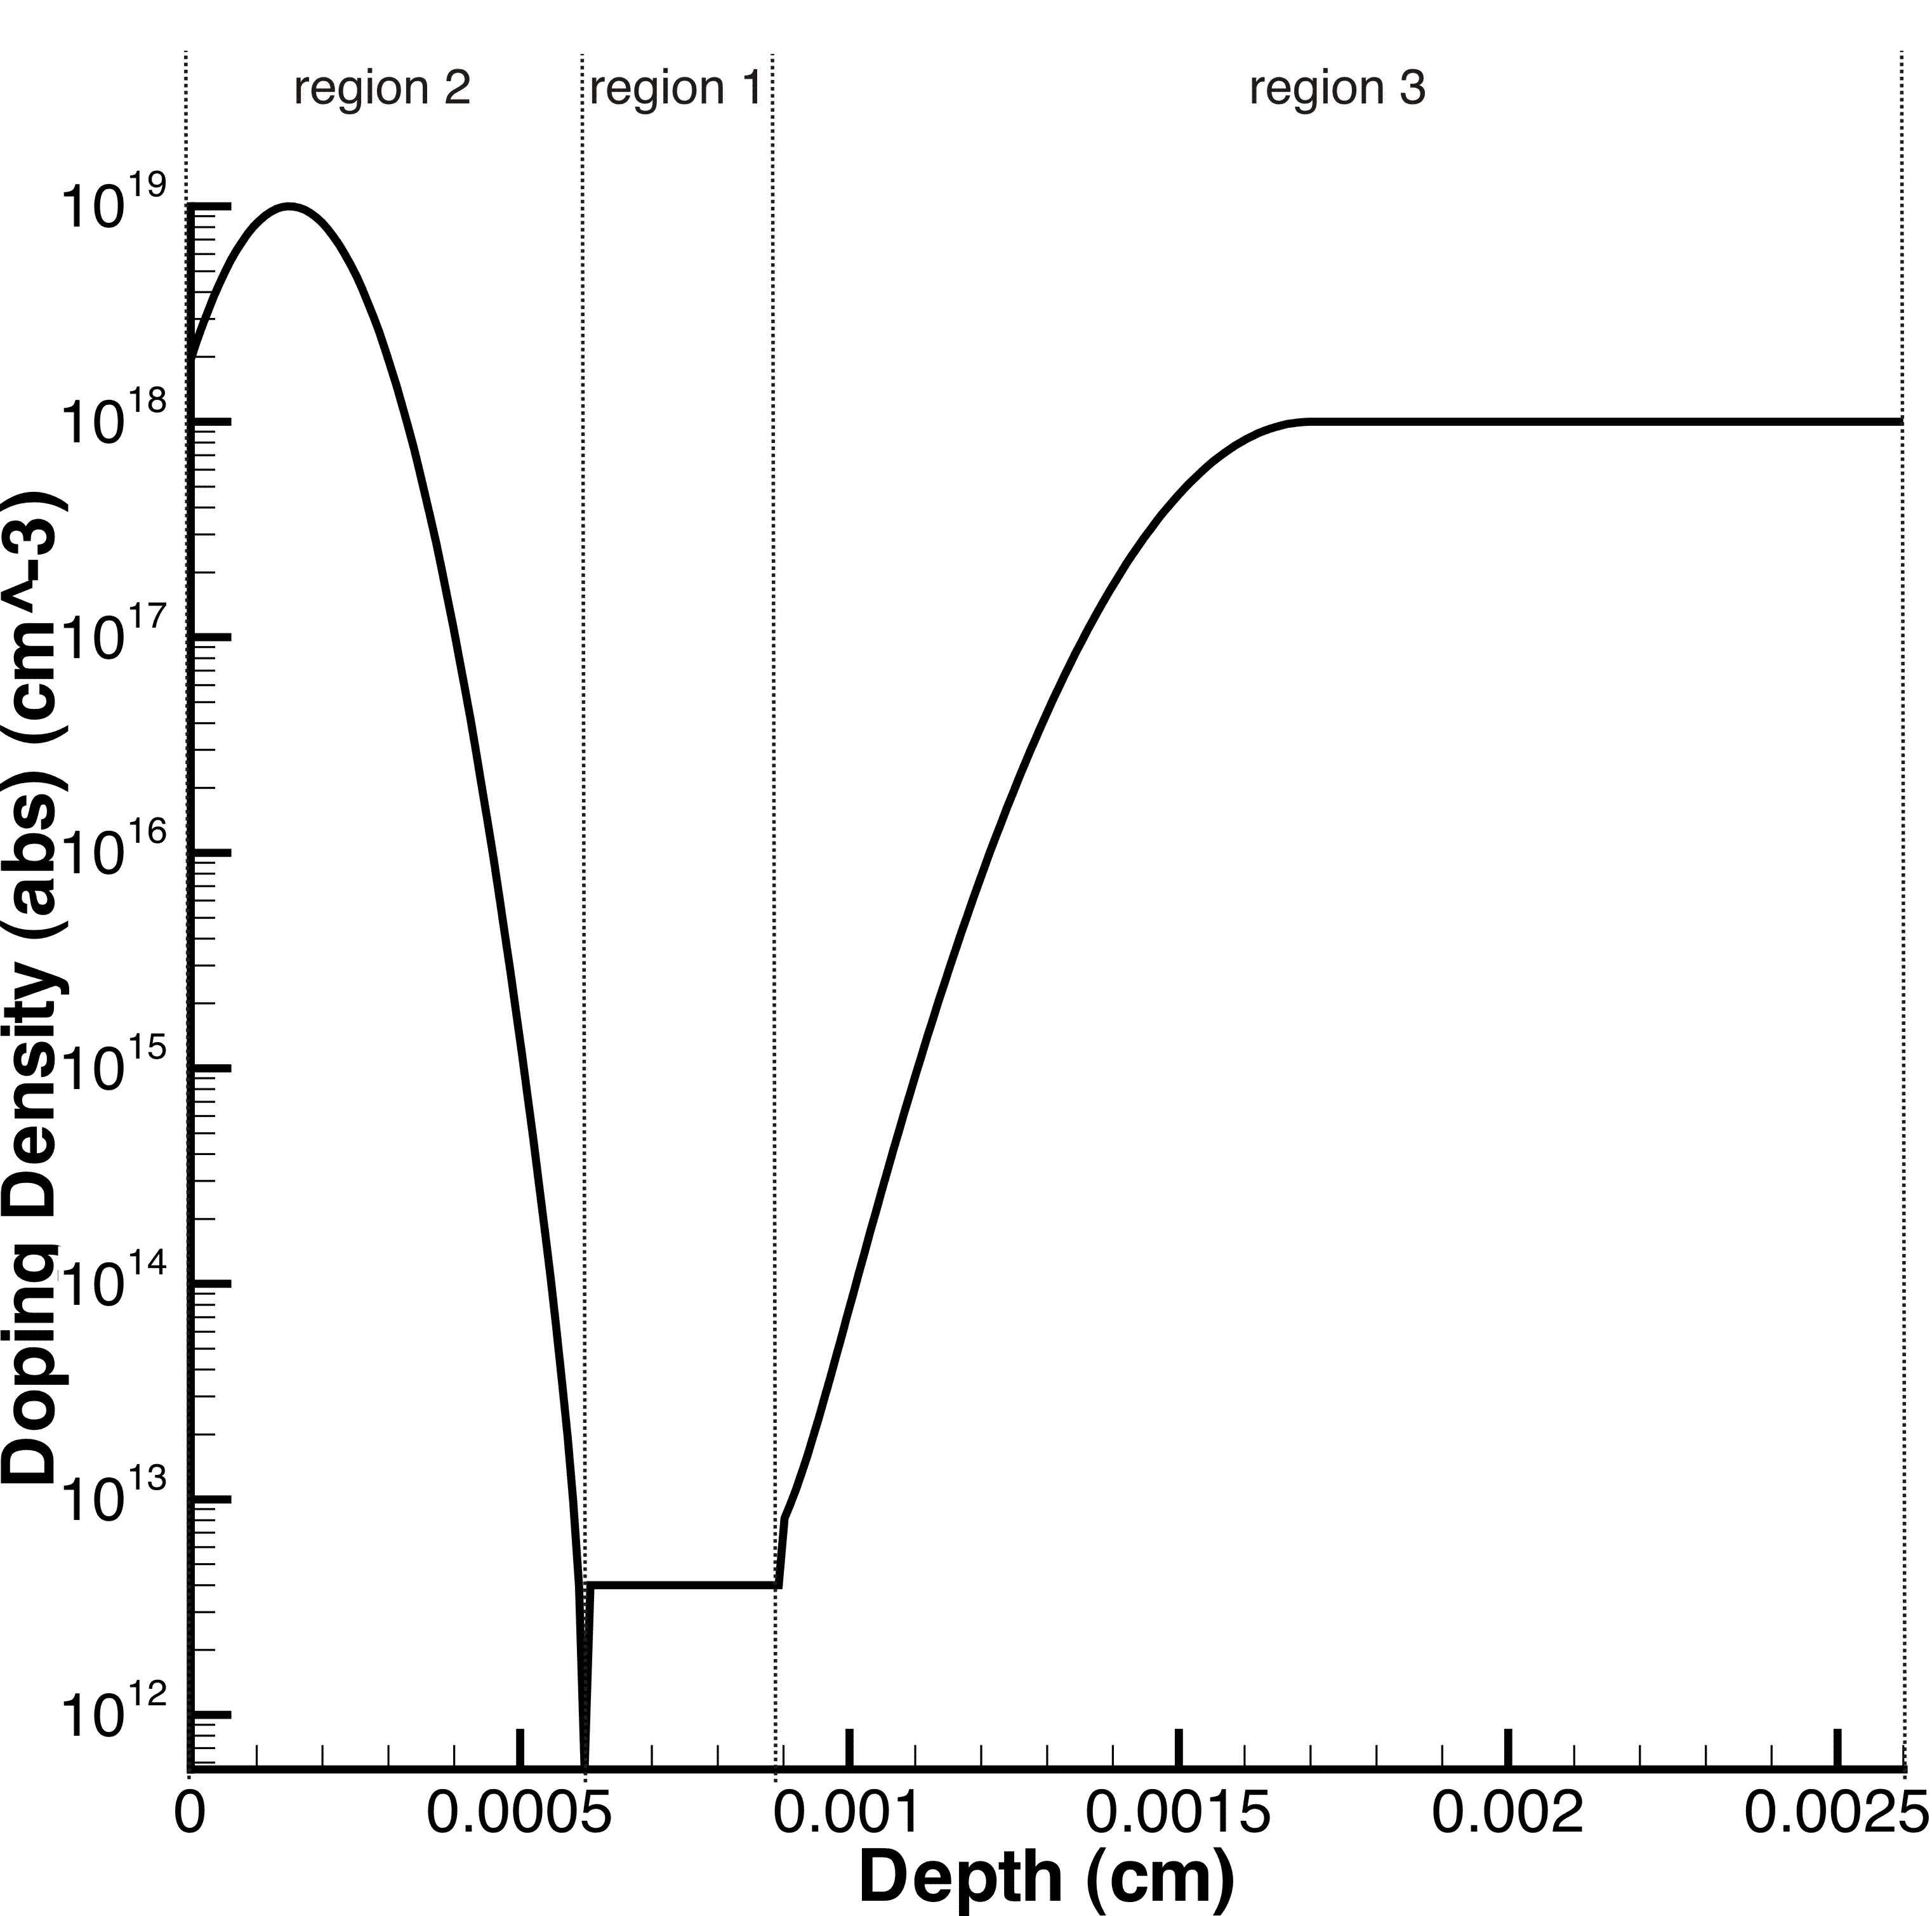
\includegraphics[width=4.610in,height= 4.45in]{doping_log}}
  \caption[Doping profile, absolute value]{Doping profile, absolute value  
This corresponds to the doping specified by the netlist in figure~\ref{One_D_Doping_Electrode_1}\label{Doping_Profile_1D}}
\end{figure}

Region 3 is also based on a Gaussian function, but unlike Region 2, it is 
flat on one side of the peak.  This is set by the \texttt{flatx} parameter.  
Table~\ref{flatxy_table} lists conventions for ``flat'' parameters.

\LTXtable{\textwidth}{flattbl}

\newpage
\subsubsection{Specifying doping profiles using expressions}
The \Xyce{} expression library can be used to specify doping profiles.  An example of this is given in 
figures~\ref{One_D_Doping_Electrode_Expression}.  In the example, the same \texttt{region} specification is 
used to specify doping regions.  However, unlike the previous example, each species is assigned an user-defined 
expression to define the profile as a function of depth.  This capability is only available for 
one dimensional devices.
\begin{figure}
  \begin{centering}
    \shadowbox{
      \begin{minipage}{0.8\textwidth}
        \begin{vquote}
\color[gray]{0.5}Expression doping example\color{black}
.param xs=1.0e+4\color{blue}; distance scalar\color{black}
.param A\_B=19.574867\color{blue};boron params\color{black}
.param x0\_B=-0.228
.param w\_B=0.152
.param A\_SB=18.61832\color{blue};antimony params\color{black}
.param x0\_SB=3.694
.param w\_SB=0.542
.param A\_AS=20.11501\color{blue};arsenic params\color{black}
.param x0\_AS=0.061
.param w\_AS=0.038
.Func ifmax (a,b) \{if(a>b, a, b)]\}
.Func FB(X)\{(10**A\_B)*exp(-((((X*xs)-x0\_B)/(2*w\_B))**2))\}
.Func FSB(X)\{(10**A\_SB)*exp(-((((X*xs)-x0\_SB)/(2*w\_SB))**2))\}
.Func FAS(X)\{(10**A\_AS)
+ *exp(-(((ifmax((X*xs)-x0\_AS,0))/(2*w\_AS))**2))\}
\color[gray]{0.5}V1 0 1 1.0
ypde diode  1 0 pdediode l=3.3e-5 nx=201 area=1.0 
\color{red}+ region={name       =          reg1,  reg2
+         function   =    expression,  expression
+         type       =         ptype,  ntype
+         expression =  \{FB(#x)\}, \{FAS(#x) + FSB(#x)\}
+         species    =            BM,  ASP }\color[gray]{0.5}
.MODEL pdediode  ZOD  level=1
.dc V1 1.0 1.0 1.0
.print dc v(1) {log10(abs(I(V1)))}
\end{vquote}
\end{minipage}
}
\caption{One-dimensional example, with expression-based doping.  
    Each of the functions 
    (FB, FAS and FSB) correspond to a different dopant, and are functions of depth.  The red text 
    shows where these three functions are used to specify doping profiles.
\label{One_D_Doping_Electrode_Expression}}
\end{centering}
\end{figure}

\newpage
\subsection{Default Doping Profiles}
\Xyce{} has a few default doping profiles that are invoked when the user
doesn't specify detailed doping information.  The default doping 
profiles are an artifact of early TCAD device development in \Xyce{}, but are 
sometimes still useful.  In particular, the simple step-junction diode
is often a useful canonical problem.  It is convenient to invoke a
step-junction doping without having to use the tabular specification
for more complex regions.

Most real devices will have doping profiles that do not exactly match the
default profiles.  When attempting to simulate a realistic device, it
will be necessary to skip the defaults and use the region tables described in
the previous section.

\subsubsection{One-Dimensional Case} \label{one_d_default_dope}
For the one-dimensional case, \Xyce{} assumes that the doping profile is a
simple junction diode, with the junction location exactly in the middle.  The
acceptor and donor concentrations are given by the parameters \texttt{Na} and
\texttt{Nd}, respectively.  

The use of ~\texttt{Na} and \texttt{Nd}, implicitly specifies a step junction
doping profile, and is mutually exclusive with the more complex ``doping
region'' table specification, described in section~\ref{Manual_Doping}.  If a
netlist is input to \Xyce{} with a ``doping region'' table and \texttt{Na} (or
\texttt{Nd}), the code will immediately exit with an error.

\subsubsection{Two-Dimensional Case} \label{two_d_default_dope}
Doping level defaults in the two-dimensional case are somewhat more complicated
than in the one-dimensional case, because having two-dimensions allows for more
configurations, and an arbitrary number (2 to 4) of electrodes.  During \Xyce{}
development, it was decided that the default doping profiles would be
determined uniquely by the number of electrodes present.
Table~\ref{Default_Doping_2D} provides the three available default dopings.  In
the case of the BJT and MOSFET dopings, it is possible to specify either n-type
or p-type using the \texttt{type} instance parameter.   If the detailed, manual
doping is used, then the \texttt{type} parameter is ignored.

For a two-electrode device, the default doping is that of a simple diode.
\Xyce{} uses the acceptor and donor doping parameters, \texttt{Na} and
\texttt{Nd}, in the same manner as in the one-dimensional device---the junction
is assumed to be exactly in the middle of the domain.

For a three-electrode device (as shown in the example), the default doping is
that of a bipolar junction transistor (BJT).  By default the transistor is a
PNP, but by setting the instance parameter \texttt{type=NPN}, an NPN transistor
can be specified instead.  The two-dimensional example in
section~\ref{PDE_Two_D_Example} relies on this default.  

For a four-terminal device, the default doping is that of a
metal-oxide-semiconductor (MOSFET).  The maximum number of electrodes is four,
and no default profiles are available for more than four electrodes.  By
default this transistor is assumed to be NMOS, rather than PMOS.

\LTXtable{\textwidth}{defdopingtbl}

\clearpage
\section{Electrodes} \label{PDE_Electrode}
Because minimal electrodes were specified in the two examples given above, \Xyce{}
used the defaults.  In practice, especially for two-dimensional simulations, the 
user must specify the electrodes in more detail.

% electrode specification example.  
\begin{figure}
  \begin{centering}
    \shadowbox{
      \begin{minipage}{0.8\textwidth}
        \begin{vquote}

\color[gray]{0.5}Doping and electrode specification example
vscope   1   0   0.0
rscope   2   1   50.0
cid      3   0   1.0u
r1       4   3   1515.0
vid      4   0   1.00 \color{black}
*------------- Diode PDE device ------------------
YPDE Z1DIODE 2 3 PDEDIODE
+ tecplotlevel=1 txtdatalevel=1 cyl=1
+ meshfile=internal.msh 
+ nx=25  l=70.0e-4 ny=40  w=26.0e-4 
\color{XyceDarkBlue} * ELECTRODES:             ckt node 2, ckt node 3
+ node = \{name           =     anode,    cathode
+         bc             = dirichlet,  dirichlet
+         start          =     0.002, 0.002
+         end            =     0.005, 0.005
+         side           =       top,     bottom
+         material       =   neutral,    neutral
+         oxideBndryFlag =         0,          0 \}
\color{XyceRed}* DOPING REGIONS:    region 1,  region 2,   region 3
+ region= \{name    =     reg1,      reg2,  reg3
+          function = uniform,  gaussian, gaussian
+          type     =   ntype,     ptype,     ntype
+          nmax     = 4.0e+12,   1.0e+19,   1.0e+18
+          nmin     = 0.0e+00,   4.0e+12,   4.0e+12
+          xloc     =    0.0 ,  60.0e-04,    100.0 
+          xwidth   =    0.0 ,   4.0e-04,      1.0 
+          yloc     =    0.0 ,  24.5e-04,   9.0e-04
+          ywidth   =    0.0 ,   4.5e-04,   8.0e-04
+          flatx    =    0   ,       -1 ,       -1 
+          flaty    =    0   ,        0 ,       -1 \}\color{black}
*--------end of  Diode PDE device ----------------\color[gray]{0.5}
.MODEL PDEDIODE  ZOD  level=2 
.options NONLIN maxsearchstep=1 searchmethod=2 
.options TIMEINT reltol=1.0e-3 abstol=1.0e-6 
.DC vscope 0 0 1
.print DC v(1) v(2) v(3) v(4) I(vscope) I(vid)
.END
\end{vquote}
\end{minipage}
}
\caption{Two-dimensional example, with detailed doping and detailed electrodes.
\label{Two_D_Doping_Electrode_1}}
\end{centering}
\end{figure}

\subsection{Electrode Specification}
A detailed electrode specification is specified in blue text
in figure~\ref{Two_D_Doping_Electrode_1}.  As with the doping parameters, 
the electrode parameters are specified in a tabular format, in which each table 
column specifies the different electrode parameters.  The \texttt{name} parameter 
is the only required parameter.

The number of specified electrodes must match the number of connected 
circuit nodes, and the order of the electrode columns, from left to right,
is in the same order as the circuit nodes, also from left to right.  In 
the figure~\ref{Two_D_Doping_Electrode_1} example, the first electrode column,
which specifies an electrode named ``anode,'' is connected to the circuit 
through circuit node 2.  Respectively, the second column, for the ``cathode'' 
electrode, is connected to the circuit via circuit node 3.

\subsubsection{Boundary Conditions}
In the example, the default \texttt{bc} parameter has been set to ``Dirichlet''
on all the electrodes. The \texttt{bc} parameter sets the type of boundary 
condition applied to the density variables, the electron density and the hole density.
Dirichlet and Neumann are two possible settings for the \texttt{bc} parameter.  
If Dirichlet is specified, the electron and hole densities are set to a specific 
value at the contact, and the applied values enforce charge neutrality.  
(Note: The \Xyce{} Reference Guide\ReferenceGuide{} provides the charge-neutral 
equation.)  If Neumann is specified, \Xyce{} applies a zero-flux condition, 
which enforces that the current through the electrode will be zero.

This parameter does not affect the electrostatic potential boundary condition.
The boundary condition applied to the potential is always Dirichlet, and is
(in part) determined from the connected nodal voltage.  To apply a specific
voltage to an electrode contact, a voltage source should be attached to it,
such as \texttt{VBB} in figure~\ref{twoD_BJT_Schem}.

\subsubsection{Electrode Material}
Table~\ref{contactMaterialTable} lists several different electrode materials that can be specified.   
The main effect of any metal (nonneutral) material is that \Xyce{} imposes a
Schottky barrier at the contact, generally making numerical solutions
more difficult, so materials should be applied with caution.

The \Xyce{} Reference Guide\ReferenceGuide{}
provides a detailed description of Schottky barriers and how they are imposed on contacts in \Xyce{}.
The guide also provides values for electron affinities of various bulk materials and 
workfunction values for the various metal contacts.

\LTXtable{\textwidth}{contactMaterialtbl}

There is also an \texttt{oxideBndryFlag} parameter, which if set to true
(\texttt{1}), will model the contact as having an oxide layer in between
the metal contact and the bulk semiconductor.  By default,
\texttt{oxideBndryFlag} is false (\texttt{0}).  

\subsubsection{Location Parameters}
Each electrode has three location parameters: \texttt{start}, 
\texttt{end}, and \texttt{side}.  

\Xyce{} assumes the internal mesh to be rectangular, 
and the electrodes can be on any of the sides.  The four side possibilities
are: \texttt{top}, \texttt{bottom}, \texttt{right} and \texttt{left}.
These four sides are parallel to the mesh directions.  The \texttt{start} and
\texttt{end} parameters are floating-point numbers that specify the
starting and ending location of an electrode, in centimeters.

The lower left hand corner of the mesh rectangle is located 
at the origin.  A \texttt{side=bottom} electrode with \texttt{start=0.0} 
and \texttt{end=1.0e-4} will originate at the lower left hand 
corner of the mesh (x=0.0, y=0.0) and end at (x=1.0e-4, y=0.0).

\Xyce{} will attempt to match the specified electrode to
the specified mesh.  However, if the user specifies a mesh that is not
consistent with the electrode locations then the electrodes will not be 
able to have the exact length specified.  For example, if the mesh spacing
is $\Delta x = $ 1.0e-5, then the electrodes can only have a length
that is a multiple of 1.0e-5.

\subsection{Electrode Defaults}
Defaults exist for each electrode parameter other than names.
In practice, the electrode locations  are usually explicitly
specified  using the electrode table.
Default electrode locations were created to correspond with 
the default dopings; they should only be used in that context.

\subsubsection{Location Parameters}
In practice, the electrode locations will usually be explicitly
specified, but they have defaults to correspond with the default dopings.
The default electrode locations in one-dimensional devices are for a 
diode.  One electrode is located at \texttt{x=xmin}, while the other 
is located at \texttt{x=xmax}.

The default electrode locations in two-dimensional devices depend on the number 
of electrodes, similar to the default dopings.  Table~\ref{Default_Doping_2D} can be 
used to determine such configurations.  For the two-terminal diode, 
the two electrodes are along the  y-axis, at the \texttt{x=xmin} and 
\texttt{x=xmax} extrema.
For the three-terminal BJT, all three electrodes are parallel to the
x-axis, along the top, at \texttt{y=ymax}.  For the four-terminal MOSFET, the 
drain, gate, and source electrodes are also along the top, but the bulk 
electrode spans the entire length of the bottom of the mesh, at 
\texttt{y=ymin}.

\section{Meshes} \label{PDE_Mesh}
One- and two-dimensional devices can create Cartesian meshes.
For two-dimensional devices, users must specify \texttt{meshfile=internal.msh} 
to invoke the Cartesian meshing capability (this is necessary for historical reasons).
Meshes generated in this manner are very simple as there are only two
parameters per dimension, and the resulting mesh is uniform.  Figure~\ref{twoD_BJTResA} 
provides an example of such a mesh.  Mesh spacing is determined from the following expressions:
\begin{eqnarray}
  \Delta x = \frac{l}{nx-1}  \\
  \Delta y = \frac{w}{ny-1} 
\end{eqnarray}
This mesh specification assumes the domain is a rectangle.  
Nonrectangular domains can only be described using an external mesh program.

Externally generated meshes for 1D devices can be including using
\texttt{meshfile=<filename>} in the PDE device instance line. The file
specified by \texttt{<filename>} must consist of two space-delimited columns of
numbers. The first column specifies the location of the mesh points. The second
column is not currently used, but it must exist, so it is suggested to make it
a column of zeros.

\section{Cylindrical meshes}
For two-dimensional devices, the simulation area may be a cylinder slice.  
This capability is turned on by the instance parameter {\tt cyl=1} 
It is assumed that the
axis of the cylinder corresponds to the minimum radius (or x-axis value) of the 
mesh, while the circumference corresponds to the maximum radius (or maximum x-axis value).  

\section{Mobility Models}
\label{PDE_Mobility}
There are several mobility models available to the one- and two-dimensional 
devices, and they are listed in Table~\ref{Mobility_Models}.
These models are fairly common, and can be found in most device
simulators.~\cite{Yu}~\cite{DaVinci}. The \Xyce{} Reference 
Guide\ReferenceGuide{} descibes these models in more detail.

\LTXtable{\textwidth}{mobilitytbl}

Setting the {\texttt{mobmodel}} parameter to the name of the model (as provided 
in the first column of table~\ref{Mobility_Models}) specifies the mobility model 
from the netlist. The mobility model is specified as an instance parameter on the 
device instance line, as (typically) {\texttt {mobmodel=arora}}.
Figure~\ref{Two_D_BJT_Netlist} provides a more detailed 
example.

The default mobility is ``arora'', which is a basic model lacking carrier or field dependence.  
Because it lacks these dependencies, it generally is more numerically robust.  The ``carr'' model
include carrier-carrier dependence, as does the ``philips'' model.  For all of these models,
field dependence can be optionally turned on from the netlist, using the \texttt{fielddep=true} parameter.

\section{Bulk Materials}
\label{PDE_Bulk_Material}
The bulk material is specified using the \texttt{bulkmaterial} instance
parameter.  \Xyce{} supports Silicon (\texttt{si}) as a default bulk material.  
It can also simulate several III-V materials, including Gallium Arsenide (\texttt{gaas}), Germanium (\texttt{ge}), Indium Aluminum Arsenide (\texttt{inalas}  or \texttt{alinas}),
Indium Galium Arsenide (\texttt{ingaas} or \texttt{gainas}), Indium Phosphide(\texttt{inp}), and
Indium Galium Phosphide (\texttt{ingap}); but these materials have not been extensively tested.
The mobility models described in the previous section each support most of these materials.

\section{Output and Visualization}
\label{PDE_Output_Vis}

\subsection{Using the \texttt{.PRINT} Command }
For simple plots (such as I-V curves), output results for \Xyce{}
can be generated with the \texttt{.PRINT} statement, which is described in
detail in section~\ref{PRINT_section}.
Figures~\ref{One_D_outputSignal} and~\ref{twoD_BJTResC} are examples of
the kind of data that is produced with \texttt{.PRINT} statement
netlist commands.  These particular figures were plotted in Tecplot, but
many other plotting programs would also have worked, including
XDAMP~\cite{xdamp}.

\subsection{Multidimensional Plots}
Device simulation has visualization needs which go beyond that of 
conventional circuit simulation.  Multidimensional perspective and/or
contour plots are often desirable.  \Xyce{} is capable of outputting
multi-dimensional plot data in several formats, including Tecplot (available 
for purchase from http://www.tecplot.com), 
gnuplot (available free from http://www.gnuplot.info), and SGPLOT.
Currently, the options for each of these formats can only enable
or disable the output of files, and when enabled, a new file (or a new
append to an existing file) will happen at every time step or DC sweep
step.

For long simulations, this may produce a prohibitive number of files.  There is
no equivalent to the \texttt{.OPTIONS OUTPUT INITIAL\_INTERVAL} command, nor
does the output of plot data use this command.   Plot files are either output
at every step or not at all.

For each type of plot file, the file is placed in the execution directory.
Each individual device instance is given a unique file, or files, and
the file names are derived from the name of the PDE device instance.  The
instance names provides the prefix, and the file type (Tecplot,
gnuplot, Sgplot) determines the suffix.

\subsubsection{Tecplot Data}
Tecplot is a commercial plotting program from Amtec Engineering, Inc.,
and is a good choice for creating contour plots of spatially dependent
data.  All of the graphical examples in this chapter were created with
Tecplot. (See figures~\ref{twoD_BJTResA} and~\ref{twoD_BJTResB} for examples.)
The output of Tecplot files is enabled using the instance parameter,
\texttt{tecplotlevel=1}.  If set to zero, no Tecplot files are output.
If set to one, \Xyce{} outputs a separate Tecplot file for each nonlinear solve.
If set to two, \Xyce{} creates a single Tecplot file containing data for every 
nonlinear solve and appends the file at the end of each solve.

By default \texttt{tecplotlevel} is set to one, meaning the code will produce 
a separate Tecplot file for each time step or DC sweep step.   The
suffix for a Tecplot (ASCII text) data file is *.dat.

\subsubsection{Gnuplot Data}
Gnuplot is an open source plotting program available on most
Linux/Unix platforms.  The parameter for this type of output is 
\texttt{gnuplotlevel=1}.  This type of output file is off (zero) by 
default, meaning no gnuplot files will be output.  The suffix for gnuplot
files is *gnu.dat.  Like Tecplot files, gnuplot files are also in ASCII
text format.

\subsection{Additional Text Data}
\Xyce{} can also output additioanl information for each PDE device by setting 
the instance parameter, \texttt{txtdatalevel=1}.
It is on (1) by default, so this output will happen unless specifically disabled
by setting the parameter to zero.  A typical output file (associated with the
netlist given in figure~\ref{Two_D_BJT_Netlist}) is shown in figure~\ref{txtTwoD}.
\begin{figure}
  \begin{centering}
    \shadowbox{
      \begin{minipage}{0.8\textwidth}
        \begin{vquote}
Global data for DC step    1:
Current Time =   0.0000e+00
       Vmin  =  -8.6931e-06
       Vmax  =   5.4030e-01
       NnMin =   0.0000e+00
       NnMax =   1.0000e+16
       NpMin =   3.9240e+03
       NpMax =   1.0000e+19

Information for electrode: COLLECTOR
potential:   2.9795e-01
  current:   8.5365e-06
  charge:   -6.6211e-15
  dIdVckt:   3.7993e-02
  dQdVckt:   0.0000e+00

Information for electrode: BASE
potential:   5.4030e-01
  current:  -8.5408e-06
  charge:    1.5958e-14
  dIdVckt:   1.0463e+01
  dQdVckt:   0.0000e+00

Information for electrode: EMITTER
potential:  -8.6931e-06
  current:   4.3465e-09
  charge:   -2.3232e-13
  dIdVckt:   7.2130e+01
  dQdVckt:   0.0000e+00
\end{vquote}
\end{minipage}
}
\caption[Text output]
{Text output, from the circuit given in figure~\ref{Two_D_BJT_Netlist}.\label{txtTwoD}}
\end{centering}
\end{figure}


%%% Local Variables:
%%% mode: latex
%%% End:

%% END of Xyce_UG_PDE.tex ************


%%%
%%% End of Text
%%%
%\addcontentsline{toc}{chapter}{Bibliography}
\cleardoublepage
\opt{report}{
\pdfbookmark[0]{Bibliography}{Bib}
}
\bibliographystyle{unsrt}
\bibliography{circuit}

%% Appendix:
%% Third Party License Information
\appendix
\setcounter{chapter}{0}
\renewcommand{\thechapter}{\Alph{chapter}}
\chapter{Third Party Licenses}
\Xyce{} makes use of code developed by various third parties.  The following
text is provided to comply with the licenses of the codes that require it.

% Acknowledgement of original SPICE code use
As \Xyce{} is a SPICE inspired simulator, it contains some code derived from Spice 3f5 source code, developed by the
EECS Department at the University of California:
\verbatiminput{SPICE_COPYRIGHT.txt}

% Acknowledgement of AMD code use
\Xyce{}'s linear solver makes use of the AMD library:
\begin{verbatim}
AMD, Copyright (c), 1996-2015, Timothy A. Davis,
Patrick R. Amestoy, and Iain S. Duff.  All Rights Reserved.
Used in Xyce under the LGPL v2.1 license.
\end{verbatim}

% Acknowledgement of Open MPI code use
Parallel builds of \Xyce{} use the Open MPI library:
\verbatiminput{OpenMPI_LICENSE.txt}

% Acknowledgement of Trilinos code use
\Xyce{} uses the Trilinos Solver Framework:
\verbatiminput{Trilinos_COPYRIGHT.txt}

Some versions of \Xyce{} use the Intel Math Kernel Library:
\verbatiminput{Intel_MKL_LICENSE.txt}

% Acknowledgement of original MEXTRAM code use
\Xyce{}'s implementation of the MEXTRAM model, version 504.12.1, is derived
from Verilog-A sources provided under the following license:
\verbatiminput{MEXTRAM_COPYRIGHT.txt}

% Acknowledgement of original HICUM/L0 code use
\Xyce{}'s implementation of the HICUM/L0 model, version 1.32, is derived from
Verilog-A sources provided under the following license:
\verbatiminput{HICUM_L0_COPYRIGHT.txt}

% Acknowledgement of original HICUM/L2 code use
\Xyce{}'s implementation of the HICUM/L2 model, version 2.34, is derived from
Verilog-A sources provided under the following license:
\verbatiminput{HICUM_L2_COPYRIGHT.txt}

% Acknowledgement of the BSIM3, BSIM4 and BSIM-SOI.
% All three models are coded directly in C++.
% The specific models are the BSIM3 v.3.2.2, the BSIM4 v. 4.6.1,
% and the BSIM-SOI v. 3.2. 
\Xyce{}'s implementation of the BSIM3 v.3.2.2, the BSIM4 v. 4.6.1, and the
BSIM-SOI v. 3.2, are based on the original code of those devices provided by
University of California, Berkeley.  They all have the following license:
\verbatiminput{BSIM_OPEN_COPYRIGHTS.txt}

% Acknowledgement of original BSIM6 code use
\Xyce{}'s implementation of the BSIM6 model, version 6.1.1, is derived from
Verilog-A sources provided under the following license:
\verbatiminput{BSIM6_COPYRIGHT.txt}

% Acknowledgement of original BSIM-CMG code use
% This is for the BSIM-CMG v. 
\Xyce{}'s implementations of the BSIM-CMG model, versions 107.0.0 and 110.0.0,
are derived from Verilog-A sources provided under the following license:
\verbatiminput{BSIM-CMG_COPYRIGHT.txt}

% Acknowledgement of original MVS code use
\Xyce{}'s implementation of the MVS model, version 2.0.0, is derived from
Verilog-A sources provided under the following license:
\verbatiminput{MVS_COPYRIGHT.txt}

% Acknowledgement of original PSP 102 code use
\Xyce{}'s implementation of the PSP model, version 102.5.0, is derived from
Verilog-A sources provided under the following license:
\verbatiminput{PSP_102_COPYRIGHT.txt}

% Acknowledgement of original PSP 103 and the JUNCAP diode code use
\Xyce{}'s implementations of the PSP model, version 103.4.0, and the JUNCAP
diode, are derived from Verilog-A sources provided under the following license:
\verbatiminput{PSP_103_COPYRIGHT.txt}

% Acknowledgement of original EKV3 301.02 use
\Xyce{}'s implementations of the EKV 2.6 and EKV 3.0 models are derived from
Verilog-A sources developed by the EKV Team of the Electronics Laboratory-TUC
(Technical University of Crete).  They are included in \Xyce{} under license
from Technical University of Crete.  The official web site of the EKV model is
\url{http://ekv.epfl.ch/}.

\textbf{Due to licensing restrictions, the EKV MOSFETs are not available in
     open-source versions of \Xyce{}.  The license for EKV3 authorizes Sandia
     National Laboratories to distribute EKV3 only in binary versions of the code.}



%%
%% Index
%%
\cleardoublepage
\pdfbookmark[0]{Index}{Index}
\printindex
\opt{sand}{
% Sandia National Laboratories is a multimission laboratory managed and
% operated by National Technology & Engineering Solutions of Sandia, LLC, a
% wholly owned subsidiary of Honeywell International Inc., for the U.S.
% Department of Energy’s National Nuclear Security Administration under
% contract DE-NA0003525.

% Copyright 2002-2019 National Technology & Engineering Solutions of Sandia,
% LLC (NTESS).

%%-------------------------------------------------------------------------
%% Purpose        : LaTeX Xyce User's Guide Distribution file.
%% Special Notes  :
%% Creator        : Scott A. Hutchinson, Computational Sciences, SNL
%% Creation Date  : {10/14/2002}
%%
%%-------------------------------------------------------------------------

\begin{SANDdistribution}


  \SANDdistInternal{1}{0899}{Technical Library}{9536}



\end{SANDdistribution}


%%% Local Variables:
%%% mode: latex
%%% End:

}

\end{document}

%%% Local Variables:
%%% mode: latex
%%% End:

% END of Xyce_UG.tex ************
